\documentclass[phd]{ntuthesis}

\usepackage{times}
\usepackage{verbatim}
\usepackage{color}
\usepackage{url}
\usepackage{graphicx}
\usepackage{array}
\usepackage{wallpaper} 
\usepackage{hyperref}
\usepackage{booktabs}
\usepackage{color, colortbl}
\usepackage{threeparttable}
\usepackage{csquotes}
\usepackage{pdflscape}
\usepackage{enumitem}
\usepackage{caption}
\usepackage[outputdir=.texpadtmp]{minted}
%\usepackage{pgfpages}
%\pgfpagesuselayout{2 on 1}[a4paper,border shrink=-8mm,landscape]
\setminted{frame=lines,linenos=true,baselinestretch=1,fontsize=\scriptsize}
\setmonofont{Courier}

%%%%%%%%%%%% MY COMMANDS
\newcommand{\sccomment}[1] { \emph{ << #1 >> } }
\newcommand{\sce}[3]{
\makebox[3.5mm][r]{\scriptsize #1}
\makebox[3.5mm]{\scriptsize #2}
\makebox[2.5mm][l]{\tiny #3}
}
\newcommand{\use}{\centering\scriptsize *}
\newcommand{\mygraphsize}[0] { 0.75\linewidth }
\newcommand{\xt}[0] { \scriptsize }
\newcommand{\xxt}[0] { \makebox[2mm]{} }
\newcommand{\xxxt}[0] { \makebox[5mm]{} \scriptsize }
\newcommand{\tblhl}[0] {\cellcolor{yellow!45}}
\newcommand{\mycode}[2][java]{\mintinline[fontsize=\normalsize]{#1}{#2}}
\newcommand{\mycodetbl}[2][java]{\mintinline[fontsize=\footnotesize]{#1}{#2}}
% \newcommand{\mycode}[2][java]{\texttt{\detokenize{#2}}}
\newcommand{\mybench}[1]{\emph{#1}}
\newcommand{\lcell}[1]{\multicolumn{1}{l}{#1}}


\let\originaltable\table
\let\endoriginaltable\endtable
\renewenvironment{table}[1][t]{%
  \originaltable[#1]
  \centering
  \footnotesize}%
  {\endoriginaltable}

%%%%%%%%%%%% END MY COMMANDS

% Using the tex-text mapping for ligatures etc.
\defaultfontfeatures{Mapping=tex-text}

% Set the default fonts
\setmainfont{Times New Roman}
\setCJKmainfont{BiauKai}

\ifdefined\withwatermark
  \CenterWallPaper{0.174}{watermark.pdf}
  \setlength{\wpXoffset}{6.1725cm}
  \setlength{\wpYoffset}{10.5225cm}
\fi

% digital object identifier
\ifdefined\withdoi
  \insertdoi
\fi

\makeatletter
\AtBeginDocument{
  \hypersetup{
    pdftitle={\@titleen},
    pdfauthor={\@authoren},
    pdfsubject={\@typeen{} \@classen},
    pdfkeywords={\@keywordsen}
  }
}

\global\let\tikz@ensure@dollar@catcode=\relax
\makeatother

% Your information goes here
% author: Tz-Huan Huang [http://www.csie.ntu.edu.tw/~tzhuan]

% ----------------------------------------------------------------------------
% "THE CHOCOLATE-WARE LICENSE":
% Tz-Huan Huang wrote this file. As long as you retain this notice you
% can do whatever you want with this stuff. If we meet some day, and you think
% this stuff is worth it, you can buy me a chocolate in return Tz-Huan Huang
% ----------------------------------------------------------------------------

% Syntax: \var{English}{Chinese}
\university{National Taiwan University}{國立臺灣大學}
\college{College of Electrical Engineering and Computer Science}{電機資訊學院}
\institute{Department of Computer Science and Information Engineering}{資訊工程學系}
%TODO: mention IoT in the title, might be good for ARC application
\title{CapeVM: A Fast and Safe VM for Sensor Nodes}{開普敦VM}
\author{Niels Reijers}{賴爾思}
\studentid{D00922039}
\advisor{Professor Chi-Sheng Shih}{施吉昇 教授}
\defenseyear{2018}{107}
\defensemonth{March}{3}
\defenseday{28}
\doi{doi:10.6342/NTU2017XXXXX}
\keywords{keyword}{關鍵字}


\begin{document}

\frontmatter

\makecover

\makecertification

\begin{acknowledgementsen}

This dissertation would not have been possible without the help of many people along the way, to whom I owe my deepest gratitude.

First of all, I would like to thank Professor Jane Hsu and Professor Daniel Shih, my two supervisors at NTU, for all their time and support. Professor K. J. Lin, for starting the project that gave me the opportunity to work at the Intel-NTU Connected Context Computing Center, and that indeed eventually led to this work. And Professor Pai H. Chou, for always making the time to have an inspiring talk and for your valuable feedback on my writings.

Special thanks to Professor Koen Langendoen, who, as my first supervisor during my time at Delft University, taught me most of what I know about doing research. I still use the things you taught me on an almost daily basis, both inside and outside of research. 

This dissertation builds on earlier work by Joshua Ellul. Thanks for all the discussions we had over the years and for coming to Taipei for what turned out to be a very nice collaboration.

During the seven years it took to complete this dissertation, I had the privilege to be able to combine my research in Taiwan with work at DSW Zorgverzekeraar in The Netherlands. My thanks go out to Jeroen de Haan and Frans ten Brink for making this possible, and to my colleagues, in particular Edwin Haddeman and Jeroen Staphorsius for taking an interest in my work and for your useful comments.

Living in a foreign country is immensely rewarding, but not without challenges. From the beginning of my stay in Taiwan, Bormann Chen has helped me out on countless occasions. Thanks for being such a good friend, and for still not giving up on me learning Chinese.

I am grateful for the support of many friends and family, but a few deserve special mention. Thank you Gwena, for all the late night drinks in your living room, inspiring conversations, and exploring many interesting places in and around Taipei together. The long process of completing a PhD can be lonely at times. Three people in particular often kept me company while we were each working on our own projects, this has been a great help over the last few years. Thank you Ami, for spending many days studying together, and for always taking care of my cat while I'm away. Dayton, for being my partner in discovery of many new coffee shops in Taipei in which to work, for all the discussions we had about our theses - it was great to share experiences with someone going through the same process - and for the many games of chess to relax after a good day's work. And Ching-chi, for all your support, for keeping me company during many late nights in the lab, and for all the after work runs.

And finally thanks to my parents, my first and most important teachers.
  
\vspace{2cm} 

This research was supported in part by the Ministry of Science and Technology of Taiwan (MOST 105-2633-E-002-001), National Taiwan University (NTU-105R104045), Intel Corporation, and Delta Electronics.
\end{acknowledgementsen}

\begin{abstractzh}
中文摘要

\bigbreak
\noindent \textbf{關鍵字:}{\, \makeatletter \@keywordszh \makeatother}
\end{abstractzh}

\begin{abstracten}
Many virtual machines have been developed targeting resource-constrained sensor nodes. While packing an impressive set of features into a very limited space, most fall short in two key aspects: performance, and a safe, sandboxed execution environment. Since most existing VMs are interpreters, a slowdown of one to two orders of magnitude is common. Given the limited resources available, verification of the bytecode is typically omitted, leaving them vulnerable to a wide range of possible attacks.

In this paper we propose MyVM, a sensor node JVM based on the Darjeeling VM, and aimed at delivering both high performance and a sandboxed execution environment that guarantees malicious code cannot corrupt the VM's internal state or perform actions not allowed by the VM.

MyVM uses Ahead-of-Time compilation to native code to improve performance and introduces a range of optimisations to eliminate most of the overhead still present in previous work on sensor node AOT compilers. Safety is guaranteed by a set of run-time and translation-time checks. The simplicity of the JVM's instruction set allows us to perform most of these checks when the bytecode is translated to native code, reducing the need for expensive run-time checks.

Using a set of 8 benchmarks with varying characteristic, including the well known CoreMark benchmark, we show this results in an average performance roughly 2x slower than unsafe native code. Without safety checks, this drops to 1.7x. Thus, MyVM combines the desirable properties of existing work on both safety and virtual machines for sensor networks, while delivering performance and code size overhead comparable or better than existing solutions.
\bigbreak
\noindent \textbf{Keywords:}{\, \makeatletter \@keywordsen \makeatother}
\end{abstracten}

\begin{comment}
% \category{I2.10}{Computing Methodologies}{Artificial Intelligence --
% Vision and Scene Understanding} \category{H5.3}{Information
% Systems}{Information Interfaces and Presentation (HCI) -- Web-based
% Interaction.}

% \terms{Design, Human factors, Performance.}

% \keywords{Region of interest, Visual attention model, Web-based
% games, Benchmarks.}
\end{comment}


\tableofcontents
\listoffigures
\listoftables
\listoflistings

\mainmatter

% Your thesis goes here
\chapter{Introduction}
\label{sec-introduction}

Production of integrated circuits has advanced at a consistent and rapid pace for over half a century, doubling the transistors density every one to two years in accordance with Moore's law. Only in recent years has the cadence slowed as we approach fundamental physical limits.

While Moore's law is most commonly associated with improvements in performance, it also allowed us to reduce the size of computers: doing the same thing in ever smaller packages. This trend has not been as smooth as the continuous improvements in performance. While any improvement in performance is a direct advantage, a small reduction in size usually is not. However, it enables revolutions at certain thresholds: moving from room-sized computers to home computers and PCs in every home,  scaling them down further to portable/laptop computers, and eventually handhelds and smart phones. Once established, each of these then benefitted from Moore's law to improve their capabilities, but the truly disruptive moments are when miniaturisation allowed whole new applications areas to emerge.

The term 'ubiquitous computing' was coined by Mark Weiser, predicting in 1991 that computing would move from a dedicated device on the desktop, to devices all around us, from alarm clocks to coffee makers \cite{Weiser:1991wz}. Around the turn of the century, we were able to scale down useful, working devices to the size of a few millimetres \cite{Warneke:2001ui}. This led to the start of research into Wireless Sensor Networks (WSN): many small and inexpensive sensor nodes, often called 'motes', working together to perform continuous automated sensing tasks.

Many promising WSN applications were proposed, ranging from military applications \cite{Arora:2004}, to precision agriculture \cite{Langendoen:2006un}, habitat monitoring \cite{Mainwaring:2002wb}, and environmental monitoring \cite{WernerAllen:2006ta, Chang:2010ek}. While the applications vary greatly, the hardware platforms used to build WSN applications are all quite similar, and usually very resource-constrained.

Sensor nodes are typically small and battery powered, and many applications require a lifetime measured in weeks or months rather than hours, so maintaining a very low power consumption is critical. To achieve this, the CPUs used for sensor nodes are kept very simple. While they lack most of the advanced features found in modern desktop CPUs, they typically do have several sleep modes, allowing them to reduce power consumption by over 99.99\% \cite{Atmel:ATmega128Datasheet}. Extremely long battery life is possible by keeping the CPU in sleep mode for most of the time, only occasionally waking up to perform its sensing task. Since RAM requires power to maintain its state even in sleep mode, it is usually limited to only a few KB of RAM, a full six orders of magnitude less than most modern computers.

In 2001 Pister predicted that by 2010, the size of these devices would be reduced to a cubic centimetre, and cost to less than a dollar \cite{Pister:2001vr}. While the first prediction has come true \cite{Wang:2014cq}, the latter so far has not. Future improvements in IC technology may allow more powerful devices at the same level of cost and power consumption, but for many applications an increase in battery lifetime or a reduction in cost may be more valuable, and may enable new applications not possible at the current level of technology.

Thus, much of the research into WSN is about the trade-offs involved in achieving useful functionality in as small a space as possible, gradually exploring the design space between capabilities, accuracy and performance on one side, and their cost in terms of memory and power consumption on the other. New protocols were developed at every layer in an application, optimising them for the specific constraints of sensor nodes. This includes lightweight MAC protocols for radio communication, trading latency for energy by turning off the radio as often as possible \cite{Ye:2002uv, vanDam:2018tr}, lightweight operating systems and virtual machines, trading functionality for reduced size and complexity \cite{Levis:2004ws, Gu:2006ww, Han:2005th, Levis:2002ku, Brouwers:2009cj}, lightweight routing and data aggregation \cite{Intanogonwiwat:2018wz, Braginsky:2002wg}, lightweight data compression and reprogramming techniques, trading CPU cycles for a reduction in transmitted bits \cite{Marcelloni:2009ja, Reijers:2003ww}, lightweight localisation, trading accuracy for reduced complexity \cite{Niculescu:2001bl, Savarese:2002tx, Savvides:2002uf}, etc.

What these have in common is that they all revisit classic computer science problems, and adjust them to fit one a sensor node, making trade-offs to optimise for power consumption, either directly by reducing the time the processor or radio is active, or indirectly by reducing code size and memory consumption enough for them to run on the extremely low power, but very resource-constrained CPUs.

\section{Internet-of-Things}
\label{sec-introduction-iot}
Recently, research into the Internet-of-Things (IoT) focuses on connecting many everyday objects and building smart applications with them. In this vision, similar to Weiser's ubiquitous computing, any object could be connected to the internet, and cooperate to achieve useful goals. For example a house with a smart air-conditioning system may use sensors in each room, weather forecast information downloaded from the internet, past data on how the house responds to weather changes, and the user's current location, and combine all this information to conserve energy while making sure the house is at a comfortable temperature when the user gets home.

While IoT and WSN overlap and the two terms are sometimes used interchangeably, an important difference is that in WSN research, applications typically consist of a large number of homogeneous and resource-constrained nodes, where IoT devices come in a wide range, with vastly different performance characteristics, cost, and power requirements.

On one end of this spectrum are devices like the Intel Edison and Raspberry Pi. These are the result of another decade of miniaturisation since the beginning of WSN research, and are basically a complete PC in a very small form factor. They are powerful enough to run a normal operating system like Linux, but relatively expensive and power hungry. On the other end are traditional WSN CPUs like the Atmel ATmega or Texas Instruments MSP430: much less powerful, but also much cheaper and low power enough to potentially last for months or years on a single battery. Since both classes of devices have such different characteristics, solutions that are appropriate for one usually do not work for the other.

A second important difference between WSN and IoT applications is that in WSN applications, the network is usually dedicated to a specific task and the hardware is an integral part of the design of the application. In the broadest IoT vision, the smart devices in the user's environment cooperate to implement new applications, but these devices may come from many different vendors and may not be specifically designed for the application the user wants to run. Coming back to the example from Weiser's paper \cite{Weiser:1991wz}, it is unlikely a user would be willing to buy a matching pair of a coffee maker and an alarm clock, just so that they will work together to have his coffee ready in the morning. The challenge for IoT is to allow different smart coffee makers and smart alarm clocks to be programmed in such a way to enable this application.

Thus, many IoT applications are inherently heterogeneous, and as Gu points out \cite{Gu:2006ww}, even when powerful devices like the Raspberry Pi are used, it is not unusual for low power devices to be included to form a hybrid network and take advantage of their extremely long battery lifetime. One of the main challenges then becomes how to programme these networks of IoT devices.



\section{Virtual machines}
The use of virtual machines has been common in desktop computing for a long time, with Java and .Net being the most well-known examples. There are several advantages to using VMs, the most obvious one being platform independence. Java enables a vast number of different models of Android phones to run the same applications. In a heterogeneous environment as IoT applications are expected to be, a VM can significantly ease the deployment of these applications if the same programme can be run on any node, regardless of its hardware platform. A second advantage is that a VM can offer a safe execution environment, preventing buggy or malicious code from disabling the device.

% A final often mentioned advantage is ease of programming. Many VMs allow the developer to write programmes at a higher level of abstraction than the bare-metal C programming that is still common for sensor nodes. However, it could be argued that this could also be achieved using more high level languages that compile to native code, so the two advantages of VMs that we will focus on in this dissertation are safety and platform independent reprogramming.

Since the early days of WSN research, many VMs, some based on Java and .Net, have been developed to run on resource-constrained sensor nodes. They manage to pack an impressive set of features on such a limited platform, but sacrifice performance, and usually do not provide a safe execution environment.

\subsection{Performance degradation}
\label{sec-introduction-performance}
The VMs for which we have found concrete performance data are shown in Table \ref{tbl-slowdown-for-sensornode-vms}. The best case, the 4x slowdown seen in one of SensorScheme's benchmarks, is a tiny benchmark that does a single call to a random number generator, so this only tells us a function call takes about 3 times longer than generating the random number. Apart from this single data point, all interpreting VM are between one and two orders of magnitude slower than native code.

\begin{table}
\caption{Slowdown for interpreting sensor node VMs}
\label{tbl-slowdown-for-sensornode-vms}
    \begin{tabular}{lllr} % NO SIMULATION DATA
    \toprule
    VM              & Source                           & Platform                   & Performance vs. native C \\
    \midrule
    \midrule
    Darjeeling      & Delft University                 & ATmega128                  & 30x-113x slower \cite{Brouwers:2009cj} \\
                    & ~~ of Technology                 &                            & \\
    TakaTuka        & University of Freiburg           & Mica2 (AVR) and            & 230x slower \cite{Ellul:2012thesis} \\
                    &                                  & JCreate (MSP)              & \\
    TinyVM          & Yonsei University                & ATmega128                  & 14x-72x slower \cite{Hong:2012wj} \\
    DVM             & UCLA                             & ATmega128L                 & 108x slower \cite{Balani:2006} \\
                    &                                  &                            & 555x slower \cite{Kumar:2007ge} \\
    SensorScheme    & University of Twente             & MSP430                     & 4x-105x slower \cite{Evers:2010ur} \\
    % Ellul's work \cite{Ellul:2012thesis}    & University of Southampton       & MSP430                     & 2.2x-9x slower           \\
    \bottomrule
    \end{tabular}
\end{table}

In many scenarios this may not be acceptable for two reasons: for many tasks such as periodic sensing there is a hard limit on the amount of time that can be spent on each measurement, and an application may not be able to tolerate a slowdown of this magnitude. For applications that sample close to the maximum rate a node could process, \emph{any} reduction in performance directly translates to a reduction in the sampling rate.

Perhaps more importantly, one of the main reasons for using such tiny devices is their extremely low power consumption. In many applications the CPU is expected to be in sleep mode most of the time, so little energy is spent on the CPU compared to communication or sensors. However, if the slowdown incurred by a VM means the CPU has to stay in active mode 10 to 100 times longer, this means 10 to 100 times more energy is spent on the CPU and it may suddenly become the dominant factor and reduce battery lifetime.

To illustrate this we will look at three concrete examples below.

\subsubsection{Mercury}
Few WSN or IoT applications report a detailed breakdown of their power consumption. One that does is a platform for motion analysis called Mercury \cite{Lorincz:2009kt}. The data reported in their paper is copied in Table \ref{tbl-mercury-energy}. The greatest energy consumer is the sampling of a gyroscope, at 53,163 μJ. Only 1,664 μJ is spent in the CPU on application code for an activity recognition filter and feature extraction. When multiplied by 10 or 100 however, the CPU becomes a significant, or even by far the largest energy consumer.

\begin{table}
\caption[Energy consumption breakdown for the Mercury motion analysis application]{Energy consumption breakdown for the Mercury motion analysis application, source: \cite{Lorincz:2009kt}}
\label{tbl-mercury-energy}
    \begin{tabular}{lr} % NO SIMULATION DATA
    \toprule
    Component                          & Energy (μJ) \\
    \midrule
    \midrule
    Sampling accel                     &  2,805 \\
    CPU (activity filter)              &    946 \\
    Radio listen (LPL, 4\% duty cycle) &  2,680 \\
    Time sync protocol (FTSP)          &    125 \\
    Sampling gyro                      & 53,163 \\
    Log raw samples to flash           &  2,590 \\
    Read raw samples from flash        &  3,413 \\
    Transmit raw samples               & 19,958 \\
    \midrule
    Compute features                   &    718 \\
    Log features to flash              &     34 \\
    Read features to flash             &     44 \\
    Transmit features                  &    249 \\
    \midrule
    512-point FFT                      & 12,920 \\
    \bottomrule
    \end{tabular}
\end{table}


Table \ref{tbl-mercury-energy} also shows that transmitting raw data is a major energy consumer. To reduce this, Mercury has the option of first extracting features from the raw sensor data, and transmitting these instead, achieving a 1:60 compression. Mercury has five feature detection algorithms built in: maximum peak-to-peak amplitude; mean; RMS; peak velocity; and RMS of the jerk time series, but the authors note that the exact feature extractor may be customised by an application.

This is the kind of code we may want to update at a later time, where using a VM could be useful to provide safety and platform independence. However, at more than a 35x slowdown in the feature extraction algorithm, which is in the range seen for most VMs, this would be pointless, because more energy would then be spent in the CPU than would be saved on transmission.

Finally, a more complex operation such as a 512 point FFT costs 12,920 mJ. For tasks like this, even a slowdown by a much smaller factor will have a significant impact on the total energy consumption.

\subsubsection{Lossless compression}
As a second example we consider lossless data compression. Since the radio is often one of the major power consumers on mobile devices and one of the main tasks of sensor nodes is collecting and transmitting data, compressing this data before it is sent is an attractive option to conserve energy spent on transmission. However, energy must also be spent on CPU cycles during compression. Barr and Asanovi\'c have analysed this trade-off for five compression algorithms on the Skiff research platform, with hardware similar to the Compaq iPAQ. The break-even point was found to be at about 1000 instructions for each bit saved, beyond which the energy spent on compression would start to outweigh the energy saved on transmission. In their experiments this was the case for a number of combinations of compression algorithms and input data where compression led to an increase in total energy consumption, compared to sending uncompressed data \cite{Barr:2006vg}.

Most of the traditional algorithms, such as the ones considered by they Barr and Asanovi\'c, are too complex to run on a sensor node, so specialised compression algorithms have been developed for sensor nodes. One such algorithm is LEC \cite{Marcelloni:2009ja}, a simple lossless compression algorithm that can be implemented in very little code and only needs to maintain a few bytes of state. We will use a rough calculation to show why performance is also a concern for the simpler compression algorithms developed for sensor nodes.

Using the power consumption data from the datasheets for the Atmel ATmega128 \cite{Atmel:ATmega128Datasheet} CPU, we estimate the energy per CPU cycle in active mode. Running at 8 MHz and 2.7V, the ATmega consumes 7.5 mA.

\begin{equation}
    7.5mA * 2.7V / 8MHz = 2.53nJ / cycle  
\end{equation}

We can do a similar calculation to determine the energy per bit for the Chipcon CC2420 IEEE 802.15.4 transceiver \cite{Chipcon:CC2420Datasheet}. This radio can transmit at 250 kbps, but the small frame size of the 802.15.4 protocol introduces a relatively large overhead, and Latre\'e et al. calculate a maximum throughput of 163 kbps \cite{Latre:2006wr}. The CC2420 can also operate at 2.7 V, and consumes between 8.5 and 17.4 mA depending on transmission power. Using the higher value, so that compression will be more worthwhile, this yields

\begin{equation}
  17.4 mA * 2.7 V / 163 kbps = 288.2 nJ / bit
\end{equation}

As a result, we can spend $288.2/2.53 \approx 114$ cycles per bit to reduce the size of the transmitted data, and still conserve energy using compression.

We implemented the LEC compression algorithm and used it to compress a dataset of 256 16-bit ECG measurements \cite{physionet-ecg-data}, or 4096 bits of data. The results are shown in Table \ref{tbl-lec-energy}. LEC compression reduced the dataset to 1840 bits, saving 2256 bits, or 651 μJ on transmitting the data, at the expense of 246 μJ extra energy spent in the CPU.

\begin{table}
\caption{LEC compression energy savings}
\label{tbl-lec-energy}
    \begin{tabular}{lr} % UPDATED 20180327
    \toprule
    Energy consumption \\
    ~~~ ATmega128 per cycle            & 2.53 nJ/cycle  \\
    ~~~ CC2420 per transmitted bit     & 288.2 nJ/bit  \\
    \\
    LEC compression \\
    ~~~ bits saved                     & 2256 bits \\
    ~~~ cycles spent                   & 97052 cycles\\
    ~~~ cycles per bit                 & 43 cycles/bit \\
    \\
    Energy saved                       & 650 μJ \\
    Energy expended                    & 246 μJ \\
    Ratio saved/expended               & 2.6x \\
    \bottomrule
    \end{tabular}
\end{table}

This shows that for this combination of hardware and sensor data, LEC compression is effective in reducing total energy consumption. However the energy saved is only 2.6x more than the extra energy expended on the CPU. This means that if running the compression algorithm in a VM slows it down by a factor of more than 2.6x, this would tip the balance in favour of simply sending the raw data.

Where exactly this break-even point lies depends on many factors. The CPUs and radio used in this calculation are very common in typical sensor nodes. The widely used Telos platform \cite{Polastre:2005ut} uses the CC2420 radio, and the ATmega CPU is found in many Arduinos, but many parameters will affect the results. Power consumption is roughly linear in relation to clock frequency, so at the same voltage the cost per cycle will be similar, but at lower frequencies the CPU can operate at a lower voltage which lowers the cost per cycle. The cost per bit depends on many factors including the link quality. A bad link will increase the cost per bit due to retransmissions, but if the node transmits at a lower power, for example to reduce the number of neighbours and collisions, the cost per bit will be lower than calculated.

This calculation is another example of a situation where the slowdown caused by current sensor node VMs means compression is not worthwhile. For Mercury's feature extraction, the break-even point is around 35x slowdown, while for this case of LEC compression it is at only 2.6x. The exact numbers depend on the application, but it is clear that a slowdown of one to two orders of magnitude will affect battery lifetime in many applications.

\subsubsection{Amulet}
A final example to motivate both the benefit of using a VM and the need for good performance is the smart watch platform Amulet \cite{Hester:2016je}. Amulet aims to provide a week-long or month-long battery life time. To do so it uses a typical low-power resource-constrained CPU, the MSP430.

Amulet supports multiple concurrent applications. Currently these are written in Amulet C, and are compiled together into a single firmware image that is loaded onto a watch. However, the authors envision a future with multiple vendors of Amulet devices, who will no doubt use different hardware platforms, and many developers submitting applications to a sort of app store. In such a scenario the platform independence a VM can provide is a valuable property.

One of the main design goals of Amulet is long battery life, and although the authors do not provide a breakdown of energy consumption per component like Mercury, they do note that “Energy consumption is significantly impacted by the fraction of time the application microcontroller (MSP430) is active”. This suggests a large performance overhead would significantly reduce battery lifetime.

\begin{table}
\caption[Sleep and active time for Amulet applications]{Sleep and active time for Amulet applications, source: \cite{Hester:2016je}}
\label{tbl-amulet-applications-sleep}
    \begin{tabular}{lrrr} % NO SIMULATION DATA
        \toprule
        Application        & \%Sleep & \%OS & \%App \\
        \midrule
        \midrule
        Clock              & 98.1    & 0.9  & 1.0 \\
        EMA                & 98.2    & 1.0  & 0.8 \\
        Heart rate         & 91.1    & 0.9  & 8.0 \\
        Pedometer          & 93.8    & 2.2  & 4.0 \\
        Pedometer+HR       & 87.5    & 1.9  & 10.6 \\
        Pedometer+HR+Clock & 85.4    & 2.8  & 11.8 \\
        \bottomrule
    \end{tabular}
\end{table}

The paper provides an overview of the percentage of time spent in sleep mode, in the OS, or in application code for a few different applications. This is reproduced in Table \ref{tbl-amulet-applications-sleep}. The percentage of time the CPU is executing application code varies between 0.8\% and 11.8\%. Combined with the one to two orders of magnitude slowdown seen in Table \ref{tbl-slowdown-for-sensornode-vms}, there are many cases where the slowdown of a VM would mean the CPU has to be active for more than 100\% of the time, indicating it does not have enough time to complete all its tasks in time.

For the most expensive configuration that spends 11.8\% executing application code, this happens at a slowdown of roughly 8.5x. The lighter applications can tolerate more overhead, but the highest slowdowns seen in Table \ref{tbl-slowdown-for-sensornode-vms} are a problem for even the lightest application.

\subsubsection{Ahead-of-Time compilation}
Thus, a better performing VM is needed, preferably one that performs as close to native performance as possible. Translating bytecode to native code is a common technique to improve performance in desktop VMs. Translation can occur at three moments: offline, ahead-of-time (AOT), or just-in-time (JIT).

JIT compilers translate only the necessary parts of bytecode at run time, just before they are executed. They are common on desktops and on more powerful mobile devices, but are impractical on sensor node platforms, some of which can only execute code from flash memory. This means a JIT compiler would have to write to flash memory at run time, which is expensive and would cause unacceptable delays. There are nodes that can execute code from RAM, but the small amount of RAM present on sensor nodes means a JIT compiler would either have to allocate a large part of this scarce resource to the compiled code cache, or frequently recompile the same methods if they get flushed when the cache overflows \cite{Ellul:2012thesis}.

Translating to native code offline, before it is sent to the node, has the advantage that more resources are available for the compilation process. We do not have a Java compiler that compiles to our sensor node's native code to test the resulting performance, but we would expect it would come close to compiled C code in many cases. However, doing so, even if only for small, performance critical sections of code, sacrifices the two of the key advantages of using a VM: The host now needs knowledge of the target platform, and needs to prepare a different binary for each type of CPU used in the network, and for the node it will be more difficult to provide a safe execution environment when it receives binary code.

Therefore, this dissertation will focus on the middle option: translating the bytecode to native code on the node itself, at load time. We will build on previous work by Joshua Ellul \cite{Ellul:2012thesis} on AOT translation on sensor nodes. This approach reduces performance overhead to a slowdown of 3x to 20x, significantly faster than the interpreting VMs, but not fast enough for LEC compression to be worthwhile in our example. Unfortunately, it also results in an increase in the size of the stored programmes of up to 5.5x, which limits the size of the programmes that can be loaded on a node.

\subsection{Safety}
\label{sec-introduction-safety}
Low-cost low-power sensor node CPUs have a very simple architecture. They typically do not have a memory management unit (MMU) or privileged execution modes to isolate processes. Instead, the entire address range is accessible from any part of the code running on the device.

At the same time, sensor node code can be quite complex. While programming in a high-level language can reduce the risk of programming errors, the limited resources on a sensor device often still force us to use more low-level approaches to fit as much functionality and data on a device as possible. For example by storing data in simple byte arrays instead of using more expensive objects, or a few cases where we have had to explicitly set a variable to \mycode{null} to allow an object to be garbage collected earlier than it otherwise would have been. In such an environment, mistakes are easily made, and with full access to the entire address space can have catastrophic consequences. A second threat comes from malicious code. As IoT applications become more widespread, so do the attacks against them, and the unprotected execution environment of sensor node CPUs makes them an attractive target.

To guard against both buggy code and malicious attacks, the application should be executed in a sandboxed manner and isolated from the VM itself. Specifically, we want to guarantee that untrusted code cannot:
\begin{enumerate}
    \item Write to memory outside the range assigned by the VM.
    \item Perform actions it does not have permission for.
    \item Retain control of the CPU indefinitely.
\end{enumerate}

Note that these guarantees do not assure the correctness of the application itself: buggy code may still corrupt its own state. More fine-grained checks can be useful to protect the state of the application and can speed up the development process by detecting bugs earlier. Safe TinyOS \cite{Cooprider:2007ub} adds run-time checks to detect illegal writes, and can do so efficiently by analysing the source code before it is compiled. However, this depends on the host and does not protect against malicious code being sent to the device.

Our approach depends only on the correctness of the VM, and guarantees it can always regain control of the node and terminate any misbehaving application before it executes an illegal write or performs an action it is not permitted to.

\subsubsection{Amulet}
The Amulet \cite{Hester:2016je} smart watch platform is also a good motivating example for the need for a safe execution environment. Since it aims to run multiple concurrent applications possibly developed by different developers, it is important to isolate these applications from each other and from the OS.

Amulet does this by using a restricted dialect of C, Amulet C, which has several limitations that make it easier to guarantee safety. For example, there is no access to arbitrary memory locations through pointers, no goto statements, no dynamic memory allocation, and no recursion. The Amulet compiler then adds runtime checks where static safety checks are not sufficient.

The authors do not provide any data on the overhead caused by the restrictions in Amulet C and the added run time checks, but it is significant enough to motivate them to investigate the use of memory protection units found on some recent CPUs to reduce this overhead \cite{Hardin:2017cq}. However, these MPUs are only available on a limited number of CPUs.

To use a VM in a project such as Amulet, it must be able to provide the same level of isolation, and do so at an acceptable cost.


\section{Scope}
\label{sec-introduction-scope}
Internet-of-Things devices come in a wide range with varying capabilities. The larger IoT platforms are powerful enough to run standard operating systems, tools and languages, and VMs are well established as a good way to programme devices powerful enough to run advanced JIT compilers. This dissertation focuses specifically on small sensor nodes for which no such standards exist. These platforms have the following characteristics:
\begin{itemize}
    \item Separate data and programme memory: Memory is split into RAM for data, and flash memory for code. While some device can execute code from both RAM and flash \cite{TexasInstrumentsIncorporated:MSP430F1611Datasheet}, others cannot \cite{Atmel:ATmega128Datasheet}.
    \item Very limited memory: Since volatile memory consumes energy even when the CPU is in sleep mode, it is typically restricted to 10 KB of RAM or less. More non-volatile flash memory is available to hold programmes, but at 16 to 256 KB this is still very limited.
    \item Low complexity CPUs: While usually rich in IO to drive actuators and read from sensors, the rest of the CPUs used in these devices is very simple in design to save cost and power consumption. Instructions usually take a fixed number of cycles, since memory is on chip access times are constant and fast, and there are no complicating factors like deep pipelines, caches, or branch predictors.
    \item Very limited energy budget: Typical usage scenarios demand a long battery lifetime, since frequent replacement or recharging would be too impractical or costly. All aspects of WSN software design are therefore focused towards minimizing energy consumption.
\end{itemize}

The focus on sensor nodes raises the question of how platform independent CapeVM is, since IoT applications may mix both classes, and the ability to use a single binary to programme multiple classes of devices is one of the main advantages of using a VM. While the optimisations proposed in this dissertation are specifically developed to work on a resource-constrained sensor device, the bytecode is very close to standard JVM bytecode, so a more powerful device would have no problem running it just as efficiently as it runs normal Java code.

\begin{figure}
\centering
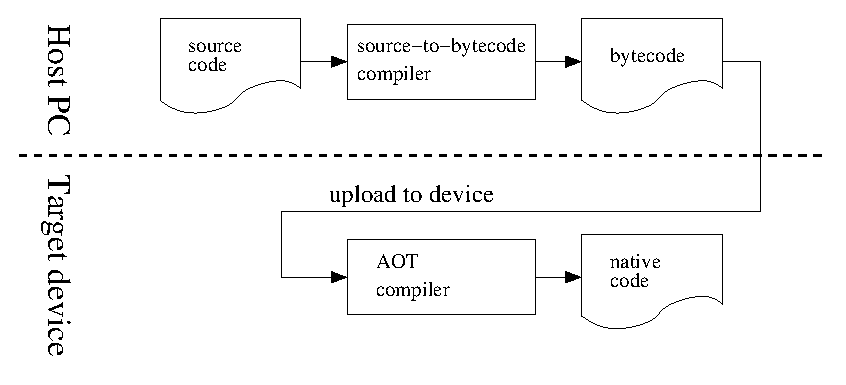
\includegraphics[width=0.8\linewidth]{compilation-process-highlevel.eps}
\caption{High-level overview of the compilation process}
\label{fig-compilation-process-highlevel}
\end{figure}

\paragraph{AOT compiler}
Figure \ref{fig-compilation-process-highlevel} shows the high level process from source code to native code running on the node. The host PC will compile source code to bytecode, which is uploaded to the target node. Instead of interpreting this bytecode, our VM will translate it at load time and store the resulting native code in flash, which is then executed.

We will see that in order to achieve good performance, an optimising source-to-bytecode compiler is necessary to generate high quality bytecode. However, the focus in this dissertation is on the AOT compiler running on the sensor node, and on what performance it can deliver, given good quality bytecode.

Although we will make some changes to the way the bytecode is produced, building a full optimising source-to-bytecode compiler is outside the scope of this dissertation. To determine what level of performance is possible, some manual optimisations are applied to the source code to produce better quality bytecode, most of which an optimising compiler could be expected to do automatically.

\paragraph{Source language}
Note that in Figure \ref{fig-compilation-process-highlevel} we use 'source code' and 'bytecode' instead of Java or JVM bytecode, since the use of Java was only motivated by the availability of existing work to build upon, most notably the Darjeeling VM \cite{Brouwers:2009cj}, not because we believe Java to be a particularly good choice. The techniques described in this dissertation are not specific to Java, but can be applied to any language that compiles to a stack based bytecode.

We will see that in fact Java, in its current form, is not well suited for sensor node applications, and we will end this dissertation with a number of suggestions on how to remedy some of the issues we encountered.


\newpage
\section{Research questions and contributions}
\label{sec-introduction-research-questions}
There are clear advantages to using virtual machines, especially in heterogeneous and dynamic IoT scenarios, but these come at a cost. On a sensor node, this cost is especially significant since they are already very resource-constrained and cannot do many of the optimisations used in VMs on larger devices.

The main research question of this dissertation is whether virtual machines are a suitable means to programme resource-constrained sensor nodes from three perspectives:
\begin{enumerate}
    \item[a.] Performance: How close can an Ahead-of-Time compiling sensor node VM come to native C performance, and what are the trade-offs?
    \item[b.] Safety: Can a VM be an efficient way to provide a safe, sandboxed execution environment on a sensor node?
    \item[c.] Language: Is Java a suitable language for a sensor node VM, and how may it be improved?
\end{enumerate}

\noindent
This dissertation makes the following contributions:
% TODO: read these again
\begin{enumerate}
    \item We identify the major sources of overhead when using the Ahead-of-Time compilation technique described by Ellul and Martinez \cite{Ellul:2010iw, Ellul:2012thesis}.
    \item Using the results of this analysis, we propose a set of eleven optimisations to address each source of overhead. These include improvements to Ellul's AOT approach, modifications to the VM's bytecode, and a lightweight alternative to standard Java method invocation.    
    \item We show that in addition to these improvements to the AOT compiler, better optimisation in the Java to bytecode compiler is critical to achieving good performance.
    \item We describe a number of checks that are sufficient for the VM to provide a safe, sandboxed execution environment, and show most checks can be done at load time, reducing the overhead of run-time checks.
    \item We evaluate our optimisations using a set of benchmarks with varying characteristics, including the commonly used \mybench{CoreMark} benchmark \cite{coremark} and a number of real-world sensor node applications. We show these optimisations:
    \begin{itemize}
    	\item Reduce the size of the generated code by 40\%, allowing larger programmes to be loaded, and quickly compensating for the increase in VM size due to these optimisations,
    	\item Allow constant data to be placed in flash memory, enabling applications with constant tables that otherwise could not be implemented,
    	\item Eliminate 91\% of the performance overhead caused by the VM's stack-based architecture, and 82\% of performance overhead overall.
    \end{itemize}
    \item Using the same benchmarks we evaluate the cost of our safety checks, and show this cost to be comparable to, or lower than the two existing native code approaches to provide a safe execution environment on a sensor node, while providing platform independence at the same time.
    \item Finally, we identify a number of aspects of the Java language and virtual machine that ultimately make it a bad match for sensor nodes, and propose ways to address these issues in future sensor node VMs.
\end{enumerate}

\section{Dissertation outline}
Chapter 2 introduces necessary background knowledge on wireless sensor networks, Java and the Java virtual machine, and AOT compilation.

Chapter 3 discusses the state of the art in improving performance for sensor node VMs and providing a safe execution environment.

Chapter 4 describes the global design of CapeVM.

Chapter 5 first analyses the sources of overhead for the current state of the art in sensor node AOT compilers, and then presents a set of optimisations to address each of these sources. Where there were multiple options to implement an optimisation, we describe alternatives and motivate our choice.

Chapter 6 presents a set of checks that allow CapeVM to provide the sandbox safety guarantees described in Section \ref{sec-introduction-safety}, and shows how the more structured design of the VM's bytecode, compared to native code, allows for most of these checks to be done at load time.

Chapter 7 evaluates the effect of the optimisations presented in Section \ref{sec-optimisations} and the cost of the safety checks presented in Section \ref{sec-safety}.

Chapter 8 describes a number of issues we encountered while doing this work, which show standard Java is not the best choice for a sensor node VM, and suggests ways to improve these in future sensor node VMs.

Chapter 9 concludes this work.

\section{List of publications}
Part of the work presented in this dissertation is based on previously published reports or conference proceedings:

\begin{itemize}
    \item N. Reijers, K. J. Lin, Y. C. Wang, C. S. Shih, and J. Y. Hsu. Design of an Intelligent Middleware for Flexible Sensor Configuration in M2M Systems. \emph{SENSORNETS: Proceedings of the Second International Conference on Sensor Networks}, Feb. 2013.
    \item N. Reijers and C. S. Shih. Ahead-of-Time Compilation of Stack-Based JVM Bytecode on Resource-Constrained Devices. \emph{EWSN: Proceedings of the Fourteenth International Conference on Embedded Wireless Systems and Networks}, Feb. 2017.
    \item N. Reijers and C. S. Shih. Improved Ahead-of-Time Compilation of Stack-Based JVM Bytecode on Resource-Constrained Devices. \emph{arXiv:1712.05590}, Dec. 2017.
    \item N. Reijers, J. Ellul, and C. S. Shih. Making sensor node virtual machines work for real-world applications. \emph{IEEE Embedded Systems Letters}, in press.
\end{itemize}

\section{Naming}
In literature various names are used for our target devices. The word \emph{mote} was common in early research on wireless sensor networks, as was \emph{sensor node}, or simply \emph{device}, although the latter is also used for larger, more powerful devices. In this dissertation we will use the terms \emph{sensor node} or just \emph{node} interchangeably to refer solely to the type of severely resource-constrained devices used in both WSN and IoT applications.

%TODO: do we? actually right now neither term is used very often. Maybe drop this, but should be more consistent.
%The terms \emph{wireless sensor networks}, \emph{cyber-physical systems} and \emph{internet-of-things} are all commonly used to describe sensor node applications. We will use WSN since it is the longer established term, and more clearly focussed on resource-constrained devices, but note that this also covers a large portion of IoT applications.

When reprogramming these nodes, a new programme must be sent to them by a more powerful device. This role is referred to in literature by various names, including \emph{server}, \emph{gateway}, \emph{master}, \emph{controller}, or \emph{host}, depending on the exact design of the network and the way it is reconfigured. For the work in this dissertation these differences are not relevant, and we will use \emph{host} to refer to the source of the code that is uploaded to the sensor node, which is assumed to be a more powerful device with desktop-class processing capabilities.

Since our VM is an Ahead-of-Time compiler, the Java source code is transformed into native code in two steps. We will use \emph{compile time} to refer to the compilation of Java code to bytecode on the host, and \emph{translation time} to refer to the translation of this bytecode into native code on the device.

Finally, we follow Dalvik in naming our virtual machine after a coastal town. In this case the beautiful city of Cape Town, where parts of CapeVM were developed over the course of two trips.

\begin{figure}
\centering
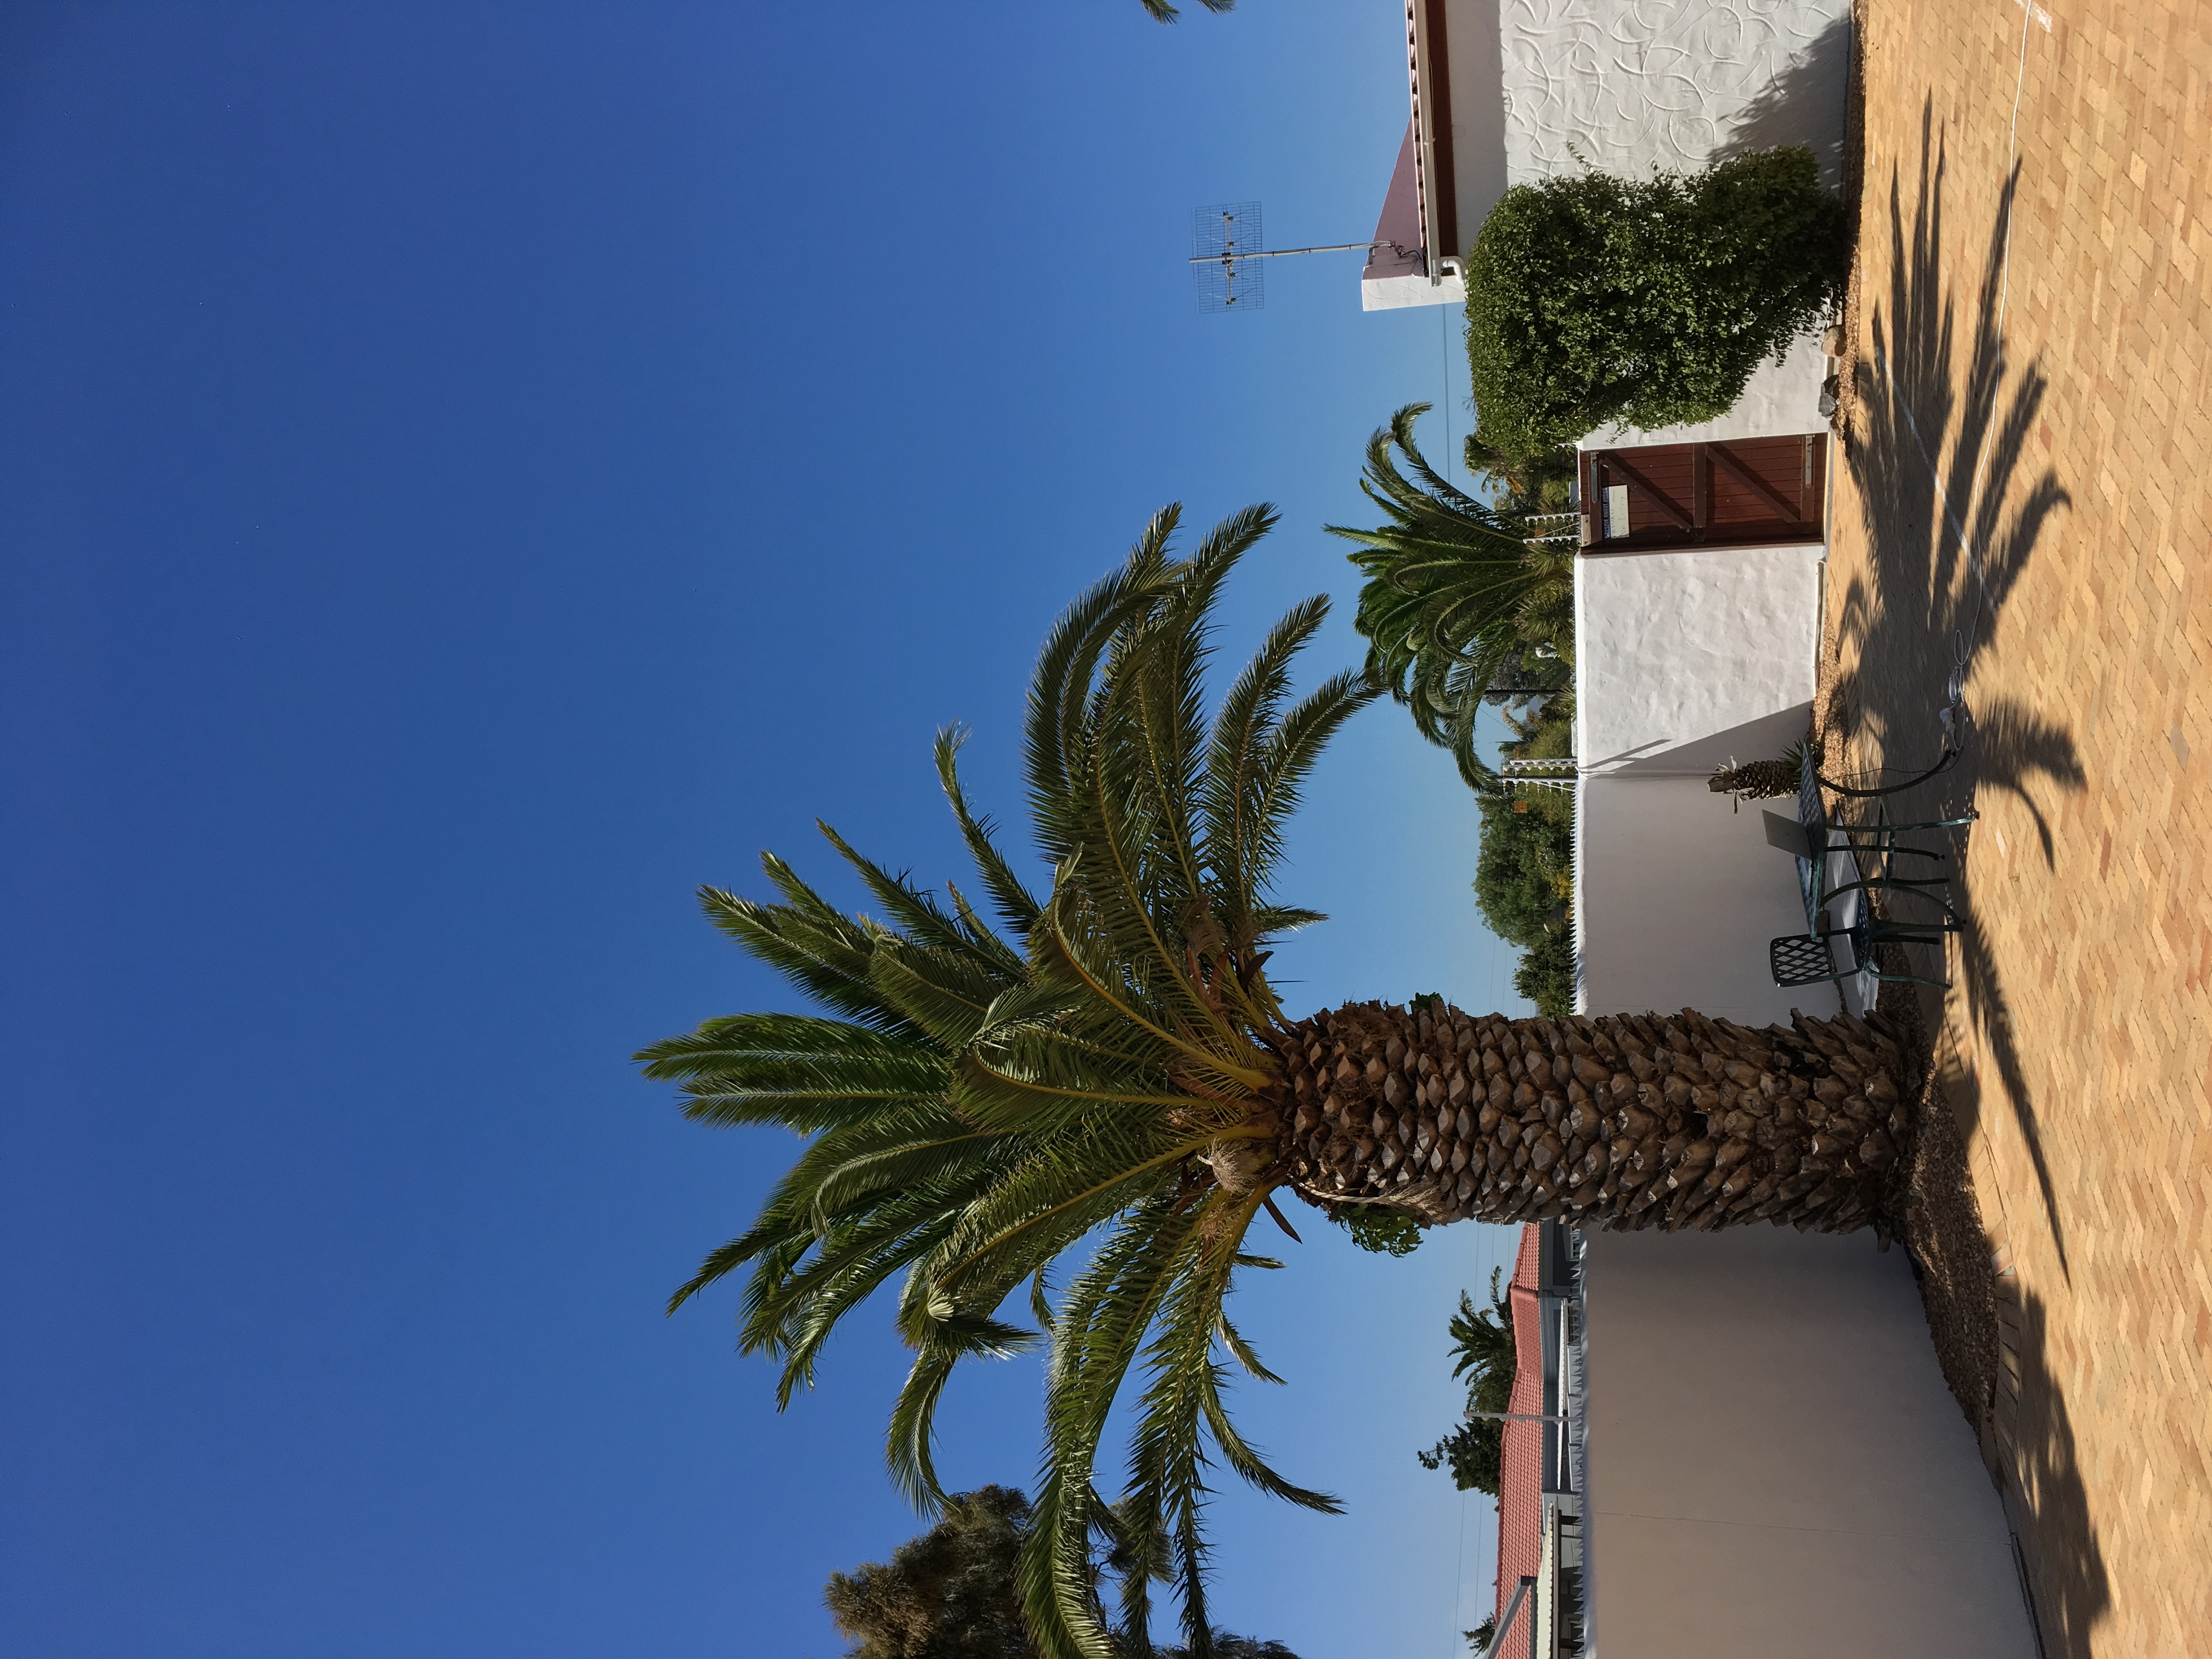
\includegraphics[width=\linewidth,angle=270]{capetown.JPG}
\caption{Cape Town workplace}
\label{fig-capetown}
\end{figure}


\chapter{Background}
to do

% WSN/IoT
% 	classes of devices
% 	typical tiny device
% 		list some characteristics, like REM in the t-kernel paper, but without the E
% Java and JVM bytecode
% 	sandbox
% JIT and AOT compilers


\chapter{State of the art}
This chapter presents the state of the art in Internet of Things and sensor networks relevant to the work in this dissertation. It starts with existing work on programming WSN and IoT networks, and the virtual machines developed for them. Next, it discusses proposed ways to improve sensor node VM performance, and ways to guarantee safety on sensor devices.

\section{Programming WSN and IoT devices}

This challenge of programming IoT devices can be split into two questions:

\begin{itemize}
    \item How can we build applications at a higher level, coordinating the behaviour of many devices without having to specify the behaviour from each device's individual perspective?
    \item How can we best reprogramme individual nodes safely and efficiently to support these applications?
\end{itemize}

This dissertation is concerned with the second question, and argues that a virtual machine can be an attractive option in many scenarios. But we will first discuss the higher level question of how to programme WSN/IoT applications and use one of these systems as a motivating example.

Initially, many WSN applications were built directly on top of the hardware or on some minimal operating system, such as TinyOS \cite{Levis:2004ws}. This results in applications being programmed from the individual node's perspective, rather than allowing the developer to express globally what he wants from the sensor network, which makes it hard to reason about the global behaviour, especially as the number of devices and tasks increases.

Therefore, systems have been developed that make it easier for the developer to control the potentially larger number of heterogeneous nodes. Some of these are centralised, where the initiative of the application is with some central host, and devices are loaded with a runtime that allows the host to control them. Other systems are more distributed, where the application is split into components that are deployed onto nodes and from there operate more autonomously, only to receive further guidance from the host where necessary.

In the first category fall systems like sMap \cite{DawsonHaggerty:2010eo}, which provides an attractive and flexible RESTful interface to a sensor network through which we can discover what sensors are available at a certain node and get or set several configuration properties. Although the authors succeeded in dramatically reducing the footprint, it is still relatively resource intensive. It is also limited in the number of properties it exposes, but the idea could easily be expanded. Similarly TinyDB \cite{Madden:2005tj} also makes an entire network of sensor nodes available through a central interface, in this case a SQL-like query language.

ADAE \cite{Chang:2010ek}, developed at the IT University of Copenhagen, configures the network according to a policy describing the desired data quality, including fallback options which the system may use in case the ideal situation cannot be achieved. ADAE then dynamically reconfigures the network in response to changing conditions such as node failures, unexpected power drops, or interesting events detected by the network. However, the language used to describe the policy and constraints is hard to use and it is likely a skilled engineer is needed to translate the user's requirements into the constraint optimisation problem ADAE uses as input.

While in the previous systems applications run on a centralised host and simply control the nodes in the network, in Agilla \cite{Fok:2005bh} programmes are more distributed and consists of software agents that can move around in the network autonomously. While this allows some behaviours to be expressed in a natural way, the paradigm is very different from conventional languages, and the assembly-like instruction set based on the Maté VM \cite{Levis:2002ku} discussed below makes it hard to use.

Cornell's MagnetOS \cite{Liu:2005wsa}, proposes a novel programming model which allows the user to write the application as a single Java application, not explicitly related to individual nodes. The system then automatically partitions the applications into pieces (by default along object boundaries), and places these pieces on nodes in the network in such a way as to minimise energy consumption. However, it requires nodes significantly more powerful than what we expect to find in a typical WSN.

LooCI \cite{Hughes:dg} is a component infrastructure middleware for WSNs with standard support for run-time reconfiguration. The LooCI component model supports dynamic binding and interoperability between different hardware platforms, in their case a typical sensor node and the slightly more powerful Sun SPOT, and different languages, with implementations in C and Java. LooCI defines a list of requirements for WSN middleware, which includes supporting run-time reconfiguration to respond to changing environmental conditions, supporting heterogeneous sets of hardware, good performance, and minimal memory consumption. LooCI currently uses C to programme the smallest devices and Java for the more powerful Sun SPOT. A fast sensor node virtual machine would be a useful addition to allow more flexible and platform independent reprogramming of the smallest devices as well.

\section{WuKong}
\label{sec-state-of-the-art-wukong}
A final example that we will look at in more detail at is WuKong \cite{Reijers:2013ut, Lin:2013dc}.


\begin{figure}
\centering
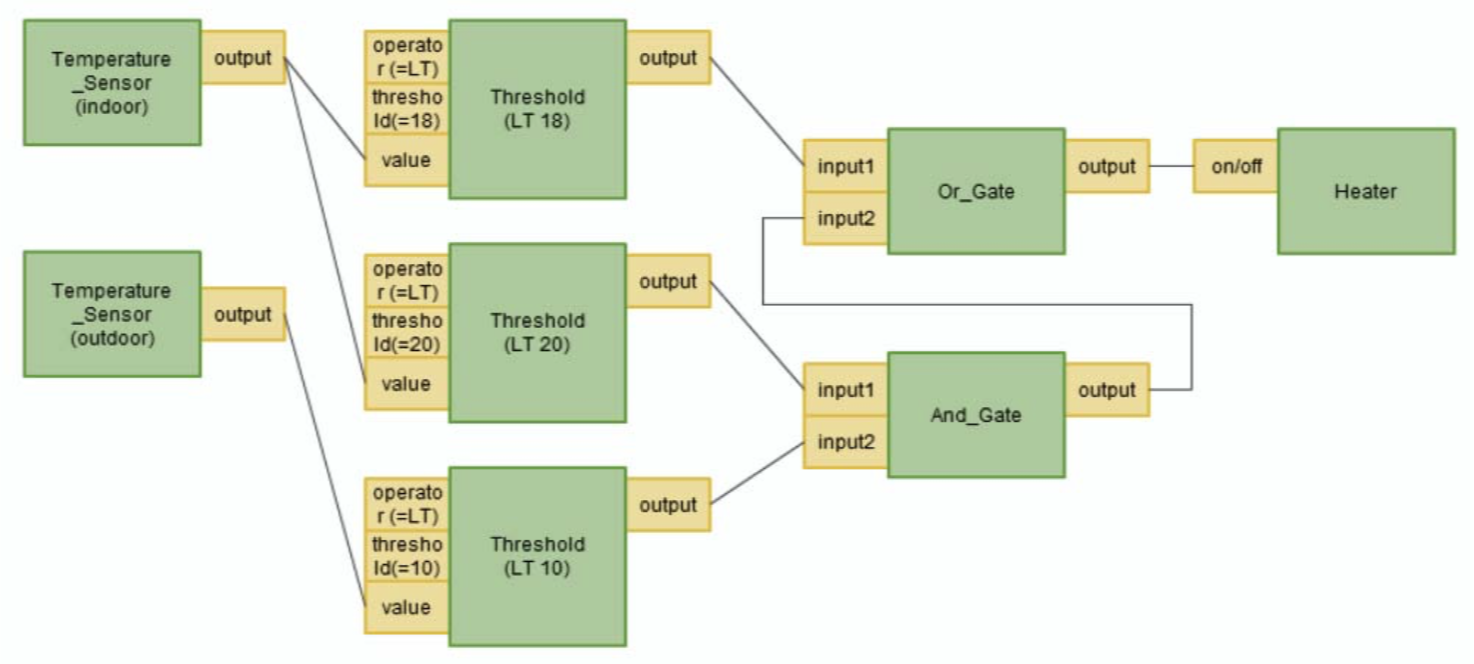
\includegraphics[width=0.8\linewidth]{wukong-fbp.png}
\caption{Example WuKong flow based programme}
\label{fig-wukong-fbp}
\end{figure}


Applications in WuKong are written in the form of a flow based programme, an example of which is shown in Figure \ref{fig-wukong-fbp}. Components are called WuObjects, and are instances of WuClasses. Each WuClass defines a number of input and output properties. For example, the Temperature Sensor WuClass has a single 'output' property, while the Heater has a single 'on/off' property.

When deploying an application, the host, called \emph{master} in WuKong, will first discover the available resources in the network and then try to find a node to deploy each component to.

A node creates WuObjects to represent its hardware components at startup, so the master can discover the sensors and actuators available in the network. When deploying the application, the master may use a hardware WuObject by connecting its properties. For software components, like the Threshold or And\_Gate in the example, the master may create new instances on a node.

An WuClass is defined by:
\begin{itemize}
    \item Its list of properties.
    \item A \mycode{setup()} function, called once when an object is created.
    \item A \mycode{update()} function, called (i) periodically, for example to sample a sensor, or (ii) when one of the input properties changes value, to compute a new output value or drive an actuator.
\end{itemize}

The \mycode{setup()} and \mycode{update()} functions can be written in either C or Java. A node may have native C implementations built in for a number of commonly used classes from the WuKong standard library, which it will advertise during the discovery phase. If the master cannot find a native implementation of a required class, it may use a Java version instead, which is slower, but more flexible since it can be deployed as part of the application. To support this, the WuKong middleware contains a version of the Darjeeling JVM \cite{Brouwers:2009cj}.


The WuKong middleware takes care of propagating property changes along the links drawn in the FBP. For example, if in Figure \ref{fig-wukong-fbp} the output of the Or\_Gate changes, the new output value is automatically propagated to the Heater's on/off property, and the Heater's \mycode{update()} function is called. An application in WuKong is defined by a number of compact tables, describing the components and links between them, and optionally a number of Java WuClasses.

In WuKong's vision, the master dynamically manages the network. A node may be used in multiple applications, and its tasks may change while the application is running if the master decides to reconfigure the network, for example in response to failure \cite{Su:2014uf} or because network conditions change.


\section{Sensor node virtual machines}
Many VMs have been proposed that are small enough to fit on a resource-constrained sensor node. They can be divided into two categories: generic VMs and application-specific VMs, or ASVMs \cite{Culler05} that provide specialised instructions for a specific problem domain.

As an example, designed specifically for wireless sensor networks, Mat\'e \cite{Levis:2002ku} was one of the first to prove sensor nodes can run a virtual machine. It provides single instructions for tasks that are common on a sensor node, so programmes can be very short.  

SwissQM \cite{Muller:2007fs} is a more traditional and more powerful VM, based on a subset of the Java VM, but extended with sensor network specific instructions to access sensors and do data aggregation. In both systems however, the application has to be programmed in very low level, assembly-like language, limiting their target audience.

VM* \cite{Koshy:2005ww} sits halfway between the generic and ASVM approach. It is a Java VM that can be extended with new features according to application requirements. Unfortunately, it is closed source.

Several generic VMs for high level languages like Python, LISP, and Java have also been developed, which fit on severely resource-constrained nodes. Almost all rewrite the original bytecode to their own format and employ various techniques to reduce code size. Some functionality is sacrificed in order to fit on the sensor nodes, for instance reflection or floating point datatypes are typically not supported.

The Python-on-a-chip project \cite{python-on-a-chip} developed a Python bytecode interpreter small enough to fit on sensor nodes. Requiring 55 KB of flash memory and a recommended 8 KB of RAM, it fits on many, but not all of the current sensor boards. MicroPython \cite{micropython} requires slightly more hardware at 256 KB flash memory and 16 KB RAM, but has its own hardware platform and runs Python 3.

LISP is one of the first high-level languages, developed at a time when room-sized computers had only slightly more capabilities than current sensor nodes. SensorScheme \cite{Evers:2010ur} implements a fully functioning LISP interpreter in under 41 KB, and is one of the few sensor node VMs to provide a safe execution environment.

CILIX \cite{Kishino:2010} is a small VM for the .Net Common Intermediate Language implemented on the MSP430. MoteRunner \cite{Caracas:2009} runs on similar devices. Instead of implementing an existing VM it targets all strictly typed programming languages and supports both Java and C\#.

The smallest official Java standard is the Connected Device Limited Configuration \cite{CLDC}, but since it targets devices with at least a 16 or 32-bit CPU and 160-512 KB of flash memory available, it is still too large for most sensor nodes. As a result, a number of Java VMs have been developed for sensor nodes, all offering some subset of the standard Java functionality, occupying different points in the trade-off between the features they provide, and the resources they require.

Darjeeling \cite{Brouwers:2009cj} from Delft University of Technology runs a modified Java bytecode with only minor restrictions, and supports multiple platforms. Similarly, TakaTuka \cite{Aslam:2008} also runs on both AVR and MSP based sensor nodes, and includes its own debugger. A unique property is TakaTuka's ability to reduce garbage collection cost by static code analysis. Whenever the compiler can determine an object can be safely discarded at a certain point, it annotates the bytecode to tell the VM to do so, thus freeing up memory earlier and reducing the number of times the garbage collector has to run. 

Sun's Squawk VM \cite{Shaylor:2003ws} is significantly larger than Darjeeling and TakaTuka, requiring at least 160 KB of programme memory, but offers full CLDC compliance. The Java Card VM \cite{javacard} runs on more typical sensor node hardware and achieves this by also switching to a 16-bit architecture, dropping support for various features, and modifying the instructionset. At the smallest end of the spectrum is NanoVM \cite{Harbaum}, which takes a minimal approach, trading support for a large number of java opcodes for simplicity and code size. The whole VM fits in the 8K flash of an ATmega8 CPU, leaving 512bytes of EEPROM and 75\% of the CPU's 1K RAM to the application.

\section{Darjeeling}
Since our VM is based on Darjeeling, we will examine it in more detail in this section.

\paragraph{Split VM architecture}
\begin{figure}
\centering
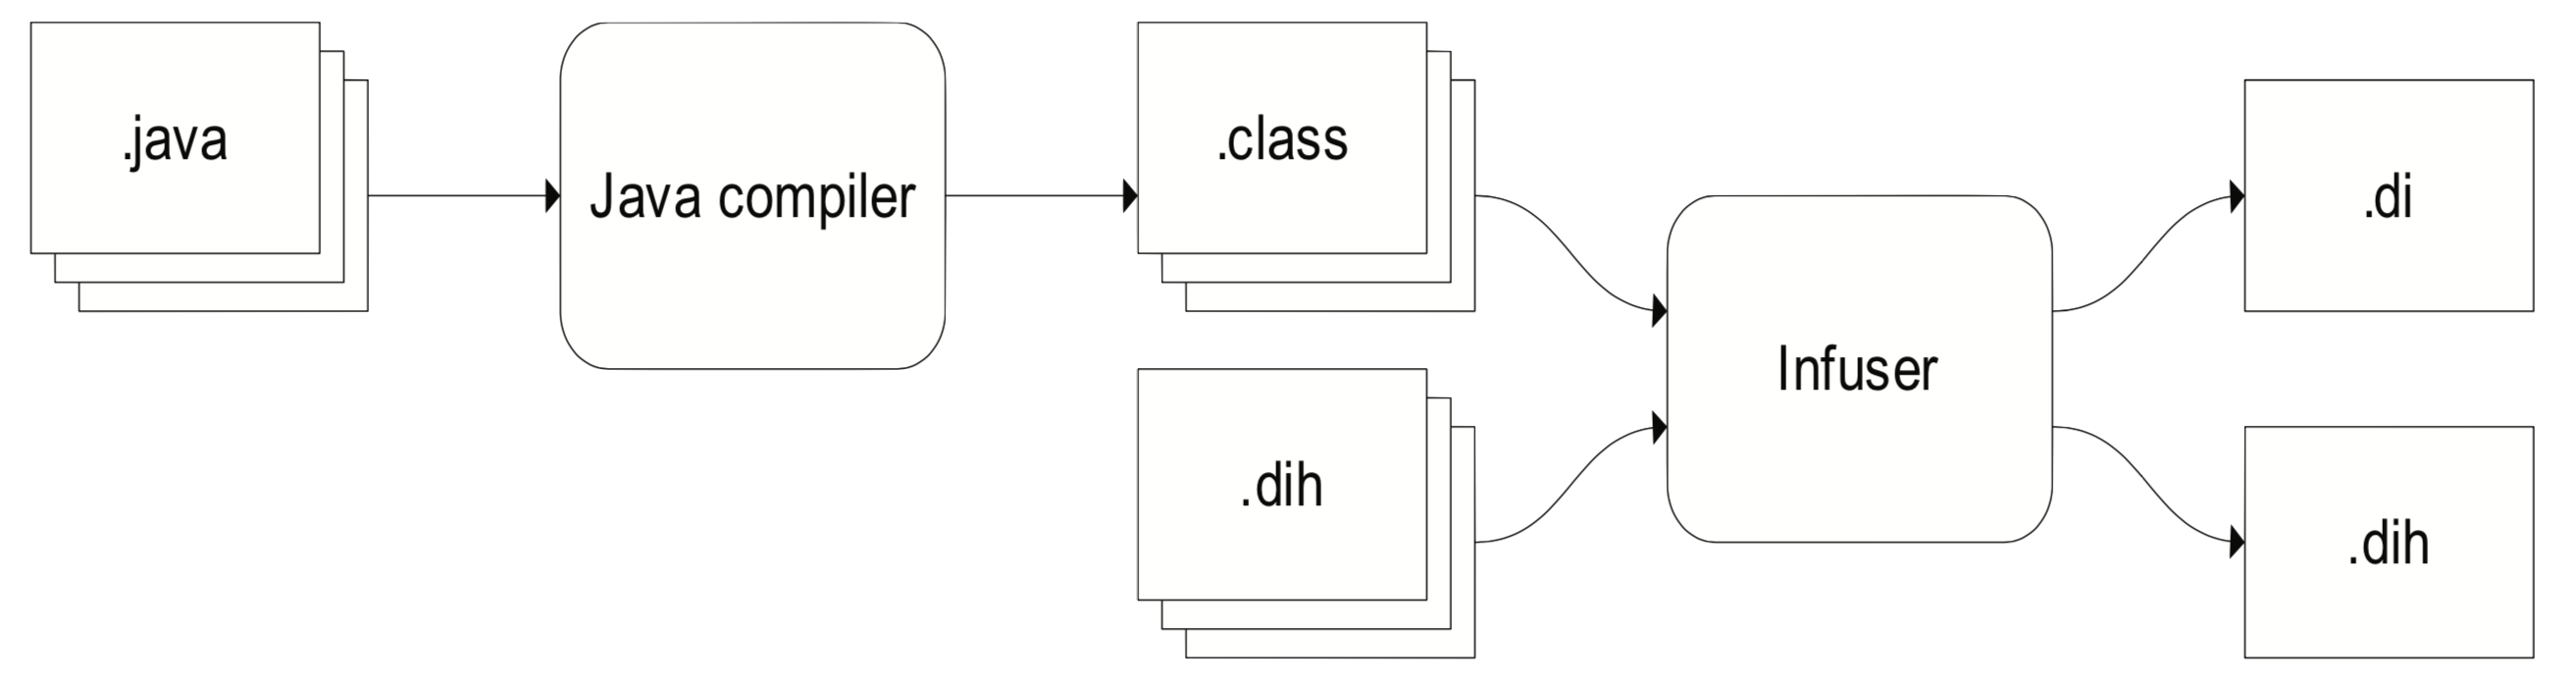
\includegraphics[width=0.6\linewidth]{darjeeling-infusion-process}
\caption[Darjeeling infusion process]{Darjeeling infusion process, source: \cite{Brouwers:2009cj}}
\label{fig-darjeeling-infusion-process}
\end{figure}
Like most other sensor node JVMs, it uses a \emph{split VM architecture} \cite{Simon:2006wd}. The virtual machine running on the node does not use standard JVM class files, but these class files are first transformed by an offline tool into a format more suitable for a sensor node. In Darjeeling's case this tool is called the \emph{infuser}, which takes several Java classes and statically links them into a single \emph{infusion}.

The infuser changes the bytecode in several ways, replacing named references by a numbering scheme, so that the constant strings with class and method names can be removed from the constant pool, and statically linking the Java classes into a flattened list entities. Infusions are typically libraries, such as the \mycode{java.lang} base library, networking protocols, or the application. An infusion can reference code in another infusion using header files, created during the infusion process that allow the infuser to find the numbered identifiers of classes and methods in referenced infusions. This is shown in Figure \ref{fig-darjeeling-infusion-process}.

\paragraph{16-bit architecture}
\begin{figure}
\centering
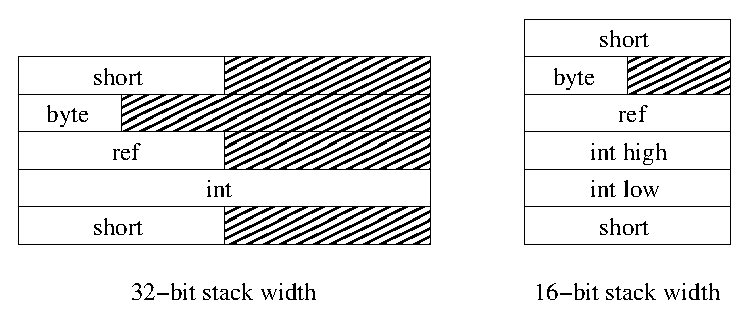
\includegraphics[width=0.6\linewidth]{32bit-vs-16bit-stack}
\caption{Unused memory for 32 and 16-bit slot width}
\label{fig-32bit-vs-16bit-stack}
\end{figure}

Besides statically linking classes, the infuser also makes several changes to the bytecode format. References on sensor nodes are usually 16-bit, and 8-bit and 16-bit integer variables are commonly used in sensor node code to save memory. Storing all data in 32-bit slots as the JVM does would lead to significant overhead, as shown in Figure \ref{fig-32bit-vs-16bit-stack}. Therefore, Darjeeling's stack and variable slots are 16-bit wide, using two slots for 32-bit ints, similar to how the normal JVM uses two 32-bit slots for 64-bit longs. Darjeeling's bytecode also introduces 16-bit versions of many opcodes, for example \mycode{SADD} adds two 16-bit shorts, while \mycode{IADD} adds two 32-bit ints. The infuser analyses the type of expressions, and replaces the 32-bit instructions found in normal JVM bytecode with the 16-bit variants where possible.



\paragraph{Double-ended stack}
\begin{figure}
\centering
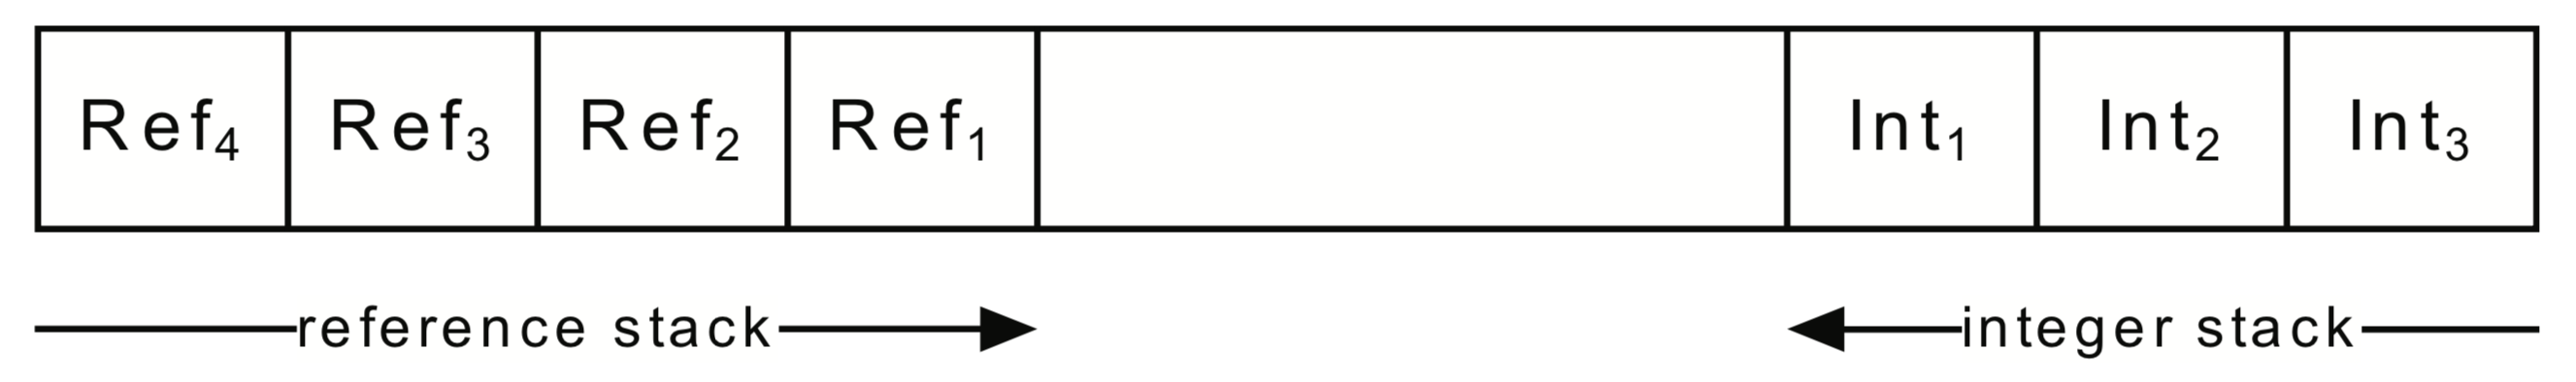
\includegraphics[width=0.6\linewidth]{darjeeling-split-stack}
\caption[Darjeeling split operand stack]{Darjeeling split operand stack, source: \cite{Brouwers:2009cj}}
\label{fig-darjeeling-split-stack}
\end{figure}

A second important modification is that Darjeeling splits the operand stack into separate reference and integer stacks, as shown in Figure \ref{fig-darjeeling-split-stack}. Each stack frame still allocates the same amount of space for its operand stack, but Darjeeling places references on one side, and integers on the other. At the expense of having to keep track of two operand stack pointers, this reduces the complexity of the garbage collector significantly. When the garbage collector runs, it needs to find the \emph{root set} of all live objects, which includes objects with references on the stack but not stored elsewhere. Since the type of the values on the operand stack changes continuously, it would be hard to determine which values are references and which are integers in a single stack, but using Darjeeling's split stack design, it can simply place all values on the reference stack in the root set. For the same reason, Darjeeling also groups the slots allocated for local, static and instance variables into an integer and reference group.

The necessary modifications to the bytecode are taken care of by the infuser. Generic stack instructions such as \mycode{pop} are replaced by distinct versions for the integer and reference stack: \mycode{ipop} and \mycode{apop}.

\paragraph{Limitations}
Darjeeling implements a significant subset of Java, but like all sensor node JVMs it needs to make some sacrifices to scale down to sensor node size. Specifically, it does not support the 64-bit \mycode{long} datatype or floating point variables. It does not support reflection, since the infusion process drops the necessary type information from its class files to significantly reduce their size. Darjeeling also does not support the \mycode{synchronized} modifier on static methods, but it can be easily simulated using synchronized blocks, which are supported.

\section{Performance}
While many different VMs have been published, only a few papers describing sensor node VMs contain detailed performance measurements, shown earlier in Table \ref{tbl-slowdown-for-sensornode-vms}. Darjeeling \cite{Brouwers:2009cj} reports between 30x and 113x slowdown for 3 benchmarks in 16-bit and 32-bit variations, compared to the native C equivalent. Ellul \cite{Ellul:2012thesis} reports measurements on the TakaTuka VM \cite{Aslam:2008} where the VM is 230x slower than native code, and consumes 150x as much energy. TinyVM \cite{Hong:2012wj} is between 14x and 72x slower than C, for a set of 9 benchmarks. DVM \cite{Balani:2006} has different versions of the same benchmark, where the fully interpreted version is 108x slower than the fully native version, while Kumar reports a slowdown of 555x for the same VM \cite{Kumar:2007ge}. Finally, SensorScheme \cite{Evers:2010ur} is up to 105x slower. Since performance depends on many factors, it is hard to compare these numbers directly. But the general picture is clear: current interpreters are one to two orders of magnitude slower than native code.

Translating bytecode to native code to improve performance has been a common practice for many years. A wide body of work exists exploring various approaches, either offline, ahead-of-time  or just-in-time. One common offline method is to first translate the Java code to C as an intermediate language, and take advantage of the high quality C compilers available \cite{Dean:1996wb, Muller:1997}. Courbot et al. describe a different approach, where code size is reduced by partly running the application before it is loaded onto the node, allowing them to eliminate code that is only needed during initialisation \cite{Courbot:2010}. Although the initialised objects are translated to C structures that are compiled and linked into a single image, the bytecode is still interpreted. While in general we can produce higher quality code when compiling offline, doing so sacrifices the key advantages of using a VM.

Hsieh et al. describe an early ahead-of-time compiling desktop Java VM \cite{Hsieh:1996cy}, focussing on translating the JVM's stack-based architecture to a register based one. In the Japale\~no VM, Alpern et al. take an approach that holds somewhere between AOT and JIT compilation \cite{Alpern:1999}. The VM compiles all code to native code before execution, but can choose from two different compilers to do so. A fast baseline compiler simply mimics the Java stack, but either before or during run time, a slower optimising compiler may be used to speed up critical methods.

Since JIT compilers work at run time, much effort has gone into making the compilation process as light weight as possible. For example Krall \cite{Krall:1998} reduced the compilation time in early JIT compilers using a more lightweight register allocation algorithm. While the goals are similar to ours, this approach requires three passes over the code and significantly more complex data structures than a sensor node could handle. More recently these efforts have included JIT compilers targeted specifically at embedded devices. Swift \cite{Zhang:2012wf} is a light-weight JVM that improves performance by translating a register-based bytecode to native code. But while the Android devices targeted by Swift may be considered embedded devices, they are still quite powerful and the transformations Swift does are too complex for the ATmega class of devices. HotPathVM \cite{Gal:2006} has lower requirements, but at 150 KB for both code and data, this is still an order of magnitude above our target devices.

Given our extreme size constraints - ideally we only want to use in the order of 100 bytes of RAM to allow our approach to be useful on a broad range of devices, and leave ample space for concurrent tasks running on the device - almost all AOT and JIT techniques found in literature require too much resources. Indeed, some authors suggest sensor nodes are too restricted to make AOT or JIT compilation feasible \cite{Aslam:2011thesis, Wirjawan:2008}.

\section{AOT compilation for sensor nodes}
\label{sec-state-of-the-art-elluls-aot}
On the desktop, VM performance has been studied extensively, but for sensor node VMs this aspect has been mostly ignored. To the best of our knowledge AOT compilation on a sensor node has only been done by Ellul and Martinez \cite{Ellul:2010iw, Ellul:2012thesis}, and this work builds on theirs.

Their approach is both simple and effective. To translate the JVM bytecode, each bytecode instruction is replaced by a fixed sequence of native instructions that implements it. This can be done in a single pass, as the bytecode is being received by the node, writing blocks of native code to flash memory instead of JVM bytecode. Like Darjeeling, they use a split stack architecture, with the CPU's native stack doubling as integer operand stack, while reference operands are still stored in the stack frame.

\begin{table}
\caption[Example of Ellul's AOT translation of \mycode{c=a+b;}]{Example of Ellul's AOT translation of \mycode{c=a+b;}, source: \cite{Ellul:2012thesis}}
\label{tbl-ellul-aot-example}
    \begin{tabular}{llll} % NO SIMULATION DATA
    \toprule
    Bytecode  & Stack before        & Stack after         & Native pseudo assembly code \\
    \midrule
    \midrule
    ILOAD\_0  & ...                 & ...                 & LOAD r1, a \\
              & ...                 & ..., value1         & PUSH r1 \\
    ILOAD\_1  & ..., value1         & ..., value1         & LOAD r1, b \\
              & ..., value1         & ..., value1, value2 & PUSH r1 \\
    IADD      & ..., value1, value2 & ..., value1         & POP r1 \\
              & ..., value1         & ...                 & POP r2 \\
              & ...                 & ...                 & ADD r1, r2 \\
              & ...                 & ..., result         & PUSH r1 \\
    ISTORE\_2 & ..., result         & ...                 & POP r1 \\
              & ...                 & ...                 & STORE c, r1 \\
    \bottomrule
    \end{tabular}
\end{table}

Table \ref{tbl-ellul-aot-example} shows how a simple statement is translated to native code. The blocks each JVM bytecode instruction translates to are fixed. This simple translation to native code removes the interpreter loop, which is by far the biggest source of overhead in interpreting VMs, but it is clear from the native pseudo code in Table \ref{tbl-ellul-aot-example} that this approach results in many unnecessary push and pop instructions. Since the JVM is a stack-based VM, each instruction first obtains its operands by popping them from the stack and pushes any result back onto it. As a result, over half the instructions are push or pop instructions.

\subsection{Peephole optimisation}
To reduce this overhead, Ellul proposes a simple peephole optimiser \cite{Ellul:2012thesis} which does 4 optimisation. For each an example is shown in Table \ref{tbl-ellul-peephole}. The first to are the most important for improving performance: if a push is immediately followed by a pop to the same register, both are removed since they have no net effect. If the source and destination registers differ, the two instructions are replaced by a move. Note that the assembly code shown here is for the MSP430 CPU used in Ellul's work.

\begin{table}
\caption{Ellul's peephole optimisations}
\label{tbl-ellul-peephole}
    \begin{threeparttable}
    \begin{tabular}{lrrlrr} % NO SIMULATION DATA
    \toprule
    Before            &        &        & After             &        & \\
    Instructions      & Cycles & Length & Instructions      & Cycles & Length \\
    \midrule
    \midrule
    PUSH R13          & 6      & 2      &                   & 0      & 0 \\
    POP R13           &        &        &                   &        & \\
    \midrule
    PUSH R13          & 6      & 2      & MOV R13, R14      & 1      & 1 \\
    POP R14           &        &        &                   &        & \\
    \midrule
    MOV \#0, R15      & 2      & 2      & CLR R15           & 2      & 1 \\
    \midrule
    MOV R6,R5         & 5      & 3      & MOV R6,0x0000(R4) & 4      & 2 \\
    MOV R5,0x0000(R4) &        &        &                   &        & \\
    \bottomrule
    \end{tabular}
    \begin{tablenotes}
    \item MSP430 assembly, source: \cite{Ellul:2012thesis}
    \end{tablenotes}
    \end{threeparttable}
\end{table}

\subsection{Resulting performance}
Ellul's approach improves performance considerably compared to interpreters, but using the standard \mybench{CoreMark} benchmark \cite{coremark}, it generates code that is still up to 9.1x slower than optimised native C.

It is important to further improve this for a number of reasons. First, even if an application is asleep for a large percentage of the time, it may at times want to measure something at high resolution, similar to how ADAE \cite{Chang:2010ek} responds to what it calls 'interesting events' by taking extra measurements as long as its energy budget permits. Any slowdown in the VM will affect the maximum rate at which such samples can be taken. Similarly, Table \ref{tbl-amulet-applications-sleep} shows that for the Amulet smart watch platform, a 9.1x slowdown in the application code means the CPU is not fast enough to finish the some of the application's tasks in time. At best this would result in slower response time or sampling rates, at worst in could result in incorrect behaviour.

Second, reduced performance means the CPU has to stay active for a longer time, resulting in increased cpu power consumption and reduced battery life. Looking at the calculations for lossless compression in Section \ref{sec-introduction-performance}, the ratio of the energy saved on radio transmission vs energy spent on compression was about 2.6:1. This result depends on many factors, for instance less than ideal network conditions may cause retransmissions, increasing the cost per bit sent and making compression more worthwhile. However in this particular case the slowdown incurred even after Ellul's optimisation would make compression a net loss. Any slowdown will push some situations past the break-even point, or reduces the benefits of compression in others.

There are scenarios that may not be able to tolerate the one to two orders of magnitude slowdown seen in interpreters, but where a slowdown of up to 9.1x for Ellul's AOT approach may be acceptable. However, there is a third reason to improve on it: it results in code which is on average 3.3 times larger than the native equivalent. This reduces the amount of code we can load onto a node, and given that flash memory is already restricted, this is a major sacrifice to make when adopting AOT compilation on sensor nodes.


\section{Safety}
\label{sec-state-of-the-art-safety}
With some exceptions \cite{Evers:2010ur}, most current sensor node VMs do not discuss safety, but instead focus on the functionality provided and how this can be implemented on a tiny sensor node. This is unfortunate, because the ability to provide a safety execution environment is both desirable, and easier to implement using a VM than it is using native code.

\begin{figure}
\centering
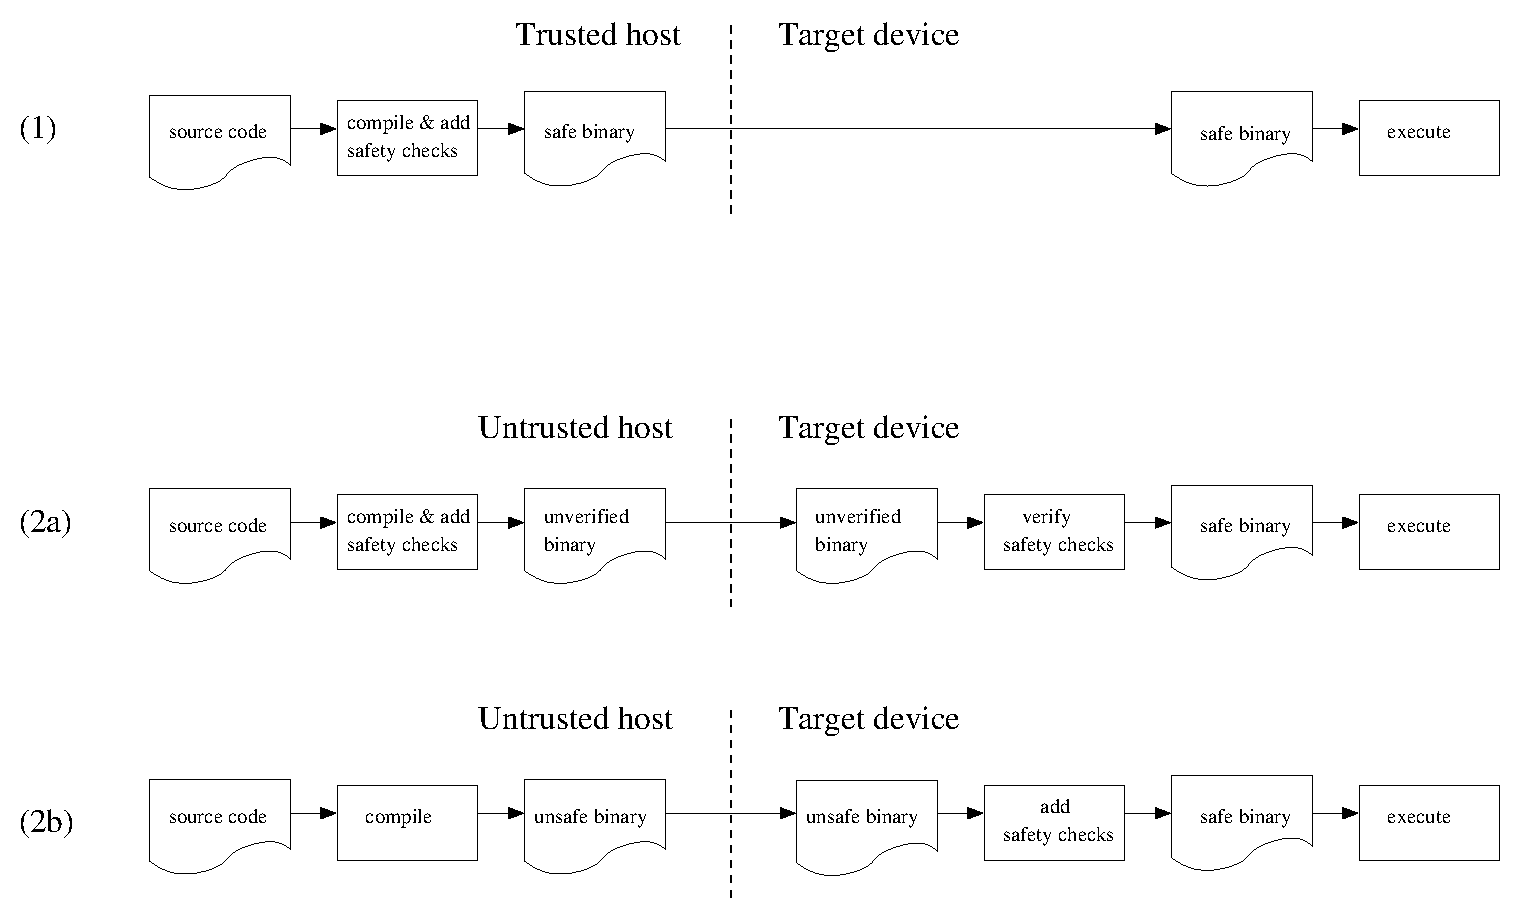
\includegraphics[width=\linewidth]{safe-compilation-process.eps}
\caption{Three approaches to provide a safe execution environment}
\label{fig-safe-compilation-process}
\end{figure}

Several non-VM systems exists to provide safety for sensor nodes. They fall into two distinct categories, as shown in Figure \ref{fig-safe-compilation-process}. If we trust the host, it can verify the code and add run-time safety checks where needed, before the code is sent to the node. However, to allow the node to receive code from untrusted sources, for example to support mobile agents as in Agilla \cite{Fok:2005bh}, it needs to guarantee safety independent of a host to guard against bugs and malicious attacks. The latter is obviously the stronger guarantee, but it also comes at a higher price.

\subsection{Source code approaches}
\label{sec-state-of-the-art-source-code-safety}
In the first category are systems that guarantee safety at the source code level. Virgil \cite{Titzer:2006uy} is a language that is inherently safe and specifically designed for sensor nodes. The application is explicitly split into an initialisation and run-time phase, where objects are only allocated during the initialisation phase. The initialisation phase happens during compilation (to C code), which means all object and their locations are know at this point, allowing Virgil to ensure safety and optimise the code at compile time.

Safe TinyOS \cite{Cooprider:2007ub} on the other hand, works on annotated nesC TinyOS code. It uses the Deputy \cite{Condit:2007uo} source-to-source compiler to analyse the C source code and insert the necessary run-time checks were necessary. Because this happens on the host, before sending the code to the node, it can use the host's resources to do more complex analysis of the source code and eliminate checks where the it can determine a memory access to be safe at compile time, resulting in a much lower overhead

Similarly, applications for the Amulet \cite{Hester:2016je} smart watch platform are written in a restricted version of C that removes many of C's riskier features. Run-time checks are then added for operations where static analysis cannot guarantee them to be safe. Ongoing research in the Amulet project is on using hardware memory protection units found in some CPUs to reduce the cost of these restrictions and safety checks \cite{Hardin:2017cq}, but at the time of writing no results had been published.

All three approaches eventually result in standard C, which is then compiled and sent to the node. Therefore, these approaches may protect against accidental programming errors, but not against malicious code sent to a node.

\subsection{Native code approaches}
For desktop applications, Wahbe et al. described software fault isolation \cite{Wahbe:1994cj} techniques to isolate a piece of untrusted code, without the overhead of using processes and the CPU's memory protection. A typical example is a plugin that frequently needs to interact with an application. It should be isolated from the application so bugs in the plugin cannot bring down the whole application, but running it as a separate process would incur a high overhead.

Two basic methods are described to isolate such code from the main application: the native code can be rewritten at load time, inserting checks at all potentially unsafe writes, or it can be compiled to a predefined format with the appropriate checks already in place, after which the system loading the code only verifies it adheres to this standard at load time.

Since we do not have processes or CPU memory protection on a sensor node, Wahbe's approach provides an attractive alternative. Two systems exist that provide safety for sensor nodes using each of these approaches.

\emph{t-kernel} \cite{Gu:2006ww} does more than providing memory safety. It raises the level of system abstraction for the developer by providing three features typically missing on sensor nodes: preemptive scheduling, virtual memory, and memory protection. It does this by extensive rewriting of the binary code at load time. While \emph{t-kernel} is heavily optimised, the price for this is that programmes still run 50-200\% slower, and code size increases by 500-750\%.

The other approach is taken by Harbor \cite{Kumar:2007ge}, which consists of two components. On the desktop, a binary rewriter sandboxes an application by inserting run-time checks before it is sent to the node. The SOS operating system \cite{Han:2005th} is extended with a binary verifier to verify incoming binaries have the necessary checks in place. The correctness only depends on the correctness of this verifier. The increase in code size is more modest than for \emph{t-kernel} at a 30-65\% increase, but performance is 160-1230\% slower. They also note more complex analysis of the binary code could reduce the number of necessary checks, but at the cost of significantly increasing the complexity of the verifier.

Finally, Weerasinghe and Coulson \cite{Weerasinghe:2008kh} proposed a system for module isolation similar to Harbor in the sense that code is compiled to a restricted, safe form of native code which is then verified by the node. Memory is allocated in fixed sized, aligned blocks, where a block size of 256 is suggested to simplify the verifier since the split between block address and offset falls nicely along byte boundaries. The authors aim to minimise run-time overhead and identify \emph{t-kernel} code size overhead as a major drawback of this approach. Unfortunately their implementation was not yet finished when their paper was published and no further publications on this approach could be found.

\chapter{CapeVM}

This chapter we introduce the global design of CapeVM, which is a modified version of Darjeeling \cite{Brouwers:2009cj}. It runs directly on the hardware, without any OS layer in between, and has complete control over the device. CapeVM modifies Darjeeling in three ways:
\begin{itemize}
    \item AOT compilation: Darjeeling is originally an interpreter. To improve performance, this interpreter is replaced with an Ahead-of-Time compiler: instead of interpreting the bytecode, CapeVM translates it to native code at load time, before the application is started. While JIT compilation is possible on some devices \cite{Ellul:2012thesis}, it depends on the ability to execute code from RAM, which many embedded CPUs, including the ATmega, cannot do.
    \item Bytecode format: To support the AOT compilation process and further improve performance, CapeVM modifies Darjeeling's bytecode format, and adds several new bytecode instructions.
    \item Safety: CapeVM adds a number of translation-time and run-time safety checks to provide a safe, sandboxed execution environment.
\end{itemize}

\section{Goals}
\label{sec-CapeVM-goals}
Working on resource-constrained devices means we have to make some compromises. Our main goal is to build an AOT compiling VM that generates safe code, performs well, reduces the code size overhead seen in previous work, and fits as many IoT scenarios as possible. This includes scenarios like Amulet, where multiple applications may be running on a single device. When new code is being loaded, the impact on other applications should be as small as possible.

WuKong, discussed in Section \ref{sec-state-of-the-art-wukong} is another good motivating example. Parts of WuKong applications may be written in Java. A node may be part of more than one application, and the WuKong master may dynamically decide to move an WuObject from one node to another. This means new Java code may have to be loaded onto a device, while parts of the same or another application are already running.

To support scenarios like this, the translation process should be very light weight. Specifically, it should use as little memory as possible, since this is a scarce resource and any memory used by the AOT compiler cannot be used for other concurrently running tasks. This means we cannot do any analysis on the bytecode that would require us to hold large data structures in memory.

Our goal is to limit memory use to around 100 bytes, which rules out most traditional AOT and JIT compiler techniques. It may be possible to achieve even better performance through more complex optimisations, but, as we will see, much can be achieved even with very limited resources.

The two metrics we compromise on are load time and code size. Compiling to native code takes longer than simply storing bytecode and starting the interpreter, but we feel this load-time delay will be acceptable in many cases, and will be quickly compensated for by improved run-time performance. Native code is already larger than JVM bytecode, and our safe, AOT compiled code is on average 82\% larger than its optimised C equivalent. This is the price we pay for increased performance and safety, but the optimisations we propose do significantly reduce this code size overhead compared to previous work, thus reducing an important drawback of previous techniques.

We summarise our goals and constraints below:
\begin{itemize}
  \item Improve performance to within half of native optimised code.
  \item Provide the option to run applications in a safe, sandboxed environment.
  \item Keep memory consumption to around 100 bytes to allow concurrent tasks to keep running and maintain their state as new code is loaded onto the device.
  \item Limit code size overhead so the approach is feasible on mid-range sensor node devices: at least 64 KB of programme memory for 8-bit Atmel CPUs.
\end{itemize}

The traditional argument to justify the performance overhead of sensor node VMs is that applications can tolerate a certain slowdown since the CPU will be in sleep mode most of the time, and that energy spent on the radio outweighs the energy spent on the CPU. Whether this is true depends both on the magnitude of the slowdown, and on the application.

The one to two orders of magnitude slowdown seen in interpreting VMs will be a problem for many applications, as illustrated by the three examples in Chapter \ref{sec-introduction}. Ellul's work \cite{Ellul:2012thesis} on AOT compilation significantly reduced this performance overhead to a level that will be acceptable for many more applications. However, the remaining performance overhead of up to 9x is still a problem for the more demanding configurations of the Amulet smart watch, may make LEC compression a net loss, and Ellul's approach introduces a 3x code size overhead, which means less code can be loaded onto a device.

The optimisations presented in this dissertation reduce the slowdown to 1.7x, and the size of generated code by 40\%. This further expands the range of scenarios for which a VM is a viable option.

Additional optimisations may improve performance even more, but on resource-constrained devices where CPU cycles, energy, RAM, and flash memory are all restricted, there is always a trade-off. At a slowdown of 1.7x, the tradition argument that this is acceptable because the CPU will still be in sleep mode for most of the time and other factors are more important in energy consumption, will hold for many more applications compared to a 9x or 100x slowdown. Adding more complex optimisations may rule out the use of a VM in scenarios that cannot afford the increase in VM size or the additional state that needs to be kept in RAM, while the improvement in performance is unlikely to enable many extra applications and has only limited impact on the total energy consumption. Thus, we believe CapeVM to be at a sensible point in this trade-off and Section \ref{sec-code-size-break-even} will show how selectively including optimisations gives it some flexibility to adjust to specific devices and scenarios.


\section{Compilation process}
\label{sec-compilation-process}

\begin{figure}
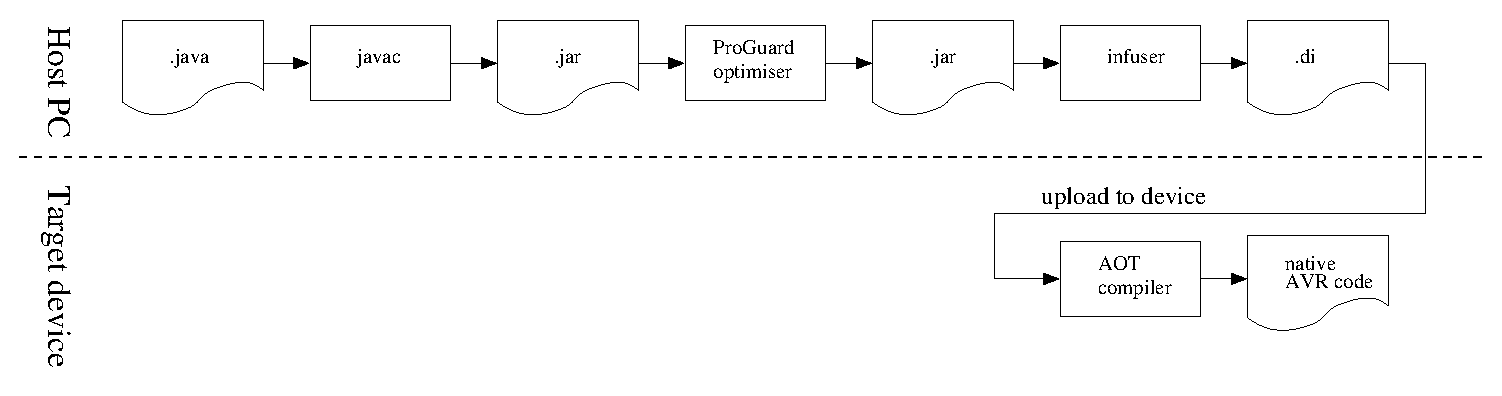
\includegraphics[width=\linewidth]{compilation-process.eps}
\caption{Java source to native AVR code compilation}
\label{fig-translation-process}
\end{figure}

The complete process from Java source to native code on the node is shown in Figure \ref{fig-translation-process}. Like all sensor node JVMs, CapeVM uses a modified JVM bytecode. Java source code is first compiled to normal Java classes. We then use ProGuard \cite{proguard} to optimise the bytecode, but these optimisations, while useful, are limited to very basic steps such as dead code removal, overlapping local variable slots where possible, etc.

The optimised Java classes are then transformed into CapeVM's own bytecode format, called an \emph{infusion}. For details of this transformation we refer to the Darjeeling paper \cite{Brouwers:2009cj} and the extensions to Darjeeling's bytecode described in Chapter \ref{sec-optimisations}. Here it is sufficient to note that no knowledge of the target platform is used in this transformation, so the result is still platform independent. This infusion is then sent to the node, where the AOT compiler translates it to native AVR code at load time.

When the node receives a large programme, it should not have to keep multiple messages in memory since this will consume too much memory. CapeVM's AOT compiler allows the bytecode to be translated to native code in a single pass, one instruction at a time. Only some small, fixed-size data structures are kept in memory during the process. A second pass over the generated code then fills in addresses left blank by branch instructions, since the target addresses of forward branches are not known until the target instruction is generated.

Each message, which can be as small as a single bytecode instruction, can be freed immediately after processing. Since messages do need to be processed in the correct order, the actual transmission protocol may still decide to keep more messages in memory to reduce the need for retransmissions in the case of out of order delivery. But the translation process does not require it to do so, and a protocol that values memory usage over retransmissions cost can simply discard out of order messages and request retransmissions when necessary.


\section{Translating bytecode to native code}
\label{sec-basic-translation}

\begin{table}
\caption{Translation of \mycode{ do{A>>>=1;} while(A>B);}}
\label{tbl-basic-translation}
    \scriptsize
    \begin{tabular}{llll} % NO SIMULATION DATA
    \toprule
    Bytecode            & AOT compiler                       & native code & cycles \\
    \midrule
    \midrule
    0: BRTARGET(0)      & \sccomment{record current address} &            & \\
    1: SLOAD\_0         & emit\_LDD(R1,Y+0)                  & LDD R1,Y+0 & 4 \\
                        & emit\_PUSH(R1)                     & PUSH R1    & 4 \\
    2: SCONST\_1        & emit\_LDI(R1,1)                    & LDI R1,1   & 2 \\
                        & emit\_PUSH(R1)                     & MOV R2,R1  & 1 \\
    3: SUSHR            & emit\_POP(R2)                      &            & \\
                        & emit\_POP(R1)                      & POP R1     & 4 \\
                        & emit\_RJMP(+2)                     & RJMP +2    & 2 \\
                        & emit\_LSR(R1)                      & LSR R1     & 2 \\
                        & emit\_DEC(R2)                      & DEC R2     & 2 \\
                        & emit\_BRPL(-2)                     & BRPL -2    & 3 \\
                        & emit\_PUSH(R1)                     &            & \\
    4: SSTORE\_0        & emit\_POP(R1)                      &            & \\
                        & emit\_STD(Y+0,R1)                  & STD Y+0,R1 & 4 \\
    5: SLOAD\_0         & emit\_LDD(R1,Y+0)                  & LDD R1,Y+0 & 4 \\
                        & emit\_PUSH(R1)                     & PUSH R1    & 4 \\
    6: SLOAD\_1         & emit\_LDD(R1,Y+2)                  & LDD R1,Y+2 & 4 \\
                        & emit\_PUSH(R1)                     &            & \\
    7: IF\_SCMPGT(BT:0) & emit\_POP(R1)                      &            & \\
                        & emit\_POP(R2)                      & POP R2     & 4 \\
                        & emit\_CP(R1,R2)                    & CP R1,R2   & 2 \\
                        & emit\_branchtag(GT,0)              & BRGT 0:    & 2 (taken), \\
                        &                                    &            & or 1 (not taken) \\
    \bottomrule
    \end{tabular}
\end{table}

The baseline AOT compiler used in CapeVM is an implementation of Ellul's approach, as described in his thesis \cite{Ellul:2012thesis}, adapted for the Atmel ATmega128 CPU, while Ellul's work uses the Texas Instruments MSP430. 

In this unoptimised version of the translator, each bytecode instruction the VM receives is simply replaced with a fixed, equivalent sequence of native instructions. The native stack is used to mimic the VM's operand stack. An example of this is shown in Table \ref{tbl-basic-translation}.

The first column shows a fragment of bytecode which does a shift right of 16-bit variable \mycode{A}, and repeats this while \mycode{A} is greater than \mycode{B}. While this may not be a very useful operation, it is the smallest example that will allow us to illustrate our code generation optimisations in the following chapter. The second column shows the code the AOT compiler will execute for each bytecode instruction. Together, the first and second column match the case labels and body of a big switch statement in the compiler. The third column shows the resulting AVR native code, which is currently almost a 1-on-1 mapping, with the exception of the branch instruction and some optimisations by a simple peephole optimiser, both described below.

The example has been slightly simplified for readability. Since the AVR is an 8-bit CPU, in the real code many instructions are duplicated for the high and low bytes. The cycle count is based on the actual number of generated instructions, and for a single iteration.


\subsection{Peephole optimisation}
\begin{table}
\caption{CapeVM's peephole optimisations}
\label{tbl-CapeVM-peephole}
    \begin{threeparttable}
    \begin{tabular}{lrrlrr} % NO SIMULATION DATA
    \toprule
    Before         & Cycles & Bytes   & After        & Cycles & Bytes   \\
    Instructions   &        &         & Instructions &        &         \\
    \midrule
    \midrule
    PUSH Rx        & 4      & 4       &              & 0      & 0 \\
    POP Rx         &        &         &              &        & \\
    \midrule
    PUSH Rx        & 4      & 4       & MOV Ry, Rx   & 1      & 2 \\
    POP Ry         &        &         &              &        & \\
    \midrule
    ST X+, Rx      & 4      & 4       &              & 0      & 0 \\
    LD -X, Rx      &        &         &              &        & \\
    \midrule
    ST X+, Rx      & 4      & 4       & MOV Ry, Rx   & 1      & 2 \\
    LD -X, Ry      &        &         &              &        & \\
    \midrule
    MOV Ry, Rx     & 2      & 4       & MOVW Ry, Rx  & 1      & 2 \\
    MOV Ry+1, Rx+1 &        &         &              &        & \\
    \bottomrule
    \end{tabular}
    \begin{tablenotes}
    \item The X register is used as the reference stack pointer.
    \end{tablenotes}
    \end{threeparttable}
\end{table}

Since the baseline should be as close as possible to Ellul's implementation, a similar set of peephole optimisations were implemented. However, differences between the ATmega and MSP430 instruction sets means they are not completely identical. The complete set of peephole optimisations in CapeVM is shown in Table \ref{tbl-CapeVM-peephole}.

A \mycode{push} directly followed by a \mycode{pop} are both either eliminated or replaced by a \mycode{mov}. A push or pop may be either a real \mycode{push} or \mycode{pop} instruction for the integer stack, or implemented using a \mycode[c-objdump]{st X+} or \mycode[c-objdump]{ld -X} instruction for the reference stack. Both cases are optimised in the same way. We also similarly optimise blocks of pushes followed by blocks of pops, which are very common on the 8-bit ATmega. 

When blocks of push and pop instructions target different registers, this results in multiple \mycode{mov} instructions. Two \mycode{mov} instructions with consecutive registers can be further optimised using the \mycode{movw} instruction to copy a register pair to another register pair in a single cycle.


\subsection{Branches}
Forward branches pose a problem for this direct translation approach since the target address is not yet known. A second problem is that on the ATmega, a branch may take 1 to 3 words, depending on the distance to the target, so it is also not known how much space should be reserved for a branch.

To solve this, the infuser modifies the bytecode by inserting a new instruction, \mycode{BRTARGET}, in front of any instruction that is the target of a branch. The branch instructions themselves are modified to target the id of a \mycode{BRTARGET}, which are implicitly numbered, instead of a bytecode offset. When the VM encounters a \mycode{BRTARGET} during translation, no code is emitted, but the address where the next instruction will be emitted is recorded in a separate part of flash memory. Branch instruction initially emit a temporary 3-word 'branch tag', containing the branch target id and the branch condition. After code generation is finished and all target addresses are known, the VM scans the generated code a second time, and replaces each branch tag with the real branch instruction.

There is still the matter of the different sizes a branch may take. The VM could simply add \mycode{NOP} instructions to smaller branches to keep the size of each branch at 3 words, but this causes both a code size penalty and a performance penalty on small, non-taken branches. Instead, the VM does another scan of the code, before replacing the branch tags, to update the branch target addresses by compensating for cases where a smaller branch will be used. This second scan adds about 500 bytes to the VM, but improves performance, especially on benchmarks where branches are common.

This is an example of something we often see: an optimisation may take a few hundred bytes to implement, but its usefulness may depend on the characteristics of the code being run. In this work we usually decided to implement these optimisations, since in many cases, including this one, they also result in smaller generated code.


\subsection{Safety checks}
CapeVM provides a safe execution environment by adding a number of safety checks, described in Chapter \ref{sec-safety}. An advantage of using a VM to provide safety is that bytecode is more structured than native code. This simplifies the necessary checks, and allows us to perform most of them at translation time.

For each bytecode instruction, a set of checks is defined to guarantee the generated code cannot violate the safety guarantees by writing or branching to an illegal address, under- or overflowing the stack, etc. Like the translation process, these checks are performed one instruction at a time, and only require minimal state to be maintained as a method is being translated, specifically two bytes to keep track of the operand stack.

Most of these checks are performed at translation time, and the VM will reject the code if any of them fail. For the remaining cases, run-time checks are included in the generated code that allow the VM to terminate any faulty application.


\subsection{Bytecode modification}
\label{sec-vm-design-bytecode-modifications}
We made several modifications to the infuser and introduced new bytecode instructions to support our AOT compiler and improve performance. These changes will be introduced in more detail in the following chapters, but for completeness we also list them here:

\begin{itemize}
    \item The \mycode{BRTARGET} opcode marks targets of branch instructions. All branch instructions are modified to target a \mycode{BRTARGET} id instead of a bytecode offset.
    \item The \mycode{MARKLOOP} opcode marks inner loops and the variables they use.
    \item \mycode{PUTFIELD_A_FIXED} and \mycode{GETFIELD_A_FIXED} are used to access an object's reference fields when the offset is known at compile time. The offset is always known at compile time for integer fields.
    \item The \mycode{SIMUL} opcode does 16x16-bit to 32-bit multiplication.
    \item New \mycode{_CONST} versions of the (variable) bit shift opcodes support shifting by a constant number of bits.
    \item The \mycode{INVOKELIGHT} opcode supports an optimised 'lightweight' way of calling methods.
    \item The \mycode{GETCONSTARRAY} opcodes support reading from arrays of constant data stored in the constant pool.
    \item Array access opcodes use 16-bit instead of 32-bit indexes.
\end{itemize}


\subsection{Separation of integers and references}
\label{sec-darjeeling-split-architecure}

An important feature of Darjeeling, which we have maintained in CapeVM, is its separation of integers and references. When the garbage collector runs, it needs to mark the \emph{root set}: the set of all live, directly reachable objects. This set is then iteratively expanded to include all indirectly reachable objects. For example in Figure \ref{fig-jvm-memory}, only the two objects on the left of the heap are in the root set, two others are also reachable but not in the root set, while the fifth is not reachable and will be freed by the garbage collector.

To mark the root set, the garbage collector needs to determine which local variables, static variables, object fields, and values on the operand stack are references. To do this efficiently, references and integers are separated throughout the VM: the operand stack, instance variables on the heap, class static variables, and local variables in a method's stack frame are all split in a block for integers and one for references, as shown in Figure \ref{fig-object-and-stack-frame-layout}.

In CapeVM's AOT compiler we use the native stack for the VM's integer operand stack, so the integer operand stack is no longer in the method's stack frame, but the reference stack is. This uses less memory than having the integer stack in the stack frame, since we need to reserve space for the maximum stack depth in the frame, which is often much lower for the reference stack than for the integer stack. We use the AVR's X register as an extra stack pointer for the reference stack.

\begin{figure}
\centering
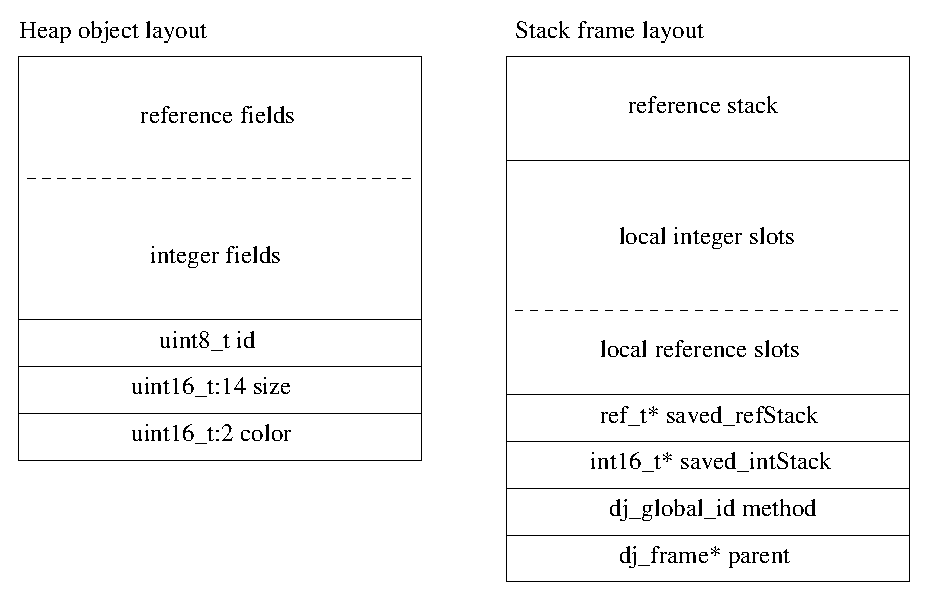
\includegraphics[width=0.8\linewidth]{object-and-stack-frame-layout.eps}
\caption{Infusion, object and stack frame layout}
\label{fig-object-and-stack-frame-layout}
\end{figure}


\section{Limitations}
Since CapeVM is based on Darjeeling, we share its limitations, most notably a lack of floating point support and reflection. In addition, we do not support threads or exceptions because after compilation to native code, we lose the interpreter loop as a convenient place to switch between threads or unwind the stack to jump to an exception handler. Threads and exceptions have been implemented in Ellul's AOT compiler \cite{Ellul:2012thesis}, proving it is possible to add support for both, but we feel the added complexity in an environment where code space is at a premium makes other, more lightweight models for concurrency and error handling more appropriate. Dropping support for threads also allows us to allocate the VM's stack frames on the native stack, which considerably improves performance compared to Darjeeling's approach of allocating stack frames as a linked list on the heap.

We will discuss the cost of using our VM more in more detail in Chapter \ref{sec-evaluation}, and alternatives to some traditional JVM features in Chapter \ref{sec-lessons-from-jvm}.


\section{Target platforms}
CapeVM was implemented for the ATmega128 CPU \cite{Atmel:ATmega128Datasheet}. The AVR family of CPUs is widely used in low power embedded systems and sensor nodes. However, our approach does not depend on any AVR specific properties and we expect similar results for many other CPUs in this class. The main requirements are the ability to reprogramme its own programme memory, and the availability of a sufficient number of registers.

The ATmega128 has 32 8-bit registers. We expect the Cortex M0 \cite{ARM:2009vz}, with 13 32-bit general purpose registers, or the MSP430 \cite{TexasInstrumentsIncorporated:MSP430F1611Datasheet}, with 12 16-bit registers, and used by Ellul and Martinez \cite{Ellul:2010iw}, to both be good matches as well. Section \ref{sec-evaluation-other-platforms} will examine the expected impact of the number of registers and of using a 16-bit or 32-bit architecture on the resulting performance.

\chapter{Optimisations}
\label{sec-optimisations}
Having introduced our baseline AOT compiler, this chapter we will propose several optimisations to improve its performance and reduce the size of the generated code. We will first analyse the difference sources of overhead, and discuss how to reduce each of them.


\section{Sources of overhead}
The performance and code size of the baseline approach still suffers from a large overhead compared to optimised native C. To improve on this, it is important to identify the causes of this overhead. The main sources of overhead we found are:
\begin{itemize}
	\item Lack of optimisations in the Java compiler
	\item AOT code generation overhead
	\begin{itemize}
		\item Push/pop overhead
		\item Load/store overhead
		\item JVM instruction set limitations
	\end{itemize}
	\item Method call overhead
\end{itemize}

We will briefly discuss each source below, before introducing optimisations to reduce it.

\subsection{Lack of optimisation in \mycode{javac}}
A first source of overhead comes from the fact that the standard \mycode{javac} compiler does almost no optimisations.  Since the JVM is an abstract machine, there is no clear performance model to optimise for. Run-time performance depends greatly on the target platform and the VM implementation running the bytecode, which are unknown when compiling Java source code to JVM bytecode. The \mycode{javac} compiler simply compiles the code 'as is'. For example, the loop 

\centerline{\mycode{while (a < b*c) { a*=2; }}}

\noindent will evaluate '\mycode{b*c}' on each iteration, while it is clear that the result will be the same every time.

In most environments this is not a problem because the bytecode is usually compiled to native code before execution, and using knowledge of the target platform and the run-time behaviour, a desktop JIT compiler can make much better decisions than \mycode{javac}. However, since our AOT compiler simply replaces each instruction with a native equivalent, this leads to significant overhead in our VM.

We do use the ProGuard optimiser \cite{proguard}, but this only does very basic optimisations such as method inlining and dead code removal, and does not cover cases such as the example above.

\subsection{AOT translation overhead}
\label{sec-overhead-aot-translation}
Assuming we have high quality JVM bytecode, a second source of overhead comes from the way the bytecode is translated to native code. We distinguish three main types of translation overhead, where the first two are a direct result of the JVM's stack-based architecture.

\subsubsection{Type 1: Pushing and popping values} The compilation process initially results in a large number of push and pop instructions. In our simple example in Table \ref{tbl-basic-translation}, the peephole optimiser was able to eliminate some, but two push/pop pairs remain. For more complex expressions this type of overhead is higher, since more values will be on the stack at the same time. This means more corresponding push and pop instructions will not be consecutive, and the baseline peephole optimiser cannot eliminate these cases.

\subsubsection{Type 2: Loading and storing values} The second type is also due to the JVM's stack-based architecture. Each operation consumes its operands from the stack, but in many cases the same value is needed again soon after. Because the value is no longer on the stack, this results in another load from memory.

In Table \ref{tbl-basic-translation}, it is clear that the \mycode{LDD} instruction at label 5 is unnecessary since the value is already in R1.

\subsubsection{Type 3: JVM instruction set limitations} A third source of overhead due to the baseline AOT compilation process comes from optimisations that are done in native code, but are not possible in JVM bytecode, at least not in our resource-constrained environment.

The JVM instruction set is very simple, which makes it easy to implement, but this also means some things cannot be expressed as efficiently in bytecode as in native code. Given enough processing power, compilers can do the complex transformations necessary to make the compiled JVM code run almost as fast as native C, but a sensor node does not have such resources and must simply execute the instructions as they are.

The code in Table \ref{tbl-basic-translation} does a shift right by one bit. In the JVM instruction set there is no way to express a single bit shift directly. Instead the constant 1 is loaded onto the stack, followed by the generic bit shift instruction. Compare this to addition, where the JVM bytecode does have a special INC instruction to add a constant value to a local variable.

A second example is arrays of constant data. Since the JVM has no concept of constant data, any such data is implemented as a normal array, which has two disadvantages: it will use up precious RAM, and it will be initialised using normal JVM instructions, taking up much more code space than the constant data itself.

\subsection{Method call overhead}
\label{sec-overhead-method-call}
The final source of overhead comes from method calls. In the JVM, each method has a stack frame (or 'activation frame') which the language specification describes as
\begin{quotation}
"containing the target reference (if any) and the argument values (if any), as well as enough space for the local variables and stack for the method to be invoked and any other bookkeeping information that may be required by the implementation (stack pointer, programme counter, reference to previous activation frame, and the like)" \cite{Gosling:2014}
\end{quotation}

CapeVM's stack frame layout was shown in Figure \ref{fig-object-and-stack-frame-layout}. Initialising this complete structure is significantly more work than a native C function call has to do, which may not need a stack frame at all if all the work can be done in registers. Below we list the steps CapeVM goes through to invoke a Java method:

\begin{enumerate}
  \small
  \item Flush the stack cache so parameters are in memory and clear value tags (see sections \ref{sec-optimisations-simple-stack-caching} and \ref{sec-optimisations-popped-value-caching}).
  \item Save the integer and reference stack pointers (SP and X).
  \item Call the VM's \mycode{callMethod} function, which will:
  \begin{enumerate}
    \item allocate memory for the callee's frame
    \item initialise the callee's frame
    \item pass parameters: pop them off the caller's stack and copy them into the callee's locals
    \item activate the callee's frame: set the VM's active frame pointer to the callee
    \item lookup the address of the AOT compiled code
    \item do the actual \mycode{CALL}, which will return any return value in registers R22 and higher
    \item reactivate the old frame: set the VM's active frame pointer back to the caller
    \item return to the caller's AOT compiled code the return value (if any) in R22 and higher
  \end{enumerate}
  \item Restore stack pointer and X register.
  \item Push the return value onto the stack (using stack caching this will be free).
\end{enumerate}

Even after considerable effort optimising this process, this requires roughly 540 cycles for the simplest case: a call to a static method without any parameters or return value. For a virtual method the cost is higher because we need to look up the right implementation. While we may be able to save some more cycles with an even more rigorous refactoring, it is clear that the number of steps involved will always take considerably more time than a native function call.

\subsection{Optimisations}
\label{sec-optimisations-java-source}
Having identified these sources of overhead, we will use the next three sections to describe the set of optimisations we use to address them. Table \ref{tbl-optimisations-overview} lists each optimisation, and the source of overhead it aims to reduce. The following sections will discuss each optimisation in detail.

\begin{table}
\caption{List of optimisations per overhead source}
\label{tbl-optimisations-overview}
    \begin{tabular}{lll} % NO SIMULATION DATA
    \toprule
    & Source of overhead & Optimisation \\
    \midrule
    \midrule
    Section \ref{sec-optimisations-manual-java-source-optimisation} &
    Lack of optimisations in \mycode{javac}        & $\bullet$ Manual optimisation of Java source code \\

    Section \ref{sec-optimisations-aot-translation-overhead} &
    AOT translation overhead                       & \\
    &\hspace{.5cm} Push/pop overhead                & $\bullet$ Improved peephole optimiser \\
    &                                               & $\bullet$ Stack caching \\
    &\hspace{.5cm} Load/store overhead              & $\bullet$ Popped value caching \\
    &                                               & $\bullet$ Mark loops \\
    &\hspace{.5cm} JVM instruction set limitations  & $\bullet$ Constant bit shift optimisation \\
    &                                               & $\bullet$ \mycode{GET/PUTFIELD_A_FIXED} instructions \\
    &                                               & $\bullet$ \mycode{SIMUL} instruction \\
    &                                               & $\bullet$ 16-bit array indexes \\
    &                                               & $\bullet$ Support for constant arrays \\
    Section \ref{sec-optimisations-method-calls} &
    Method call overhead                           & $\bullet$ Lightweight methods \\
    \bottomrule
    \end{tabular}
\end{table}




\section{Manually optimising the Java source code}
\label{sec-optimisations-manual-java-source-optimisation}
As shown in Section \ref{sec-compilation-process}, our current implementation uses three steps to translate Java source code to Darjeeling bytecode: the standard Java compiler, the ProGuard optimiser, and Darjeeling's infuser. None of these do any complex optimisations. 

In a future version, ProGuard and the infuser should be merged into an 'optimising infuser' which uses all the normal, well-known optimisation techniques to produce better quality bytecode, but at the moment we do not have the resources to build such an optimising infuser.

Since our goal is to find out what level of performance is possible on a sensor node, we manually optimise the Java source to get better quality JVM bytecode from \mycode{javac}. While these changes are not an automatic optimisation we developed, we find it imporant to mention them explicitly and analyse their impact, since many developers may expect many of these to happen automatically, and without this step it would be impossible to reproduce our results.

We have been careful to limit ourselves to 'fair' optimisations, by which we mean optimisations that an optimising infuser could reasonably be expected to do automatically, given some basic, conservative assumptions about the performance model. 

The most common optimisations we performed are:
\begin{itemize}
	\item Store the result of expressions calculated in a loop in a temporary variable, if it is known the result will be the same for each iteration.
	\item Since array and object field access is relatively expensive and not cached by the mark loop optimisation discussed in Section \ref{sec-optimisation-markloops}, prefer to minimise array and object access by using a temporary local variable, if the value may be used again soon.
	\item Manually inlining small methods.
	\item Prefer to use 16-bit variables for array indexes where possible.
	\item Use bit shifts for multiplications by a power of two.
\end{itemize}

We will briefly examine the effect of some 'unfair' optimisations on the CoreMark benchmark in Section \ref{sec-evaluation-coremark}. These are optimisations that the infuser most likely couldn't do automatically, but a developer who's aware of the performance of the VM could easily do manually.

\paragraph{Temporary variables}
The first two optimisations generate extra store instructions, which means they may not always be beneficial if the value is never used again. But a value often only needs to be reused only once for it to be faster to store in a local variable than to calculate it twice. If we use the mark loops optimisation discussed in Section \ref{sec-optimisation-markloops}, in many cases the variable may be stored in registers, making accessing them either very cheap, or free.

\paragraph{Manual inlining}
We manually inline all small methods that were either a \mycode{\#define} in the C version of our benchmarks, or a function that was inlined by \mycode{avr-gcc}. ProGuard can also inline small methods, but when it does, it simply replaces the \mycode{INVOKE} instruction with the callee's body, prepended with \mycode{STORE} instructions to pop the parameters off the stack and initialise the callee's local variables. Manual inlining often results in better code, because it may not be necessary to store the parameters if they are only used once. Again, it is easy to imagine that an optimising compiler should be able to come to the same result automaticallly.

\paragraph{Platform independence}
Assuming an optimising infuser does raise the question how platform independent the resulting code is. If the infuser has more specific knowledge about the target platform, it can produce better code for that platform, but, while it should still run anywhere, this may not be as efficient on other platforms.

However, the optimisations described here are only based on very conservative assumptions, and would work well for most devices in this class.

\paragraph{Example} An example of these manual optimisations, applied to the bubble sort benchmark, can be seen in Listing \ref{lst-manual-optimisation}. To have a fair comparison, we applied exactly the same optimisations to the C versions of our benchmarks, but here this had little or no effect on the performance.

\begin{listing}
\centering

\begin{minipage}[t]{0.47\textwidth}
\centering
  \begin{minted}{java}
// ORIGINAL
public static void bsort(int[] numbers)
{
  short NUMBERS=(short)numbers.length;
  for (short i=0; i<NUMBERS; i++)
  {
    for (short j=0; j<NUMBERS-i-1; j++)
    {
      if (numbers[j]>numbers[j+1])
      {
        int temp = numbers[j];
        numbers[j] = numbers[j+1];
        numbers[j+1] = temp;
      }
    }
  }
}
\end{minted}
\end{minipage}
\hfill
\begin{minipage}[t]{0.52\textwidth}
\centering
\begin{minted}[linenos=false]{java}
// MANUALLY OPTIMISED
public static void bsort(int[] numbers)
{
  short NUMBERS=(short)numbers.length;
  for (short i=0; i<NUMBERS; i++)
  {
    short x=(short)(NUMBERS-i-1);
    short j_plus_1 = 1;
    for (short j=0; j<x; j++)
    {
      int val_at_j = numbers[j];
      int val_at_j_plus_1 = numbers[j_plus_1];
      if (val_at_j>val_at_j_plus_1)
      {
        numbers[j] = val_at_j_plus_1;
        numbers[j_plus_1] = val_at_j;
      }
      j_plus_1++;
    }
  }
}
\end{minted}
\end{minipage}
\caption{Optimisation of the bubble sort benchmark}
\label{lst-manual-optimisation}
\end{listing}



\section{AOT translation overhead}
\label{sec-optimisations-aot-translation-overhead}
Now that we have good quality bytecode to work with, we can start addressing the overhead incurred during the AOT compilation process.

\subsection{Improving the peephole optimiser}
\label{sec-improved-peephole}
\begin{table}[hbt]
\centering
\caption{Improved peephole optimiser}
\label{tbl-improved-peephole}
\scriptsize
\addtolength{\tabcolsep}{-2pt}
\begin{tabular}{llll}
\toprule
JVM & AOT compiler & AVR & cycles \\
\hline
0: BRTARGET(0)   & \sccomment{record current addr} &                &   \\
1: SLOAD\_0      & emit\_LDD(R1,Y+0)        & LDD R1,Y+0     & 4 \\
                 & emit\_PUSH(R1)           & PUSH R1        & 4 \\
2: SCONST\_1     & emit\_LDI(R1,1)          & LDI R1,1       & 2 \\
                 & emit\_PUSH(R1)           & MOV R2,R1      & 1 \\
3: SUSHR         & emit\_POP(R2)            &                &   \\
                 & emit\_POP(R1)            & POP R1         & 4 \\
                 & emit\_RJMP(+2)           & RJMP +2        & 2 \\
                 & emit\_LSR(R1)            & LSR R1         & 2 \\
                 & emit\_DEC(R2)            & DEC R2         & 2 \\
                 & emit\_BRPL(-2)           & BRPL -2        & 3 \\
                 & emit\_PUSH(R1)           &                &   \\
4: SSTORE\_0     & emit\_POP(R1)            &                &   \\
                 & emit\_STD(Y+0,R1)        & STD Y+0,R1     & 4 \\
5: SLOAD\_0      & emit\_LDD(R1,Y+0)        & LDD R1,Y+0     & 4 \\
                 & emit\_PUSH(R1)           & MOV R2, R1     & 1 \\
6: SLOAD\_1      & emit\_LDD(R1,Y+2)        & LDD R1,Y+2     & 4 \\
                 & emit\_PUSH(R1)           &                &   \\
7: IF\_SCMPGT 0: & emit\_POP(R1)            &                &   \\
                 & emit\_POP(R2)            &                &   \\
                 & emit\_CP(R1,R2)          & CP R1,R2       & 2 \\
                 & emit\_branchtag(GT,0)    & BRGT 0:        & 2 (taken), \\
                 &                          &                & or 1 (not taken) \\
\bottomrule
\end{tabular}
\end{table}

Our first optimisation is a small but effective extension to the simple peephole optimiser. Instead of optimising only consecutive push/pop pairs, we can optimise any pair of push/pop instructions if the following holds for the instructions in between:
%\begin{itemize}
%   \item they contain the same number of \mycode{push} and \mycode{pop} instructions (the \mycode{pop} matches the \mycode{push})
%   \item they contain no branches
%   \item they may be do not use the \emph{target} register of the \mycode{pop}
%\end{itemize}

\begin{listing}
    \begin{minted}{asm}
    PUSH Rs
    ..
    ..       instructions in between: - contain the same number of push and pop instr.
    ..                                - contain no branches
    ..                                - do not use register Rd
    ..
    POP  Rd
     \end{minted}
\end{listing}

In this case the pair can be eliminated if \mycode{Rs} == \mycode{Rd}, otherwise it is replaced by a '\mycode{mov Rd, Rs}'. Two push/pop pairs remained in our earlier example Table \ref{tbl-basic-translation}. For the pair in instructions 5 and 7, the value is popped into register R2. Since instruction 6 does not use register R2, we can safely replace this pair with a direct move. In contrast, the pair in instructions 1 and 3 cannot be optimised since the value is popped into register R1, which is also used by instruction 2. The result is shown in Table \ref{tbl-improved-peephole}

% This optimisation adds 278 bytes to the optimiser, since it now needs to understand the bytecode well enough to determine which registers are being used.

\subsection{Simple stack caching}
\label{sec-optimisations-simple-stack-caching}
\begin{table}
\caption{Stack caching}
\label{tbl-simplestackcaching}
    \scriptsize\centerline{
    \begin{tabular}{llll|c|c|c|c} % NO SIMULATION DATA
    \toprule
                       &                                                      &                     &        & \multicolumn{4}{c}{cache state} \\
    Bytecode           & AOT compiler                                         & native code         & cycles & R1                   & R2                   & R3                   & R4                   \\
    \midrule
    \midrule
    0: BRTARGET(0)     & \sccomment{record current address}                   &                     &        & \sce{    }{   }{   } & \sce{    }{   }{   } & \sce{    }{   }{   } & \sce{    }{   }{   } \\
    1: SLOAD\_0        & operand\_1 = sc\_getfreereg()                        &                     &        & \sce{\use}{   }{   } & \sce{    }{   }{   } & \sce{    }{   }{   } & \sce{    }{   }{   } \\
                       & emit\_LDD(operand\_1,Y+0)                            & LDD R1,Y+0          &      4 & \sce{\use}{   }{   } & \sce{    }{   }{   } & \sce{    }{   }{   } & \sce{    }{   }{   } \\
                       & sc\_push(operand\_1)                                 &                     &        & \sce{Int1}{   }{   } & \sce{    }{   }{   } & \sce{    }{   }{   } & \sce{    }{   }{   } \\
    2: SCONST\_1       & operand\_1 = sc\_getfreereg()                        &                     &        & \sce{Int1}{   }{   } & \sce{\use}{   }{   } & \sce{    }{   }{   } & \sce{    }{   }{   } \\
                       & emit\_LDI(operand\_1,1)                              & LDI R2,1            &      2 & \sce{Int1}{   }{   } & \sce{\use}{   }{   } & \sce{    }{   }{   } & \sce{    }{   }{   } \\
                       & sc\_push(operand\_1)                                 &                     &        & \sce{Int2}{   }{   } & \sce{Int1}{   }{   } & \sce{    }{   }{   } & \sce{    }{   }{   } \\
    3: SUSHR           & operand\_1 = sc\_pop()                               &                     &        & \sce{Int1}{   }{   } & \sce{\use}{   }{   } & \sce{    }{   }{   } & \sce{    }{   }{   } \\
                       & operand\_2 = sc\_pop()                               &                     &        & \sce{\use}{   }{   } & \sce{\use}{   }{   } & \sce{    }{   }{   } & \sce{    }{   }{   } \\
                       & emit\_JMP(+2)                                        & JMP +2              &      2 & \sce{\use}{   }{   } & \sce{\use}{   }{   } & \sce{    }{   }{   } & \sce{    }{   }{   } \\
                       & emit\_LSR(operand\_2)                                & LSR R1              &      2 & \sce{\use}{   }{   } & \sce{\use}{   }{   } & \sce{    }{   }{   } & \sce{    }{   }{   } \\
                       & emit\_DEC(operand\_1)                                & DEC R2              &      1 & \sce{\use}{   }{   } & \sce{\use}{   }{   } & \sce{    }{   }{   } & \sce{    }{   }{   } \\
                       & emit\_BRPL(-2)                                       & BRPL -2             &      1 & \sce{\use}{   }{   } & \sce{\use}{   }{   } & \sce{    }{   }{   } & \sce{    }{   }{   } \\
                       & sc\_push(operand\_2)                                 &                     &        & \sce{Int1}{   }{   } & \sce{\use}{   }{   } & \sce{    }{   }{   } & \sce{    }{   }{   } \\
    4: SSTORE\_0       & operand\_1 = sc\_pop()                               &                     &        & \sce{\use}{   }{   } & \sce{    }{   }{   } & \sce{    }{   }{   } & \sce{    }{   }{   } \\
                       & emit\_STD(Y+0,operand\_1)                            & STD Y+0,R1          &      4 & \sce{\use}{   }{   } & \sce{    }{   }{   } & \sce{    }{   }{   } & \sce{    }{   }{   } \\
    5: SLOAD\_0        & operand\_1 = sc\_getfreereg()                        &                     &        & \sce{\use}{   }{   } & \sce{    }{   }{   } & \sce{    }{   }{   } & \sce{    }{   }{   } \\
                       & emit\_LDD(operand\_1,Y+0)                            & LDD R1,Y+0          &      4 & \sce{\use}{   }{   } & \sce{    }{   }{   } & \sce{    }{   }{   } & \sce{    }{   }{   } \\
                       & sc\_push(operand\_1)                                 &                     &        & \sce{Int1}{   }{   } & \sce{    }{   }{   } & \sce{    }{   }{   } & \sce{    }{   }{   } \\
    6: SLOAD\_1        & operand\_1 = sc\_getfreereg()                        &                     &        & \sce{Int1}{   }{   } & \sce{\use}{   }{   } & \sce{    }{   }{   } & \sce{    }{   }{   } \\
                       & emit\_LDD(operand\_1,Y+2)                            & LDD R2,Y+2          &      4 & \sce{Int1}{   }{   } & \sce{\use}{   }{   } & \sce{    }{   }{   } & \sce{    }{   }{   } \\
                       & sc\_push(operand\_1)                                 &                     &        & \sce{Int2}{   }{   } & \sce{Int1}{   }{   } & \sce{    }{   }{   } & \sce{    }{   }{   } \\
    7: IF\_SCMPGT(BT:0)& operand\_1 = sc\_pop()                               &                     &        & \sce{Int1}{   }{   } & \sce{\use}{   }{   } & \sce{    }{   }{   } & \sce{    }{   }{   } \\
                       & operand\_2 = sc\_pop()                               &                     &        & \sce{\use}{   }{   } & \sce{\use}{   }{   } & \sce{    }{   }{   } & \sce{    }{   }{   } \\
                       & emit\_CP(operand\_1, operand\_2);                    & CP R2,R1            &      2 & \sce{\use}{   }{   } & \sce{\use}{   }{   } & \sce{    }{   }{   } & \sce{    }{   }{   } \\
                       & emit\_branchtag(GT, 0);                              & BRGT 0:             &      2 & \sce{\use}{   }{   } & \sce{\use}{   }{   } & \sce{    }{   }{   } & \sce{    }{   }{   } \\
    \bottomrule
    \end{tabular}
    }
\end{table}


The improved peephole optimiser can remove part of the type 1 overhead, but still many cases remain where it cannot eliminate the push/pop instructions. We use a form of stack caching \cite{Ertl:1995dv} to eliminate most of the remaining push/pop overhead. Stack caching is not a new technique, originally proposed for Forth interpreters in 1995. But the tradeoffs involved are very different depending on the scenario it is applied in, and it turns out to be exceptionally well suited for a sensor node AOT compiler:

First, the VM in the original paper is an interpreter, which means the stack cache has to be very lightweight, or the overhead from managing it at run time will outweigh the time saved by reducing memory accesses. Since we only need to keep track of the cache state at translation time, this restriction does not apply for an AOT compiler and we can afford to spend more time managing it. Second, the simplicity of the approach means it requires very little memory: only 11 bytes of RAM and less than 1KB of code more than the peephole optimiser.

The basic idea of stack caching is to keep the top elements of the stack in registers instead of main memory. We add a cache state to our VM to keep track of which registers are holding stack elements. For example, if the top two elements are kept in registers, an ADD instruction does not need to access main memory, but can simply add these registers, and update the cache state. Values are only spilled to memory when all registers available for stack caching are in use.

In the baseline AOT approach, each JVM instruction maps to a fixed sequence of native instructions that always use the same registers. Using stack caching, the registers are controlled by a stack cache manager that provides three functions:
\begin{itemize}
    \item \mycode{getfree}: Instructions such as load instructions will need a free register to load the value into, which will later be pushed onto the stack. If all registers are in use, \mycode{getfree} spills the register that's lowest on the stack to memory by emitting a \mycode{PUSH}, and then returns that register. This way the top of the stack is kept in registers, while lower elements may be spilled to memory.
    \item \mycode{pop}: Pops the top element off the stack and tells the code generator in which register to find it. If stack elements have previously been spilled to main memory and no  elements are left in registers, \mycode{pop} will emit a real \mycode{POP} instruction to get the value back from memory.
    \item \mycode{push}: Updates the cache state so the passed register is now at the top of the stack. This should be a register that was previously returned by \mycode{getfree}, or \mycode{pop}.
\end{itemize}

Using stack caching, code generation is split between the instruction translator, which emits the instructions that do the actual work, and the cache manager which manages the registers and may emit code to spill stack elements to memory, or to retrieve them again. But as long as enough registers are available, it will only manipulate the cache state.

In Table \ref{tbl-simplestackcaching} we translate the same example we used before, but this time using stack caching. The \mycode{emit\_PUSH} and \mycode{emit\_POP} instructions have been replaced by calls to the cache manager, and instructions that load something onto the stack start by asking the cache manager for a free register. The state of the stack cache is shown in the three columns added to the right. Currently it only tracks whether a register is on the stack or not. "Int1" marks the top element, followed by "Int2", etc. This example does not use the reference stack, but it is cache in the same way as the integer stack. In the next two optimisations we will extend the cache state further.
 
The example only shows three registers, but the ATmega128 we use has 32 8-bit registers. Since Darjeeling uses a 16-bit stack, we manage them as pairs. 10 registers are reserved, for example as a scratch register or to store a pointer to local or static variables, leaving 11 pairs available for stack caching.

\paragraph{Branches} Branch targets may be reached from multiple locations. We know the cache state if it was reached from the previous instruction, but not if it was reached through a branch. To ensure the cache state is the same on both paths, we flush the whole stack to memory whenever we encounter either a branch or a \mycode{BRTARGET} instruction. 

This may seem bad for performance, but fortunately in the code generated by \mycode{javac} the stack is empty at almost all branches. The exception is the ternary \mycode{?} \mycode{:} operator, which may cause a conditional branch with elements on the stack, but in most cases flushing at branches and branch targets does not result in any extra overhead.

\subsection{Popped value caching}
\label{sec-optimisations-popped-value-caching}
Stack caching can eliminate most of the push/pop overhead, even when the stack depth increases. We now turn our attention to reducing the overhead resulting from load and store instructions.

\begin{table*}[hbt]
\centering
\caption{Popped value caching}
\label{tbl-poppedvaluecaching}
\scriptsize
\addtolength{\tabcolsep}{-2pt}
\begin{tabular}{llll|c|c|c|c}
\toprule
JVM                & AOT compiler                                         & AVR                 & cycles & cache state R1       & cache state R2       & cache state R3       & cache state R4       \\
\hline
0: BRTARGET(0)     & \sccomment{record current address}                   &                     &        & \sce{    }{   }{   } & \sce{    }{   }{   } & \sce{    }{   }{   } & \sce{    }{   }{   } \\
1: SLOAD\_0        & operand\_1 = sc\_getfreereg()                        &                     &        & \sce{\use}{   }{   } & \sce{    }{   }{   } & \sce{    }{   }{   } & \sce{    }{   }{   } \\
                   & emit\_LDD(operand\_1,Y+0)                            & LDD R1,Y+0          & 4      & \sce{\use}{   }{   } & \sce{    }{   }{   } & \sce{    }{   }{   } & \sce{    }{   }{   } \\
                   & sc\_push(operand\_1)                                 &                     &        & \sce{Int1}{LS0}{   } & \sce{    }{   }{   } & \sce{    }{   }{   } & \sce{    }{   }{   } \\
2: SCONST\_1       & operand\_1 = sc\_getfreereg()                        &                     &        & \sce{Int1}{LS0}{   } & \sce{\use}{   }{   } & \sce{    }{   }{   } & \sce{    }{   }{   } \\
                   & emit\_LDI(operand\_1,1)                              & LDI R2,1            & 2      & \sce{Int1}{LS0}{   } & \sce{\use}{   }{   } & \sce{    }{   }{   } & \sce{    }{   }{   } \\
                   & sc\_push(operand\_1)                                 &                     &        & \sce{Int2}{LS0}{   } & \sce{Int1}{CS1}{   } & \sce{    }{   }{   } & \sce{    }{   }{   } \\
3: SUSHR           & operand\_1 = sc\_pop\_destructive()                  &                     &        & \sce{Int1}{LS0}{   } & \sce{\use}{   }{   } & \sce{    }{   }{   } & \sce{    }{   }{   } \\
                   & operand\_2 = sc\_pop\_destructive()                  &                     &        & \sce{\use}{   }{   } & \sce{\use}{   }{   } & \sce{    }{   }{   } & \sce{    }{   }{   } \\
                   & emit\_JMP(+2)                                        & JMP +2              & 2      & \sce{\use}{   }{   } & \sce{\use}{   }{   } & \sce{    }{   }{   } & \sce{    }{   }{   } \\
                   & emit\_LSR(operand\_2)                                & LSR R1              & 2      & \sce{\use}{   }{   } & \sce{\use}{   }{   } & \sce{    }{   }{   } & \sce{    }{   }{   } \\
                   & emit\_DEC(operand\_1)                                & DEC R2              & 1      & \sce{\use}{   }{   } & \sce{\use}{   }{   } & \sce{    }{   }{   } & \sce{    }{   }{   } \\
                   & emit\_BRPL(-2)                                       & BRPL -2             & 1      & \sce{\use}{   }{   } & \sce{\use}{   }{   } & \sce{    }{   }{   } & \sce{    }{   }{   } \\
                   & sc\_push(operand\_2)                                 &                     &        & \sce{\use}{   }{   } & \sce{Int1}{   }{   } & \sce{    }{   }{   } & \sce{    }{   }{   } \\
4: SSTORE\_0       & operand\_1 = sc\_pop\_tostore()                      &                     &        & \sce{    }{   }{   } & \sce{\use}{LS0}{   } & \sce{    }{   }{   } & \sce{    }{   }{   } \\
                   & emit\_STD(Y+0,operand\_1)                            & STD Y+0,R2          & 4      & \sce{    }{   }{   } & \sce{\use}{LS0}{   } & \sce{    }{   }{   } & \sce{    }{   }{   } \\
5: SLOAD\_0        & \sccomment{skip codegen, update cache state}         &                     &        & \sce{    }{   }{   } & \sce{Int1}{LS0}{   } & \sce{    }{   }{   } & \sce{    }{   }{   } \\
6: SLOAD\_1        & operand\_1 = sc\_getfreereg()                        &                     &        & \sce{\use}{   }{   } & \sce{Int1}{LS0}{   } & \sce{    }{   }{   } & \sce{    }{   }{   } \\
                   & emit\_LDD(operand\_1,Y+2)                            & LDD R1,Y+2          & 4      & \sce{\use}{   }{   } & \sce{Int1}{LS0}{   } & \sce{    }{   }{   } & \sce{    }{   }{   } \\
                   & sc\_push(operand\_1)                                 &                     &        & \sce{Int1}{LS1}{   } & \sce{Int2}{LS0}{   } & \sce{    }{   }{   } & \sce{    }{   }{   } \\
7: IF\_SCMPGT 0:   & operand\_1 = sc\_pop\_nondestructive()               &                     &        & \sce{\use}{LS1}{   } & \sce{Int1}{LS0}{   } & \sce{    }{   }{   } & \sce{    }{   }{   } \\
                   & operand\_2 = sc\_pop\_nondestructive()               &                     &        & \sce{\use}{LS1}{   } & \sce{\use}{LS0}{   } & \sce{    }{   }{   } & \sce{    }{   }{   } \\
                   & emit\_CP(operand\_1, operand\_2);                    & CP R1,R2            & 2      & \sce{\use}{LS1}{   } & \sce{\use}{LS0}{   } & \sce{    }{   }{   } & \sce{    }{   }{   } \\
                   & emit\_branchtag(GT, 0);                              & BRGT 0:             & 2      & \sce{\use}{LS1}{   } & \sce{\use}{LS0}{   } & \sce{    }{   }{   } & \sce{    }{   }{   } \\
\bottomrule
\end{tabular}
\addtolength{\tabcolsep}{2pt}
\end{table*}



We add a 'value tag' to each register's cache state to keep track of what value is currently held in the register, even after it is popped from the stack. Some JVM instructions have a value tag associated with them to indicate which value or variable they load, store, or modify. Each tag consist of a tuple (type, datatype, number). For example, the JVM instructions \mycode{ILOAD\_0} and \mycode{ISTORE\_0}, which load and store the local integer variable with id 0, both have tag LI0, short for (local, int, 0). \mycode{SCONST\_1} has tag CS1, or (constant, short, 1), etc. These tags are encoded in a 16-bit value.

The cache manager is extended with a \mycode{sc\_can\_skip} function. This function will examine the type of each instruction, its value tag, and the cache state. If it finds that we are loading a value that is already present in a register, it updates the cache state to put that register on the stack, and returns true to tell the main loop to skip code generation for this instruction.

Table \ref{tbl-poppedvaluecaching} shows popped value caching applied to our example. At first, the stack is empty. When \mycode{sc\_push} is called, it detects the current instruction's value tag, and marks the fact that R1 now contains LS0. In \mycode{SUSHR\_CONST}, the \mycode{pop} has been changed to \mycode{pop\_destructive}. This tells the cache manager that the value in the register will be destroyed, so the value tag has to be cleared again since R1 will no longer contain LS0. The \mycode{SSTORE\_0} instruction now calls \mycode{pop\_tostore} instead of  \mycode{pop}, to inform the cache manager it will store this value in the variable identified by \mycode{SSTORE\_0}'s value tag. This means the register once again contains LS0. If any other register was marked as containing LS0, the cache manager would clear that tag, since it is no longer accurate after we update the variable.

In line 5, we need to load LS0 again, but now the cache state shows that LS0 is already in R1. This means we do not need to load it from memory, but just update the cache state so that R1 is pushed onto the stack. At run time this \mycode{SLOAD\_0} will have no cost at all.

There are a few more details to get right. For example if we load a value that's already on the stack, we generate a move to copy it. When \mycode{sc\_getfree} is called, it will try to return a register without a value tag. If none are available, the least recently used register is returned. This is done to maximise the chance we can reuse a value later, since recently used values are more likely to be used again.

\paragraph{Branches} As we do not know the state of the registers if an instruction is reached through a branch, we have to clear all value tags when we pass a \mycode{BRTARGET} instruction, meaning that any new loads will have to come from memory. At branches we can keep the value tags, because if the branch is not taken, we do know the state of the registers in the next instruction.

\subsection{Mark loops}
\label{sec-optimisation-markloops}
\begin{table}
\caption{Mark loops}
\label{tbl-markloop}
    \begin{tabular}{llll|c|c|c|c}
    \toprule
    JVM                & AOT compiler                                         & AVR                 & cycles & cache state R1       & cache state R2       & cache state R3       & cache state R4       \\
    \midrule
    \midrule
    0: MARKLOOP(0,1)   & \sccomment{emit markloop prologue:}                  & LDD R1,Y+0          & 4      & \sce{    }{LS0}{PIN} & \sce{    }{   }{   } & \sce{    }{   }{   } & \sce{    }{   }{   } \\
                       & \sccomment{LS0 and LS1 are live}                     & LDD R2,Y+2          & 4      & \sce{    }{LS0}{PIN} & \sce{    }{LS1}{PIN} & \sce{    }{   }{   } & \sce{    }{   }{   } \\
    1: BRTARGET(0)     & \sccomment{record current address}                   &                     &        & \sce{    }{LS0}{PIN} & \sce{    }{LS1}{PIN} & \sce{    }{   }{   } & \sce{    }{   }{   } \\
    2: SLOAD\_0        & \sccomment{skip codegen, update cache state}         &                     &        & \sce{Int1}{LS0}{PIN} & \sce{    }{LS1}{PIN} & \sce{    }{   }{   } & \sce{    }{   }{   } \\
    3: SCONST\_1       & operand\_1 = sc\_getfreereg()                        &                     &        & \sce{Int1}{LS0}{PIN} & \sce{    }{LS1}{PIN} & \sce{\use}{   }{   } & \sce{    }{   }{   } \\
                       & emit\_LDI(operand\_1,1)                              & LDI R3,1            & 2      & \sce{Int1}{LS0}{PIN} & \sce{    }{LS1}{PIN} & \sce{\use}{   }{   } & \sce{    }{   }{   } \\
                       & sc\_push(operand\_1)                                 &                     &        & \sce{Int2}{LS0}{PIN} & \sce{    }{LS1}{PIN} & \sce{Int1}{CS1}{   } & \sce{    }{   }{   } \\
    4: SUSHR           & operand\_1 = sc\_pop\_destructive()                  &                     &        & \sce{Int1}{LS0}{PIN} & \sce{    }{LS1}{PIN} & \sce{\use}{   }{   } & \sce{    }{   }{   } \\
                       & operand\_2 = sc\_pop\_destructive()                  & MOV R4,R1           & 1      & \sce{    }{LS0}{PIN} & \sce{    }{LS1}{PIN} & \sce{\use}{   }{   } & \sce{\use}{   }{   } \\
                       & emit\_JMP(+2)                                        & JMP +2              & 2      & \sce{    }{LS0}{PIN} & \sce{    }{LS1}{PIN} & \sce{\use}{   }{   } & \sce{\use}{   }{   } \\
                       & emit\_LSR(operand\_2)                                & LSR R4              & 2      & \sce{    }{LS0}{PIN} & \sce{    }{LS1}{PIN} & \sce{\use}{   }{   } & \sce{\use}{   }{   } \\
                       & emit\_DEC(operand\_1)                                & DEC R3              & 1      & \sce{    }{LS0}{PIN} & \sce{    }{LS1}{PIN} & \sce{\use}{   }{   } & \sce{\use}{   }{   } \\
                       & emit\_BRPL(-2)                                       & BRPL -2             & 1      & \sce{    }{LS0}{PIN} & \sce{    }{LS1}{PIN} & \sce{\use}{   }{   } & \sce{\use}{   }{   } \\
                       & sc\_push(operand\_2)                                 &                     &        & \sce{    }{LS0}{PIN} & \sce{    }{LS1}{PIN} & \sce{\use}{   }{   } & \sce{Int1}{   }{   } \\
    5: SSTORE\_0       & \sccomment{emit MOV, update cache state}             & MOV R1,R4           & 1      & \sce{    }{LS0}{PIN} & \sce{    }{LS1}{PIN} & \sce{    }{   }{   } & \sce{    }{   }{   } \\
    6: SLOAD\_0        & \sccomment{skip codegen, update cache state}         &                     &        & \sce{Int1}{LS0}{PIN} & \sce{    }{LS1}{PIN} & \sce{    }{   }{   } & \sce{    }{   }{   } \\
    7: SLOAD\_1        & \sccomment{skip codegen, update cache state}         &                     &        & \sce{Int2}{LS0}{PIN} & \sce{Int1}{LS1}{PIN} & \sce{    }{   }{   } & \sce{    }{   }{   } \\
    8: IF\_SCMPGT(BT:0)& operand\_1 = sc\_pop\_nondestructive()               &                     &        & \sce{Int1}{LS0}{PIN} & \sce{    }{LS1}{PIN} & \sce{    }{   }{   } & \sce{    }{   }{   } \\
                       & operand\_2 = sc\_pop\_nondestructive()               &                     &        & \sce{    }{LS0}{PIN} & \sce{    }{LS1}{PIN} & \sce{    }{   }{   } & \sce{    }{   }{   } \\
                       & emit\_CP(operand\_1, operand\_2);                    & CP R2,R1            & 2      & \sce{    }{LS0}{PIN} & \sce{    }{LS1}{PIN} & \sce{    }{   }{   } & \sce{    }{   }{   } \\
                       & emit\_branchtag(GT, 0);                              & BRGT 1:             & 2      & \sce{    }{LS0}{PIN} & \sce{    }{LS1}{PIN} & \sce{    }{   }{   } & \sce{    }{   }{   } \\
    9: MARKLOOP(end)   & \sccomment{emit markloop epilogue: LS0 is live}      & STD Y+0,R1          & 4      & \sce{    }{LS0}{   } & \sce{    }{LS1}{   } & \sce{    }{   }{   } & \sce{    }{   }{   } \\
    \bottomrule
    \end{tabular}
\end{table}


Popped value caching reduces the type 2 overhead significantly, but the fact that we have to clear the value tags at branch targets means that a large part of that overhead still remains. This is particularly true for loops, since each iteration often uses the same variables, but the branch to start the next iteration clears those values from the stack cache. This is addressed by the next optimisation.

Again, we modify the infuser to add a new instruction to the bytecode: \mycode{MARKLOOP}. This instruction is used to mark the beginning and end of each inner loop. \mycode{MARKLOOP} has a larger payload than most JVM instructions: it contains a list of value tags that will appear in the loop and how often each tag appears, sorted in descending order.

When we encounter the \mycode{MARKLOOP} instruction, the VM may decide to reserve a number of registers and pin the most frequently used local variables to them. If it does, code is generated to prefetch these variables from memory and store them in registers. While in the loop, loading or storing these pinned variables does not require memory access, but only a manipulation of the cache state, and possibly a simple move between registers. However, these registers will no longer be available for normal stack caching. Since 4 register pairs need to be reserved for code generation, at most 7 of the 11 available pairs can be used by mark loops.

Because the only way to enter and leave the loop is through the \mycode{MARKLOOP} instructions, the values can remain pinned for the whole duration of the block, regardless of the branches made inside. This lets us eliminate more load instructions, and also replace store instructions by a much cheaper move to the pinned register. \mycode{INC} instructions, which increment a local variable, operate directly on the pinned register, saving both a load and a store. All these cases are handled in \mycode{sc\_can\_skip}, bypassing the normal code generation. We also need to make a small change to \mycode{sc\_pop\_destructive}. If the register we're about to pop is pinned, we cannot just return it since it would corrupt the value of the pinned local variable. Instead we will first emit a move to a free, non-pinned register, and return that instead.

In Table \ref{tbl-markloop} the first instruction is now \mycode{MARKLOOP}, which tells the compiler local short variables 0 and 1 will be used. The compiler decides to pin them both to registers 1 and 2. The \mycode{MARKLOOP} instruction also tells the VM whether or not the variables are live, which they are at this point, so the two necessary loads are generated. This is reflected in the cache state. No elements are on the stack yet, but register 1 is pinned to LS0, and register 2 to LS1.

Next, LS0 is loaded. Since it is pinned to register 1, no code is generated, but the cache state is updated to reflect LS0 is now on top of the stack. Next, \mycode{SUSHR\_CONST} pops destructively. We cannot simply return register 1 since that would corrupt the value of variable LS0, so \mycode{sc\_pop\_destructive} emits a move to a free register and returns that register instead. Since LS0 is pinned, we can also skip \mycode{SSTORE\_0}, but we do need to emit a move back to the pinned register.

The next two loads are straightforward and can be skipped, and in the branch we see the registers are popped non-destructively, so we can use the pinned registers directly.

Finally, we see the loop ends with another \mycode{MARKLOOP}, telling the compiler only local 0 is live at this point. This means we need to store LS0 in register 1 back to memory, but we can skip LS1 since it is no longer needed.

\subsection{Instruction set modifications}
Next, we introduce four optimisations that target the type 3 overhead: cases where limitations in the JVM instruction set means we cannot express some operations as efficiently as we would like. This type of overhead is the most difficult to address because many of the transformations a desktop VM can do to avoid it take more resources than we can afford on a tiny device. Also, this type of overhead covers many different cases, and optimisations that help in a specific case may not be general enough to justify spending additional resources on it.

Still, there are a few things we can do by modifying the instruction set, that come at little cost to the VM and can make a significant difference.

Darjeeling's original instruction set is already quite different from the normal JVM instruction set. The most important change is the introduction of 16-bit operations. The JVM is internally a 32-bit machine, meaning \mycode{short}, \mycode{byte}, and \mycode{char} are internally stored as 32-bit integers. On a sensor device where memory is the most scarce resource, we often want to use shorter data types. To support this, Darjeeling internally stores values in 16-bit slots, and introduces 16-bit versions of all integer operations. For example if we want to multiply two shorts and store the result in a short, the 32-bit \mycode{IMUL} instruction is replaced by the 16-bit \mycode{SMUL} instruction. These transformations are all done by the infuser (see Figure \ref{fig-translation-process}).

However, the changes made by Darjeeling are primarily aimed at reducing memory consumption, not at improving performance. We extend the infuser to make several other changes. The \mycode{BRTARGET} and \mycode{MARKLOOP} instructions have already been discussed, and the \mycode{INVOKELIGHT} instruction is the topic of the next section. In addition to these, we made the following four other modifications to Darjeeling's instruction set:

\subsubsection{Constant bit shifts}
\label{sec-opt-constant-shift}
\begin{table*}[hbt]
\centering
\caption{Constant bit shift optimisation}
\label{tbl-constshift}
\scriptsize
\addtolength{\tabcolsep}{-2pt}
\begin{tabular}{llll|c|c|c|c}
\toprule
JVM                & AOT compiler                                         & AVR                 & cycles & cache state R1       & cache state R2       & cache state R3       & cache state R4       \\
\hline
0: MARKLOOP(0,1)   & \sccomment{emit markloop prologue:}                  & LDD R1,Y+0          & 4      & \sce{    }{LS0}{PIN} & \sce{    }{   }{   } & \sce{    }{   }{   } & \sce{    }{   }{   } \\
                   & \sccomment{LS0 and LS1 are live}                     & LDD R2,Y+2          & 4      & \sce{    }{LS0}{PIN} & \sce{    }{LS1}{PIN} & \sce{    }{   }{   } & \sce{    }{   }{   } \\
1: BRTARGET(0)     & \sccomment{record current address}                   &                     &        & \sce{    }{LS0}{PIN} & \sce{    }{LS1}{PIN} & \sce{    }{   }{   } & \sce{    }{   }{   } \\
2: SLOAD\_0        & \sccomment{skip codegen, just update cache state}    &                     &        & \sce{Int1}{LS0}{PIN} & \sce{    }{LS1}{PIN} & \sce{    }{   }{   } & \sce{    }{   }{   } \\
3: SUSHR\_CONST(1) & \sccomment{operand\_1 = sc\_pop\_destructive()}      & MOV R3,R1           & 1      & \sce{    }{LS0}{PIN} & \sce{    }{LS1}{PIN} & \sce{\use}{   }{   } & \sce{    }{   }{   } \\
                   & \sccomment{it\_LSR(operand\_1)}                      & LSR R3              & 2      & \sce{    }{LS0}{PIN} & \sce{    }{LS1}{PIN} & \sce{\use}{   }{   } & \sce{    }{   }{   } \\
                   & \sccomment{\_push(operand\_1)}                       &                     &        & \sce{    }{LS0}{PIN} & \sce{    }{LS1}{PIN} & \sce{Int1}{   }{   } & \sce{    }{   }{   } \\
4: SSTORE\_0       & \sccomment{emit MOV, update cache state}             & MOV R1,R3           & 1      & \sce{    }{LS0}{PIN} & \sce{    }{LS1}{PIN} & \sce{    }{   }{   } & \sce{    }{   }{   } \\
5: SLOAD\_0        & \sccomment{skip codegen, just update cache state}    &                     &        & \sce{Int1}{LS0}{PIN} & \sce{    }{LS1}{PIN} & \sce{    }{   }{   } & \sce{    }{   }{   } \\
6: SLOAD\_1        & \sccomment{skip codegen, just update cache state}    &                     &        & \sce{Int2}{LS0}{PIN} & \sce{Int1}{LS1}{PIN} & \sce{    }{   }{   } & \sce{    }{   }{   } \\
7: IF\_SCMPGT(BT:0)& operand\_1 = sc\_pop\_nondestructive()               &                     &        & \sce{Int1}{LS0}{PIN} & \sce{    }{LS1}{PIN} & \sce{    }{   }{   } & \sce{    }{   }{   } \\
                   & operand\_2 = sc\_pop\_nondestructive()               &                     &        & \sce{    }{LS0}{PIN} & \sce{    }{LS1}{PIN} & \sce{    }{   }{   } & \sce{    }{   }{   } \\
                   & emit\_CP(operand\_1, operand\_2);                    & CP R2,R1            & 2      & \sce{    }{LS0}{PIN} & \sce{    }{LS1}{PIN} & \sce{    }{   }{   } & \sce{    }{   }{   } \\
                   & emit\_branchtag(GT, 0);                              & BRGT 1:             & 2      & \sce{    }{LS0}{PIN} & \sce{    }{LS1}{PIN} & \sce{    }{   }{   } & \sce{    }{   }{   } \\
8: MARKLOOP(end)   & \sccomment{emit markloop epilogue: LS0 is live}      & STD Y+0,R1          & 4      & \sce{    }{LS0}{   } & \sce{    }{LS1}{   } & \sce{    }{   }{   } & \sce{    }{   }{   } \\
\bottomrule
\end{tabular}
\addtolength{\tabcolsep}{2pt}
\end{table*}


Almost all benchmarks described in Section \ref{sec-evaluation} do bit shifts by a constant number of bits. These appear not only in computation intensive benchmarks, but also as optimised multiplications or divisions by a power of 2, which are common in many programmes.

In JVM bytecode the shift operators take two operands from the stack: the value to shift, and the number of bits to shift by. While this is generic, it is not efficient for constant shifts: we first need to push the constant onto the stack, and then the bit shift is implemented as a simple loop which shifts one bit at a time. If we already know the number of bits to shift by, we can generate much more efficient code.

Note that this is different from other arithmetic operations with a constant operand. For operations such as addition, our translation process results in loading the constant and performing the operation, which is similar to what \mycode{avr-gcc} generates in most cases. An addition takes just as long when the operand is taken from the stack, as when it is a constant. 

The mismatch is in the fact that while the JVM instruction set is more general, with both operands being variable for both bit shifts and other arithmetic operations, the native instruction set can only shift by a single bit. This means that to shift by a number of bits that is unknown until run time, a loop must be generated to shift one bit at a time, which is much slower than the code we can generate for a shift by a constant number of bits.

We optimise these cases by adding \mycode{\_CONST} versions of the bit shift instructions \mycode{ISHL}, \mycode{ISHR}, \mycode{IUSHR}, \mycode{SSHL}, \mycode{SSHR}, and \mycode{SUSHR}. We add a simple scan to the infuser to find constant loads that are immediately followed by a bit shift. For these cases the constant load is removed, and the bit shift instruction, for example \mycode{ISHL}, is replaced by \mycode{ISHL\_CONST}, which has a one byte constant operand in the bytecode, containing the number of bits to shift by. On the VM side, implementing these six \mycode{\_CONST} versions of the bit shift opcodes adds 470 bytes to the VM, but it improves performance, sometimes very significantly, for all but one of our benchmarks.

Surprisingly, when we first implemented this, one benchmark performed better than native C. We found that \mycode{avr-gcc} does not optimise constant shifts in all cases. Since our goal is to examine how close a sensor node VM can come to native performance, it would be unfair to include an optimisation that is not found in the native compiler, but could easily be added. We implemented a version that is close to what \mycode{avr-gcc} does, but never better. We only consider cases optimised by \mycode{avr-gcc}. For these, we first emit whole byte moves if the number of bits to shift by is 8 or more, followed by single bit shifts for the remainder.

The result when applied to our example is shown in Table \ref{tbl-constshift}, where the \mycode{SCONST\_1} and \mycode{SUSHR} instructions have been replaced by a single \mycode{SUSHR\_CONST} instruction. The total cost is now 20 cycles, which appears to be up two from the 18 cycles spent using only popped value caching. But 12 of these are spent before and after the loop, while each iteration now only takes 8 cycles, a significant improvement from the 48 cycles spent in the original version in Table \ref{tbl-basic-translation}.


\subsubsection{\mycode{GET/PUTFIELD\_A\_FIXED} reference field access}
The \mycode{GETFIELD\_*} and \mycode{PUTFIELD\_*} instructions are used to access fields in objects. Because of Darjeeling's split architecture, the offset from the object pointer is known at compile time only for integer fields, but not for reference fields. As shown in Figure \ref{fig-super-class-sub-class-field-layout}, integer fields will be at the same offset, regardless of whether an object is of the compile-time type, or a subclass. References fields may shift up in subclass instances, so \mycode{GETFIELD\_A} and \mycode{PUTFIELD\_A} must examine the object's actual type and calculate the offset accordingly, adding significant overhead.

\begin{figure}
\centering
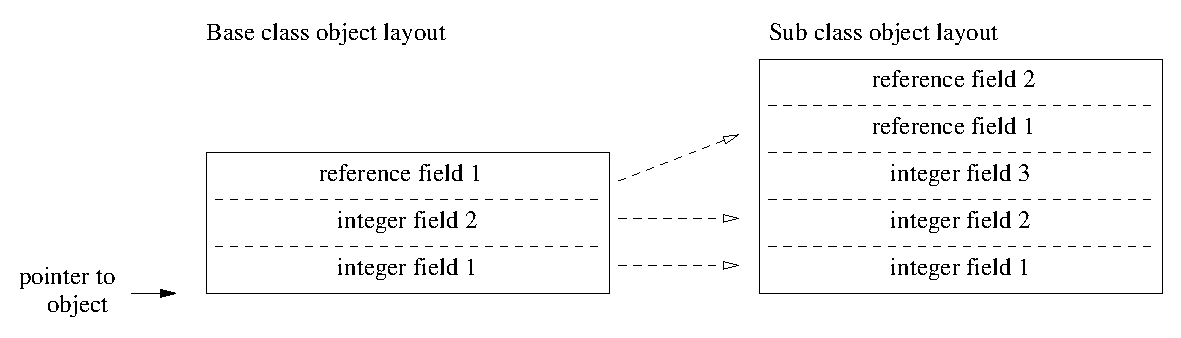
\includegraphics[width=0.7\linewidth]{super-class-sub-class-field-layout.eps}
\caption{Base class and sub class layout}
\label{fig-super-class-sub-class-field-layout}
\end{figure}

This overhead can be avoided if we can be sure of the offset at compile time, which is the case if the class is marked \mycode{final}. In this case the infuser will replace the \mycode{GETFIELD\_A} or \mycode{PUTFIELD\_A} opcode with a \mycode{\_FIXED} version so the VM knows it is safe to determine the offset at AOT compile time. Conveniently, one of the optimisations ProGuard does, is marking any class that is not subclassed as \mycode{final}, so most of this is automatic.

\paragraph{Alternative solutions} An alternative we considered is to let go of Darjeeling's split architecture for object fields and mix them, so the offsets for reference fields would also be known at compile time. To allow the garbage collector to find the reference fields we could either extend the class descriptors with a bit map indicating the type of each slot, or let the garbage collector scan all classes in the inheritance line of an object.

We chose our solution because it is easy to implement and adds only a few bytes to the VM size, while the garbage collector is already one of the most complex components of the VM. Also, we found that almost all classes in our benchmark could be marked \mycode{final}. But either solution would work, and the alternative could be considered as a more general solution.

\paragraph{Evaluation}
The impact of this optimisation is significant, but we decided not to include it in our evaluation since the overhead is the result of implementation choices in Darjeeling, which was optimised for size rather than performance. This means the overhead is a result of a Darjeeling specific choice, rather than a direct result of the AOT techniques or the JVM's design. Therefore, all results reported in this paper are with this optimisation already turned on.

Since Darjeeling's split architecture has a lot of advantages in terms of complexity and VM size, we still feel it is important to mention this as an example of the kind of trade-offs faced when optimising for performance.

\subsubsection{\mycode{SIMUL} 16-bitx16-bit to 32-bit multiplication}
While Darjeeling already introduced 16-bit arithmetic operations, it does not cover the case of multiplying two 16-bit shorts, and storing the result in a 32-bit integer. In this case the infuser would emit \mycode{S2I} instructions to convert the operands to two 32-bit integers, and then use the normal \mycode{IMUL} instruction for full 32-bit multiplication. On a device with a shorter word size, this is significantly more expensive than 16x16 to 32-bit multiplication.

We added a new opcode, \mycode{SIMUL}, for this case, which the infuser will emit if it can determine the operands are 16-bit, but the result is used as a 32-bit integer.

We could added more instructions, for example \mycode{SIADD} instruction for addition, \mycode{BSMUL} for 8-bit to 16-bit multiplication, etc. But there is always a trade-off between the added complexity of an optimisation and the performance improvement it yields, and for these cases this is much smaller than for \mycode{SIMUL}.

\subsubsection{16-bit array indexes}
Finally, normal JVM array access instructions (\mycode{IASTORE}, \mycode{IALOAD}, etc) expect the index operand to be a 32-bit integer. On a sensor node with only a few KB of memory, we will never have arrays that require such large indexes, so we modified the array access instructions to expect a 16-bit index instead. This is easily done in Darjeeling's infuser, which contains a specification of the type of operands of each opcode, and will automatically emit type conversions where necessary. In CapeVM's bytecode, the array access instructions are named \mycode{GETARRAY} and \mycode{PUTARRAY} to be in line with \mycode{GET/PUTFIELD} and \mycode{GET/PUTSTATIC}.

This complements one of the manual optimisations discussed in Section \ref{sec-optimisations-manual-java-source-optimisation}. Using short values as index variables makes operations on the index variable cheaper, while changing the operand of the array access instructions reduces the amount of work the array access instruction needs to do and the number of registers it requires.


\section{Method calls}
\label{sec-optimisations-method-calls}

Finally, we will look at the overhead caused by method calls. In native code, the smallest possible function call only has 8 cycles of overhead for a \mycode{CALL} and a \mycode{RET} instruction. More complicated functions may spend up to 76 cycles saving and restoring call-saved registers. As seen in Section \ref{sec-overhead-method-call}, in Java a considerable amount of state needs to be initialised. For the simplest method call this takes about 540 cycles, and this increases further for large methods with many parameters.

Methods in a programme typically form a spectrum from large methods at the base of the call tree that take a long time to complete and are only called a few times, to small (near-)leaf methods that are fast and frequently called. Figure \ref{fig-coremark-method-calls-vs-duration} shows this spectrum for the \mybench{CoreMark} benchmark.

For the slow methods at the base, the overhead of the method call is insignificant compared to the total execution time. However, as we get closer to the leaf methods, the number of calls increases, as does the impact on the overall performance.

At the very end of this spectrum are tiny helper functions that may be inlined, but this is only possible for very small methods, or methods called from a single place. In \mybench{CoreMark}'s case, \mycode{ee_isdigit} was small enough to inline. When larger methods are inlined, the trade-off is an increase in code size. There is a problem in the middle of the spectrum: methods that are too large to inline, but called often enough for the method call overhead to have a significant impact the overall performance.

\subsection{Lightweight methods}
For these cases we introduce a new type of method call: lightweight methods. These methods differ from normal methods in two ways:
\begin{itemize}
	\item No stack frame is created for lightweight methods, but space reserved in the caller's frame is used.
	\item Parameters are passed on the stack, rather than in local variables.
\end{itemize}

\begin{figure}
\centering
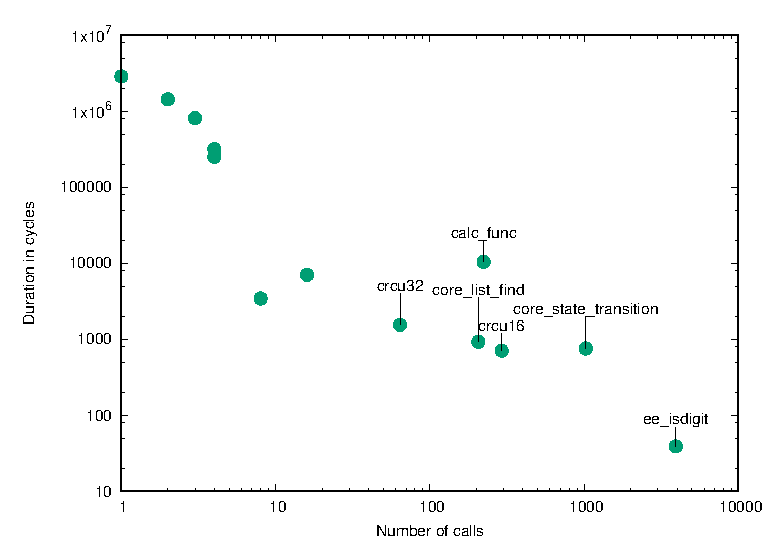
\includegraphics[width=.5\linewidth]{method-calls-vs-duration.eps}
\caption[Number of CoreMark method calls vs. duration]{Number of CoreMark method calls vs. duration (logarithmic scales)}
\label{fig-coremark-method-calls-vs-duration}
\end{figure}

Lightweight methods give us a third choice, in between a normal method call and method inlining. When calling a lightweight method, the method's AOT compiled code is called directly. This bypasses the VM completely, reusing the caller's stack frame, and leaving the parameters on the (caller's) stack. In effect, the lightweight methods behave similar to inlined code, but do not incur the code size overhead of duplicating large inlined methods. Because the method will be called from multiple locations which may have different cache states, the stack cache must be flushed to memory before a call. This results in slightly more overhead than for inlined code, but much less than for a normal method call.

As an example, consider the simple \mycode{isOdd} method in Listing \ref{lst-lightweight-stack-only}:

\begin{listing}
\centering
\begin{minipage}[t]{0.32\textwidth}
\centering
\begin{minted}{java}
// JAVA

public static boolean
          isOdd (short a)
{
  return (a & (short)1)==1;
}
\end{minted}
\end{minipage}\hfill
\begin{minipage}[t]{0.29\textwidth}
\centering
\begin{minted}{java}
// NORMAL METHOD
//              (Stack)
SLOAD_0         (Int)
SCONST_1        (Int,Int)
SAND            (Int)
SRETURN         ()
\end{minted}
\end{minipage}\hfill
\begin{minipage}[t]{0.29\textwidth}
\centering
\begin{minted}{java}
// LIGHTWEIGHT METHOD
//              (Stack)
SCONST_1        (Int,Int)
SAND            (Int)
SRETURN         ()
\end{minted}
\end{minipage}
\caption{Simple, stack-only lightweight method example}
\label{lst-lightweight-stack-only}
\end{listing}

The normal implementation has a single local variable. It expects the parameter to be stored in the local variable and the stack to be empty when we enter the method. In contrast, the lightweight method does not have any local variables and expects the parameter to be on the stack at the start of the method.

We added a new instruction, \mycode{INVOKELIGHT}, to call lightweight methods. Listing \ref{lst-comparison-lightweight-and-normal-invocation} shows how \mycode{INVOKELIGHT} and \mycode{INVOKESTATIC} are translated to native code. Both first flush the stack cache to memory. After that, the lightweight invocation can directly call the implementation of \mycode{isOdd}, while the normal version first saves the stack pointers, and then enters an expensive call to the \mycode{callMethod} function in the VM, which will set up a stack frame for \mycode{isOdd}, and then call the actual method.

\begin{listing}
\centering
\begin{minipage}[t]{0.5\textwidth}
\centering
\begin{minted}{java}
// NORMAL INVOCATION
// INVOKESTATIC isOdd:
    push r25        // Flush the cache
    push r24
    call &preinvoke // Save X and SP
    ldi r22, 253    // Set parameters
    ldi r23, 2      //  for callMethod
    ldi r24, 21
    ldi r20, 64
    ldi r21, 42
    ldi r18, 13
    ldi r19, 0
    ldi r25, 2
    call &callMethod // Call to VM
    call &postinvoke // Restore X and SP
\end{minted}
\end{minipage}\hfill
\begin{minipage}[t]{0.45\textwidth}
\centering
\begin{minted}[linenos=false]{java}
// LIGHTWEIGHT INVOCATION
// INVOKELIGHT isOdd:
    push r25      // Flush the cache
    push r24
    call &isOdd
\end{minted}
\end{minipage}
\caption{Comparison of lightweight and normal method invocation}
\label{lst-comparison-lightweight-and-normal-invocation}
\end{listing}

\subsubsection{Local variables}
The lightweight implementation of the \mycode{isOdd} example only needs to process the values that are on the stack, but this is only possible for the smallest methods. If a lightweight method has local variables, space is reserved for them in the caller's stack frame, equal to the maximum number of slots needed by all the lightweight methods it may call.

CapeVM uses the ATmega's Y register to point to the start of a method's local variables. To call a lightweight method with local variables, the caller only needs to shift Y up to the region reserved for lightweight method variables before doing the \mycode{CALL}. The lightweight method can then access its locals as if it were a normal method. After the lightweight method returns, the caller lowers Y, so it points to the caller's own variables again.

\subsubsection{Nested calls}
A final extension is to allow for nested calls. While frequently called leaf methods benefit the most from lightweight methods, there are many cases where it is useful for one lightweight methods to call another. A good example from the \mybench{CoreMark} benchmark is the 32-bit \mycode{crcu32} function, which is implemented as two calls to \mycode{crcu16}. For the best performance, both methods should be lightweight.

So far we have not discussed how to handle the return address in a lightweight method. The AOT compiler uses the native stack to store VM's integer stack value, which means the operands to a lightweight method will be on the native stack. But after a native \mycode{CALL} instruction, the return address is also put on the native stack, covering the method parameters.

For leaf methods, the lightweight method will first pop the return address into two fixed registers, and avoid using these register for stack caching. When the method returns, the return address is pushed back onto the stack just before the \mycode{RET} instruction.

For lightweight methods that will call another lightweight method, the return value is also popped from the stack, but instead of leaving it in the fixed register, where it would be overwritten by the nested call, it is saved in the first local variable slot and Y is incremented to skip this slot. Since each lightweight method has its own block of locals, lightweight calls can be nested as deeply as needed.

This difference in method prologue and epilogue is the only difference in the way the VM generates code for a lightweight method, all bytecode instructions can then be translated the same way as for a normal method.

\subsubsection{Stack frame layout}
A normal method that invokes a possible string of lightweight methods, needs to save space for this in its stack frame. How much space it needs to reserve can be determined by the infuser at compile time, and this information is added to the method header used to create the stack frame.

% For each method the number of locals is known by the infuser. If it is a lightweight method that will call another lightweight, one extra slot is reserved for the return address. In addition, each method needs to reserve the maximum number of extra slots required for of any lightweight method it may call. Since we can only call one at a time, they can all use the same space reserved in the caller's stack frame. A similar calculation is done to determine any extra reference stack space needed to accommodate the lightweight methods that may be called.

\begin{figure}
\centering
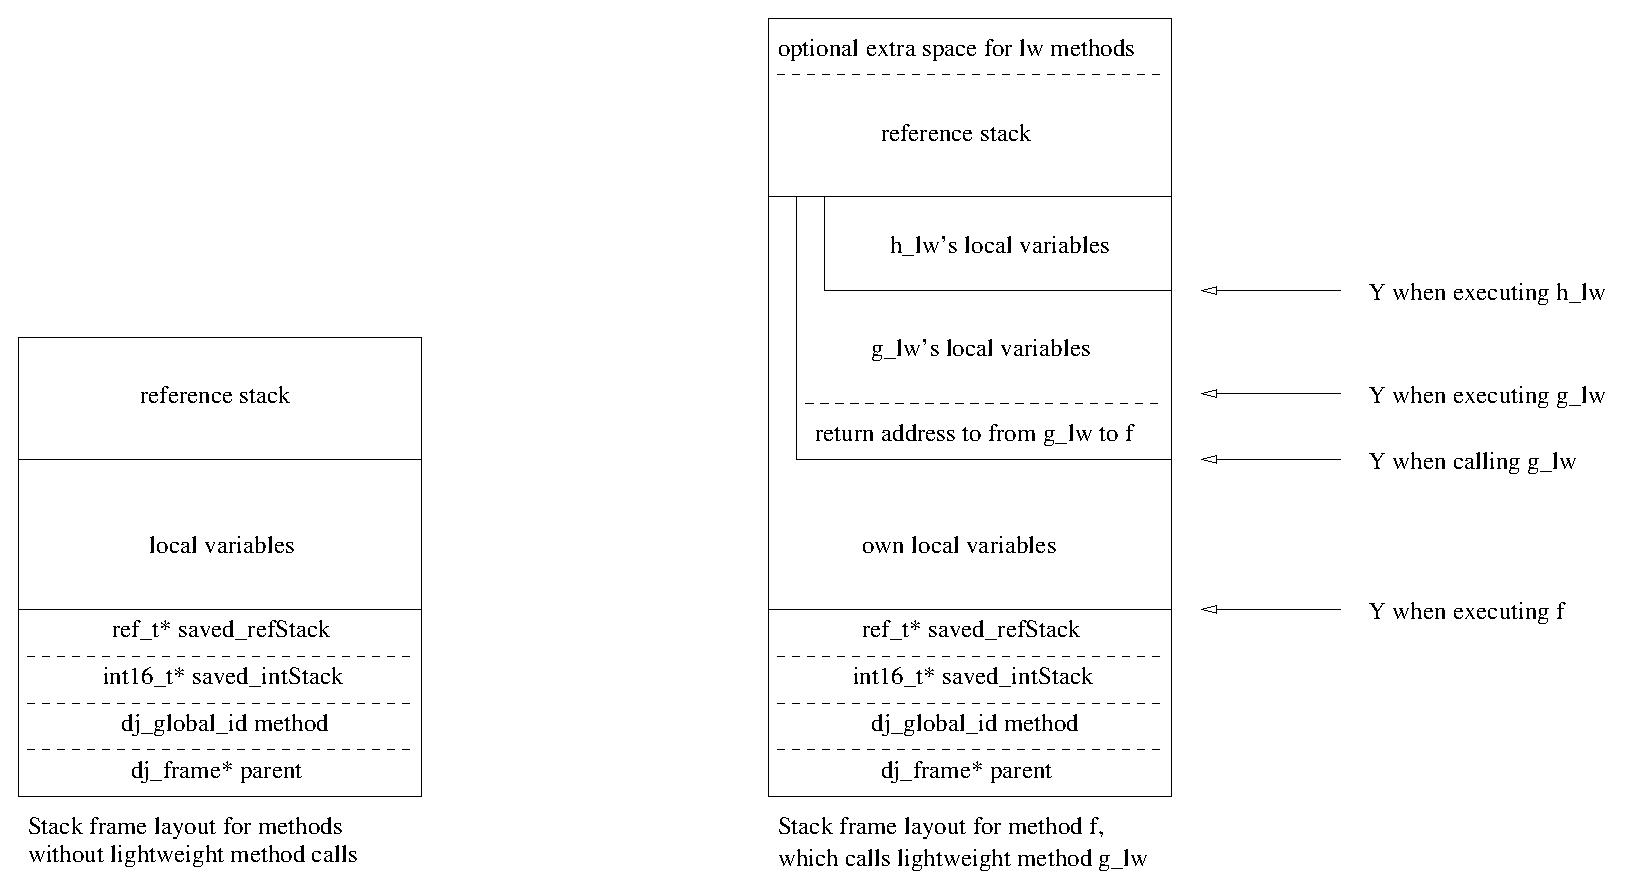
\includegraphics[width=0.95\linewidth]{stack-frame-lightweight-method.eps}
\caption{Stack frame layout for a normal method \mycode{f}, which calls lightweight method \mycode{g_lw}, which in turn calls lightweight method \mycode{h_lw}}
\label{fig-stack-frame-lightweight-method}
\end{figure}

An example is shown in Figure \ref{fig-stack-frame-lightweight-method}, which shows the stack frame for a normal method \mycode{f}, which calls lightweight method \mycode{g_lw}, which in turn calls another lightweight method \mycode{h_lw}.

The stack frame for \mycode{f} contains space for its own locals, and for the locals of the lightweight method it calls: \mycode{g_lw}. In turn, \mycode{g_lw}'s locals contain space for \mycode{h_lw}'s locals, as well as a slot to store the return address back to \mycode{f}. Since \mycode{h_lw} does not call any other methods, it just keeps its return address in registers.

When a method calls a lightweight method with local variables, it will move the Y register to point to that method's locals. From Figure \ref{fig-stack-frame-lightweight-method} it is clear it only needs to increment Y by the size of its own locals. For \mycode{f}, this will place the Y register at the beginning of \mycode{g_lw}'s locals. Since \mycode{g_lw} may call \mycode{h_lw}, \mycode{g_lw}'s prologue will first store the return address in the first local slot, moving Y forward in the process so that Y points to the first free slot.

\subsubsection{Mark loops}
Lightweight methods may use any register and do not save call-saved registers like normal methods. When a lightweight method is called inside a \mycode{MARKLOOP} block, it may corrupt some of the variables pinned to registers. In this case the caller saves those variables back to memory before calling the lightweight method and loads them again after the call returns. Since lightweight methods always come before their invocation in the infusion, the VM already knows which registers it uses, and will only save and restore pinned variables if there is a conflict. Because registers for \mycode{MARKLOOP} are allocated low to high, and for normal stack caching from high to low, in many cases the two may not collide.

\subsubsection{Example call}
An example of the most complex case for a lightweight call is shown in Listing \ref{lst-full-lighweight-method-call}, which shows how method \mycode{f} from Figure \ref{fig-stack-frame-lightweight-method} would call \mycode{g_lw}, assuming \mycode{f} is in a \mycode{MARKLOOP} block at the time which pinned a variable R14:R15, and these registers are also used by \mycode{g_lw}.

In the translation of the \mycode{INVOKELIGHT} instruction, first the stack cache is flushed to memory, then the value of the local variable at offset 22 is saved because it was pinned to R14:R15. Next, the Y register is incremented to skip the caller's own local variables and point Y to the start of the space reserved for lightweight method locals.

In the implementation of \mycode{g_lw}, the return address is popped off the stack into R18:R19. Since \mycode{g_lw} may call another lightweight method which will do the same, the return address is stored in the first local slot, incrementing Y in the process. After \mycode{g_lw}'s body, the return address is pushed back onto the stack before the final \mycode{ret} instruction.

After \mycode{g_lw} returns, the reverse process is used to return to the caller: the Y register is restored to point to the caller's locals, and the local variable at offset 22 is loaded back into the pinned registers R14:R15.

\begin{listing}
\centering
\begin{minipage}[t]{0.48\textwidth}
\begin{minted}{java}
// LIGHTWEIGHT INVOCATION
INVOKELIGHT g_lw
    push r25        // Flush the cache
    push r24
    std Y+22, r14   // Save pinned value
    std Y+23, r15
    adiw Y, 26      // Move Y to g_lw's
    call &g_lw                 // locals












    sbiw Y, 26      // Restore Y
    ldd r14, Y+22   // Reload pinned value
    ldd r15, Y+23
\end{minted}
\end{minipage}\hfill
\begin{minipage}[t]{0.48\textwidth}
\centering
\begin{minted}[linenos=false]{java}
// IMPLEMENTATION OF g_lw







    pop r18     // Pop the return address
    pop r19
    st Y+, r18  // Save in 1st local slot,
    st Y+, r19  //  and increment Y

      .. // g_lw's body

    ld r19, -Y  // Load return address,
    ld r18, -Y  //  and decrement Y
    push r19    // Push return address
    push r18    //  onto the stack
    ret



\end{minted}
\end{minipage}
\caption{Full lightweight method call}
\label{lst-full-lighweight-method-call}
\end{listing}


\subsection{Creating lightweight methods}
CapeVM currently supports two ways to create lightweight methods:
\begin{itemize}
	\item Handwritten bytecode
	\item Converted Java methods
\end{itemize}

\subsubsection{Handwritten bytecode}
For the first option, a method is declared \mycode{native} in the Java source code, so the code calling it will compile as usual. The infuser is provided with a handwritten implementation in bytecode, which it will simply add to the infusion, and then process in the same way it processes a normal method, with one additional step:

For lightweight methods, the parameters will be on the stack at the start of the method, but the infuser expects to start with an empty stack. To allow the infuser to process them like other methods, a dummy \mycode{LW_PARAMETER} instruction is added for each parameter. This instruction is skipped when writing the binary infusion, but it tricks the infuser into thinking the parameters are being put on the stack.

\subsubsection{Converted Java methods}
This handwritten approach is useful for the smallest methods, and allows us to create bytecode that only uses the stack, which produces the most efficient code. But for more complex methods it quickly becomes very cumbersome to write the bytecode by hand.

As a second, slightly slower, but more convenient option, normal Java methods can be converted to lightweight methods by adding a \mycode{@Lightweight} annotation to it.

The infuser will scan all the methods in an infusion for this annotation. When it finds a method marked \mycode{@Lightweight}, the transformation to turn a normal method into a lightweight one is simple: for each parameter, a dummy \mycode{LW_PARAMETER} instruction is added to the start of the method, followed by a \mycode{STORE} instruction to pop the parameter off the stack and store it in the right local variable. After this, the method can be called as a lightweight method.

Listing \ref{lst-comparison-of-handwritten-and-converted-java-lw-method} shows the difference for the \mycode{isOdd} method. We can see this approach adds some overhead in the form of a \mycode{SSTORE_0} and a \mycode{SLOAD_0} instruction. However, using popped value caching, only the \mycode{SSTORE_0} will have a run-time cost. Another disadvantage of the converted method is that it uses a local variable, which will slightly increase memory usage, but in return this approach gives us a very easy way to create lightweight methods.

\begin{listing}
 \centering
 \begin{minipage}[t]{0.32\textwidth}
  \centering
  \begin{minted}{java}
// JAVA
@Lightweight
public static boolean
          isOdd (short a)
{
  return (a & (short)1)==1;
}
  \end{minted}
 \end{minipage}\hfill
 \begin{minipage}[t]{0.29\textwidth}
  \centering
  \begin{minted}[linenos=false]{java}
// HANDWRITTEN
//              (Stack)
LW_PARAMETER    (Int)
SCONST_1        (Int,Int)
SAND            (Int)
SRETURN         ()
  \end{minted}
 \end{minipage}\hfill
 \begin{minipage}[t]{0.29\textwidth}
  \centering
  \begin{minted}[linenos=false]{java}
// CONVERTED JAVA
//              (Stack)
LW_PARAMETER    (Int)
SSTORE_0        ()
SLOAD_0         (Int)
SCONST_1        (Int,Int)
SAND            (Int)
SRETURN         ()
  \end{minted}
 \end{minipage}
 \vspace{0.5cm}

\caption{Comparison of hand written lightweight method and converted Java method}
\label{lst-comparison-of-handwritten-and-converted-java-lw-method}
\end{listing}

\subsubsection{Replacing \mycode{INVOKE}s}
The infuser does a few more transformations to the bytecode. Every method is scanned for \mycode{INVOKESTATIC} instructions that invoke a lightweight method. These are simply replaced by an \mycode{INVOKELIGHT} instruction, and the number of extra slots for the reference stack and local variables of the current method is increased if necessary. Finally, methods are sorted so a lightweight method will be defined before it is invoked, to ensure the VM can always generate the \mycode{CALL} directly.

\subsection{Overhead comparison}
We now compare the overhead for the various ways we can call a method in Table \ref{tbl-method-invoke-overhead-comparison}.

Manually inlining code yields the best performance, but at the cost of increasing code size if larger methods are inlined. ProGuard inlining is slightly more expensive because it always saves parameters in local variables.

Both lightweight methods options cause some overhead, although this is very little compared to a full method call. First, we need to flush the stack cache to memory to make sure the parameters are on the real stack. This this takes two \mycode{push} and eventually two corresponding \mycode{pop} instructions per word, costing 8 cycles per word. In addition, we need to clear the value tags from the stack cache, which means we may not be able to skip as many \mycode{LOAD} instructions after the lightweight call, but the effect of this is hard to quantify.

Next the cost of translating the \mycode{INVOKE} instruction varies depending on the situation. In the simplest case it is simply a \mycode{CALL} to the lightweight method, which together with the corresponding \mycode{RET} costs 8 cycles. The worst case is 68 cycles when the lightweight method has local variables, uses all registers, and the caller used the maximum of 7 pairs to pin variables in a \mycode{MARKLOOP} block.
%INVOKE COST FOR LIGHTWEIGHT METHOD:
%  8            CALL/RET
%  4            move Y
%  8 per word   saving markloop pinned registers used by lw method
%  0            pre/post invoke
%  0            setup callMethod parameters
%  
%  minimum: 8
%  maximum: 8 + 4 + 8*7 = 68
%  
%INVOKE COST FOR NORMAL METHOD:
%  8            CALL/RET
%  0            move Y
%  0            saving markloop pinned registers used by lw method
%  32+34        pre/post invoke
%  8            setup callMethod parameters
%  
%  total: 8+ = 82
\begin{table}
\caption{Approximate cycles of overhead caused by different ways of invoking a method}
\label{tbl-method-invoke-overhead-comparison}
	\centerline{
    \begin{tabular}{lccccc} % NO SIMULATION DATA
    \toprule
                                                              & Manual          & ProGuard                & Stack-only                  & Converted Java              & Normal                                              \\
                                                              & inlining        & inlining                & lightweight                 & lightweight                 & method call                                         \\
    \midrule
    \midrule
    flush the stack cache
                                                              &                 &                         & 8 per word                  & 8 per word                  & 8 per word                                          \\
    \mintinline[fontsize=\footnotesize]{java}{INVOKE}                                           &                 &                         & 8 to 68                     & 8 to 68                     & \textasciitilde 80                                  \\
% was (20180303)    \mycode{INVOKE}                                           &                 &                         & 8 to 68                     & 8 to 68                     & \textasciitilde 82                                  \\
    create stack frame                                        &                 &                         &                             &                             & \textasciitilde 450                                 \\
    method pro-/epilogue                                      &                 &                         & 8 or 16                     & 8 or 16                     & 10 to 71                                            \\
    store and load parameters                                 &                 & 4 or 8 per word         &                             & 4 or 8 per word             & 4 or 8 per word                                     \\
    \\
% was (20180303)    \emph{total}                                              &                 & \emph{4 or 8 per word}  & \emph{16 to 84 +}           & \emph{16 to 84 +}           & \emph{\textasciitilde 542 to \textasciitilde 603 +} \\
    \emph{total}                                              &                 & \emph{4 or 8 per word}  & \emph{16 to 84 +}           & \emph{16 to 84 +}           & \emph{\textasciitilde 540 to \textasciitilde 601 +} \\
                                                              &                 &                         & \emph{8 per word}           & \emph{12 or 16 per word}    & \emph{12 or 16 per word}                            \\
    \bottomrule
    \end{tabular}
    }
\end{table}


After calling the method, the method prologue for lightweight methods is very simple. It saves the return address and restores it in the epilogue, which takes 8 cycles if left in a register, or 16 if it needs to be stored in a local variable slot.

For small handwritten lightweight methods this is the only cost, but for larger ones created by converting a Java method, we add \mycode{STORE} instructions to copy the parameters from the stack into local variables, as shown in Listing \ref{lst-comparison-of-handwritten-and-converted-java-lw-method}. This is similar to the only overhead incurred by ProGuard's method inlining, and costs 4 cycles per word for the \mycode{STORE}, and possibly 4 more if the corresponding \mycode{LOAD} cannot be eliminated by popped value caching.

The total overhead for a lightweight method call scales nicely with the method's complexity. For the smallest methods, the minimum is only 16 cycles, plus 8 cycles per word for the parameters. For the most complex cases this may go up to 100 to 150 cycles. But these methods must be more complex and will have a longer run time, which limits the relative overhead.

The number of cycles in Table \ref{tbl-method-invoke-overhead-comparison} is just a broad indication of the overhead. Some factors, such as the cost of clearing the value tags is hard to predict, and inlining may allow optimisations that are not possible with a method call. In practice the actual cost in a number of specific cases we examined varies, but is in the range we predicted.

For a normal method call the cost is much higher, and less dependent on the complexity of the method that is called. The overhead from setting up the stack frame, and the more expensive translation of the \mycode{INVOKE} instruction (see Listing \ref{lst-lightweight-stack-only}) are fixed, meaning a call will cost at least around 540 cycles, increasing to over 700 cycles for more complex methods taking many parameters.




\subsection{Limitations and trade-offs}
There are a few limitations to the use of lightweight methods:

\paragraph{No recursion} Since the infuser needs to be able to determine how much space to reserve in the caller's stack frame for a lightweight method's reference stack and local variables, recursion is not supported, although lightweight calls can be nested. While this is clearly a limitation, recursive code is not common on sensor nodes because of the limited amount of memory available.

\paragraph{No garbage collection}
Lightweight methods reuse the caller's stack frame. This is a problem for the garbage collector, which works by inspecting each stack frame and finding the references on the stack and in local variables. If the garbage collector would be triggered while a lightweight method is being executed, it would not know where to find the lightweight method's references, since the stack frame only has information for the method that owns it. Thus, lightweight methods cannot perform any action that may trigger the garbage collector.

While it may be possible to relax this constraint with some effort, in most cases this is only a minor restriction. Lightweight methods are most useful for fast and frequently called methods, and operations that may trigger the garbage collector are usually expensive, so there is less to be gained from using a lightweight method in these situations.

\paragraph{Static only}
Lightweight virtual methods are not supported, but this is something that could be considered in future work. However, in all our benchmarks, virtual methods were only used in a single case that could easily be transformed into code using static methods (see Section \ref{sec-evaluation-coremark-non-automatic-optimisations}).

\paragraph{Stack frame memory usage}
Finally, we should remember that a method calling a lightweight method always reserves space for it in its locals. This space is reserved, regardless of whether the lightweight method is currently executing or not, and the more nested lightweight calls are made, the more space needs to be reserved.

As an example, consider a method \mycode{f1} which may call a lightweight method with a large number of local variables, \mycode{big_lw}, but is currently calling normal method \mycode{f2}, which may also call \mycode{big_lw}. In this case space for \mycode{big_lw} will be reserved twice, both in \mycode{f1}'s and in \mycode{f2}'s frame. Thus, some restraint should be used when making larger methods at the top of the call tree lightweight.


\chapter{Safety}
\label{sec-safety}
\newcounter{tcheckcnt}
\newcommand{\tcheck}[1]{\refstepcounter{tcheckcnt}T-\arabic{tcheckcnt}\label{#1}}
\newcounter{rcheckcnt}
\newcommand{\rcheck}[1]{\refstepcounter{rcheckcnt}R-\arabic{rcheckcnt}\label{#1}}

\makeatletter
\renewcommand\p@tcheckcnt{T-\arabic{tcheckcnt}\expandafter\@gobble}
\renewcommand\p@rcheckcnt{R-\arabic{rcheckcnt}\expandafter\@gobble}
\makeatother

\begin{table}
\caption{List of safety checks}
\label{tbl-safety-checks}
    \begin{tabular}{lp{0.9\linewidth}} % NO SIMULATION DATA
    \toprule
     & Translation-time checks \\

    \tcheck{chk-method-header-is-sane}
        & For each method header, the number of own local variable slots <= the number of total variable slots, the number of (int/ref) arguments <= the number of (int/ref) variables, static methods are not abstract. \\

    \tcheck{chk-return-or-goto-at-end-of-method}
        & The last instruction of each method is a \mycodetbl{RETURN} or \mycodetbl{GOTO}. \\

    \tcheck{chk-brtarget-exists}
        & Branch instructions branch to an index < the number of \mycodetbl{BRTARGET}s announced in the method header. \\

    \tcheck{chk-all-brtargets-found}
        & At the end of each method, we have seen the exact number of \mycodetbl{BRTARGET} instructions announced in the method header. \\

    \tcheck{chk-invokelight-target-found}
        & The target for an \mycodetbl{INVOKELIGHT} call is already translated, so the target address is known. \\

    \tcheck{chk-invokestatic-target-header-found}
        & The target method header for an \mycodetbl{INVOKESTATIC}/\mycodetbl{INVOKESPECIAL} exists. \\

    \tcheck{chk-stack-is-empty-after-return}
        & After popping the return value, the stack is empty. \\

    \tcheck{chk-sufficient-stack-space-at-invokelight}
        & At the point of an \mycodetbl{INVOKELIGHT} instruction, the max stack of the caller >= the current stack depth - the number of arguments to the callee + the max stack of the callee, for both integer and reference stacks. \\

    \tcheck{chk-no-operandstack-underflow}
        & Before each instruction, the stack depth >= the number of elements to be consumed by the instruction. \\

    \tcheck{chk-no-operandstack-overflow}
        & After each instruction, the stack depth <= the max stack depth announced in the header. \\

    \tcheck{chk-stack-is-empty-at-branches}
        & The stack is empty at branches and branch targets. \\

    \tcheck{chk-sufficient-locals-at-invokelight}
        & For each \mycodetbl{INVOKELIGHT}, the total number of slots - the number of own variable slots for the caller >= the total variable slots for the callee. \\

    \tcheck{chk-local-variable-slot-exists}
        & The index of the local variable < the number of own variable slots for the current method. \\

    \tcheck{chk-static-variable-infusion-exists}
        & The target infusion of a static variable exists. \\

    \tcheck{chk-static-variable-slot-exists}
        & The index of the static variable < the number of static variable slots for the target infusion. \\

    \midrule
    & Run-time checks \\

    \rcheck{chk-invokevirtual-target-found}
        & The target implementation for an \mycodetbl{INVOKEVIRTUAL}/\mycodetbl{INVOKEINTERFACE} is found. \\

    \rcheck{chk-no-nativestack-overflow}
        & Whenever a new stack frame is allocated the frame+max stack depth+some safety margin > the end of the heap. \\

    \rcheck{chk-invokevirtual-stack-effects-match}
        & The target implementation for an \mycodetbl{INVOKEVIRTUAL}/\mycodetbl{INVOKEINTERFACE} matches the stack effects used to verify the caller's stack at translation time. \\

    \rcheck{chk-memory-access-within-heap}
        & The target address of an array element or object field is within the heap. \\

    \rcheck{chk-gc-heap-integrity}
        & The headers of heap chunks form a consistent chain of chunks, ending at the byte indicated by a pointer to the first free heap byte. \\

    \bottomrule
    \end{tabular}
\end{table}

The second goal of this dissertation is to develop a VM that offers a 'safe' execution environment, and to compare the cost of doing so using a VM, to existing native code approaches.

A safe execution environment is one that guarantees an application cannot harm the system it is running on or other applications running on the same system. Specifically, an application cannot:
\begin{enumerate}
    \item Execute code it does not have permission for,
    \item Write to memory outside the areas assigned to it, or
    \item Retain control of the CPU indefinitely
\end{enumerate}

Given the first two, the last guarantee is easy to implement: the VM can simply set a timer to trap back to the VM after a certain amount of time. As long as the other guarantees hold, the application will not be able to disable the timer without the VM's permission. To guard against programming errors as well as malicious attacks, we focus on the second type of approaches shown in Figure \ref{fig-safe-compilation-process}, where the node does not rely on a trusted host to guarantee safety, but can do so independent of the code it receives.

As discussed in Chapter 3, most generic sensor nodes VMs do not consider safety, with the exception of SensorScheme \cite{Evers:2010ur}, although a number of native code systems have been proposed. This is unfortunate because using a VM has some distinct advantages compared to native code systems that guarantee safety.

Both the machine model and the instruction set of the virtual machine are more structured than a real CPU. This restricts what a bytecode instruction can do, which in turn allows the VM to verify safety for many instructions at translation time.

As an example, memory on the physical CPU is a flat address space, and the ATmega's store instructions can write to \emph{any} address in memory. In the VM, memory for local variables, static variables, and for objects and arrays, are separated and the VM has separate instructions to target each of them as an offset within their respective regions. Similarly, native code can branch to any address within flash memory, while the VM's branches target the id of a branch target within the current method.

While in CapeVM, the programme eventually also runs as native code on the physical CPU, the VM is in complete control of how this code is generated and the context in which it runs. As shown in the next sections, this make it easy to determine at translation time that stores to local and static variables will write to space reserved for a local or static variable, and that branches will branch to a legal instruction within the method.

Table \ref{tbl-safety-checks} contains the list of checks done by CapeVM to guarantee safety. To show these are sufficient to satisfy the high level guarantees listed before, we first express them as concrete constraints specific to CapeVM:

\begin{itemize}
    \item \emph{control flow safety}: after starting the application, the VM is always executing either
        \begin{itemize}
            \item a translated bytecode instruction in the current method \emph{from the start}, or
            \item code in the VM itself, as a result of either a call to a VM function from a translated bytecode instruction, or returning from a method
        \end{itemize}
    \item \emph{memory safety}: any write to memory done by the application is to a legal location: either
        \begin{itemize}
            \item memory reserved for the operand stack, or
            \item a valid local or static variable slot, or
            \item the area of the heap assigned to the application
        \end{itemize}
\end{itemize}

The control flow guarantees make sure code cannot jump to a point half-way a generated instruction to skip run-time checks, or to anywhere in the VM except through the proper entry points defined by the VM. As in normal Java, the bytecode instructions in CapeVM can only modify state within the virtual machine. There are no special instructions to access sensors and actuators as in for example Maté. Thus, access to external resources is assumed to happen through calls to natively implemented library functions, which returns control to VM and allows it to check whether the application has permission to do so.

Clearly, the VM will be in a legal state when a programme starts: the VM will jump to the begining of the first instruction and no writes will have occured yet. We will show the checks in Table \ref{tbl-safety-checks} are sufficient to ensure these two constraints, by examining how each bytecode instruction can affect control flow and write to memory, and list the checks necessary to ensure the VM is still in a legal state after executing it. Both guarantees depend on each other: memory safety is assumed when discussing control flow safety and vice versa.

Each method in CapeVM has a small \emph{method header} defining properties such as the maximum stack size, number of local variables, return type, etc. The VM uses this header to create the stack frame, and to determine the effects of call to that method on the caller's operand stack, Therefore, many of the checks are to ensure the implementation of the method follows the contract established in the method header. When the node receives new code, it first receives the headers for all methods, followed by their implementations, so the contracts for all methods are known when the bytecode is translated.

The first check is a basic sanity check on the data in the method headers (\ref{chk-method-header-is-sane}). Since each parameter becomes a local variable, the number of local variable slots must be at least as high as the number of parameters, and the total number of slots must be at least as high as the method's own local variable slots, while the rest may be used for lightweight methods. Finally, a method cannot be marked static and abstract at the same time.

\section{Control flow safety}
We show control flow safety by considering the effect of all bytecode instructions, and showing they either flow into the start of a legal next instruction, or return control back to the VM. Regarding their effect on control flow, the bytecode instructions can be grouped into four categories, shown in Table \ref{tbl-control-flow-instructions}. The state is correct at the start of the programme, since the VM will start it by jumping to the beginning of the first instruction in the main method. We will show the state will be correct after each following instruction by looking at these four categories.

\begin{table}
\caption{Instructions affecting control flow}
\label{tbl-control-flow-instructions}
    \begin{tabular}{ll} % NO SIMULATION DATA
    \toprule
    Type              & Effect on control flow \\
    \midrule
    \midrule
    Branches          & Jump to a location within the method \\
    \mycode{INVOKE}s  & Call a method, either through the VM or directly \\
    \mycode{RETURN}s  & Return to the address at the top of the stack \\
    Others            & Fall through to the next bytecode instruction \\
    \bottomrule
    \end{tabular}
\end{table}

\subsection{Simple instructions}
Starting with the last category: most instructions such as math operations, loads and stores, are translated to a sequence of native instructions that will be executed top to bottom. In some cases this may call to a VM or \mycode{libc} function to perform some complex operation, temporarily handing control back to the VM, but these calls return to the current instruction once the operation is complete.

For this category, the generated code will flow naturally into the start of the next generated instruction. This is means the control flow constraint would be broken if there is no next instruction, which produces the second translation-time check, \ref{chk-return-or-goto-at-end-of-method}: the last instruction in a method must be a \mycode{RETURN} or \mycode{GOTO} to prevent control from flowing out of the method body.

\subsection{Branch instructions}
In CapeVM bytecode, branches do not target an offset as in normal JVM bytecode, but the id of a branch target. These targets are marked with a \mycode{BRTARGET} instruction, which does not emit any code, but causes the AOT compiler to collect the address in a temporary table during translation. Once the whole method is translated, this temporary table is used to patch the correct target address into the branch instructions.

Each method announces the number of branch targets that will be used in the method header. Non-taken branches flow into a correct next instruction because \ref{chk-return-or-goto-at-end-of-method} guarantees they are not the last instruction in a method. To ensure a taken branch will branch to the start of an instruction within the method, two checks are needed: the target ID of each branch must be lower than number of branch targets announced in the method header (\ref{chk-brtarget-exists}), and at the end of the method the number of \mycode{BRTARGET} instructions encountered must be equal to the number announced in the header (\ref{chk-all-brtargets-found}). The first guarantees each branch refers to an entry in the temporary table, while the second guarantees all entries are filled with a valid address.

\subsection{Method invocation instructions}
There are three kinds of method invocations.

For lightweight method calls, the implementation of the target method is required to come before any method invoking it, to ensure the address of the target is known at translation time and we can directly generate a \mycode{CALL} to the method. Ensuring this calls to a correct address is therefore trivial: for \mycode{INVOKELIGHT} instructions, the implementation of the target method must already have been generated (\ref{chk-invokelight-target-found}).

For static calls (\mycode{INVOKESTATIC} and \mycode{INVOKESPECIAL}) the target method is known at translation time, but it may not have been translated yet if the implementation follows later in the infusion. For these instructions, a \mycode{CALL} to the VM's \mycode{callMethod} function is generated, passing the id of the target method as a parameter. At run time this id will be used as an index in the method table to find its implementation. Because the VM receives all the method headers before translating their implementations, it can check at translation time that the method id is known (\ref{chk-invokestatic-target-header-found}). Since the VM will not start an application before all methods are translated, this guarantees that \mycode{callMethod} will find the target at run time.

Finally, for \mycode{INVOKEVIRTUAL} and \mycode{INVOKEINTERFACE}, the target is not known at translation time, since this depends on the object the method is invoked on. Darjeeling does not use dispatch tables to call virtual methods. Instead, each infusion contains a flattened list of methods that are scanned to find the right implementation for the current object. Therefore a run-time check is needed to verify the method can be found (\ref{chk-invokevirtual-target-found}), but since this is necessary to make the call, this check does not add any extra overhead.

Again, once the call returns, check \ref{chk-return-or-goto-at-end-of-method} ensures control will flow into a valid next instruction.

\subsection{Return instructions}
\label{sec-control-flow-safety-return-instructions}
Finally, return instructions pop the return value from the stack, and then do a native \mycode{RET} instruction to exit the method and return control, either directly to the AOT compiled code of the caller for lightweight method calls, or to the VM's \mycode{callMethod} function for normal methods.

The \mycode{RET} instruction takes the return address from the native stack, which is also used to store the VM's integer operand stack. This means the integer operand stack needs to be empty at return instructions (\ref{chk-stack-is-empty-after-return}) to ensure the correct address will be at the top of the native stack. Memory safety then guarantees the application could not have corrupted it. Without this check, malicious code could leave an integer on the stack and use the return instruction to jump to an arbitrary location.

A second way the return address could be corrupted is if the native stack overflows into the VM's heap. In CapeVM the heap is a fixed sized block that sits above other global variables, and below the native stack that grows down towards it. If the native stack grows into the area reserved for the heap, a return address may be corrupted by an otherwise valid heap write.

To prevent this, a run-time check is added to non-lightweight invokes, that checks the stack frame for the called method, plus its maximum integer stack size, does not grow into the heap (\ref{chk-no-nativestack-overflow}). Lightweight calls do not add to the stack, since space for their local variables, stack, and return address was already allocated in the caller's frame.

While running, a method may make calls to the VM or \mycode{libc} functions, causing the stack to grow further. Since the maximum stack growth for such calls is fixed, a certain safety margin is added between the stack and heap. A similar gap of 128 bytes between the stack and kernel heap is reserved by \emph{t-kernel} \cite{Gu:2005un}, although it is not clear from the paper whether this is for the same reason.




\section{Memory safety}

\begin{figure}
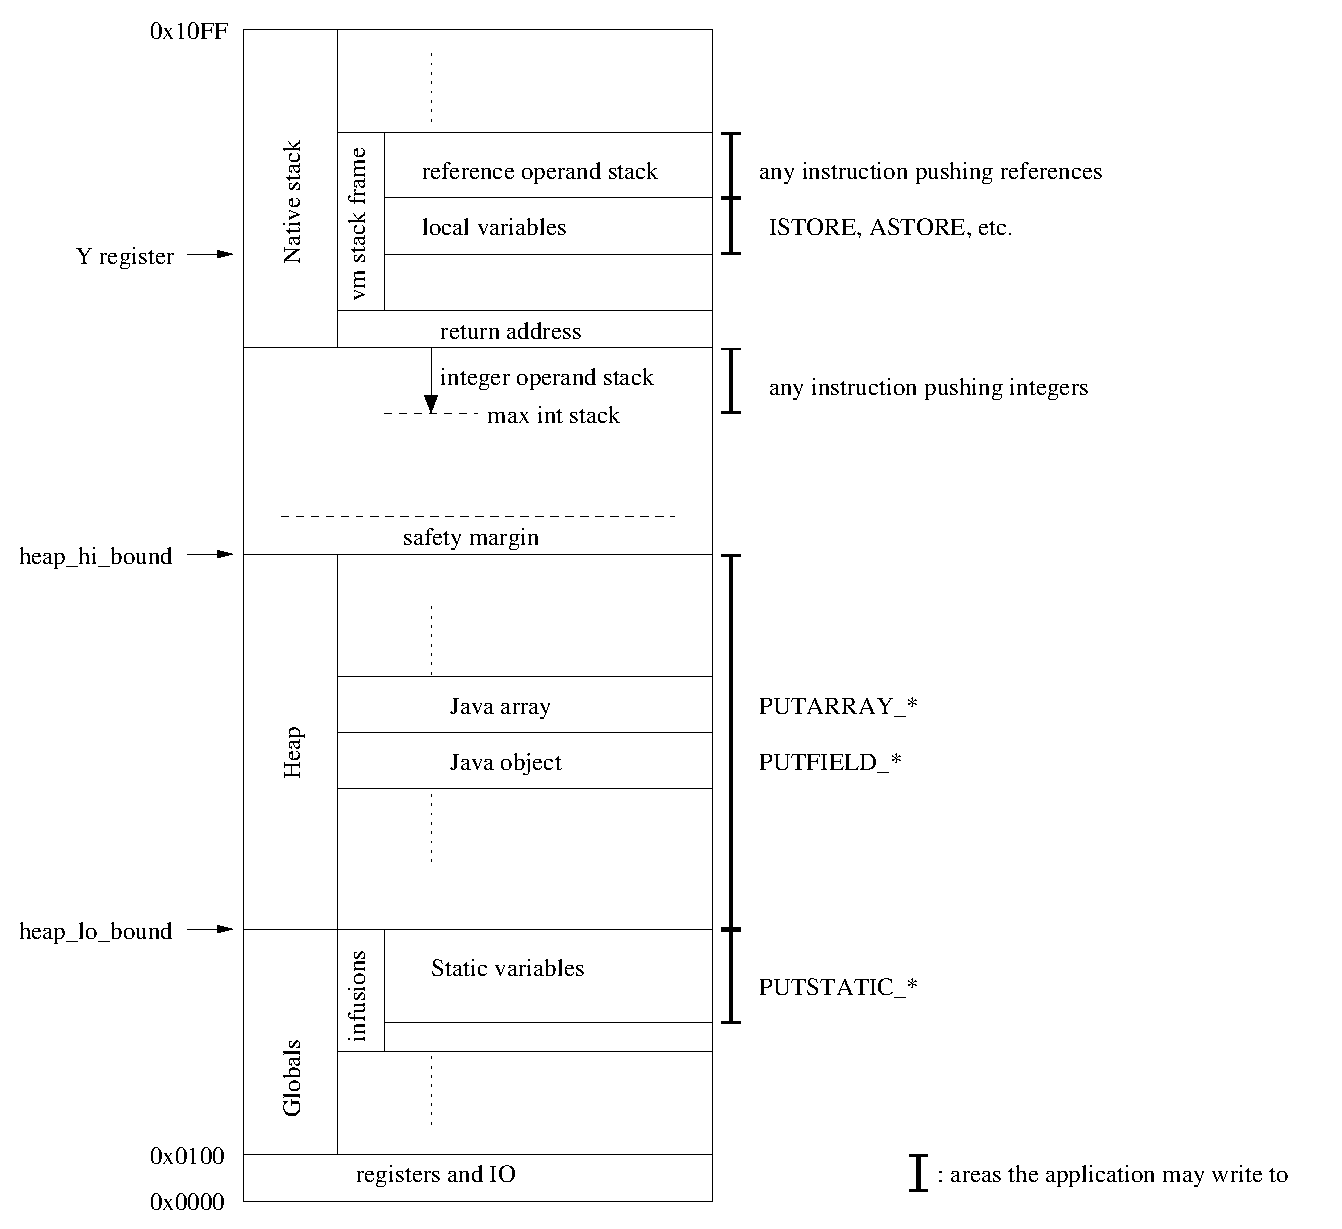
\includegraphics[width=\linewidth]{memlayout.eps}
\caption{Global memory layout and the areas accessible to the application}
\label{fig-memlayout}
\end{figure}

Figure \ref{fig-memlayout} shows the global layout of the VM's memory. At the bottom are the internal state of the VM, stored in a number of global variables, and a block with infusion descriptors which includes space for the Java static variables of each class in the infusion. This is followed by the application heap, which contains Java objects and arrays.

The native stack grows down in memory towards the heap. This contains a mix of native stack frames for internal VM functions, the application's VM stack frames containing space for local variables and the reference operand stacks, and the integer operand stacks which grow down directly on top of the native stack.

The VM's private data and the application data are mixed in the node's memory. The application is only allowed to write to the areas indicated with bars to the right. Any write outside of these designated areas may corrupt the VM's internal state, and needs to be prevented by our safety checks.

Having ensured control flow safety, we can rely on the fact that the VM will always execute complete bytecode instructions, and the application cannot skip past inserted run-time checks. Similar to control flow, we demonstrate memory safety by grouping instructions respect to their memory writes, as shown in Table \ref{tbl-memory-write-instructions}, and defining the checks necessary for each category.

\begin{table}
\caption{Instructions writing to memory}
\label{tbl-memory-write-instructions}
    \begin{tabular}{ll} % NO SIMULATION DATA
    \toprule
    Type                                         & Writes to \\
    \midrule
    \midrule
    Any instruction pushing to the operand stack & The reference or integer stack \\
    \mycode{STORE}s                              & A local variable in the current method's stack frame \\
    \mycode{PUTSTATIC}s                          & A static variable in an infusion \\
    \mycode{NEW}s                                & The heap \\
    \mycode{PUTARRAY}s                           & An array on the heap \\
    \mycode{PUTFIELD}s                           & An object on the heap \\
    \bottomrule
    \end{tabular}
\end{table}


\subsection{The operand stack}
The VM will reserve space for the operand stacks based on the maximum stack depth in the method headers, so it needs to make sure the actual stack depth neither underflows, or exceeds the maximum announced in the header. Everything in this section applies equally to the integer and reference stack.

For normal methods, the VM creates a stack frame based on the method header, so at translation time it is known exactly how much space will be available at run time. Lightweight methods do not create their own stack frame, but depend on the caller's stack frame. Whenever an \mycode{INVOKELIGHT} instruction is translated, the VM needs to verify the stack frame of the current method has reserved enough free space for the invoked lightweight method's stack (\ref{chk-sufficient-stack-space-at-invokelight}). To do this, a method header contains both the total number of slots to reserve, and the number the method will use for itself. Any remaining slots are available to lightweight methods.

The stack effect of each instruction is known at translation time, so the stack depth can be verified in a single top to bottom pass. While translating a method, the VM maintains two counters indicating how many values are on the integer and reference stacks, and updates these counters for each instruction's stack effects. For normal methods both counters are initialised to 0, since they start with empty stacks. Lightweight methods start with their parameters on the stack, so for these the counters are initialised according to the number of arguments announced in the method header.

For each translated instruction, the VM checks there are enough values on the stack to consume its operands (\ref{chk-no-operandstack-underflow}), and that maximum stack depth announced in the header is not exceeded after pushing its results (\ref{chk-no-operandstack-overflow}).

Most bytecode instructions have a fixed effect on the stack, for example \mycode{IADD} will always consume two 32-bit ints and push another. We encode this in a simple table. Method calls, discussed below, require some more work to determine the stack effects. 

\paragraph{Branches}
The \mycode{BRTARGET} instruction poses a problem for this single pass approach since they can be reached from multiple locations, so the stack depth when entering this instruction is unknown.

The simplest way to solve this is to require the stack to be empty at all branches. As mentioned in \ref{sec-optimisations-simple-stack-caching}, this is already the case for most code generated by \mycode{javac}.

Alternatively, the expected stack state at each branch target could be included in the method header, which would allow the VM to check the state matches this expected state at each branch and branch target. However, this is more complex and in practice the overhead for requiring an empty operand stack at branches is minimal: in our entire Java codebase only a few small modifications were necessary, which a future combined optimising infuser could do automatically.

Therefore, the VM only verifies the stack is empty at branches and branch targets (\ref{chk-stack-is-empty-at-branches}).

\paragraph{Invoke instructions}
The \mycode{INVOKESTATIC}, \mycode{INVOKESPECIAL}, and \mycode{INVOKELIGHT} instructions all contain the id of the method that will be invoked. Since all method headers are available at translation time, and they contain the number of arguments and return type, it is easy to determine the stack effects of these invoke instructions.
 
For \mycode{INVOKEVIRTUAL} and \mycode{INVOKEINTERFACE} however, the actual method that will be called depends on the object on the stack at run time. For these, the expected stack effect is determined based on the first implementation that matches the call. For valid code all implementations should have the same signature, and thus the same effect on the stack, but malicious code could send an implementation in a subclass that has different stack effects. Therefore, a run-time check (\ref{chk-invokevirtual-stack-effects-match}) is added that verifies the method called at run time has the same stack effects as the one used to verify the stack at translation time.

\paragraph{Return instructions}
Note that \mycode{RETURN} instructions do not need any special care. The stack depth in the method is verified using the instruction found in the bytecode. It is possible for a method to break the contract established in the method header, for example by using \mycode{RETURN} instead of \mycode{IRETURN} in a method that should return an int. However, this is still safe as long as the stack is empty after the return instruction, as checked by \ref{chk-stack-is-empty-after-return}.

Because the return value is passed back to the calling method in registers, the result of using an incorrect return instruction is that either the return value is discarded, or whatever happens to be in the registers is used as a return value, which may corrupt the application's own state, but not the VM's.

\subsection{\mycode{STORE}}
Local variables are accessed as an offset from the Y register, which is under control of the VM and points to the start of the local variables, as shown in Figure \ref{fig-memlayout}. As for the operand stack, the method header contains the number of variable slots that will be allocated in a normal method method's stack frame. For lightweight methods, the VM checks all \mycode{INVOKELIGHT} instructions to verify the caller has reserved enough local variable slots for any lightweight method it may call (\ref{chk-sufficient-locals-at-invokelight}), so the number of slots specified in a lightweight method's header is also guaranteed to be available at run time.

Local variables are written to using the \mycode{STORE} instructions. Each \mycode{STORE} instruction contains the index of the local variable slot to write to, so the VM only needs to check at translation time that the index of the local is within the range announced in the method header to guarantee it writes to a valid location (\ref{chk-local-variable-slot-exists}).

\subsection{\mycode{PUTSTATIC}}
Static variables are allocated globally at the start of the application based on number of static variables in the \emph{infusion} header. The \mycode{PUTSTATIC} instruction contains the id of an infusion, and the index of the target static variable slot. At translation time, the VM checks the referenced infusion exists (\ref{chk-static-variable-infusion-exists}), and the index is within the legal range (\ref{chk-static-variable-slot-exists}) for that infusion.

\subsection{\mycode{NEW}, \mycode{PUTFIELD} and \mycode{PUTARRAY}}
\label{sec-safety-heap-access}



%\begin{listing}
%   \centering
%   \begin{minted}{c-objdump}
%    heapcheck:                               cycles   bytes
%        lds  r0, heap_lo_bound               2        4
%        cp   ZL, r0                          1        2
%        lds  r0, heap_lo_bound + 1           2        4
%        cpc  ZH, r0                          1        2
%        brlo illegal_access_handler:         1        2
%        lds  r0, heap_hi_bound               2        4
%        cp   r0, ZL                          1        2
%        lds  r0, heap_hi_bound + 1           2        4
%        cpc  r0, ZH                          1        2
%        brlo illegal_access_handler:         1        2
%        ret                                  4        2
%   \end{minted}
%   \caption{Heap bounds check}
%   \label{lst-heap-bounds-check}
%\end{listing}

The final type of memory access is to the heap. The various \mycode{NEW} instructions used to create arrays and objects are fully implemented by a call to the VM, which only allocates new objects at a valid heap location and will terminate the application if it runs out of memory. Writes to object fields and array elements happen using the \mycode{PUTFIELD} and \mycode{PUTARRAY} instructions.

These instructions both work on an object reference, so a null reference bug could easily trick the VM to write to the lowest addresses. In the ATmega, the lowest 32 bytes of the address space are mapped to the CPU's general purpose registers, so this can cause very hard to diagnose bugs. Similarly, using a high out-of-bounds index into an array, malicious code could gain access to the native stack and, for instance, corrupt return addresses.

In some cases it may be possible to verify these operations at translation time, but this is hard without extensive analysis that would be too expensive for a sensor node. Therefore a run-time check is added when translating these instructions, which checks the target address is within the heap just before the actual write to memory (\ref{chk-memory-access-within-heap}).

\begin{listing}
    \centering
    \begin{minted}{c-objdump}
    heapcheck:
        lds  r0, heap_lo_bound
        cp   ZL, r0
        lds  r0, heap_lo_bound + 1
        cpc  ZH, r0
        brlo illegal_access_handler:
        lds  r0, heap_hi_bound
        cp   r0, ZL
        lds  r0, heap_hi_bound + 1
        cpc  r0, ZH
        brlo illegal_access_handler:
        ret
    \end{minted}
    \caption{Heap bounds check}
    \label{lst-heap-bounds-check}
\end{listing}

The VM stores the bounds of the heap in two variables: \mycode{heap_lo_bound} and \mycode{heap_hi_bound} as shown in Figure \ref{fig-memlayout}. Each heap access instruction calculates the address to write in the ATmega's Z register. Just before the write to the heap, we insert al \mycode{CALL} to the \mycode{heapcheck} function shown in Listing \ref{lst-heap-bounds-check}. This function checks the address in Z is within these bounds. If not, it jumps to the \mycode{illegal_access_handler}, allowing the VM to terminate the application. This check adds 22 cycles overhead for each array or object write, and 4 bytes code size overhead for the \mycode{CALL} instruction.

The actual write to the heap is often done by an offset from Z using the AVR's \mycode{STD}, or 'store indirect with displacement' instruction, that allows writes to a fixed offset of at most 63 bytes from Z. For example, to write to object fields who's offset within the object is known at translation time, the VM simply loads the object's address into Z and uses \mycode{STD} to write to the correct offset.

This means the write target could an address at most 63 bytes above the end of the heap. One way to avoid this is to avoid the \mycode{STD} instruction, and instead use the \mycode{ADIW} instruction to first add the offset to Z and then use the normal \mycode{ST} instruction to store without displacement. However, this would add an overhead of 2 bytes and 2 cycles. Instead we reuse the same small safety margin mentioned in Section \ref{sec-control-flow-safety-return-instructions} for check \ref{chk-no-nativestack-overflow}. Reusing the same margin for both cases is safe because the VM can never write to a heap object and execute a function in the VM or \emph{libc} at the same time.

\paragraph{Alternatives}
We considered several alternative implementations for \mycode{heapcheck}. Since the \mycode{CALL} and \mycode{RET} instructions are expensive, 7 cycles can be saved by inlining the check instead of calling it. However, this increases the code size overhead from 4 bytes to over 30 bytes, which we consider too high.

If the top and bottom boundaries of the heap are aligned at 256 bytes, this eliminates the need to check the lower byte of the Z register, \mycode{ZL}. This saves 6 of the 22 cycles, but wastes RAM since some bytes below and above the heap would have to remain unused. Since RAM is such a scarce resource and the performance gain is limited, we decided against this.

Finally, 8 cycles can be saved by keeping the bounds in registers instead of memory, which removes the need for the \mycode{LDS} instructions. However this reduces the performance of the stack cache since these registers would not be available for stack caching. Which of these affects performance more depends on the code being run. We evaluate the difference in Section \ref{sec-evaluation-run-time-cost}. Since having the bounds in registers is more complex to implement, thus increasing VM size, we choose to keep the bounds in registers.

\paragraph{Heap corruption}
Since the garbage collector compacts the heap when it frees any memory, the heap is always split into an in-use part and a free part. A pointer in the VM points to the first free byte. This pointer is moved forward when memory is allocated, and moved backward when the garbage collector compacts the heap.

The in-use part of the heap is made up of chunks, which have a small header indicating their size. The heap access check only verifies a write is to an address within the heap, but not that the address is a correct address within the target object. Code may still corrupt parts of the heap, including these heap headers.

This does not break the safety guarantees since these heap headers are not used until control is returned to the VM. The headers are only used by the garbage collector, so before the garbage collector starts, the VM must check the intergrity of the heap headers (\ref{chk-gc-heap-integrity}), which must form a consistent chain of chunks ending at the first free byte.



\section{Comparison to other systems}

\begin{table}
\caption{Comparison of CapeVM's safety guarantees to source code approaches}
\label{tbl-safety-comparison-source-code-approaches}
    \begin{tabular}{p{.35\textwidth}p{.28\textwidth}p{.27\textwidth}} % NO SIMULATION DATA
    \toprule
                                                & CapeVM and                                  & Source code approaches \\
                                                & native code approaches                      & \\
    \midrule
    \midrule
    Safety checks added/verified at             & The node                                    & The host \\
    Protects                                    & The VM                                      & The VM and application \\
    Protects against malicious code             & Yes                                         & No \\
    Detects certain programming errors          & No, but could be added                      & Yes \\
                                                & ~~~ at significant cost                     & \\
    \bottomrule
    \end{tabular}
\end{table}

This section compares CapeVM's approach to other systems providing safety. Section 4.10 of the Java Virtual Machine Specification \cite{Lindholm:2017vu} specifies a number of checks an implementation must do to comply with the standard. CapeVM's checks are different in two ways: First, they are defined at a lower level, specific to our VM's implementation. Second, since CapeVM's the goal is only to ensure the application cannot corrupt the VM, its checks are less restrictive than the JVM specification.

For example, CapeVM allows out of bounds array indexes. While incorrect, these do not violate the safety guarantees as long as the write stays within the heap. Out of bounds array access indicates a bug in the programme, and failing early instead of corrupting the application's state usually makes it much easier to find the bug. CapeVM's checks ensure malicious code cannot corrupt the VM, but they do not prevent programming errors like these from corrupting the application's own state, unless they also violate the safety constraints.

Section \ref{sec-state-of-the-art-source-code-safety} introduced a number of systems such as Safe TinyOS \cite{Cooprider:2007ub} that work on the source code level. While seemingly similar, they are actually the reverse in the sense that their more fine-grained checks do prevent certain programming errors from corrupting the application's state, but since the node assumes the necessary checks to be in place, they cannot guard against malicious code sent to the device. Because in these systems the safety checks are added by the host, more complex analysis can be done on the source code to prove certain operations to be safe at compile time, which reduces the number of necessary safety checks and thus the run-time overhead.

The checks in the JVM's specification both protect against malicious code and detect certain programming errors. Desktop JVMs, like the host in Safe TinyOS, have ample resources to do the analysis necessary to reduce the overhead of fine-grained checks. On a sensor node we argue the two goals require two separate solutions.

While CapeVM's checks could be extended to provide the same level of safety as Safe TinyOS, to do so would require extending the existing checks to include the size of the object or array that is being accessed, which would make them considerably more expensive. Since CapeVM adds the safety checks on the node, it lacks the resources necessary to do the analysis that allows Safe TinyOS to eliminate many checks. Instead, CapeVM must conservatively check each access.

% TODO this sentence could be better....
If the goal is to protect the application from programming errors that could corrupting its own state, this implies control over the code, and an approach similar to that of Safe TinyOS will be more efficient. Safe TinyOS works on native nesC code, but a similar system could be developed for Java where the checks inserted by the host are implemented as a new bytecode instruction to mark array or object accesses than need run-time checking.

The difference between both approaches is summarised in Table \ref{tbl-safety-comparison-source-code-approaches}. For some applications both may be useful. For example, in a system like the Amulet smart watch, CapeVM's safety checks are useful to isolate an untrusted application from the VM. At the same time, more fine-grained checks may be added to detect buggy applications. In this case, adding these checks on the host, similar to Safe TinyOS, will lead to less overhead compared to extending those added by the node.




\subsection{SensorScheme}
Next, we will compare the approach taken by CapeVM to three existing systems that provide safety on the node. First, SensorScheme is the only sensor node VM to explicitly mention safety, although it does not describe many the details.

SensorScheme is a LISP dialect, so both code and data are stored as lists. In SensorScheme memory is organised as a collection of fixed-sized \emph{cells} that make up these lists. Since the cells are managed by the VM this inherently gives it a level of safety, and run-time checks are added to check the datatypes and length for each operation. Since it is an interpreter, it has a large run-time overhead, which makes the added overhead of these checks insignificant.




\subsection{\emph{t-kernel}}
In addition to safety, \emph{t-kernel} \cite{Gu:2005un, Gu:2006ww} also provides a form of virtual memory which makes it hard to compare to CapeVM directly. The authors name OS control and memory integrity as the two primitives the system needs to provide in order to protect the kernel from the application.

\paragraph{OS control and control flow safety}
OS control is defined as the ability of the OS to take control of the CPU. The authors note that “Traditionally, the CPU control is guaranteed by privilege support and clock interrupts. However, many microcontrollers used by sensor nodes do not have privilege support. The application can disable interrupts and occupy the CPU for an arbitrarily long time.”

To implement its virtual memory features and safety guarantees, \emph{t-kernel} extensively rewrites, or \emph{naturalizes}, the application's binary code at run time, on demand, one 256-byte page at a time. As a result, addresses in the original binary, do not match the physical addresses in the naturalized pages. This is solved by replacing all branching instructions, including calls, returns, etc, with calls back to the kernel, which then looks up the corresponding physical address.

This causes a slowdown of up to 30x. To reduce this overhead, for forward branches these calls back to the kernel are replaced with a direct jump after the first transition occurs. Backward branches are replaced with code that first increment an 8-bit counter, and calls back to the kernel when this reaches zero. This guarantees the kernel gets back control at least once for every 256 backward branches, without depending on a timer, but at the cost of a slight overhead. Control flow safety is not explicitly discussed, but is guaranteed by the same mechanism. Since each branch targets a virtual address, which is translated to a physical address by the kernel, the kernel can ensure the physical address is correct.

Compared to \emph{t-kernel}, it is easier for CapeVM to guarantee it can regain control of the CPU. Since the VM offers no functions for the application to turn of interrupts or modify timers, it \emph{can} simply use a clock interrupt to ensure it periodically regains control of the CPU.

% TODO: mention that this is rather weak since t-kernel could just forbid disabling interrupts (it's a simple instruction to check for). Also it doesn't discuss the possibility for malicious code to brick the device by putting it in deep sleep mode without any timers to wake it up. (can you do that?)

\paragraph{Memory safety}
Memory in \emph{t-kernel} is split into three regions: (i) physical addresses that map to IO ports, special registers, etc, (ii) the stack, and (iii) the heap. Most accesses, to local variables, parameters, register saves and restores, etc are to the stack. The naturalization process ensures stack access is safe, although the paper does not go into details. Stack access is optimised, but there is some overhead for certain types of access. In the worst case, indirect addressing with offset, this takes 5 instead of 2 cycles. In CapeVM, local variable access incurs no extra overhead from safety checks, since it can determine at translation time whether or not it targets a valid local variable slot.

\emph{t-kernel}'s virtual memory provides the application with a 60 KB heap. This is divided in 16 byte pages, some of which are kept in buffers in RAM. Each buffered page has a header indicating its virtual memory starting address. When the application accesses the heap, \emph{t-kernel} searches the pages in RAM, starting with the one used for the most recent access. If the required page is not in RAM, it is swapped in from flash. Besides providing virtual memory, this also guarantees safety since a heap write always writes to a buffered page, and the entire virtual heap is assigned to the application.

Access to the heap is both considerably slower than stack access, and highly variable. The paper lists a benchmark which does repeated heap accesses without swapping. This takes 16 cycles, compared to 2 for a normal memory access. The paper does not mention whether the benchmarks targets different pages, but the low overhead would suggest it may be targeting the same address for every write, which means the first page the kernel examines is the correct one. If the required page is not found in RAM, it is swapped in from flash, which takes over 180,000 cycles.

The best case access of 16 cycles is comparable to CapeVM's 22 cycle overhead for heap access, but will rise if multiple pages need to be searched by the kernel, or if pages need to be swapped in from flash. Unfortunately the paper does not mention how many pages are buffered in RAM, but it is clear applications with more data, the ones that would benefit from having a larger virtual memory, will incur a higher overhead, either from having to scan more buffered pages, or from having to do more swapping.

In conclusion, \emph{t-kernel}'s performance overhead should be slightly higher than CapeVM's in most cases. In addition, the extensive rewriting of the binary code adds a large code size overhead, reported at a 6-8.5x increase.




\subsection{Harbor}
Harbor guarantees safety by adding checks on the host. A verifier on the node then verifies all checks are in place before executing the programme.

\paragraph{Control flow safety}
In a Harbor application, run-time checks are added to protect writes. To guarantee applications cannot jump past these run-time checks, Harbor disallows computed branches so the verifier can check the target address of each branch.

Function returns could also be used to jump to an arbitrary location if the return address can be corrupted. To prevent this, Harbor uses function entry and exit stubs that store the return address in a reserved 'safe stack' in a reserved section of memory not accessible to the application. This adds an overhead of 76 cycles per function call.

\paragraph{Memory safety}
Memory safety in Harbor differs significantly from CapeVM. The entire address space is split into fixed sized blocks, each of which can be assigned to a module. A memory map keeps track of the ownership of each block.

Harbor supports multiple modules, and both the block size and the maximum number of modules are parameters that can be changed. The overhead for storing the memory map is 256 bytes for an 8-byte block size and maximum of 8 modules, which are the defaults used in the paper. Using only 2 modules, which is sufficient to isolate the OS and the application, this is reduced to 128 bytes. Increasing the block size will also reduce the size of the memory map, but at the cost of greater fragmentation.

All memory writes are preceded by a call to the \mycode{write_access_check} function, which checks the current module has permission to write to the target address. This imposes a run-time overhead of 65 cycles per write.

CapeVM only needs a run-time check for writes to the heap, while Harbor checks \emph{all} writes, including local variables. This, combined with Harbor's more expensive \mycode{write_access_check} function, suggest its overhead will be significantly larger than CapeVM's.

\paragraph{Verifier}
Although Harbor's safety checks are added on the host, the correctness of the system only depends on the verifier running on the node. This verifier is a relatively small and simple component.

This is a significant advangage of Harbor's approach. Malicious attacks often exploit bugs in the system they are trying to corrupt. Compared to more complex systems like \emph{t-kernel} and CapeVM, the simplicity and small size of Harbor's verifier reduces the chance of exploitable bugs, but this comes at the cost of an increased run-time overhead.


\chapter{Evaluation}
%TODO EVALUATION: add performance for different number of registers
%TODO EVALUATION: add safety cost
%TODO EVALUATION: add more detail on individual benchmarks
%TODO EVALUATION: add some worst case benchmarks
%TODO EVALUATION: add section to investigate how the VM may perform on other platforms. vary number if registers available, and compare 32/16/8 bit versions of some benchmarks
%TODO EVALUATION: add conclusion to discuss variation in results. YMMV.

We use a set of eight different benchmarks to measure the effect of our optimisations:

\begin{itemize}
\item \emph{bubble sort}: taken from the Darjeeling sources, and used in \cite{Brouwers:2009cj, Ellul:2012thesis}
\item \emph{heap sort}: standard heap sort \cite{heapsort}
\item \emph{binary search}: taken from the TakaTuka \cite{Aslam:2008} source code
\item \emph{fft}: fixed point FFT, adapted from the widespread fix\_fft.c
\item \emph{xxtea}: as published in \cite{Wheeler:1998}
\item \emph{md5}: also taken from the Darjeeling sources, and used in \cite{Brouwers:2009cj, Ellul:2012thesis}
\item \emph{rc5}: from LibTomCrypt \cite{libtomcrypt}
\item \emph{CoreMark 1.0}: a freely available benchmark developed by EEMBC \cite{coremark}
\end{itemize}

The first seven are small benchmarks, consisting of only one or two methods. They all process an array of data, which we expect to be common on a sensor node, and likely to be a performance sensitive operation. However, the processing they do is different for each benchmark, allowing us to examine how our optimisations respond to different kinds of code. The eighth benchmark, CoreMark, is a standard benchmark representative of larger embedded applications.

For each benchmark we implemented both a C and a Java version, keeping both implementations as close as possible. We manually optimised the code as described in Section \ref{sec-optimisations-manual-java-source-optimisation}. These optimisations did not affect the performance of the C version, indicating \mycode{avr-gcc} already does similar transformations on the original code. We use \mycode{javac} version 1.8.0, ProGuard 5.2.1, and \mycode{avr-gcc} version 4.9.1. The C benchmarks are compiled at optimisation level -O3, the rest of the VM at -Os.

We manually examined the compiled code produced by \mycode{avr-gcc}. While we identified some points where more efficient code could have been generated, except for the constant shifts mentioned in the previous section, this did not affect performance by more than a few percent. This leads us to believe \mycode{avr-gcc} is a fair benchmark to compare to.

We run our VM in the cycle-accurate Avrora simulator \cite{Titzer:2005vb}, emulating an ATmega128 processor. We modified Avrora to get detailed traces of the compilation process and of the run-time performance of both C and AOT compiled code.

Our main measurement for both code size and performance is the overhead compared to optimised native C. To compare different benchmarks, we normalise this overhead to a percentage of the number of bytes or cpu cycles used by the native implementation: a 100\% overhead means the AOT compiled version takes twice as long to run, or twice as many bytes to store. The exact results can vary depending on factors such as which benchmarks are chosen, the input data, etc., but the general trends are all quite stable.

\section{Benchmarks and experimental setup}
\label{sec-evaluation-benchmarks}
This section describes our experimental setup, and the benchmarks used to evaluate our approach. We describe how the source code for each benchmark was obtained, and describe any relevant details in their implementation.

We use a set of twelve different benchmarks to measure the effect of our optimisations, shown in Table \ref{tbl-benchmarks}

\begin{table}
\caption{Benchmarks used in the evaluation}
\label{tbl-benchmarks}
    \centerline{
    \begin{tabular}{lp{.40\textwidth}ccc}
    \toprule
    Benchmark                   & Source and input data                                                                                      & Size             & Typical sensor & Used as a                                \\
                                &                                                                                                            &                  & node code      & benchmark in                             \\
    \midrule
    \midrule
    \mybench{Bubble sort}       & Darjeeling sources \cite{darjeelingsource}                                                                 & single function  & no             & \cite{Brouwers:2009cj, Ellul:2012thesis} \\
                                & \emph{Input:} 256 16-bit numbers sorted in reverse order, as in the original source.                       &                  &                & \\
    \mybench{Heap sort}         & Standard heap sort taken from \cite{heapsort}                                                              & two functions    & no             & \\
                                & \emph{Input:} 256 16-bit numbers sorted in reverse order.                                                  &                  &                & \\
    \mybench{Binary search}     & TakaTuka sources \cite{takatukasource}                                                                     & single function  & no             & \cite{Ellul:2012thesis}                  \\
                                & \emph{Input:} worst case (not found) search in 100 16-bit values, as in \cite{Ellul:2012thesis}.           &                  &                & \\
    \mybench{XXTEA}             & Wheeler and Needham \cite{Wheeler:1998}                                                                    & single function  & no             & \\
                                & \emph{Input:} 32 32-bit numbers. Contents do not affect performance.                                       &                  &                & \\
    \mybench{MD5}               & Darjeeling sources \cite{darjeelingsource}                                                                 & single function  & no             & \cite{Brouwers:2009cj, Ellul:2012thesis} \\
                                & \emph{Input:} the string 'message digest' as in the original source.                                       &                  &                & \\
    \mybench{RC5}               & LibTomCrypt \cite{libtomcrypt}                                                                             & single function  & no             & \\
                                & \emph{Input:} first test case in libtomcrypt sources (64 bit)                                              &                  &                & \\
    \mybench{FFT}               & fixed point FFT using the widespread \mycode{fix\_fft.c} \cite{sos-operating-system}                       & single function  & yes            & \cite{Kumar:2007ge}                      \\
                                & \emph{Input:} 64 8-bit or 16-bit numbers. Contents do not affect performance.                              &                  &                & \\
    \mybench{Outlier detection} & our implementation of the algorithm described in \cite{Kumar:2007ge}                                       & single function  & yes            & \cite{Kumar:2007ge}                      \\
                                & \emph{Input:} 20 16-bit values increasing from 0 to 19, with outliers of 1000 and -1000 at index 2 and 11. &                  &                & \\
    \mybench{LEC}               & our implementation of the compression algorithm described in \cite{Marcelloni:2009ja}                      & single function  & yes            & \\
                                & \emph{Input:} 256 16-bit ECG measurements downloaded from PhysioNet \cite{physionet-ecg-data}.             &                  &                & \\
    \mybench{CoreMark 1.0}      & EEMBC \cite{coremark}                                                                                      & full application & no             & \\
                                & \emph{Input:} defined in CoreMark source.                                                                  &                  &                & \\
    \mybench{MoteTrack}         & Lorincz \cite{Lorincz:2006fc, motetrack}                                                                   & full application & yes            & \\
                                & \emph{Input:} defined in MoteTrack source.                                                                 &                  &                & \\
    \mybench{Heat detection}    & adapted from code used in our group to track objects using an 8x8 pixel heat sensor                        & full application & yes            & \\
                                & \emph{Input:} 101 frames of 8x8 16-bit values for calibration, 30 frames for detection.                    &                  &                & \\
    \bottomrule
    \end{tabular}
    }
\end{table}



%\begin{itemize}
%\item \emph{bubble sort}: taken from the Darjeeling sources, and used in \cite{Brouwers:2009cj, Ellul:2012thesis}.
%\item \emph{heap sort}: standard heap sort, taken from \cite{heapsort}.
%\item \emph{binary search}: taken from the TakaTuka \cite{Aslam:2008} source code, and used in \cite{Ellul:2012thesis}.
%\item \emph{xxtea}: as published in \cite{Wheeler:1998}.
%\item \emph{md5}: taken from the Darjeeling sources, and used in \cite{Brouwers:2009cj, Ellul:2012thesis}.
%\item \emph{rc5}: from LibTomCrypt \cite{libtomcrypt}
%
%\item \emph{CoreMark 1.0}: a freely available benchmark developed by EEMBC \cite{coremark}
%
%\item \emph{MoteTrack}: RSSI based mote tracking \cite{Lorincz:2006fc}, source obtained from \cite{motetrack}.
%\item \emph{Heat detection}: adapted from code used in our group to track objects using an 8x8 pixel heat sensor.
%\item \emph{lec}: our implementation of the compression algorithm described in \cite{Marcelloni:2009ja}.
%\item \emph{fft}: fixed point FFT, adapted from the widespread fix\_fft.c and used in \cite{Kumar:2007ge}.
%\item \emph{outlier detection}: our implementation of the algorithm described in \cite{Kumar:2007ge}.
%\end{itemize}

This mix of benchmarks was chosen for several reasons. A number of benchmarks, \emph{bubble sort}, \emph{binary search}, \emph{md5}, \emph{fft}, and \emph{outlier detection} were chosen because they are used in various related work, enabling us to compare MyVM to their results.

The first six or our benchmarks, up to \emph{rc5} are all small benchmarks consisting of one or two functions that process an array of data. Processing arrays of data is common to many sensor node application, and likely to be performance sensitive. While the actual processing done may not be typical for sensor network (although the \emph{MoteTrack} benchmark does do a bubble sort at some point), the small size of these benchmarks make them useful to highlights specific behaviours that would be lost in the averages of a larger benchmark.

The \emph{CoreMark} benchmark is a standard benchmark to measure embedded CPU performance, containing many different methods, enabling us to evaluate the effect of method calls. Since it mixes several kinds of processing, specifically linked list processing, a state machine, and matrix operations, it is a good example of the expected average behaviour, although code focussing on a very specific task may perform differently.

Finally, the last five benchmarks are all examples of code that was either specifically developed for sensor nodes (the \emph{MoteTrack}, \emph{Heat detection}, and \emph{lec}) or operations that are common in signal processing, which is a common task for sensor nodes (\emph{fft} and \emph{outlier detection}).


\subsection{Implementation details}
To make sure our results can be reproduced, we describe the implementation of our benchmarks in this section. For most benchmarks a C version is available in the sources mentioned in Table \ref{tbl-benchmarks}. The sources for \emph{Heat detection}, \emph{lec} and \emph{outlier detection} are not available online, but are listed in the appendices.

The \emph{bubble sort}, \emph{heap sort}, \emph{fft}, \emph{binary search}, and \emph{outlier detection} benchmarks could all be implemented for different data sizes. The effect on the resulting performance is discussed in section \ref{sec-evaluation-other-platforms}. In the rest of this evaluations we used a 16-bit data size. This is large enough for many tasks, for example many analog-to-digital converters output a value that fits in 16 bits, while the memory constraints of sensor nodes mean developers will often be reluctant to use 32-bit variables where 16 bits are sufficient.

Except where listed below, we translated these C sources directly to Java, keeping both implementations as close as possible, and manually optimised the code as described in Section \ref{sec-optimisations-manual-java-source-optimisation}. These optimisations did not affect the performance of the C version significantly, indicating \mycode{avr-gcc} already does similar transformations on the original code.

There are cases where a developer who is aware of the performance characteristics of the VM may choose a slightly different approach than the one used in the C version. We discuss some of the issues when translating C to Java for the \emph{CoreMark} benchmark in Section \ref{sec-evaluation-coremark-unfair-optimisations}, including two choices that would have lead to better performance. But in most cases we follow the C version as closely as possible to avoid bias by optimising specifically for our VM. We take a bit more liberty for the \emph{MoteTrack} and \emph{Heat detection} benchmarks, since these could not be directly translated.

Our benchmarks expose some limitations of using a VM instead of native code, which are common to most sensor nodes VMs. Specifically, the lack of support for constant data, high memory overhead for code containing many small objects, and high performance overhead for allocating temporary objects. These are discussed in more detail in Chapter \ref{sec-lessons-from-jvm}, where we also suggest options to solve these limitations. In this section we describe where they forced us to deviate from our preferred direct C to Java mapping.


\subsubsection{MoteTrack}
\label{sec-evaluation-benchmark-implementation-motetrack}
The MoteTrack application uses received signal strength (RSSI) measurements from a number of beacon nodes to do indoor localisation. It contains a small database of reference RSSI signatures, which is stored in Flash memory in the C version. This would become too large to fit in memory when implemented in Java, forcing us to implement the method that reads from this database as a native C method that reads from Flash. This means our benchmark is no longer platform independent.

The constant data stored in this database is a structure of many small struct in an array in C. The memory overhead when translating this directly to Java was too high to run the application, forcing us to make two more modifications. First, the original source has the option to list RSSI signatures at different transmission powers, but the authors note this may not always improve results. The original C code only uses a single transmission power, which results in arrays of a single element that get optimised away at compile time. We replaces these arrays in the Java version with simple variables. Second, we flattened a two element array with RSSI values for different channels into two separated variables to eliminate the overhead for allocating too many small arrays.

These changes do not affect the results of the current version of the code, but we note that while it would be possible to use multiple transmission powers or more channels in the C version, this would require too much memory for the Java version. Thus, while our Java implementation of MoteTrack does execute the same algorithm as the C version, we were force to modify its implementation significantly, which clearly highlights some of the weaknesses of current sensor node VMs.


\subsubsection{Heat detection}
The heat detection application is adapted from code used by a different project in our group for Raspberry Pi devices equiped with an 8x8 heat sensor to track persons or a fire hazard.

It contains two phases: first the heat sensor is calibrated with no heat sources in view to determine the average and standard deviation of the sensor readings. In the next phase the algorithm tracks the position of a person moving within the field of view of the sensor, and detects extreme temperatures that may indicate a fire.

We modified the calibration phase to allow it to run on the more resource constrained sensor node, but the resulting calibration data is identical. The code for the detection phase was copied directly from the source used on the Raspberry Pi, only modified to avoid repeatedly allocating temporary objects as described in Section \ref{sec-no-gc}.

Our implementation reads sensor measurements from a table in Flash memory using a native call, similar to MoteTrack's RSSI database. In this case however, we argue this does not mean the application is no longer platform independent since this is only done to allow to be able to run the benchmark in a simulator. A real version would have to use some library call to read from a sensor.


\subsubsection{LEC compression}
The LEC algorithm is described in detailed pseudo code in \cite{Marcelloni:2009ja}. Our implementation follows this pseudo code as closely as possible, and is listed in Appendix \ref{app-lec-source}. The input is a set of 256 16-bit ECG measurements downloaded from PhysioNet \cite{physionet-ecg-data}.


\subsubsection{FFT}
%TODO: change Kumar reference to reference to SOS source code
Both 8-bit and 16-bit versions of the \mycode{fix\_fft.c} exist. In the Harbor source code \cite{sos-operating-system}, the 16-bit version is used. Both contain a table of precalculated sine wave values. For the 8-bit version this is a 256 element byte array, which was implemented in Java. For the 16-bit version, the array is a 1024 element array of shorts, which fits in memory, but the JVM code to initialise it becomes too large for flash memory, again highlighting the problem current sensor node VMs have with constant data. The 16-bit version uses a native C call prior to starting the benchmark to initialise the array directly from Flash memory.

\subsubsection{Outlier detection}
We implemented the outlier detection algorithm as described in \cite{Kumar:2007ge}:

\begin{displayquote}
"The outlier detector samples a set of sensor values and stores them in a buffer. Once the buffer is filled, it computes the distance between all pairs of samples in the buffer and stores the result in a matrix. Using a distance threshold, the algorithm marks the distance measurements in the matrix that are greater than the threshold. If the majority of the distance measurements for a sensor readings are marked, then the sensor reading is classified as an outlier."
\end{displayquote}

There are two ways to implement this, either scanning over the whole array row by row, using the fact that the array will be symmetrical along the diagonal, filling both elements for a pair of measurements at once. We used the first approach in our evaluation since this is the easiest to implement, and the hardest case for our VM. Using the second approach, the AOT compiled Java version performed slightly better, while the C version was slightly slower.

Note that there is in fact no reason to store the distances in a matrix, and having to allocate this matrix is the reason we are limited to only short arrays of input data. Using same loop used in our implementation, we can immediately determine if a measurement is an outlier by simply keeping track of the number of distances that exceed the threshold.

However, since we will use this benchmark to compare our approach to Harbor, we still implemented it as described in the paper.

\subsection{Experimental setup}
For each benchmark we implemented both a C and a Java version. We compile these using \mycode{javac} version 1.8.0, ProGuard 5.2.1, and \mycode{avr-gcc} version 4.9.1. The C benchmarks are compiled at optimisation level -O3, the rest of the VM at -Os.

We manually examined the compiled code produced by \mycode{avr-gcc}. While we identified some points where more efficient code could have been generated, except for the lack of some constant shift optimisations discussed in Section \ref{sec-opt-constant-shift}, this did not affect performance by more than a few percent. This leads us to believe \mycode{avr-gcc} is a fair benchmark to compare to.

We run our VM in the cycle-accurate Avrora simulator \cite{Titzer:2005vb}, emulating an ATmega128 processor. We modified Avrora to emit traces of the AOT translation process and of the run-time performance. During AOT translation, our compiler writes to a specific memory address monitored by Avrora to inform it of each step in the process. When running both the C and AOT compiled benchmarks, Avrora tracks the number of cycles spent in each instruction. These traces, combined with debug output from Darjeeling's infuser and disassembled native code allow us to get a detailed view of the performance on a per-instruction basis.

Our main measurement for both code size and performance is the overhead compared to optimised native C. To compare different benchmarks, we normalise this overhead to a percentage of the number of bytes or cpu cycles used by the native implementation: a 100\% overhead means the AOT compiled version takes twice as long to run, or twice as many bytes to store. The exact results can vary depending on factors such as which benchmarks are chosen, the input data, etc., but the general trends are all quite stable.

\section{CoreMark}
\label{sec-evaluation-coremark}

The \mybench{CoreMark} benchmark was developed by the Embedded Microprocessor Benchmark Consortium as a general benchmark for embedded CPUs. It consists of three main parts:
\begin{itemize}
  \item matrix multiplication
  \item a state machine
  \item linked list processing
\end{itemize}

As mentioned before, the Java versions as close to the original C code as possible. Since \mybench{CoreMark} is the largest benchmark, we will use it to discuss some of the challenges when translating its C code to Java.

The biggest complication is that \mybench{CoreMark} makes extensive use of pointers, which do not exist in Java. In cases where a pointer to a simple variable is passed to a function, we simply wrap it in a wrapper object. A more complicated case is the \mycode{core\_list\_mergesort} function, which takes a function pointer parameter \mycode{cmp} used to compare list elements. Two different implementations exists, \mycode{cmp\_idx} and \mycode{cmp\_complex}. Here we choose the most canonical way to do this in Java, which is to define an interface and pass an object with the right to implementation to \mycode{core\_list\_mergesort}.

The C version of the linked list benchmark takes a block of memory and constructs a linked list inside it by and treating it as a collection of \mycode{list\_head} and \mycode{list\_data} structs, shown in Listing \ref{lst-coremark-list-data-structures}. One way to mimic this as closely as possible is to use an array of shorts of equal size to the memory block used in the C version, and use indexes into this array instead of C pointers. However this leads to quite messy code.

Instead we choose the more natural Java approach and define two classes to match the structs in C and create instances of these to initialise the list. This is also the faster option because accessing fields is faster than array access. The trade-off is memory consumption, since each object has its own heap header.

\begin{listing}
\centering
\begin{minipage}[t]{0.48\textwidth}
\centering
\begin{minted}{c}
typedef struct list_data_s {
    ee_s16 data16;
    ee_s16 idx;
} list_data;

typedef struct list_head_s {
    struct list_head_s *next;
    struct list_data_s *info;
} list_head;
\end{minted}
\end{minipage}\hfill
\begin{minipage}[t]{0.48\textwidth}
\centering
\begin{minted}[linenos=false]{java}
public static final class ListData {
    public short data16;
    public short idx;
    }

public static final class ListHead {
    ListHead next;
    ListData info;
}
\end{minted}
\end{minipage}
\caption{C and Java version of the CoreMark list data structures}
\label{lst-coremark-list-data-structures}
\end{listing}

\subsection{Manual optimisations}
\label{sec-evaluation-manual-optimisations}
After translating the C code to Java, we only do 'fair' manual optimisations that we believe a future optimising infuser could easily do automatically. Since \mybench{CoreMark} is the most comprehensive benchmark, we use it to evaluate the effect of these manual optimisations.

\begin{table}
\caption{Effect of manual source optimisation on the CoreMark benchmark}
\label{tbl-coremark-manual-optimisation}
    \centerline{
    \begin{threeparttable}
    \begin{tabular}{lrrrrrrrr} % UPDATED 20180305
    \toprule
                                                                          & \multicolumn{2}{l}{list}   & \multicolumn{2}{l}{matrix} & \multicolumn{2}{l}{state}  & \multicolumn{2}{l}{total}     \\
                                                                          & \scriptsize time \tnote{a} & \scriptsize vs nat. C      & \scriptsize time \tnote{a} & \scriptsize vs nat. C            & \scriptsize time \tnote{a} & \scriptsize vs nat. C  & \scriptsize time \tnote{a} & \scriptsize vs nat. C \\
    \midrule
    \midrule
    native C                                                              &  17.9                      &                            &  49.2                      &                                  &  18.0                      &                        &  85.1                      & \\
    baseline                                                              & 124.3                      & (+594\%)                   & 361.3                      & (+634\%)                         & 288.8                      & (+1504\%)              & 775.0                      & (+811\%) \\
    optimised, using original source                                      &  55.9                      & (+212\%)                   & 232.0                      & (+372\%)                         &  75.7                      &  (+321\%)              & 363.8                      & (+327\%) \\
    % CHANGE COMPARED TO PREVIOUS, SIMILAR TO MAIN TABLES ON PERF/CODE SIZE
    \makebox[5mm]{} \scriptsize manually inline small methods             & \scriptsize  -0.8          & \scriptsize   (-4\%)       & \scriptsize   -37.2        & \scriptsize  (-76\%)             & \scriptsize   -17.5        & \scriptsize    (-97\%) & \scriptsize  -55.5         & \scriptsize  (-65\%) \\
    \makebox[5mm]{} \scriptsize use short array index variables           & \scriptsize   0.0          & \scriptsize    (0\%)       & \scriptsize  -104.7        & \scriptsize (-213\%)             & \scriptsize     0.0        & \scriptsize      (0\%) & \scriptsize -104.7         & \scriptsize (-123\%) \\
    \makebox[5mm]{} \scriptsize avoid recalculating expressions in a loop & \scriptsize   0.0          & \scriptsize    (0\%)       & \scriptsize    -7.5        & \scriptsize  (-15\%)             & \scriptsize     0.0        & \scriptsize      (0\%) & \scriptsize   -7.5         & \scriptsize   (-9\%) \\
    \makebox[5mm]{} \scriptsize reduce array and object access            & \scriptsize   0.0          & \scriptsize    (0\%)       & \scriptsize   -18.1        & \scriptsize  (-37\%)             & \scriptsize    -2.4        & \scriptsize    (-13\%) & \scriptsize  -20.5         & \scriptsize  (-24\%) \\
    \makebox[5mm]{} \scriptsize reduce branch cost in crcu8               & \scriptsize  -3.5          & \scriptsize  (-20\%)       & \scriptsize    -0.5        & \scriptsize   (-1\%)             & \scriptsize    -3.2        & \scriptsize    (-18\%) & \scriptsize   -7.3         & \scriptsize   (-9\%) \\
    using optimised source                                                & 51.6                       & (+188\%)                   & 64.0                       & (+30\%)                          & 52.6                       & (+192\%)               & 168.3                      & (+98\%) \\
    \midrule
    % CHANGE COMPARED TO PREVIOUS, SIMILAR TO MAIN TABLES ON PERF/CODE SIZE
    \makebox[5mm]{} \scriptsize (non-autom.) avoid creating objects       & \scriptsize   0.6          & \scriptsize   (+3\%)       & \scriptsize     0.0        & \scriptsize    (0\%)             & \scriptsize   -10.3        & \scriptsize    (-57\%) & \scriptsize   -9.6         & \scriptsize  (-11\%) \\
    \makebox[5mm]{} \scriptsize (non-autom.) avoid virtual calls          & \scriptsize -22.7          & \scriptsize (-127\%)       & \scriptsize     0.0        & \scriptsize    (0\%)             & \scriptsize     0.0        & \scriptsize      (0\%) & \scriptsize  -22.8         & \scriptsize  (-27\%) \\
    after non-automatic optimisations                                     & 29.5                       & (+65\%)                    & 64.0                       & (+30\%)                          & 42.3                       & (+135\%)               & 135.9                      & (+60\%) \\
    \bottomrule
    \end{tabular}
    \begin{tablenotes}
        \item[a] in millions of cycles
    \end{tablenotes}
    \end{threeparttable}
    }
\end{table}


Table \ref{tbl-coremark-manual-optimisation} shows the slowdown over the native C version, broken down into \mybench{CoreMark}'s three main components. The baseline version, using the original Java code and without using any of our optimisations, is 789\% slower than native C. Even after applying all our other optimisations, the best we can achieve with the original code is a 325\% slowdown, proving the importance of a better optimising infuser.

Next we apply our manual optimisations to the Java source code, as described in Section \ref{sec-optimisations-manual-java-source-optimisation}, and add a small extra optimisation to \mycode{crcu8} which can be easily reorganised to reduce branch overhead.

The effect depends greatly on the characteristics of the code. The matrix part of the benchmark benefits most from using short array indexes, the state machine frequently calls a small method and benefits greatly from inlining it, etc. Combined these optimisations reduce the overhead for the whole benchmark from 325\% to 98\%.

We also applied all these optimisations to the native C version to ensure a fair comparison, but the difference in performance was negligible. In the rest of the evaluation, all the results presented are for the manually optimised code.

\subsection{'Unfair' optimisations}
\label{sec-evaluation-coremark-unfair-optimisations}
After these optimisations, \mybench{CoreMark} is still one of the slower benchmarks. We can improve performance further if we relax our constraint of only doing optimisations that a compiler could do automatically without changing the code significantly.

Table \ref{tbl-coremark-manual-optimisation} shows that in the native version, over half of the time is spent in the matrix part of the benchmark, but for the final Java version all three parts are much closer together. The state machine and linked list processing both suffer from a much larger slowdown than the matrix part, which by itself would be the third fastest of all our benchmarks.

One of the reasons for the slow performance of the state machine is that it creates two arrays of 8 ints, and an little wrapper object for a short to mimic a C pointer. Allocating memory on the Java heap is much more expensive than it is for a local C variable. For the linked list part the biggest source of overhead is in the virtual method call to the compare objects in \mycode{core\_list\_mergesort} that was used instead of a function pointer. Virtual methods cannot be made lightweight.

This is the best we can do when strictly translating the C to Java code, using only optimisations that could be done automatically. If this constraint is relaxed, these two sources of overhead can be removed as well: we can avoid having to repeatedly create the small arrays and objects in the state machine, by creating them once at the beginning of the benchmark and passing them down to the methods that need them. This significantly speeds up the state machine, although the list processing part incurs a small extra overhead because it needs to pass these temporary arrays and objects to the state machine.

The virtual call to the comparer objects in the list benchmark is the most natural implementation this in Java, but since there are only two implementations, we can make both compare methods \mycode{static} and pass a boolean to select which one to call instead of the comparer object. This saves the virtual method call, and allows ProGuard to inline the methods since they are only called from a single location.
% two arrays of 8*32 bits: 64 bytes
% one short wrapper      :  2 bytes
% one ListData           :  4 bytes
% 4*5byte heap header    : 20 bytes

Combined this improves the performance of \mybench{CoreMark} to only 60\% overhead over native C, right in the middle of the spectrum of the other benchmarks. However, it is not a completely fair comparison since code is now different than the original \mybench{CoreMark}, although a developer writing this code in Java from the start may have made similar choices.

Either way, similar to \mybench{MoteTrack} in the previous section, these results point at some weaknesses of Java when used as an embedded VM. The lack of cheap function pointers, or a way of allocating small local objects or arrays in a method's stack frame means there will be a significant overhead in situations where the optimisations used here cannot be applied. We discuss some options to reduce the cost of such temporary objects in future VMs in Section \ref{sec-no-gc}.

Neither of these two optimisations were used in the rest of the evaluation.



















\begin{tabular}{lrrrrrrrrrrrr}
\toprule
BENCHMARK                          & b.sort            &  h.sort           & b.srch            & fft               & xxtea             & md5               & rc5               & coremk            & \makebox[0.2mm]{}   & average           \\
\hline
\multicolumn{10}{l}{EXECUTED JVM INSTRUCTIONS (\%)} \\
% Take this from results_0BASE_R___P__C0_A1_S0_G1 (16-bit array index enabled), otherwise we will get a lot of S2I conversions since the code uses shorts.
\xxt Load/Store                    &              79.8 &              72.1 &              58.8 &              57.8 &              50.9 &              43.7 &              41.1 &            55.5   &     &              57.5 \\
\xxt Constant load                 &               0.2 &               8.1 &               9.8 &              10.8 &              12.5 &              19.1 &              17.6 &            10.1   &     &              11.0 \\
\xxt Processing                    &               8.0 &               7.8 &              13.1 &              22.8 &              32.4 &              28.9 &              36.6 &            14.0   &     &              20.5 \\
  \xxxt   math                     & \xt           8.0 & \xt           5.6 & \xt           9.2 & \xt          12.0 & \xt          10.1 & \xt          12.5 & \xt          10.7 & \xt         8.3   &     & \xt           9.6 \\
  \xxxt   bit shift                & \xt           0.0 & \xt           2.3 & \xt           3.9 & \xt           7.5 & \xt           8.1 & \xt           5.4 & \xt           8.0 & \xt         2.2   &     & \xt           4.7 \\
  \xxxt   bit logic                & \xt           0.0 & \xt           0.0 & \xt           0.0 & \xt           3.2 & \xt          14.2 & \xt          11.0 & \xt          17.9 & \xt         3.6   &     & \xt           6.2 \\
\xxt Branches                      &              12.0 &              11.0 &              17.6 &               4.1 &               4.0 &               5.8 &               2.3 &            16.0   &     &               9.1 \\
\xxt Invoke                        &               0.0 &               0.5 &               0.0 &               0.0 &               0.0 &               0.0 &               0.0 &             0.4   &     &               0.1 \\
\xxt Others                        &               0.0 &               0.5 &               0.7 &               4.5 &               0.2 &               2.5 &               2.4 &             4.0   &     &               1.9 \\
% Take this from results_0BASE_R___P__C0_A1_S0_G1 as well.
\multicolumn{10}{l}{STACK} \\
\xxt Max. stack (bytes)            &                 8 &                 8 &                 8 &                 8 &                24 &                20 &                14 &              18   &     &              13.5 \\
\xxt Avg. stack (bytes)            &               2.6 &               2.9 &               2.8 &               3.0 &              11.8 &               6.3 &               6.8 &             3.2   &     &               4.9 \\
\hline
\multicolumn{10}{l}{PERFORMANCE OVERHEAD BEFORE OPTIMISATIONS (\%)} \\
% Take this from main-performance-graph.xlsx 
\xxt Total                         &             496.7 &             351.4 &             430.8 &             522.6 &             251.5 &             226.5 &             123.4 &           359.0   &     &             345.2 \\
  \xxxt push/pop                   & \xt         183.5 & \xt         139.4 & \xt         192.5 & \xt         220.2 & \xt         168.0 & \xt         105.9 & \xt          61.3 & \xt       128.2   &     & \xt         149.9 \\
  \xxxt load/store                 & \xt         200.1 & \xt         144.3 & \xt         180.9 & \xt         132.7 & \xt          42.5 & \xt          43.9 & \xt          28.5 & \xt        91.9   &     & \xt         108.1 \\
  \xxxt mov(w)                     & \xt          10.4 & \xt           2.9 & \xt          -1.2 & \xt           6.2 & \xt           2.4 & \xt           1.7 & \xt          -1.7 & \xt         4.0   &     & \xt           3.1 \\
  \xxxt other                      & \xt         102.7 & \xt          64.8 & \xt          58.7 & \xt         163.5 & \xt          38.6 & \xt          75.0 & \xt          35.3 & \xt       134.9   &     & \xt          84.2 \\
\multicolumn{10}{l}{PERFORMANCE OVERHEAD REDUCTION PER OPTIMISATION (\%)} \\
\xxt Impr. peephole                &            -162.8 &            -118.8 &            -116.3 &             -99.9 &             -61.8 &             -51.7 &             -23.2 &           -61.0   &     &             -86.9 \\
\xxt Stack caching                 &             -22.9 &             -29.5 &             -76.8 &            -129.8 &             -97.3 &             -54.3 &             -38.6 &           -40.0   &     &             -61.1 \\
\xxt Pop. val. caching             &            -116.6 &             -73.3 &             -29.8 &             -52.4 &              -6.9 &             -12.9 &              -8.8 &           -26.0   &     &             -40.9 \\
\xxt Mark loops                    &             -62.3 &             -28.8 &             -84.4 &             -40.2 &              +5.1 &             -10.9 &              -8.1 &           -40.4   &     &             -33.7 \\
\xxt Const shift                   &               0.0 &              -9.2 &             -22.4 &             -80.4 &             -18.5 &             -43.8 &             -20.2 &           -10.2   &     &             -25.6 \\
\xxt 16-bit array index            &             -37.5 &             -25.3 &             -36.5 &             -22.4 &             -13.8 &              -5.5 &              -4.1 &           -39.3   &     &             -23.1 \\
\xxt SIMUL                         &               0.0 &               0.0 &               0.0 &               0.0 &               0.0 &               0.0 &               0.0 &           -36.7   &     &              -4.6 \\
\multicolumn{10}{l}{PERFORMANCE OVERHEAD AFTER OPTIMISATIONS (\%)} \\
\xxt Total                         &              94.6 &              66.5 &              64.6 &              97.5 &              58.3 &              47.4 &              20.4 &           105.4   &     &             69.3 \\
  \xxxt push/pop                   & \xt           0.0 & \xt          -7.0 & \xt           0.0 & \xt           0.0 & \xt          37.4 & \xt           0.1 & \xt           2.9 & \xt         5.1   &     & \xt          4.8 \\
  \xxxt load/store                 & \xt           9.0 & \xt          33.2 & \xt          28.2 & \xt          22.5 & \xt          -2.3 & \xt          20.3 & \xt           4.3 & \xt        17.6   &     & \xt         16.6 \\
  \xxxt mov(w)                     & \xt          10.4 & \xt           3.9 & \xt          10.8 & \xt           4.6 & \xt           5.6 & \xt           2.2 & \xt           0.5 & \xt        10.0   &     & \xt          6.0 \\
  \xxxt other                      & \xt          75.3 & \xt          36.4 & \xt          25.6 & \xt          70.4 & \xt          17.6 & \xt          24.8 & \xt          12.7 & \xt        72.7   &     & \xt         41.9 \\
\bottomrule
\end{tabular}   



\section{AOT translation: performance}
\label{sec-evaluation-aot-translation-performance}

Next we will look at the effect of our optimisations to the baseline AOT translation approach, for all our benchmarks. The trace data produced by Avrora gives us a detailed view into the run-time performance and the different types of overhead. We count the number of bytes and cycles spent on each native instruction for both the native C and our AOT compiled version, and group them into 4 categories that roughly match the types of AOT translation overhead discussed in Section \ref{sec-overhead-aot-translation}:
\begin{itemize}
	\item \mycode{PUSH},\mycode{POP}: Matches the type 1 push/pop overhead.
	\item \mycode{LD},\mycode{LDD},\mycode{ST},\mycode{STD}: Matches the type 2 load/store overhead and directly shows the amount of memory traffic.
	\item \mycode{MOV},\mycode{MOVW}: For moves the picture is less clear since the AOT compiler emits them for various reasons. Without stack caching, it emits moves to replace push/pop pairs, and after adding the mark loops optimisation to save a pinned value when it is popped destructively.
	\item others: the total overhead, minus the previous three categories. This roughly matches the type 3 overhead.
\end{itemize}

The overhead from each category is defined as the number of bytes or cycles spent in the AOT version, minus the number spent in the native version for that category, and again normalise this to the \emph{total} number of bytes or cycles spent in the native C version. The detailed results for each benchmark and for each type of overhead are shown in tables \ref{tbl-performance-per-benchmark} and \ref{tbl-codesize-per-benchmark}. In addition, Table \ref{tbl-performance-per-benchmark} also lists the time spent in the VM on method calls and allocating objects. The constant array optimisation is already included in these results, since MoteTrack cannot run without it. Its effect is examined separately in section \ref{sec-evaluation-const-array}.

Table \ref{tbl-performance-per-benchmark} first shows the results without any optimisation to either the AOT compilation process or the original, direct translation of the C source code to Java. This results in a large overhead of up to 20x slowdown for \mybench{heap sort}, which in this case is mostly due to method calls since small functions and macros in the C code are not inlined in this version. Optimising the source code reduces overhead dramatically, but this is partly because the other optimisations, which target some of the same overhead, have not yet been applied. For example, in Table \ref{tbl-performance-per-benchmark} optimising the source code reduces \mybench{CoreMark}'s overhead by 434\%, while the previous section showed that when all other optimisations are applied first, the difference is only 268\%. Since the source code optimisations were discussed in the previous section, the rest of this evaluation will focus on the effect of the other optimisations on the already optimised source.

Figure \ref{fig-performance-per-opcode-category} starts with the manually optimised source code and incrementally adds each optimisation to the AOT compiler to show how they combine to reduce performance overhead. We take the average of all benchmarks, and show both the total overhead, and the overhead for each instruction category. Figure \ref{fig-performance-per-benchmark} shows the total overhead for each individual benchmark.

\begin{figure}
\centering
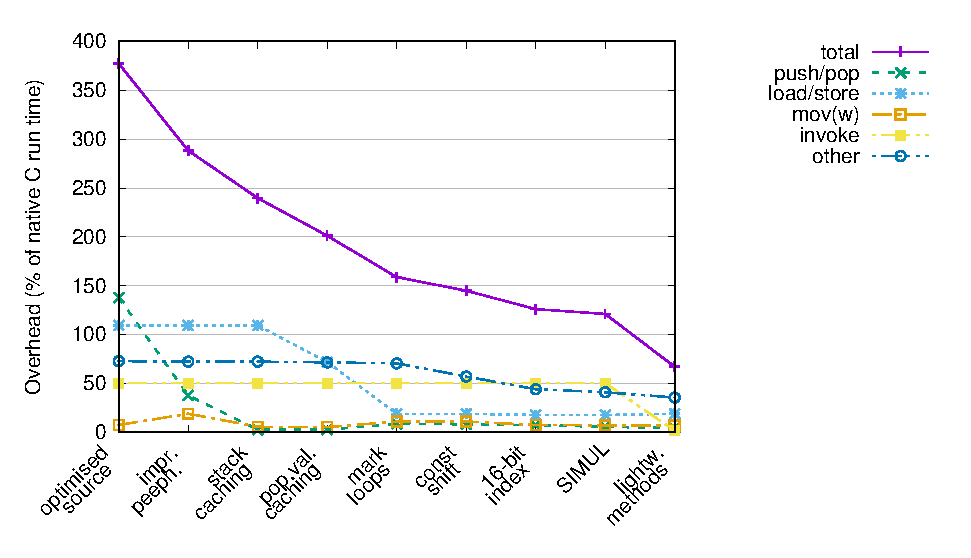
\includegraphics[width=\mygraphsize]{performance-per-opcode-category3a.eps}
\caption{Performance overhead per category}
\label{fig-performance-per-opcode-category}
\end{figure}

\begin{figure}
\centering
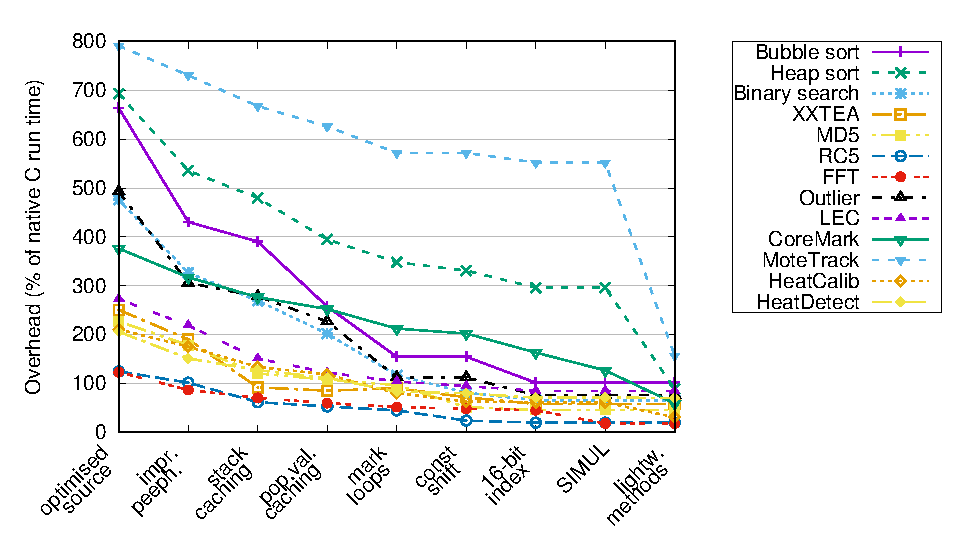
\includegraphics[width=\mygraphsize]{performance-per-benchmark3a.eps}
\caption{Performance overhead per benchmark}
\label{fig-performance-per-benchmark}
\end{figure}

Using the baseline AOT compilation on the optimised sources, the types 1, 2 and 3 overhead are all significant, at 138\%,  109\%, and 73\% respectively, and the 50\% overhead in the VM is mainly spent on method calls since the overhead from allocating temporary objects is already removed by the source code optimisations. The basic approach does not have many reasons to emit a move, so in some cases the AOT version actually spends fewer cycles on move instructions than the C version, resulting in small negative values.  When we improve the peephole optimiser to include non-consecutive push/pop pairs, push/pop overhead drops by 100.2\% (of native C performance), but if the push and pop target different registers, they are replaced by a move instruction, and we see an increase of 11.5\% in move overhead. For a 16-bit register pair this takes 1 cycle (for a \mycode{MOVW} instruction), instead of 8 cycles for two pushes and two pops. The increase in moves shows most of the extra cases that are handled by the improved peephole optimiser are replaced by a move instead of eliminated, since the 11.5\% extra move overhead corresponds to a 92\% reduction in push/pop overhead.

Next stack caching is introduced to utilise all available registers and eliminate most of the push/pop instructions that cannot be handled by the peephole optimiser. As a result the push/pop overhead drops to nearly 0, and so does the move overhead since most of the moves introduced by the peephole optimiser, are also unnecessary when using stack caching.

Having eliminated the type 1 overhead almost completely, popped value caching is added to remove a large number of the unnecessary load instructions. This reduces the memory traffic significantly, as is clear from the reduced load/store overhead, while the other types remain stable. Adding the mark loops optimisation further reduces loads, and this time also stores, by pinning common variables to a register. But it uses slightly more move instructions, and the fact that fewer registers are available for stack caching means stack values are spilled to memory more often. While 53.0\% is saved on loads and stores, the push/pop and move overhead increase by 6.0\% and 5.6\% respectively.

Most of the push/pop and load/store overhead has now been eliminated and the type 3 overhead, unaffected by these optimisations, has become the most significant source of overhead. This type has many different causes, and only part of it can be eliminated with the instruction set optimisations. These optimisations, especially the 16-bit array index, also reduce register pressure, which results in a slight decrease in the other overhead types, although this is minimal in comparison. The \mybench{CoreMark} and \mybench{FFT} benchmarks are the only ones to do 16-bit to 32-bit multiplication, so the average performance improvement for \mycode{SIMUL} is small, but Table \ref{tbl-performance-per-benchmark} shows it is significant for these two benchmarks.

Finally, the lightweight optimisation could be applied to almost every method. Lightweight methods still incur some overhead, which will be discussed in more detail in Section \ref{sec-evaluation-method-invocation}, but since they do not call the VM, the time spent in the VM on method calls is effectively eliminated.

Combined, the optimisations to the AOT compilation process reduce performance overhead from 377\% to 67\% of native C performance.

\begin{tabular}{lrrrrrrrrrrrr}
\toprule
BENCHMARK                          & b.sort            &  h.sort           & b.srch            & fft               & xxtea             & md5               & rc5               & coremk            & \makebox[0.2mm]{}   & average           \\
\hline
\multicolumn{10}{l}{CODE SIZE (BYTES)} \\
% Take JVM, Native C and AOT original from results_0BASE_R___P__C0_A0_S0_G1
\xxt JVM                           &                78 &               140 &                91 &               493 &               384 &              2986 &               457 &              5719 &     &                   \\
\xxt Native C                      &               150 &               416 &               212 &              1214 &              1442 &              9458 &               910 &             10388 &     &                   \\
\xxt AOT original                  &               520 &              1170 &               616 &              2694 &              3780 &             29362 &              4074 &             33668 &     &                   \\
% Take AOT optimised from results_4MARK_R11_P7_C1_A1_S1_G1
\xxt AOT optimised                 &               344 &               738 &               450 &              1460 &              2268 &             14798 &              2140 &             25560 &     &                   \\
\hline
\multicolumn{10}{l}{CODE SIZE OVERHEAD BEFORE OPTIMISATIONS (\%)} \\
% Take this from main-code-size-graph.xlsx 
\xxt Total                         &             242.1 &             179.9 &             190.6 &             121.9 &             162.1 &             210.4 &             347.7 &             223.8 &     &             209.8 \\
  \xxxt push/pop                   & \xt          57.9 & \xt          61.2 & \xt          52.8 & \xt          55.7 & \xt         102.6 & \xt         133.1 & \xt         163.1 & \xt          74.5 &     & \xt          87.6 \\
  \xxxt load/store                 & \xt          89.5 & \xt          64.1 & \xt          69.8 & \xt          31.8 & \xt          28.4 & \xt          56.7 & \xt          67.9 & \xt          53.5 &     & \xt          57.7 \\
  \xxxt mov(w)                     & \xt           1.3 & \xt           1.4 & \xt           0.9 & \xt           0.3 & \xt           0.7 & \xt          -2.7 & \xt          -1.3 & \xt           1.4 &     & \xt           0.3 \\
  \xxxt other                      & \xt          93.4 & \xt          53.1 & \xt          67.0 & \xt          34.1 & \xt          30.4 & \xt          23.3 & \xt         118.0 & \xt          94.4 &     & \xt          64.2 \\
\multicolumn{10}{l}{CODE SIZE OVERHEAD REDUCTION PER OPTIMISATION (\%)} \\
\xxt Impr. peephole                &             -57.9 &             -41.1 &             -45.3 &             -26.5 &             -38.5 &             -54.3 &             -62.4 &             -30.7 &     &             -44.6 \\
\xxt Stack caching                 &             -13.1 &             -20.6 &             -24.5 &             -37.1 &             -56.1 &             -78.6 &            -106.4 &             -18.7 &     &             -44.4 \\
\xxt Pop. val. caching             &             -18.5 &             -27.8 &               0.0 &             -13.8 &              -6.2 &             -18.8 &             -17.8 &             -12.6 &     &             -14.4 \\
\xxt Mark loops                    &              -2.6 &              +4.8 &              +7.5 &              -5.9 &              +6.0 &              -1.1 &              -3.7 &              -3.8 &     &               0.2 \\
\xxt Const shift                   &               0.0 &              -2.4 &              -4.7 &              -5.3 &              +1.6 &              +4.0 &              -5.5 &              -1.1 &     &              -1.7 \\
\xxt 16-bit array index            &             -23.7 &             -16.2 &             -11.3 &             -13.0 &             -11.6 &              -5.1 &             -16.7 &              -8.8 &     &             -13.3 \\
\xxt SIMUL                         &               0.0 &               0.0 &               0.0 &               0.0 &               0.0 &               0.0 &               0.0 &              -2.3 &     &              -0.3 \\
\multicolumn{10}{l}{CODE SIZE OVERHEAD AFTER OPTIMISATIONS (\%)} \\
\xxt Total                         &             126.3 &              76.6 &             112.3 &              20.3 &              57.3 &              56.5 &             135.2 &             145.8 &     &              91.3 \\
  \xxxt push/pop                   & \xt          21.1 & \xt           5.7 & \xt           7.5 & \xt           0.0 & \xt          13.3 & \xt           0.0 & \xt           4.4 & \xt          19.4 &     & \xt           8.9 \\
  \xxxt load/store                 & \xt          31.6 & \xt          33.5 & \xt          47.2 & \xt           4.1 & \xt          14.8 & \xt          37.2 & \xt          25.3 & \xt          36.8 &     & \xt          28.8 \\
  \xxxt mov(w)                     & \xt           0.0 & \xt           3.8 & \xt           4.7 & \xt          -2.6 & \xt           2.5 & \xt          -1.8 & \xt          17.8 & \xt           5.4 &     & \xt           3.7 \\
  \xxxt other                      & \xt          73.7 & \xt          33.5 & \xt          52.8 & \xt          18.8 & \xt          26.6 & \xt          21.0 & \xt          87.7 & \xt          84.2 &     & \xt          49.8 \\
\bottomrule
\end{tabular}   


\section{AOT translation: code size}
\label{sec-evaluation-aot-translation-code-size}
Next we examine the effects of our optimisations on code size. Two factors are important here: the size of the VM itself and the size of the code it generates.

The size overhead for the generated code is shown in figures \ref{fig-codesize-per-opcode-category} and \ref{fig-codesize-per-benchmark}, again split up per instruction category and benchmark respectively. For the first three optimisations, the two graphs follow a similar pattern as the performance graphs. These optimisations eliminate the need to emit certain instructions, which reduces code size and improves performance at the same time.

The mark loops optimisation moves loads and stores for pinned variables outside of the loop. This reduces performance overhead by 41\%, but the effect on code size varies per benchmark: some are slightly smaller, others slightly larger.

For each variable that is live at the beginning of the loop, the VM emits the load before the mark loop block, so code size is only reduced if the variable is loaded more than once. Code size may actually increase if the value is then popped destructively, since this causes the VM to emit a \mycode{mov}. Stores follow a similar argument. Also, for small methods the extra registers used may mean we have to save more call-saved registers in the method prologue. Finally, we get the performance advantage for each run-time iteration, but the effect on code size, whether positive or negative, only once.

% \begin{figure}
%  \centering
%  \begin{minipage}{0.45\textwidth}
%   \centering
%   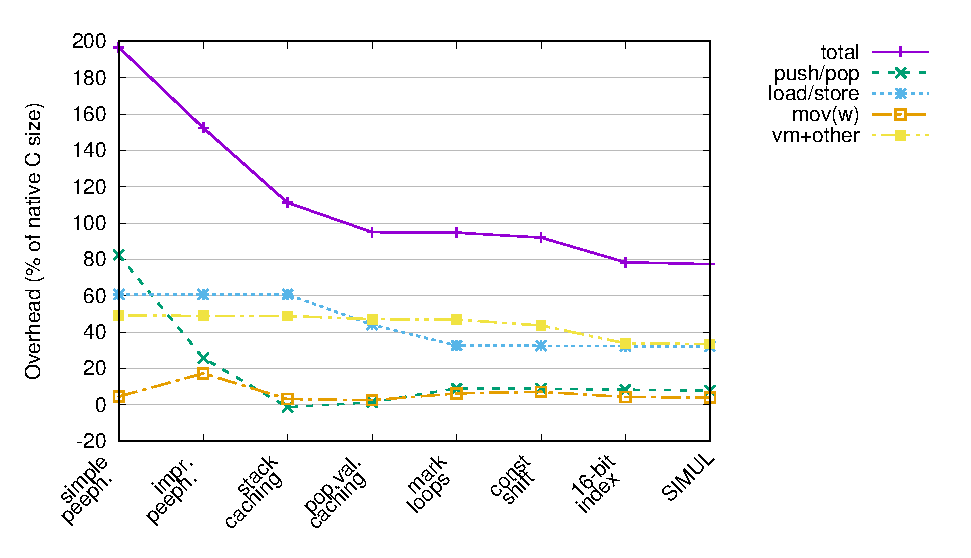
\includegraphics[width=\mygraphsize]{codesizeoverhead-per-opcode-category.eps}
%   \caption{Code size overhead per category}
%   \label{fig-codesize-per-opcode-category}
%  \end{minipage}\hfill
%  \begin{minipage}{0.45\textwidth}
%   \centering
%   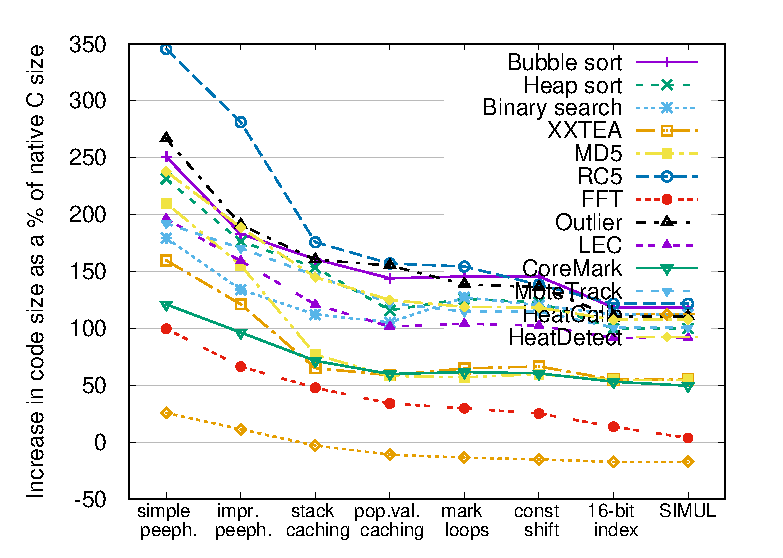
\includegraphics[width=\mygraphsize]{codesizeoverhead-per-benchmark.eps}
%   \caption{Code size overhead per benchmark}
%   \label{fig-codesize-per-benchmark}
%  \end{minipage}
% \end{figure}

\begin{figure}
\centering
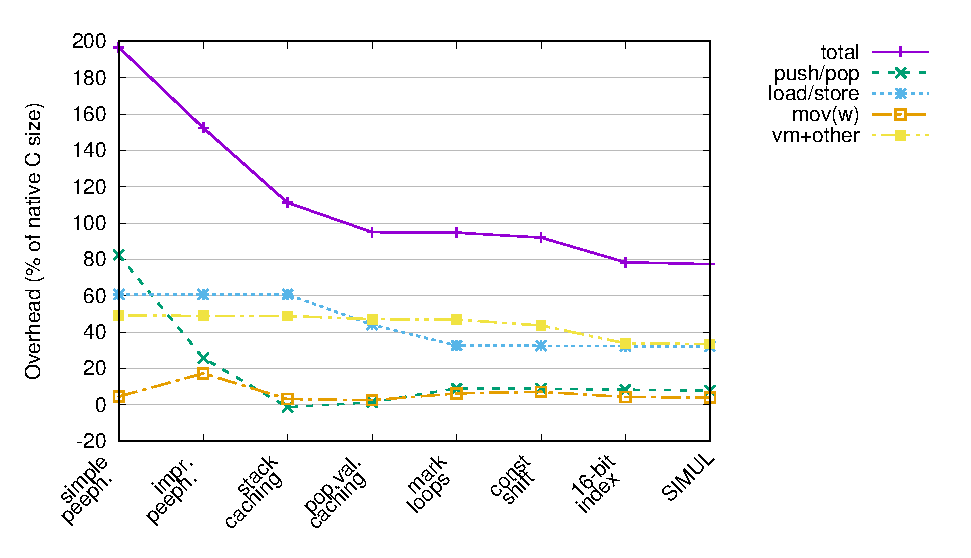
\includegraphics[width=\mygraphsize]{codesizeoverhead-per-opcode-category.eps}
\caption{Code size overhead per category}
\label{fig-codesize-per-opcode-category}
\end{figure}

\begin{figure}
\centering
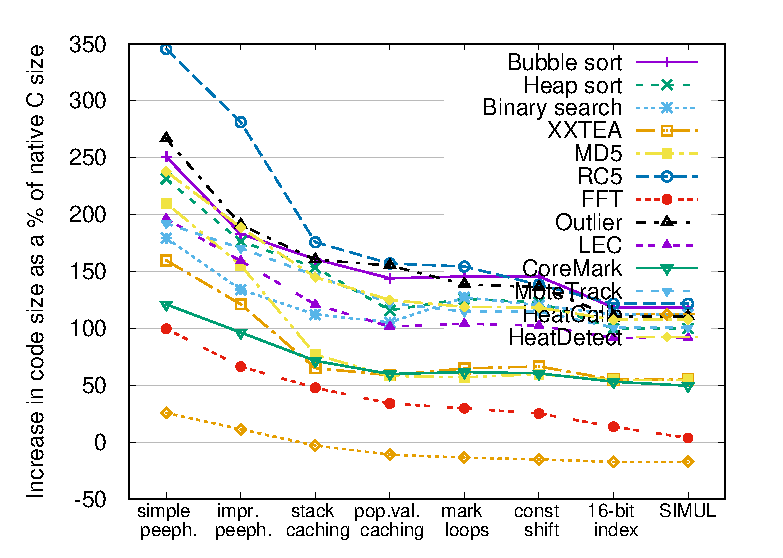
\includegraphics[width=\mygraphsize]{codesizeoverhead-per-benchmark.eps}
\caption{Code size overhead per benchmark}
\label{fig-codesize-per-benchmark}
\end{figure}

The constant shift optimisation unrolls the loop that is normally generated for bit shifts. This significantly improves performance, but the effect on the code size depends on the number of bits to shift by. The constant load and loop take at least 5 instructions. In most cases the unrolled shifts are smaller, but \mybench{MD5} and \mybench{XXTEA} show a small increase in code size since they contains shifts by a large number of bits.

Using 16-bit array indexes also reduces code size. The benchmarks here already have the manual code optimisations, so they use short index variables. This means the infuser emits \mycode{S2I} instructions to cast them to 32-bit ints if the array access instructions expect an int index. Not having to emit those when the array access instructions expect a 16-bit index, and the reduced work the access instruction needs to do, saves about 13\% code size overhead in addition to the 17\% reduction in performance overhead. Using 32-bit variables in the source code also removes the need for \mycode{S2I} instructions, but the extra effort needed to manipulate the 32-bit index variable makes the net code size even larger.

\subsection{VM code size and break-even point}
These more complex code generation techniques do increase the size of our compiler. The first column in Table \ref{tbl-code-size-and-memory-consumption} shows the difference in code size between the AOT translator and Darjeeling's interpreter. The basic AOT approach is 6605B larger than the interpreter, and each optimisation adds a little to the size of the VM.

They also generate significantly smaller code. The third column shows the reduction in the generated code size compared to the baseline approach. Here we show the reduction in total size, as opposed to the overhead used elsewhere, to be able to calculate the break-even point. Using the improved peephole optimiser adds 276 bytes to the VM, but it reduces the size of the generated code by 14.8\%. If we have more than 1.9KB available to store user programmes, this reduction will outweigh the increase in VM size. Adding more complex optimisations further increases the VM size, but compared to the baseline approach, the break-even point is well within the range of memory typically available on a sensor node, peaking at at most 18.3KB.

As is often the case, there is a tradeoff between size and performance. The interpreter is smaller than each version of our AOT compiler, and Table \ref{tbl-codesize-per-benchmark} shows JVM bytecode is smaller than both native C and AOT compiled code, but the interpreter's performance penalty may be unacceptable in many cases. Using AOT compilation we can achieve adequate performance, but the most important drawback has been an increase in generated code size. These optimisations help to mitigate this drawback, and both improve performance, and allow us to load more code on a node.

For the smallest devices, or if we want to be able to load especially large programmes, we may decide to use only a selection of optimisations to limit the VM size and still get both a reasonable performance, and most of the code size reduction. For example, dropping the markloop and constant shift optimisations would reduces the size of the VM by 3.6KB but keeps most of the reduction in generated code size, while performance overhead would increase to about 126\%.

% UPDATED 20180213

\begin{tabular}{lrrrrrr}
\toprule
                          & size vs     & size vs  &                      & AOT code  &   break & memory    \\
                          & interpreter & baseline &                      & reduction &   even  & usage     \\
\midrule
Baseline                  &     6605 B  &          &                      &           &         & 23 B      \\
Improved peephole         &     6881 B  &   276 B  & \scriptsize   (+276) &  -14.8\%  &  1.9 KB & 23 B      \\
Simple stack caching      &     7825 B  &  1220 B  & \scriptsize   (+944) &  -27.6\%  &  4.4 KB & 34 B      \\
Popped value caching      &     9057 B  &  2452 B  & \scriptsize  (+1232) &  -33.1\%  &  7.4 KB & 78 B      \\
Markloop                  &    12337 B  &  5732 B  & \scriptsize  (+3280) &  -33.0\%  & 17.4 KB & 85 B      \\
Const shift               &    12785 B  &  6180 B  & \scriptsize   (+448) &  -33.8\%  & 18.3 KB & 85 B      \\
16-bit array index        &    12765 B  &  6160 B  & \scriptsize    (-20) &  -38.2\%  & 16.1 KB & 85 B      \\
SIMUL                     &    12831 B  &  6226 B  & \scriptsize    (+66) &  -38.7\%  & 16.1 KB & 85 B      \\
Lightweight methods       &    13367 B  &  6762 B  & \scriptsize   (+536) &  -38.9\%  & 17.4 KB & 85 B      \\
\bottomrule
\end{tabular}

\subsection{VM memory consumption} The last column in Table \ref{tbl-code-size-and-memory-consumption} shows the amount of data that needs to be kept in memory while translating a method. We would like our VM to be able to load new code while other tasks are running concurrently. Here we only list the data that the VM would need to maintain in between receiving messages with new code since this is the amount of memory that would not be available to other tasks during this process. Of course new code is being processed, more stack memory is used, but this is freed a batch of instructions has been processed and can be reused by other applications.

For the baseline approach we only use 25 bytes for a number of commonly used values such as a pointer to the next instruction to be compiled, the number of instructions in the method, etc. The simple stack caching approach adds a 11 byte array to store the state of each register pair we use for stack caching. Popped value caching adds two more arrays of 16-bit elements to store the value tag and age of each value. Mark loops only needs an extra 16-bit word to mark which registers are pinned, and a few other variables. Finally, the instruction set optimisations do not require any additional memory. In total, our compiler requires 87 bytes of memory during the compilation process.

\subsection{Constant arrays}
%TODO write evaluation for constant arrays
TODO

\section{Benchmark details}
\label{sec-evaluation-benchmark-details}
Next, we have a closer look at some of the benchmarks and see how the effectiveness of each optimisation depends on the characteristics of the source code. The first section of Table \ref{tbl-performance-per-benchmark} shows the distribution of the bytecode instructions executed in each benchmark, and both the maximum and average number of bytes on the VM stack. We can see some important differences between the benchmarks. While the sort benchmarks on the left are almost completely load/store bounded, \mybench{XXTEA}, \mybench{RC5} and \mybench{MD5} are much more computation intensive, spending fewer instructions on loads and stores, and more on math or bitwise operations. The left three benchmarks and the \mybench{outlier detection} benchmark have only a few bytes on the stack, but as the benchmarks contain more complex expressions, the number of values on the stack increases.

The second part of tables \ref{tbl-performance-per-benchmark} and \ref{tbl-codesize-per-benchmark} first shows the overhead before optimisation, split up in the five instruction categories. We then list the effect of each optimisation on the total overhead. Finally we show the overhead per category after applying all optimisations.

The improved peephole optimiser and stack caching both target the push/pop overhead. Stack caching can eliminate almost all, and replaces the need for a peephole optimiser, but it is interesting to compare the two. The improved peephole optimiser does well for the simple benchmarks like sorting, \mybench{binary} search and \mybench{outlier detection}, leaving less overhead to remove for stack caching. The more computation intensive benchmarks contain more complicated expressions, which means there is more distance between a push and a pop, leaving more cases that cannot be handled by the peephole optimiser. For these benchmarks, replacing the peephole optimiser with stack caching yields a big improvement.

The benchmarks on the left spend more time on load/store instructions. This results in higher load/store overhead, and the two optimisations that target this overhead, popped value caching and mark loops, have a big impact. For the computation intensive benchmarks, the load/store overhead is much smaller, but the higher stack size means stack caching is very important for these benchmarks.

The smaller benchmarks highlight certain specific aspects of our approach, while the larger \mybench{CoreMark} benchmark covers a mix of different types of processing. As a result, it is an average case in almost every row in Table \ref{tbl-performance-per-benchmark}.
% The reason it ends up being the third slowest after all optimisations was discussed in \ref{sec-evaluation-coremark-non-automatic-optimisations}. With the non-automatic optimisations described there, \mybench{CoreMark}'s performance overhead would be 59\%, close to the average of the other benchmarks.

\subsubsection{Bubble sort}
\label{sec-evaluation-bubble-sort}
Next we look at \mybench{bubble sort} in some more detail. After optimisation, most of the stack related overhead has been eliminated and of the 101.2\% remaining performance overhead, most is due to other sources. For \mybench{bubble sort} there is a single, clearly identifiable source. The detailed trace output shows that 79.8\% is due to \mycode{ADD} instructions, but \mybench{bubble sort} hardly does any additions. This is a good example of how the simple JVM instruction set leads to less efficient code. To access an array we need to calculate the address of the indexed value, which takes one move and five additions for an array of shorts. This calculation is repeated for each access, while the C version is more efficient, using the auto-increment version of the AVR's LD and ST instructions to slide a pointer over the array. Of the remaining 101.2\% overhead, 93.1\% is caused by these address calculations.
% ADD, ADC and ADIW all cost 26.6\%. Each array access does 1 MOVW, 2 ADDs, 2 ADCs and 1 ADIW.
% 26.6*3+26.6/2 = 93.1

%\paragraph{Bit shifts} Interestingly, the reason \mybench{FFT} is the slowest, is similar to the reason \mybench{RC5} is fastest: they both spend a large amount of time doing bit shifts. \mybench{RC5} shifts by a variable, but large number of bits. Only 8.0\% of the executed bytecode instructions are bit shifts, but they account for 71\% of the execution time in the optimised version. For these variable bit shifts, our translator and \mycode{avr-gcc} generate a similar loop, so the two share a large constant factor.
%
%On the other hand \mybench{FFT} is a hard case because it does many constant shifts by exactly 6 bits. For these, our VM simply emits 6 single shifts, which is slower than the special case \mycode{avr-gcc} emits for shifts by exactly 6 bits.  While we could do the same, we feel this special case is too specific to include in our VM.

\subsubsection{HeatCalib and FFT}
Table \ref{tbl-codesize-per-benchmark} shows that after optimisation the \mybench{HeatCalib} benchmark has a negative code size overhead. This is caused by the fact that we compile the C versions using \mycode{avr-gcc}'s -O3 optimisations, optimising for performance instead of code size. In this case, as well as for \mybench{FFT}, this caused \mycode{avr-gcc} to duplicate a part of the code, which improves performance but at the cost of a significantly larger code size.

\subsubsection{MoteTrack}
The \mybench{MoteTrack} benchmark is by far the slowest of our benchmarks, at a 156\% overhead compared to native C. \mybench{MoteTrack} stores a database of reference signatures in flash memory. In C this is a complex struct containing a number of sub-structures and fixed-sized arrays, while it becomes a collection of objects and arrays in Java, shown in Figure \ref{fig-motetrack-refsignature-objects}.

Since the layout of the complete C structure is known at compile time, the C function to load a reference signature from its database can simply use \mycode{memcpy_P} to copy a block of 80 bytes from flash memory to RAM. For Java, the method to read from flash memory must follow multiple pointers to follow several indirections to find the locations to put each value. As a result, reading a single signature takes 1455 cycles in Java, and only 735 cycles in C.
% 68.5% overhead from reading refSignatures from flash. 68.5 / 1695 * 735 = 29.7

Additionally, the fixed offsets in the C structure means that accessing the reference signatures is also more efficient in C than in Java, which must follow a number of references to reach the data. We discuss this in more detail in Section \ref{sec-nested-data}.

\subsubsection{LEC}
In Section \ref{sec-introduction-performance} we calculated that the LEC compression algorithm reduced the energy spent to transmit our sample ECG data by 650 μJ, at the expense of 246 μJ spent on CPU cycles compressing the data, when implemented in C and using the ATmega128 CPU and CC2420 radio.

A compression algorithm like LEC is a good example of an optimisation that may be part of an application loaded onto a sensor node. However, if the overhead of using a VM is too high, the cost of compression may outweight the energy saved on transmission. Table \ref{tbl-performance-per-benchmark} shows that using the baseline AOT approach, the \mybench{LEC} benchmark has an overhead of 272.6\%. This means the CPU has to stay active longer, and compressing the data would cost $246 \mu J * 3.726 \approx 916 \mu J$, which is more than the 650 μJ saved on transmission.

After we apply our optimisations, the overhead is reduced to 84.6\%, resulting in $246 \mu J * 1.846 \approx 454 \mu J$ spent on compression. While the savings are less than when using native C to compress the data, our optimisations mean that in this scenario, we can save on transmission costs by using LEC compression, while using the baseline AOT approach, LEC compression would have resulted in a net loss.

\subsubsection{XXTEA and the mark loops optimisation}

\begin{figure}
\centering
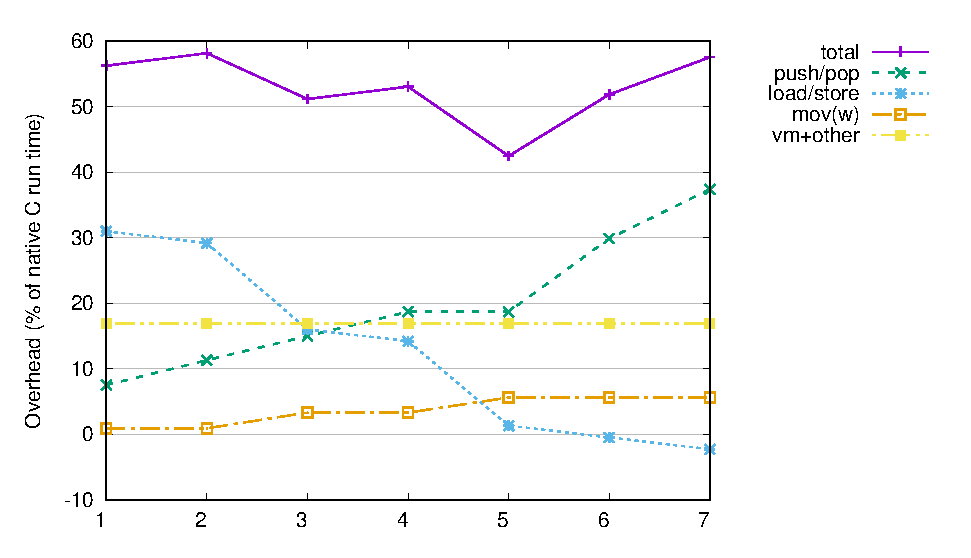
\includegraphics[width=\mygraphsize]{pinnedregs-performance-xxtea.eps}
\caption{XXTEA performance overhead for different number of pinned register pairs}
\label{fig-performance-pinnedregs-xxtea-per-opcode-category}
\end{figure}

\begin{figure}
\centering
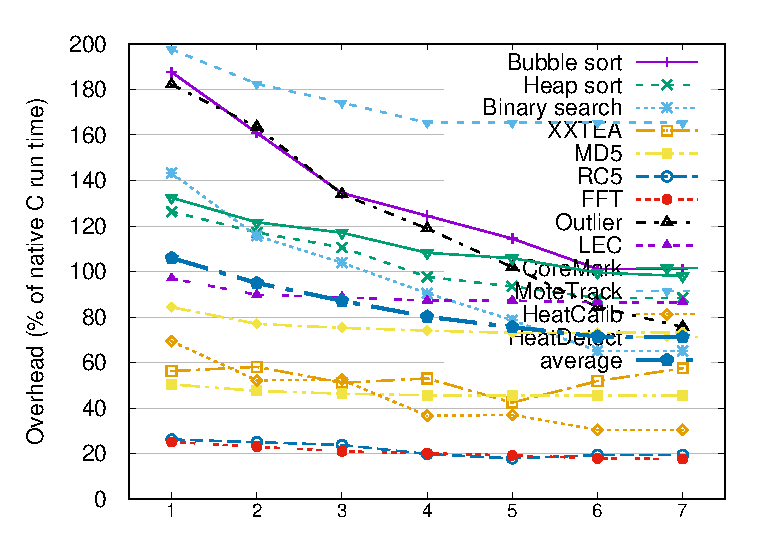
\includegraphics[width=\mygraphsize]{pinnedregs-performance-all-benchmarks.eps}
\caption{Per benchmark performance overhead different number of pinned register pairs}
\label{fig-performance-pinnedregs-per-benchmark}
\end{figure}

The \mybench{XXTEA} benchmark has the highest average stack depth of all benchmarks. As a result, popped value caching does not have much effect: most registers are used for real stack values, leaving few chances to reuse a value that was previously popped from the stack. 

When we apply the mark loops optimisation, performance actually degrades by 5\%! Here we have an interesting trade-off: if we use a register to pin a variable, accessing that variable will be cheaper, but this register will no longer be available for stack caching, so more stack values may have to be spilled to memory.

For most benchmarks, using the maximum of 7 register pairs to pin variables was also the best option. At a lower average stack depth, the fewer number of registers available for stack caching is easily compensated for by cheaper variable access. For \mybench{XXTEA} however, the cost of spilling more stack values to memory outweighs the gains of pinning more variables when too many variables are pinned. Figure \ref{fig-performance-pinnedregs-xxtea-per-opcode-category} shows the overhead for \mybench{XXTEA} from the different instruction categories. When we increase the number of register pairs used to pin variables from 1 to 7, the load/store overhead steadily decreases, but the push/pop and move overhead increase. For \mybench{XXTEA}, the optimum is at 5 pinned register pairs, at which the total overhead is only 43\%, instead of 58\% at 7 pinned register pairs.

Interestingly, when we pin 7 pairs, the AOT version does fewer loads and stores than the C compiler. Under high register pressure the C version may spill a register value to memory and later load it again, adding extra load/store instructions. When the AOT version pins too many registers, it will also need to spill values, but this adds push/pop instructions instead of loads/stores.

Figure \ref{fig-performance-pinnedregs-per-benchmark} shows the performance for each benchmark, as the number of pinned register pairs is increased. The benchmarks stay stable or even slow down when the number pinned pairs is increased beyond 5 are the benchmarks that have a high stack depth, while the benchmarks with low stack depth such as sort, \mybench{binary search} and \mybench{outlier detection} improve significantly. It should be possible to develop a simple heuristic to allow the VM to make a better decision on the number of registers to pin. Since our current VM always pins 7 pairs, we used this as our end result and leave this heuristic to future work.


\section{Constant arrays}
\label{sec-evaluation-const-array}
\begin{table}
\centering
\caption{Effect of constant arrays on size and performance}
\label{tbl-const-array}
	\scriptsize
    \centerline{
    \begin{tabular}{lrrrrrrrr} % UPDATED 20180327
    \toprule
                                & \multicolumn{2}{c}{RC5}   & \multicolumn{2}{c}{FFT}   & \multicolumn{2}{c}{LEC} & \multicolumn{2}{c}{MoteTrack} \\
Size of constant data           & \multicolumn{2}{c}{200}   & \multicolumn{2}{c}{2,048} & \multicolumn{2}{c}{51}  & \multicolumn{2}{c}{20,560}    \\
    \midrule
    \midrule
Using constant arrays           &       no &            yes &       no &            yes &        no &         yes &          no &             yes \\
Performance overhead            &   19.5\% &         19.5\% &   17.7\% &         17.7\% &    86.5\% &      84.6\% &  cannot run &         156.3\% \\
% Size in flash for @ConstArray version: 4 byte overhead per array for string table forward pointers and length fields
% Size in flash for _nca version       : the AOT size of the <clinit> taken from stdoutlog.txt
Size of constant data in flash  &     1998 &            204 &   26,714 &          2,052 &       930 &          59 &  cannot run &          20,588 \\
% 8 byte overhead per array for 5 byte heap header and 3 byte array header. MoteTrack would use 20,616 bytes if is could run.
Size of constant data in RAM    &      208 &              0 &    2,056 &              0 &        67 &           0 &  cannot run &               0 \\
    \bottomrule
    \end{tabular}
    }
\end{table}


Four benchmarks contain arrays of constant data, which were stored in flash memory by placing them in classes with the \mycode{@ConstArray} annotation. To evaluate the effect of this optimisation, we compare them to versions without this annotation. The results are shown in Table \ref{tbl-const-array}. There are three advantages to this optimisation: a small improvement in performance, reduced code size, and reduced memory usage.

When using constant arrays, the id of the array to read from is a bytecode parameter in the \mycode{GETCONSTARRAY} instruction. No reference to the array needs to be loaded on the stack, and the calculation to find the address of the target element is slightly easier, which results in a modest reduction in performance overhead of 1.9\% for the \mybench{LEC} benchmark.

The real advantage however, is the reduction in code size and memory usage. Without this optimisation, an array of constant data is transformed into normal bytecode that will create an array object on the heap and fill each element individually, as shown in Listing \ref{lst-constant-array-initialisation}.

The class initialiser uses four bytecode instructions per element to fill each element of the array. For an array of bytes, this can take up to 7 bytes of bytecode for each byte of data, which increases even further after AOT compilation. In the \mybench{LEC} benchmark this results in a class initialiser of 930 bytes, over \emph{18 times} the size of the original data. 

For such a small array this might still be acceptable, but the 26 KB needed to store \mybench{FFT}'s 2 KB of data is a significant overhead, and while \mybench{MoteTrack}'s 20 KB of data could fit in flash memory, the resulting class initialiser cannot. When using the constant array optimisation, the array is stored as raw data in the constant pool, resulting in just 4 bytes of overhead per array.

The final, and most significant advantage of this optimisation is that the array is no longer stored in RAM. Again, the 67 bytes of RAM needed to store \mybench{LEC}'s two constant arrays, each with 8 bytes overhead for the heap and array headers, may be acceptable. For \mybench{RC5} the 208 byte RAM overhead is starting to be significant, and while the \mybench{FFT} benchmark can still run without the constant array optimisation, its array consumes over half of the ATmega128's 4 KB of RAM. For \mybench{MoteTrack}, the size of its constant arrays is well over the amount of RAM available, making it impossible to run this benchmark without the constant array optimisation.
\section{Method invocation}
\label{sec-evaluation-method-invocation}
\begin{table}
\caption{Methods per benchmark and relative performance for normal, lightweight invocation, and inlining}
\label{tbl-evaluation-method-calls}
    \scriptsize
    \begin{threeparttable}
    \begin{tabular}{lllllll} % UPDATED 20180327
    \toprule
                                 & \# calls                 & C                & Java                          & Java                          & Java                            \\
                                 &                          &                  & Base version                  & Alternative version           & Using normal method calls       \\
    \midrule
    \midrule
    \\
    \mybench{CoreMark} \\
    ee\_isdigit                  & \multicolumn{1}{r}{3920} & normal (inlined) & manually inlined              & \tblhl lightweight (handw.)   & manually inlined                \\
    core\_state\_transition      & \multicolumn{1}{r}{1024} & normal           & lightweight                   & lightweight                   & \tblhl normal            \\
    crcu8                        & \multicolumn{1}{r}{584}  & normal (inlined) & manually inlined              & manually inlined              & manually inlined                \\
    crcu16                       & \multicolumn{1}{r}{292}  & normal           & lightweight                   & lightweight                   & \tblhl normal            \\
    calc\_func                   & \multicolumn{1}{r}{223}  & normal           & lightweight                   & lightweight                   & \tblhl normal            \\
    compare\_idx                 & \multicolumn{1}{r}{209}  & normal (inlined) & Proguard inlined              & Proguard inlined              & Proguard inlined                \\
    core\_list\_find             & \multicolumn{1}{r}{206}  & normal           & lightweight                   & lightweight                   & \tblhl normal            \\
    compare\_complex             & \multicolumn{1}{r}{110}  & normal           & Proguard inlined              & Proguard inlined              & Proguard inlined                \\
    crcu32                       & \multicolumn{1}{r}{64}   & normal           & lightweight                   & lightweight                   & \tblhl normal            \\
    matrix\_sum                  & \multicolumn{1}{r}{16}   & normal           & lightweight                   & lightweight                   & \tblhl normal            \\
    others (<16 calls each)      & \multicolumn{1}{r}{39}   & normal           & normal                        & normal                        & normal                          \\
    \\
    % The cycles from the simulation are for 50 iterations. Just divide by 50 here so the cycle count + the number of invokes produces the right overhead. An actual simulation run with 1 iteration is a bit slower, but only a few % so it is not significant enough to worry about here.
    %                                                                                 coremk                          coremk_lw                         coremk_fn
    \emph{cycles}                &                          &                  & \multicolumn{1}{r}{2,705,654} & \multicolumn{1}{r}{2,863,302} & \multicolumn{1}{r}{3,855,242}   \\
    \emph{overhead v native C}   &                          &                  & \multicolumn{1}{r}{58.9\%}    & \multicolumn{1}{r}{68.2\%}    & \multicolumn{1}{r}{126.4\%}     \\
    \emph{code size}             &                          &                  & \multicolumn{1}{r}{8990}      & \multicolumn{1}{r}{9006}      & \multicolumn{1}{r}{9,328}       \\
    \\
    \midrule
    \\
    \mybench{FFT} \\
    FIX\_MPY                     & \multicolumn{1}{r}{768}  & marked inline    & manually inlined              & \tblhl lightweight(handw.)    & \tblhl normal            \\
    \\
    %                                                                                 fft                             fft_lw                            fft_fn
    \emph{cycles}                &                          &                  & \multicolumn{1}{r}{179,692}   & \multicolumn{1}{r}{215,020}   & \multicolumn{1}{r}{661,360}     \\
    \emph{overhead v native C}   &                          &                  & \multicolumn{1}{r}{17.7\%}    & \multicolumn{1}{r}{40.8\%}    & \multicolumn{1}{r}{333.1\%}     \\
    \emph{code size}             &                          &                  & \multicolumn{1}{r}{1,342}     & \multicolumn{1}{r}{1,320}     & \multicolumn{1}{r}{1,408}       \\
    \\
    \midrule
    \\
    \mybench{heap sort} \\
    SWAP                         & \multicolumn{1}{r}{1642} & \#define         & manually inlined              & manually inlined              & manually inlined                \\
    siftDown                     & \multicolumn{1}{r}{383}  & normal           & lightweight                   & \tblhl manually inlined       & \tblhl normal            \\
    \\
    %                                                                                 hsort16                         hsort16_cht                       hsort16_fn
    \emph{cycles}                &                          &                  & \multicolumn{1}{r}{208,239}   & \multicolumn{1}{r}{184,071}   & \multicolumn{1}{r}{437,264}     \\
    \emph{overhead v native C}   &                          &                  & \multicolumn{1}{r}{88.5\%}    & \multicolumn{1}{r}{66.6\%}    & \multicolumn{1}{r}{295.8\%}     \\
    \emph{code size}             &                          &                  & \multicolumn{1}{r}{596}       & \multicolumn{1}{r}{662}       & \multicolumn{1}{r}{602}         \\
    % Data for hsort32:
    % \emph{cycles}              &                          &                  & \multicolumn{1}{r}{289,268}   & \multicolumn{1}{r}{286,200}   & \multicolumn{1}{r}{568,889}     \\
    % \emph{overhead v native C} &                          &                  & \multicolumn{1}{r}{66.2\%}    & \multicolumn{1}{r}{64.4\%}    & \multicolumn{1}{r}{226.8\%}     \\
    % \emph{code size}           &                          &                  & \multicolumn{1}{r}{702}       & \multicolumn{1}{r}{890}       & \multicolumn{1}{r}{722}         \\
    \bottomrule
    \end{tabular}
    \begin{tablenotes}
        \item Highlights indicate changes from the versions used to obtain the results in the previous sections.
    \end{tablenotes}
    \end{threeparttable}
\end{table}


In this section we will examine the effect of the lightweight method, compared to inlined code and normal method calls.

Most of our smaller benchmarks consist of only a single method. ProGuard automatically inlines methods only called from a single location, eliminating all method calls in the \mybench{LEC} benchmark. We will examine the effect of lightweight methods using the \mybench{FFT}, \mybench{Heap sort}, and \mybench{CoreMark} benchmarks.
\mybench{FFT} contains a single function, \mycode{fix_mpy}, which was inlined by the C compiler, so we manually inlined it in the Java version. \mybench{Heap sort} contains a real method call: it consist of two loops, both repeatedly calling the \mycode{siftDown} method. Since it is called from two places, and larger than ProGuard's size threshold, it is not automatically inlined. \mybench{CoreMark} is a much more extensive benchmark, and consists of many methods.

Table \ref{tbl-evaluation-method-calls} lists the functions of the \mybench{CoreMark}, \mybench{FFT} and \mybench{heap sort} benchmarks, and the number of times they are called in a single run. Next, we list the way they are implemented in C. \mybench{CoreMark} only defines normal functions, which are inlined by \mycode{avr-gcc} in three cases. \mybench{FFT}'s \mycode{fix_mpy} function is marked with the \mycode{inline} compiler hint, which was followed by \mycode{avr-gcc}. Finally \mybench{heap sort} uses just one extra function, and a macro to swap two array elements.

The Java base version column shows the way these functions are implemented in the Java versions of our benchmarks. We manually inlined C macros, and the functions that were inlined by the C compiler. The most commonly called methods were transformed to lightweight methods, simply by adding the \mycode{@Lightweight} annotation where possible. For the Java versions of the \mycode{compare_idx} and \mycode{compare_complex} methods, this was not possible since lightweight virtual methods are not supported.

In the next two columns we vary these choices slightly to examine the effect of lightweight methods.

For the \mybench{CoreMark} benchmark, we first replace the inlined implementation of the most frequently called method with a lightweight version. \mycode{ee_isdigit} returns true if a \mycode{char} passed to it is between \mycode{'0'} and \mycode{'9'}. Since this is a very trivial method, we manually wrote the bytecode for this lightweight method to use only the stack and no local variables. This slowed down the benchmark by 5\%, adding 170,493 cycles. Since the method is called 3920 times, this corresponds to an overhead of about 43 cycles, which is on the high side for such a small method.

This is due to another overhead from using a lightweight method that's hard to quantify: the boolean result of \mycode{ee_isdigit} is used to decide an \mycode{if} statement. When we inline the code, the VM can directly branch on the result of the expression \mycode{(c>='0' && c<='9')}, but the lightweight method first has to return a boolean, which is then tested after the lightweight call returns.

Next, we see what the performance would be without lightweight methods, and all methods, except the manually inlined \mycode{ee_isdigit} and \mycode{crcu8}, have to be implemented as normal Java methods. This adds a total of 1,135,373 cycles, making it 1.34 times slower than the lightweight methods version. Spread over 1,822 calls, this means the average method invocation added over 623 cycles, which is within the range predicted in Section \ref{sec-optimisations-method-calls}.

The \mybench{FFT} benchmark has a much lower running time than \mybench{CoreMark,} but still does 768 function calls. In the C and normal Java versions these are inlined. When we change \mycode{FIX_MPY} to a normal Java method, it is too large for ProGuard to inline. Using a handwritten lightweight method, the large number of calls relative to the total running time means the average overhead of over 46 cycles per invocation slows down the benchmark by 20\%. Without lightweight methods, the overhead would be 627 per call, slowing down the benchmark by 268\%.

Finally, for the \mybench{heap sort} benchmark we normally use a lightweight method for \mycode{siftDown}. While manually inlining it is possible, it is not an attractive option since the \mycode{siftDown} method is much more complex than \mycode{FIX_MPY} or \mycode{ee_isdigit}. When we do inline it, we see that the lightweight method adds some overhead compared to the inlined version, but much less than a normal method call would.

In terms of code size, using normal methods take slightly more space than a lightweight method. Listing \ref{lst-comparison-lightweight-and-normal-invocation} showed that the invocation is more complex for normal methods, and in addition the method prologue and epilogue are longer.

The difference between inlining and lightweight methods is less clear. For the smallest of methods, such as \mybench{CoreMark}'s \mycode{ee_isdigit}, the inlined code is slightly smaller than the call, but the \mybench{heap sort} benchmark shows that inlining larger methods can result in significantly larger code. Since \mycode{siftDown} is called from two places, duplicating it leads to a 11\% increase for the 16-bit version of \mybench{heap sort}. For the 32-bit version, where \mycode{siftDown} is relatively larger, this increases to 27\%.

As these three examples show, using lightweight methods gives us an option in-between a normal method call and inlining. This avoids most of the overhead of a normal method call, and the potential size increase of inlining.



\clearpage
\newgeometry{margin=1cm}
\thispagestyle{empty}
\begin{landscape}
\begin{table}[t!]
\caption{Cost of safety guarantees}
\label{tbl-safety-cost}
    \begin{tabular}{lrrrrrrrrrrrrrrr} % UPDATED 20180305
    \toprule
                                        & B.sort     &  H.sort    & Bin.Search & XXTEA      & MD5        & RC5        & FFT        & Outlier    & LEC        & CoreMark   & MoteTrack  & HeatCalib  & HeatDetect & \makebox[0.2mm]{} &   average \\
    \midrule
    \midrule
    \multicolumn{10}{l}{EXECUTED BYTECODE INSTRUCTIONS (\% of total executed bytecode instructions)} \\
    Array element/object field STORES   &       18.0 &        7.8 &        0.0 &        2.9 &        4.5 &        1.5 &        6.1 &        5.8 &        3.7 &        2.6 &       10.0 &        1.4 &        4.7 &                   &       5.3 \\
    Array element/object field LOADS    &       18.0 &       15.9 &        7.1 &        8.6 &        6.2 &        6.4 &        7.0 &       10.7 &        7.9 &       11.6 &       21.4 &        4.1 &        9.8 &                   &      10.4 \\
    \multicolumn{10}{l}{PERFORMANCE OVERHEAD VS NATIVE C (\% of native C)} \\
    unsafe                              &      101.2 &       88.5 &       65.2 &       57.6 &       45.7 &       19.5 &       17.7 &       75.7 &       84.6 &       97.0 &      156.3 &       30.5 &       73.4 &                   &      70.2 \\
    safe writes                         &      247.5 &      153.9 &       65.2 &       68.2 &       60.3 &       22.2 &       30.3 &      128.4 &      118.4 &      124.0 &      266.1 &       33.9 &       91.3 &                   &     108.4 \\
    safe reads and writes               &      393.9 &      287.8 &      151.7 &      100.0 &       80.3 &       33.4 &       43.0 &      226.6 &      179.8 &      202.2 &      445.1 &       43.9 &      126.9 &                   &     178.0 \\
    \multicolumn{10}{l}{PERFORMANCE OVERHEAD VS UNSAFE VM (\% of unsafe AOT)} \\
    safe writes                         &       72.7 &       34.7 &        0.0 &        6.7 &       10.0 &        2.3 &       10.7 &       30.0 &       18.3 &       13.7 &       42.8 &        2.6 &       10.3 &                   &      22.4 \\
    safe reads and writes               &      145.5 &      105.7 &       52.4 &       26.9 &       23.7 &       11.6 &       21.5 &       85.9 &       51.6 &       53.4 &      112.7 &       10.3 &       30.9 &                   &      63.3 \\
    \multicolumn{10}{l}{CODE SIZE OVERHEAD VS NATIVE C (\% of native C)} \\
    unsafe                              &      118.6 &      100.0 &      112.3 &       55.1 &       54.9 &      121.8 &        2.5 &      110.5 &       88.6 &       50.7 &      117.1 &      -17.2 &      107.7 &                   &      78.7 \\
    safe writes                         &      125.4 &      105.4 &      112.3 &       56.2 &       55.7 &      125.3 &        5.0 &      118.9 &       94.3 &       54.5 &      125.4 &      -16.4 &      114.7 &                   &      82.8 \\
    safe reads and writes               &      132.2 &      113.4 &      117.8 &       60.1 &       59.1 &      132.3 &        8.0 &      123.2 &      102.9 &       61.8 &      145.3 &      -13.9 &      118.5 &                   &      89.3 \\
    \multicolumn{10}{l}{CODE SIZE OVERHEAD VS UNSAFE VM (\% of unsafe AOT)} \\
    safe writes                         &        3.1 &        2.7 &        0.0 &        0.7 &        0.5 &        1.6 &        2.4 &        4.0 &        3.0 &        2.5 &        3.8 &        1.0 &        3.4 &                   &       2.3 \\
    safe reads and writes               &        6.2 &        6.7 &        2.6 &        3.2 &        2.7 &        4.7 &        5.4 &        6.0 &        7.6 &        7.4 &       13.0 &        4.0 &        5.2 &                   &       5.9 \\
    \bottomrule
    \end{tabular}
\end{table}
\end{landscape}
\clearpage
\restoregeometry


\section{The cost of safety}
\label{sec-evaluation-safety}

The advantage of using a VM to provide safety is that the necessary checks are easy to do, compared to native code, and most can be done at translation time. This leads to both a very modest increase in VM complexity due to the safety checks, and a lower run-time overhead. 
% would be nice to get code size for Harbor and t-kernel.

\subsection{Run-time cost}
\label{sec-evaluation-run-time-cost}

\begin{figure}
\centering
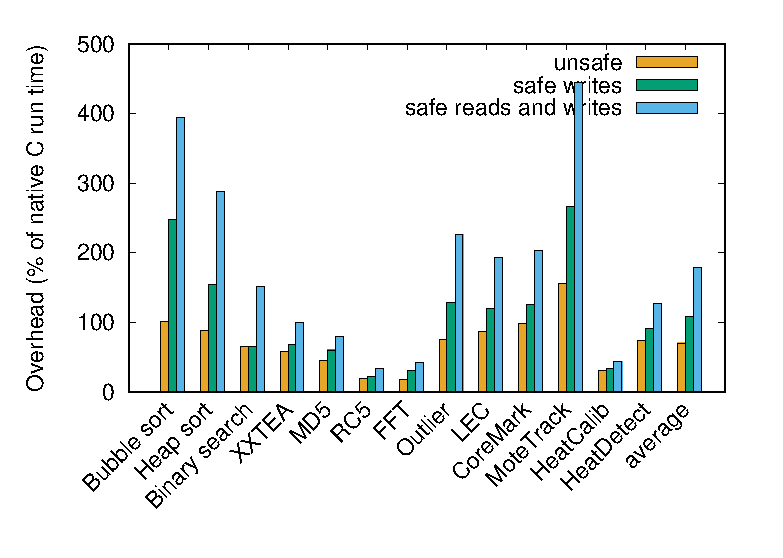
\includegraphics[width=\mygraphsize]{safety-cost.eps}
\caption{Overhead increase due to safety checks}
\label{fig-safety-cost-per-benchmark}
\end{figure}

\begin{figure}
\centering
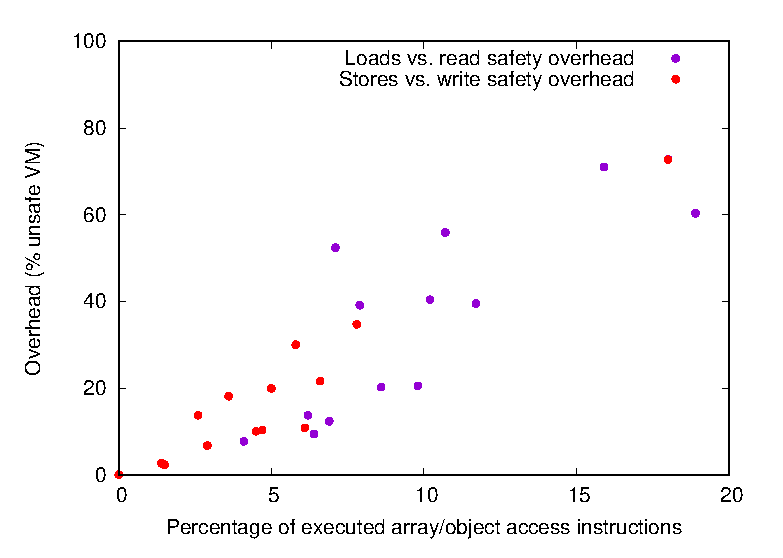
\includegraphics[width=\mygraphsize]{safety-ld-st-percentage-vs-overhead.eps}
\caption{Percentage of array/object load/store instructions and cost of read/write safety}
\label{fig-safety-ld-st-percentage-vs-overhead}
\end{figure}

\begin{figure}
\centering
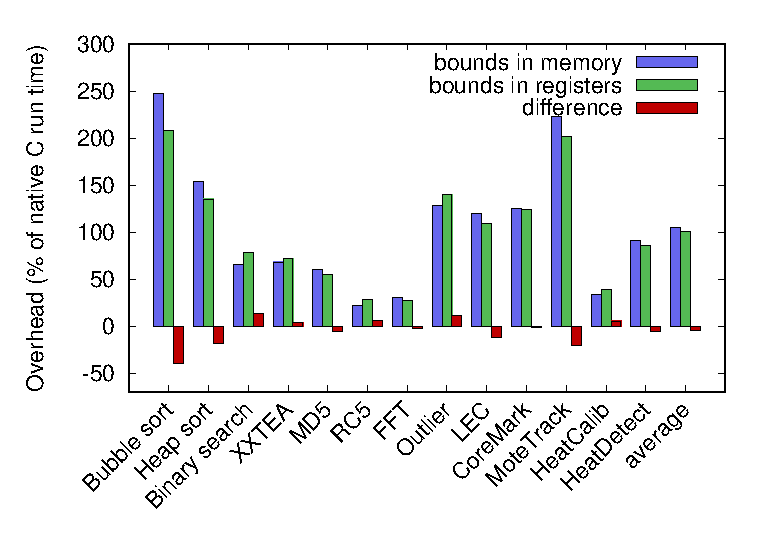
\includegraphics[width=\mygraphsize]{safety-cost-diff-using-regs.eps}
\caption{Comparison of safety cost with heap bounds in memory or registers}
\label{fig-safety-cost-memory-or-registers}
\end{figure}

Table \ref{tbl-safety-cost} shows the increase in performance and code size overhead as a result of the run-time safety checks for our 12 benchmarks. The performance overhead is also shown in Figure \ref{fig-safety-cost-per-benchmark}. The baseline here is the unsafe version of our VM, which is on average 67.0\% slower than native C. Adding write checks is sufficient to satisfy our guarantee that no malicious code can corrupt the state of the VM. This increases the average overhead to 104.6\% of native C, corresponding to a 22.5\% increase in run time compared to the unsafe VM.

The cost of the run-time safety checks depends greatly on the benchmark we run. Most checks are done at translation time, including writes to local and static variables. The only check that adds significant run-time overhead is check \ref{chk-memory-access-within-heap}, which checks the target of an object field or array write is within the bounds of the heap.

Thus, the run-time overhead is determined by the number of object or array accesses a benchmark does. The percentage of these is shown in the first part of Table \ref{tbl-safety-cost}. Since \mybench{bubble sort} has by far the highest percentage of array writes, at 18\% of all executed bytecode instructions, it also incurs the highest overhead from adding write safety, and slows down by 72.7\%. \mybench{Binary search} on the other hand, which does no writes at all, is unaffected. As usual \mybench{CoreMark}, being a large benchmark with a mix of operations, is somewhere in the middle. The correlation between the percentage of array and object writes, and the slowdown compared to the unsafe version is shown in Figure \ref{fig-safety-ld-st-percentage-vs-overhead}.

\subsubsection{Safe reads}
Up to this point the VM only checks the application cannot \emph{write} to memory it is not supposed to write to, however, it may still \emph{read} from any location.

The recently published Meltdown and Spectre vulnerabilities in desktop CPUs can be exploited by malicious code to read from anywhere in memory, exposing both kernel's and other applications private data, which may contain sensitive information such as authentication tokens, passwords, etc. This sent OS vendors rushing to release patches, which early report suggest may cause a performance penalty of up to 11\% \cite{Simakov:2018wp}.

Whether this is also a problem on a sensor node depends on the scenario. If the VM or other tasks contain sensitive information, then this may need to be protected. However, in many sensor node applications the node may only be running a single application, and the VM does not contain any state that would be useful to an attacker. In these cases, write safety will be sufficient.

Adding read safety to our VM is trivial: instructions to load local and static variables are already protected since they use the same code to access a variable as the store instructions. For heap access, we simply add the same call to \mycode{heapcheck} to the \mycode{GETARRAY} and \mycode{GETFIELD} instructions just before the actual read.

Figure \ref{fig-safety-cost-per-benchmark} shows the cost of providing read safety is higher than write safety. Most applications read from an array or object much more frequently than they write to them. As a result, our VM with read and write safety turned on slows down by 64\% on average, corresponding to a 174\% slowdown over native C. In addition to the sort benchmarks, \mybench{MoteTrack} also suffers greatly from adding read safety, since it spends 21\% of its instructions reading from the objects and arrays, mostly from the RSSI signature database. \mybench{RC5} is the fastest benchmark, since it not only does relatively few array reads and writes, but also spends a large amount of time on expensive variable bit shifts, which have identical performance in both C and AOT compiled versions. The result is a slowdown of only 33\% compared to native C for the fully safe version.

\subsubsection{Keeping heap bounds in registers}
In Section \ref{sec-safety-heap-access} several alternatives for the heap bounds check were considered, one of which is to keep the bounds in dedicated registers to avoid having to fetch them from memory for each check. Here we evaluate this choice.

Having the bounds in registers would reduce the cost of the check from 22 to 14 cycles, reducing the overhead of safety checks by $8/22 \approx 36\%$. However, this uses 4 registers which we cannot use for stack caching.

To estimate how this would affect performance, the benchmarks were run using the unsafe VM, with the number of registers available to the stack cache reduced by 4. Since this does not affect the number of heap accesses, we then added the observed overhead for safety checks, reduced by 36\%.

Figure \ref{fig-safety-cost-memory-or-registers} shows the overhead for our chosen approach with the heap bounds in memory, compared to the expected overhead when the heap bounds are stored in registers. For some benchmarks such as \mybench{bubble sort} and \mybench{MoteTrack}, the savings in heap bounds checks outweighs the reduced effectiveness of the stack cache. But the improvement in performance is relatively small, and for other benchmarks the reverse is true, showing minor slowdowns when heap bounds are kept in registers. On average the benchmarks are quite balanced, as is the larger \mybench{CoreMark} benchmark.

As future work we may consider using some basic statistics, such as the percentage of array write instructions and average stack depth, to choose one of the two options on a per-method basis. But as usual there is a tradeoff, in this case VM size and complexity, which may not be worth the effort given the relatively small gains.

\subsection{Code-size cost}
Next, we examine the cost of safety in terms of code size. This comes in two parts: increased VM complexity and size, and an increase in the code it generates.

Most of our checks are no more complex than comparing two integers, and rejecting or terminating the application if a condition is not met. The most complex part is deciding the stack effects of instructions to guard against stack under- or overflow. This comes in the form of a table that encodes the effects of most instructions, and some specialised code to analyse a handful of instructions without fixed effect. In total, the increase in VM size for our safe version is a modest 1,468 bytes.

As we can see in Table \ref{tbl-safety-cost}, the size of the code the VM generates increases by only 2.4\% for write only safety and 6.0\% when reads are also protected. Since many checks occur at translation time, most instructions produce exactly the same native code in the safe version of our VM. The exceptions are \mycode{INVOKEVIRTUAL} and \mycode{INVOKEINTERFACE}, which now contain the expected stack effects to realise check \ref{chk-invokevirtual-stack-effects-match}, and the array and object write instructions \mycode{PUTFIELD} and \mycode{PUTARRAY}, that emit a single extra \mycode{CALL} instruction the \mycode{heapcheck} routine. Since these instructions are both relatively rare, and already generate a larger than average block of native instructions, the total effect on code size is limited.

\subsection{Comparison to native code alternatives}
As discussed in Section \ref{sec-state-of-the-art-safety}, several non-VM approaches have been proposed to guarantee safety on a sensor node. Two of these, \emph{t-kernel} \cite{Gu:2006ww} and Harbor \cite{Kumar:2007ge}, allow the node to guarantee safety independent of the host. Both target the Mica family of sensor nodes, which use the same ATmega128 CPU used by CapeVM. In this section we compare them to CapeVM and consider the question whether a VM is a good way to provide safety.

\emph{t-kernel} reports a slowdown of between 50 and 200\%, which is roughly in the same range as CapeVM. However both \emph{t-kernel} and CapeVM provide additional advantages. In \emph{t-kernel}'s case a form of virtual memory, and for the VM platform independence. This makes them hard to compare, but we note that while the performance of both systems is similar, \emph{t-kernel}'s code size overhead is much higher at a 6-8.5x increase, limiting the size of programmes that can be loaded onto the device.

A better comparison is possible for Harbor, which only provides safety. Harbor uses three benchmarks to evaluate performance: writing arbitrary data to an array to mimick copying a buffer of sensor data, and the \mybench{outlier detection}, and 16-bit \mybench{FFT} benchmarks also used in the rest of CapeVM's evaluation. The size of the data used for the first two is not specified in the paper, but since it mentions they work on sensor data and the ATmega CPU has 13-bit analog-to-digital converters, we use 16-bit data for these benchmarks as well.

As mentioned before, the \mybench{FFT} benchmark is taken from the Harbor sources \cite{sos-operating-system}, and \mybench{outlier detection} implemented as described in the paper. The \mybench{array writes} benchmark is implemented as a loop that fills an array of 256 elements with an arbitrary number, as shown in Listing \ref{lst-fill-array}.


\begin{listing}
\begin{minted}{java}
    for (short i = 0; i < NUMBERS; i++) {
        numbers[i] = (short)1;
    }
\end{minted}
\caption{Array writes benchmark (8-bit version)}
\label{lst-fill-array}
\end{listing}

\begin{table}
\caption{Comparison of overhead in Harbor and CapeVM}
\label{tbl-safety-overhead-harbor}
    \begin{tabular}{lrrrrrrr} % UPDATED 20180316
    \toprule
    Benchmark    & \makebox[3mm]{} & \multicolumn{3}{c}{CapeVM overhead} & \makebox[2mm]{} & \multicolumn{2}{c}{Harbor overhead} \\
    \\
                 &                 & VM      & + safety checks & = safe VM   &                 & current & hypothetical              \\
    \midrule
    \midrule
    Array writes &                 & 182.8\% & 268.7\%       & 451.5\%   &                 & 1230\%  & 416\%                     \\
    Outlier      &                 & 75.8\%  & 52.7\%        & 128.5\%   &                 & 690\%   & 234\%                     \\
    16-bit FFT   &                 & 17.7\%  & 12.6\%        & 30.3\%    &                 & 380\%   & 129\%                     \\
    \bottomrule
    \end{tabular}
\end{table}



The resulting overhead is shown in Table \ref{tbl-safety-overhead-harbor}. Filling an array is a hard case for safe CapeVM since consecutive array writes are expensive for two reasons: (i) it results in repeated executions of the \mycode{PUTARRAY} instruction, which calculates the target address for each write, while native code can slide a pointer over the array, and (ii) each of these writes will trigger a call to \mycode{heapcheck}.

CapeVM incurs overhead both related to the VM, and because of the added run-time safety checks, while for Harbor all overhead is due to safety checks. Still, CapeVM's total overhead of 451.5\% is much lower than Harbor's 1230\%.

While CapeVM is more than twice as fast as Harbor for this benchmark, the comparison is not entirely fair. Harbor lists the cycle overhead for all of its 5 run-time protection primitives. We assume that without any function calls, only the 'Write access check' is relevant to this benchmark, which takes 65 cycles. In contrast, CapeVM's \mycode{heapcheck} routine only takes 22 cycles.

The difference is due to Harbor's more fine grained protection, which allows it to grant access to any aligned block of 8 bytes to the application, while CapeVM's protection is more coarse. If Harbor could be modified to use a similar check, its overhead could potentially be reduced to $1230 / 65 * 22 \approx 416\%$, slightly faster than CapeVM's total overhead. However, it is not clear from the paper whether Harbor's architecture could support such a coarse-grained check since it requires all application data that needs run-time write checks to be in a single block of memory.

While this shows CapeVM achieves a performance comparable to even a hypothetical optimised version of Harbor, the \mybench{array writes} benchmark does not highlight the advantage of using a VM to provide safety because it spends most of its time writing to an array, for which both approaches insert a run-time check. However, the VM can verify writes to local and static variables to be safe at translation time, while the Harbor sources \cite{sos-operating-system} show that its verifier requires \emph{all} stores to go through the run-time write access check. The authors do note that static analysis of the code could reduce the number of checks, but that this would come at the cost of a significantly more complex verifier.

CapeVM's \emph{total} overhead for the \mybench{array writes} benchmark is slightly higher than the hypothetical optimised Harbor, but the overhead due to safety checks is lower because CapeVM does not need to check writes to the index variable \mycode{i}. This advantage should be more pronounced in code with more frequent writes to local variables, which is exactly the case for the more realistic \mybench{outlier detection} and \mybench{FFT} benchmarks. 

The reported overhead is 690\% and 380\%, which would result in 234\% and 129\% resp., when using the faster memory access check. For these benchmarks, CapeVM is significantly faster at only 128.5\% or 30.3\% overhead.

\section{Expected perfomance on other platforms}
\label{sec-evaluation-other-platforms}
Platform independence is one of the main advantages of using a VM. The AVR family of CPUs is widely used in low power embedded systems, and we implemented our VM for the ATmega128 CPU. However, our approach does not depend on any AVR specific properties and the approach described in this dissertation can be applied on other embedded CPU platforms to improve performance and provide a safe execution environment. The main requirements are the ability to reprogramme its own programme memory, and the availability of a sufficient number of registers for stack caching.

While it is impossible to determine exactly what the resulting performance would be on different platforms without porting the VM, we present some results here that indicate it is likely to be worse than the results we see on the ATmega.

Two parameter that are of important influence to our VM are the number of available registers and the size of the registers. Table \ref{tbl-ATmega-msp430-m0-registers} lists these parameter for the ATmega, and two other common families of embedded CPUs, the Texas Instruments MSP430 and ARM Cortex-M0. These CPUs are similar in many ways, including the amount of RAM and flash memory typically available, but differ in the number of registers and word size.

\begin{table}
\caption{Number or registers and word size for the ATmega, MSP430, and Cortex M0}
\label{tbl-ATmega-msp430-m0-registers}
    \begin{tabular}{lrrr} % NO SIMULATION DATA
    \toprule
                                           & ATmega       & MSP430     & Cortex M0 \\
                                           & \cite{Atmel:ATmega128Datasheet, Atmel:AVRInstructionSetManual}
                                           & \cite{TexasInstrumentsIncorporated:MSP430F1611Datasheet, TexasInstrumentsIncorporated:MSP430x1xxUsersGuide}
                                           & \cite{ARM:2009vz} \\
    \midrule
    \midrule
    Number of general purpose registers    & 32           & 12         & 13        \\
    Word size                              & 8-bit        & 16-bit     & 32-bit    \\
    Total register file size (bytes)       & 32           & 24         & 52        \\
    \bottomrule
    \end{tabular}
\end{table}

\subsection{Number of registers}

\begin{figure}
\centering
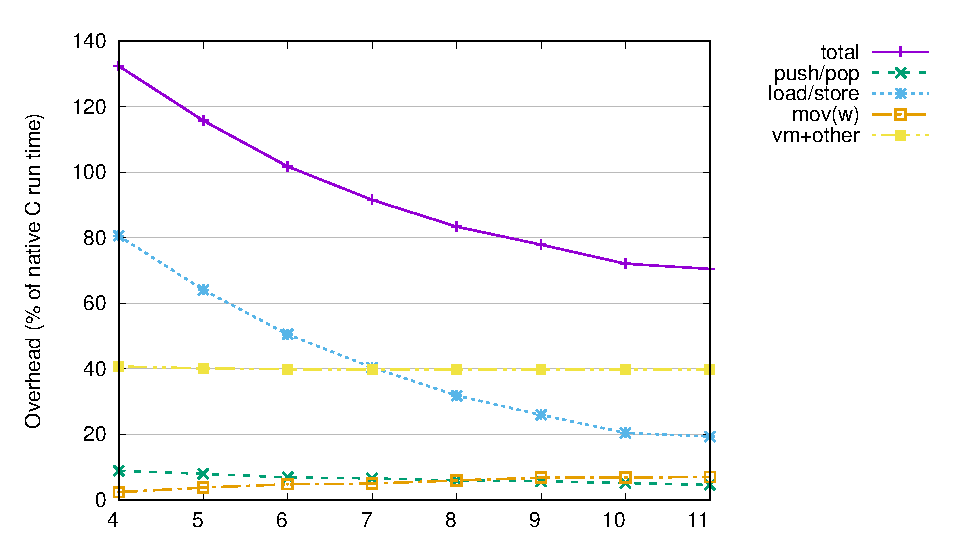
\includegraphics[width=\mygraphsize]{cachesize-performance-per-opcode-category.eps}
\caption{Performance for different stack cache sizes (in pairs of registers)}
\label{fig-performance-per-opcode-category-per-cachesize}
\end{figure}

\begin{table}
\caption{Performance overhead for different stack cache sizes (in pairs of registers)}
\label{tbl-performance-per-opcode-category-per-cachesize}
    \begin{tabular}{lrrrrrr} % UPDATED 20180327
    \toprule
    Number of                      & \multicolumn{5}{l}{Overhead} \\
    register pairs                 &  push/pop &   load/store &      mov(w) &    vm+other & \makebox[0.2mm]{}   &   total \\
    \midrule
    \midrule
      4                            &       8.7 &         80.5 &         2.4 &        38.1 &                     &   129.7 \\
      5                            &       7.8 &         64.0 &         3.8 &        37.5 &                     &   113.0 \\
      6                            &       6.7 &         50.3 &         4.7 &        37.0 &                     &    98.7 \\
      7                            &       6.4 &         40.2 &         4.9 &        37.0 &                     &    88.4 \\
      8                            &       5.7 &         31.6 &         5.8 &        36.9 &                     &    80.1 \\
      9                            &       5.5 &         25.6 &         6.7 &        36.9 &                     &    74.6 \\
     10                            &       4.9 &         20.1 &         6.8 &        36.9 &                     &    68.7 \\
     11                            &       4.3 &         18.9 &         6.9 &        36.9 &                     &    67.0 \\
    \bottomrule
    \end{tabular}
\end{table}


The ATmega has 32 8-bit registers available, which we manage as 16 pairs since our VM stores data in 16-bit slots. Looking at the MSP430, it only has 12 registers, but they are 16-bit. 5 register pairs are reserved on the ATmega, leaving us with 11 pairs available for stack caching. If we can achieve the same by reserving 5 16-bit registers on the MSP430, 7 registers will be available to the stack cache.

To evaluate the effect of a smaller number of registers on the stack cache, all benchmarks were run while restricting the number of registers the cache manage may use. Since our approach needs a minimum of 4 pairs, we vary the number of register from 4 to 11.

The results are shown in Figure \ref{fig-performance-per-opcode-category-per-cachesize} and Table \ref{tbl-performance-per-opcode-category-per-cachesize}. As is common with caching techniques, the first few registers have the most impact, with half of the overhead reduction already realised when adding the first two additional registers. Ignoring all other difference for the moment, the effect of reducing the number of register pairs from 11 to 7 is an increase in overhead by 21.1\%, to 91.3\%.

The Cortex M0 has one general purpose register more than the MSP430, and at 8 register pairs the overhead drops to 83.2\%. In addition, the M0's registers are 32-bit, which means in cases where mostly 32-bit values are used, the stack size is effectively doubled since values can be stored in a single register instead of two pairs of 8-bit registers.

A final interesting thing to note in Figure \ref{fig-performance-per-opcode-category-per-cachesize} is the fact the increasing the cache size mostly reduces the load/store overhead. Using only 4 pairs, stack caching has already removed most of the push/pop overhead, which only drops slightly when more registers are used. However, these extra registers reduce load/store overhead significantly since more registers are available for the markloop optimisation, and using more registers it increases the chance that an old, popped value may still be present, allowing popped value caching to eliminate more loads.

\subsection{Word size}
\label{sec-evaluation-other-platforms-word-size}

\begin{figure}
\centering
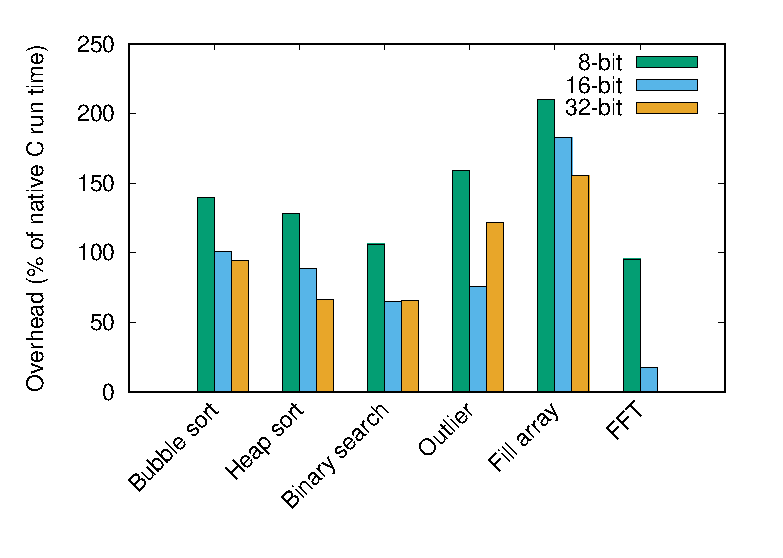
\includegraphics[width=\mygraphsize]{8_16_32_bit.eps}
\caption{Performance for different data sizes}
\label{fig-performance-8-16-32-bit}
\end{figure}

% UPDATED 20180214

\begin{table}[]
\centering
\caption{Performance for different data sizes}
\label{tbl-performance-8-16-32-bit}
\begin{tabular}{lrrr}
\toprule
               &   8-bit  &  16-bit  &     32-bit \\
\midrule
Bubble sort    &    139.5 &    101.2 &       94.4 \\
Heap sort      &    128.4 &     88.5 &       66.2 \\
Binary search  &    106.3 &     65.2 &         66 \\
Outlier        &      159 &     75.7 &      121.6 \\
FFT            &     96.7 &     17.7 &            \\
\bottomrule
\end{tabular}
\end{table}


A second important difference between the CPUs in Table \ref{tbl-ATmega-msp430-m0-registers} is the size of the registers. The main measure to evaluate our approach has been the overhead compared to native C performance or code size. While having a large register size is good for absolute performance, we expect it to hurt the \emph{relative} performance of our VM.

A number of benchmarks can be implemented using different data sizes. As mentioned in Section \ref{sec-evaluation-benchmarks}, 16-bit data is used in the main evaluation. Figure \ref{fig-performance-8-16-32-bit} and Table \ref{tbl-performance-8-16-32-bit} show the resulting performance for 8, 16, and 32-bit versions of these benchmarks (no 32-bit version of the \mycode{fix\_fft.c} code was available).

In almost all cases, a smaller data size results in a slower performance. This is because using larger data sizes increases the time spent in code that is common to both C and AOT versions. Taking \mybench{bubble sort} as an example, both versions do the same number of array loads, comparisons, and array stores. When operating on 32-bit data, this takes twice as long as for 16-bit data. In addition the AOT version introduces overhead, in \mybench{bubble sort}'s case primarily from calculating array element locations (see Section \ref{sec-evaluation-bubble-sort}). For a 32-bit array, this takes 17 cycles, 8 of which are spent on the actual load or store, but for 16-bit array access this is only 4 out of 13 cycles.

This effect is even clearer for more complex operations like multiplication. 16x16 to 16-bit multiplication can be implemented in a few instructions and only takes 10 cycles on the ATmega. 32x32 to 32-bit multiplication is implemented by calling \mycode{avr-gcc}'s \mycode{\_\_mulsi3} function, and takes 85 to 100 cycles.

Thus, working with 16-bit or 32-bit data on an 8-bit CPU helps the compiler's relative performance by introducing a larger common component that both C and AOT compiled versions have to execute. On the MSP430 or Cortex M0, that operate on 16-bit or 32-bit values in a single step, this effect will be reduced or eliminated. The exact impact of this is hard to estimate, but it is likely to be in the order of tens of percents extra overhead.

In Table \ref{tbl-performance-8-16-32-bit} we see the \mybench{outlier detection} benchmark performs worse for 32-bit data compared to 16-bit data. This is due to a mismatch between the infuser and ProGuard. In JVM bytecode, local variables are stored in 32-bit slots. The code generated by \mycode{javac} uses a separate slot for each variable, but ProGuard attempts to reduce memory consumption by mapping multiple variables to the same slot if their live ranges do not overlap. The infuser processes the ProGuard optimised code, as shown in Figure \ref{fig-translation-process}, and replaces the JVM's 32-bit operations by 16-bit versions where possible. In the 32-bit \mybench{outlier detection} benchmark, ProGuard mapped a 32-bit and 16-bit variable to the same slot, which prevents the infuser from using the cheaper 16-bit operations for this variable. This once again highlights the need for a unified, optimising compiler, combining the tasks of \mycode{javac}, ProGuard and the Darjeeling infuser.

The large difference in performance for \mybench{FFT} is mostly due to bit shifts. The 8-bit version does many shifts of a 16-bit value by exactly 6 bits. Our VM simply emits 6 single-bit shifts, while \mycode{avr-gcc} has a special optimised version for this case, which we considered too specific to include in our VM. The 32-bit version spends about half of its time shifting a 32-bit value by 15 bits, The VM and \mycode{avr-gcc} both implement this using the same loop, which again adds a large common factor, thus reducing the relative overhead.


%JVM_GETARRAY_I                                                  554880  18.2%  35.3%C      32640  17.0 |    1    24   7.8%  15.8%C 4->4:Int 
%1        movw r30, r6    -> 0x010E2E: movw r30, r6                32640                     32640
%1        add r30, r30    -> 0x010E30: add r30, r30                32640                     32640
%1        adc r31, r31    -> 0x010E32: adc r31, r31                32640                     32640
%1        add r30, r30    -> 0x010E34: add r30, r30                32640                     32640
%1        adc r31, r31    -> 0x010E36: adc r31, r31                32640                     32640
%1        add r30, r4     -> 0x010E38: add r30, r4                 32640                     32640
%1        adc r31, r5     -> 0x010E3A: adc r31, r5                 32640                     32640
%2        adiw r30, 3     -> 0x010E3C: adiw r30, 3                 65280                     32640
%
%2        ldpi r22, Z     -> 0x010E3E: ldpi r22, Z                 65280                     32640
%2        ldpi r23, Z     -> 0x010E40: ldpi r23, Z                 65280                     32640
%2        ldpi r20, Z     -> 0x010E42: ldpi r20, Z                 65280                     32640
%2        ld r21, Z       -> 0x010E44: ld r21, Z                   65280                     32640
%overhead: 9, load 8
%
%JVM_GETARRAY_S                                                  359040  18.2%  36.6%C      32640  11.0 |    1    16   6.2%  13.6%C 4->2:Short 
%1        movw r30, r6    -> 0x010DF2: movw r30, r6                32640                     32640
%1        add r30, r30    -> 0x010DF4: add r30, r30                32640                     32640
%1        adc r31, r31    -> 0x010DF6: adc r31, r31                32640                     32640
%1        add r30, r4     -> 0x010DF8: add r30, r4                 32640                     32640
%1        adc r31, r5     -> 0x010DFA: adc r31, r5                 32640                     32640
%2        adiw r30, 3     -> 0x010DFC: adiw r30, 3                 65280                     32640
%
%2        ldpi r24, Z     -> 0x010DFE: ldpi r24, Z                 65280                     32640
%2        ld r25, Z       -> 0x010E00: ld r25, Z                   65280                     32640
%
%overhead: 7, load 4


\section{Limitations and the cost of using a VM}
\label{sec-evaluation-limitations}
The quantitative evaluation in the previous sections has shown that AOT compilation techniques can reduce the performance overhead of using a VM to within a range that will be acceptable for many applications. However, this is not the only cost associated with using a VM. This section discusses the limitations of CapeVM, and the cost of using a VM compared to native code.

Since CapeVM is based on Darjeeling, we share many of its limitations. Like Darjeeling, CapeVM does not support multidimensional arrays, reflection, 64-bit or floating point data types \cite{Brouwers:2009cj}. In addition, CapeVM drops support for exceptions and threads since they are much harder to implement in an AOT compiler than in an interpreter. As we will argue in Chapter \ref{sec-lessons-from-jvm}, we feel that if the goal is to provide useful, platform independent and safe reprogramming of sensor nodes with adequate performance, instead of simply porting Java, many of Java's more advanced features, especially those that are expensive to implement, should be replaced by more lightweight alternatives.

Besides these unsupported features, there are other costs to using CapeVM when compared to native code. One of the most important concerns is size. While our optimisations reduce the code size overhead significantly, AOT compiled code is still larger than native C and the VM itself also takes up space. In terms of RAM, the heap adds a 5 byte overhead to each object or array, and we have seen that Java cannot represent complex structures like \mybench{MoteTrack}'s RSSI signature efficiently. For code that only uses a limited number of large objects or arrays like the \mybench{heat detection} benchmark, this overhead will be acceptable, but for code using many tiny objects like \mybench{MoteTrack} this overhead is significant.

In terms of performance, a limitation of lightweight methods is that they don't support recursive function calls. However, we have not found such code in any benchmark, and the limited amount of RAM on a sensor node means recursion would be a bad choice in most situations.

When optimising code for performance, small choices can often have unexpected consequences. We found this to be much more significant when writing Java code for the VM, than when writing the same algorithms in C where \mycode{avr-gcc}'s optimisations often mean two different approaches in C result in similar binary code. An optimising combined compiler and infuser will help a Java developer by doing some of the same optimisations, but there are many examples where the most natural way to solve a problem in Java may not result in the best performance. For example, Suganuma \cite{Suganuma:2000vl} notes that Java code typically results in many small methods and invocations, which can result in a serious performance penalty if they cannot be made lightweight or eliminated by automatic inlining. Allocating many temporary objects hurts performance, while creating them once and reusing them usually results in slightly unnatural code. While this is also true for C, the impact of C function calls and allocating temporary objects on the stack is much smaller.

The next chapter will look at some of these limitations and propose ideas on how to improve them in future sensor node VMs.


\chapter[Open issues in resource-constrained JVMs]{Open issues in \\ resource-constrained JVMs}

\begin{table}
\caption{Point requiring attention in future sensor node VMs}
\label{tbl-issues}
    \centerline{
    \begin{tabular}{llll} % NO SIMULATION DATA
    \toprule
    Section                     &  Issue                                        &  in                   &  affects          \\
    \midrule
    \midrule
    \ref{sec-std-lib}           & A tailored standard library                   & Standard library      & VM size \\
    \ref{sec-const-data}        & Support for constant arrays                   & Source language, VM   & memory usage, code size \\
    \ref{sec-nested-data}       & Support for nested data structures            & Source language, VM   & memory usage, performance \\
    % \ref{sec-small-datatypes}   & Better lang. support for shorts and bytes     & Source language       & memory usage, source maintainability \\
    \ref{sec-small-datatypes}   & Better lang. support for shorts and bytes     & Source language       & memory usage, \\
                                &                                               &                       & ~~  source maintainability\\
    \ref{sec-typedef}           & Simple type definitions                       & Source language       & source maintainability \\
    \ref{sec-inlining}          & Explicit and efficient inlining               & Source language       & performance \\
    \ref{sec-optimising-javac}  & An optimising compiler                        & Compiler              & performance \\
    \ref{sec-no-gc}             & Allocating objects on stack                   & Source language, VM   & (predictable) performance \\
    \ref{sec-advanced-features} & Reconsidering adv. language features          & Source language, VM   & VM size, complexity, \\
                                & ~~threads, exceptions, OO, garbage collection &                       & ~~ and performance \\
    \bottomrule
    \end{tabular}
    }
\end{table}


\label{sec-lessons-from-jvm}

In Section \ref{sec-introduction-research-questions} we defined two of our main research questions as how close an AOT compiling sensor node VM can come to native performance, and whether a VM is an efficient way to provide a safe execution environment. These questions are not specific to Java, and the main motivation to base CapeVM on Java was the availability of a rich set of tools and infrastructure to build on, including a solid VM to start from in the form of Darjeeling. In this chapter we consider the third question: whether Java is a suitable language for a sensor node VM, and how it may be improved.

One aspect of the JVM that makes it an attractive choice for sensor nodes is its simplicity, allowing a useful subset of it to be implemented in as little as 8 KB \cite{Harbaum}. However, it also lacks some important features which ultimately makes it a less good fit for typical sensor node code. These range from minor annoyances that reduce code readability, to the lack of support for constant data and high memory consumption for nested data structures. The last two issues make some applications that can run on a sensor node when written in C, impossible to implement in standard Java.

In this chapter we discuss the most pressing issues we encountered, summarised in Table \ref{tbl-issues}, and suggest ways they could be improved in future VMs. Where possible, the impact of these issues is quantified in Table \ref{tbl-quantitative-results}. Although more study is required to turn these suggestions into working solutions, many of the points raised here could be improved with minor changes to Java, leading to a 'sensor node Java', much like nesC \cite{Gay:2003up} is a sensor node version of C, but some require more drastic changes.




\section{A tailored standard library}
\label{sec-std-lib}

A minimum Java API for resource-constrained devices, the Connected Limited Device Configuration (CLDC) specification, was proposed by Sun Microsystems \cite{CLDC}. The CLDC was primarily intended for devices larger than typical sensor nodes, and not tailored to the characteristics of typical sensor node code. Providing support for the full CLDC specification would require a substantial amount of memory and programme space for features that are rarely required by sensor node applications. Table \ref{tab-vm-size} shows the code size of library support as implemented in the original Darjeeling VM.

The largest mismatch comes from the CLDC's string support, which takes up over 10 KB. While string support is one of the most basic features one would expect to find in the standard library of any general purpose language, it is rarely required within sensor node applications that usually do not have a UI and only communicate with the outside world through radio messages.

On the other hand, the standard library should include abstractions for typical sensor node operations that are missing from the CLDC. The CLDC \mycode{Stream} abstraction is intended to facilitate file, network and memory operations. The abstraction is not well suited for communication protocols required by sensor node applications, such as I$^{2}$C and SPI. In CLDC, connections between devices can be initiated by specifying URI-like strings. However, processing these is relatively expensive, and sensor nodes often identify each other using a 16 or 32-bit identifier.

\begin{table}
\caption{Size of Darjeeling VM components}
\label{tab-vm-size}
    \begin{tabular}{lrrcr} % NO SIMULATION DATA
    \toprule
    Component             & std.lib                   & VM                   & & total \\
                          & (bytes)                   & (bytes)              & & (bytes)  \\
    \midrule
    \midrule
    Core vm               &  3529                     &  7006                & &           10535 \\
    Strings               &  8467                     &  1942                & &           10409 \\
    Interpreter loop      &     0                     & 10370                & &           10370 \\
    Garbage collection    &    80                     &  3442                & &            3522 \\
    Threads               &   909                     &  2472                & &            3381 \\
    Exceptions            &  1338                     &   818                & &            2156 \\
    Math                  &   222                     &  1274                & &            1496 \\
    IO                    &   530                     &   680                & &            1210 \\
    Total                 & 15075                     & 28004                & &           43079 \\
    \bottomrule
    \end{tabular}
\end{table}
 

Aslam \cite{Aslam:2011thesis} discusses a method for dead code removal that could be used to remove unused code from a library. The remaining library code becomes part of the application that is uploaded to a device as a whole. While this can be useful to allow developers to use a large library of seldom used functions that will only be included when needed, this is much less efficient compared to a natively implemented standard library, and not possible for library functions to access the hardware.

Therefore we argue a minimal tailored library is necessary that may be efficiently implemented in native code and present on all devices, and that this library should be designed from the ground-up specifically for sensor node applications. Such a library should include functionality for: (i) basic math; (ii) array operations; (iii) a communication API that encapsulates the low-level protocols typically used (e.g. I$^{2}$C); and (iv) a higher-level generic radio and sensor API abstraction.


\clearpage
\newgeometry{margin=1cm}
\thispagestyle{empty}
\begin{landscape}
\begin{table}[t!]
\caption{Quantitative impact of Java/JVM issues}
\label{tbl-quantitative-results}
    \centerline{
    \begin{threeparttable}
    \begin{tabular}{llrrrrrrrrrrrrrrr} % UPDATED 20180313
    \toprule
    Section                    & Measure \tnote{a}                    &      B.sort &      H.sort &   Bin.Search &       XXTEA &    MD5 &       RC5 &           FFT & Outlier &           LEC &       CoreMark &                MoteTrack & HeatCalib & HeatDetect \\
    \midrule
    \midrule
    \ref{sec-const-data}       & Size of constant data                &             &             &              &             &        &       200 &         2,048 &         &            51 &                &                   20,560 &           &            \\
                               & Const array RAM overhead             &             &             &              &             &        &       208 &  \tblhl 2,056 &         &            67 &                &           \tblhl too big &           &            \\
                               & Const array flash overhead           &             &             &              &             &        &     1,998 & \tblhl 26,714 &         &           930 &                &           \tblhl too big &           &            \\
    \ref{sec-nested-data}      & Size of main data structures in C    &         512 &         512 &          200 &         144 &    174 &       256 &           256 &     860 &          1024 & 1633 \tnote{b} &                      606 &       644 &       1088 \\
                               & Size of main data structures in Java &         520 &         520 &          208 &         160 &    214 &       288 &           272 &     884 &          1058 &           1983 & \tblhl    1387 \tnote{c} &       676 &       1158 \\
                               & Size increase                        &       1.6\% &       1.6\% &        4.0\% &      11.1\% & 23.0\% &    12.5\% &         6.3\% &   2.8\% &         3.3\% &         21.4\% &           \tblhl 128.9\% &     5.0\% &      6.4\% \\
    \ref{sec-small-datatypes}  & Casts                                &           1 &           6 &            5 &           8 &      8 &         8 &            16 &       3 &             8 &             41 &                       33 &         4 &         70 \\
                               & Lines of code \tnote{d}              &          11 &          24 &           16 &          38 &    165 &        27 &            73 &      43 &            48 &            637 &                      475 &        47 &        272 \\
                               & Casts per 100 LOC                    &           9 &   \tblhl 25 &    \tblhl 31 &          21 &      5 & \tblhl 30 &            22 &       7 &            17 &              6 &                        7 &         9 &  \tblhl 26 \\
    \ref{sec-inlining}         & Slowdown non-inlined version         &             & \tblhl 69\% &              & \tblhl 57\% &   25\% &      37\% &          20\% &         &               &            8\% &                          &           &            \\
                               & Size difference non-inlined version  &             &         +42 &              &        -224 &  -1502 &       -94 &           -20 &         &               &            +48 &                          &           &            \\
    \ref{sec-optimising-javac} & Slowdown w/o optimisations           & \tblhl 91\% & \tblhl 52\% & \tblhl 544\% &         3\% &        &           &           3\% &    23\% &               &   \tblhl 116\% &              \tblhl 76\% &           &        2\% \\
    \ref{sec-no-gc}            & Slowdown heap allocation             &             &             &              &             &        &           &               &         & \tblhl  330\% &            6\% &                     65\% &           &            \\
    \bottomrule
    \end{tabular}
    \begin{tablenotes}
        \item[a] A blank entry indicates the benchmark was not affected. Highlights indicate a significant impact.
        \item[b] Actual amount of memory used. CoreMark's C version allocates 2047 bytes, but the remaining space is not used.
        \item[c] After replacing Motetrack's 2-byte RSSI array with two variables.
        \item[d] Counted as the number of actual code lines, excluding blanks lines, comments, and single brackets.
    \end{tablenotes}
    \end{threeparttable}
    }
\end{table}
\end{landscape}
\clearpage
\restoregeometry




\section{Support for constant arrays}
\label{sec-const-data}
Constant data is relatively common in sensor node code. In our benchmarks, they appear as the key schedule in the \mybench{RC5} cipher, a table of precomputed sine wave values for the \mybench{FFT} benchmark, a dictionary of codes in the \mybench{LEC} benchmark, and a database of RSSI signatures in \mybench{MoteTrack}.

Sensor node CPUs differ from desktop systems in the fact that memory is split in a small amount of RAM for volatile data, and a relatively large amount of flash memory for code and constant data. Because Java was not designed for such systems, it has no way to distinguish between the two, and both constant and variable data are always placed in RAM.

There are two problems with Java's approach: (i) an array of constant data will take up RAM, which is a scarce resource, and (ii) the data is not stored as raw data, but as a sequence of bytecode instructions that initialise each element of an array individually. In the worst case, an array of bytes, this means 7 byte of bytecode are needed for each byte of data, which increases even further after AOT compilation.

An extension that allows developers to place arrays of constant data in flash memory was presented in Section \ref{sec-opt-constant-arrays}.




\section{Support for nested data structures}
\label{sec-nested-data}
Besides the need to support constant data, the \mybench{MoteTrack} benchmark also exposes another weakness of Java: it does not support data structures of many small objects efficiently.

Listing \ref{lst-motetrack-data-structure} shows the main \mycode{RefSignature} data structure used in \mybench{MoteTrack}. This structure consists of a location, which is a simple struct of 3 shorts, and a signature, which has an id, and an array of 18 signals. A signal is defined by a source ID, and an array of 2 elements with RSSI values.

\begin{listing}
\begin{minted}{c}
    #define NBR_RFSIGNALS_IN_SIGNATURE 18
    #define NBR_FREQCHANNELS            2

    struct RefSignature
    {
        Point location;
        Signature sig;
    };

    struct Point
    {
        uint16_t x;
        uint16_t y;
        uint16_t z;
    };

    struct Signature
    {
        uint16_t id;
        RFSignal rfSignals[NBR_RFSIGNALS_IN_SIGNATURE];
    };

    struct RFSignal
    {
        uint16_t sourceID;
        uint8_t rssi[NBR_FREQCHANNELS];
    };
\end{minted}
\caption{MoteTrack \mycode{RefSignature} data structure}
\label{lst-motetrack-data-structure}
\end{listing}

\begin{figure}
\centering
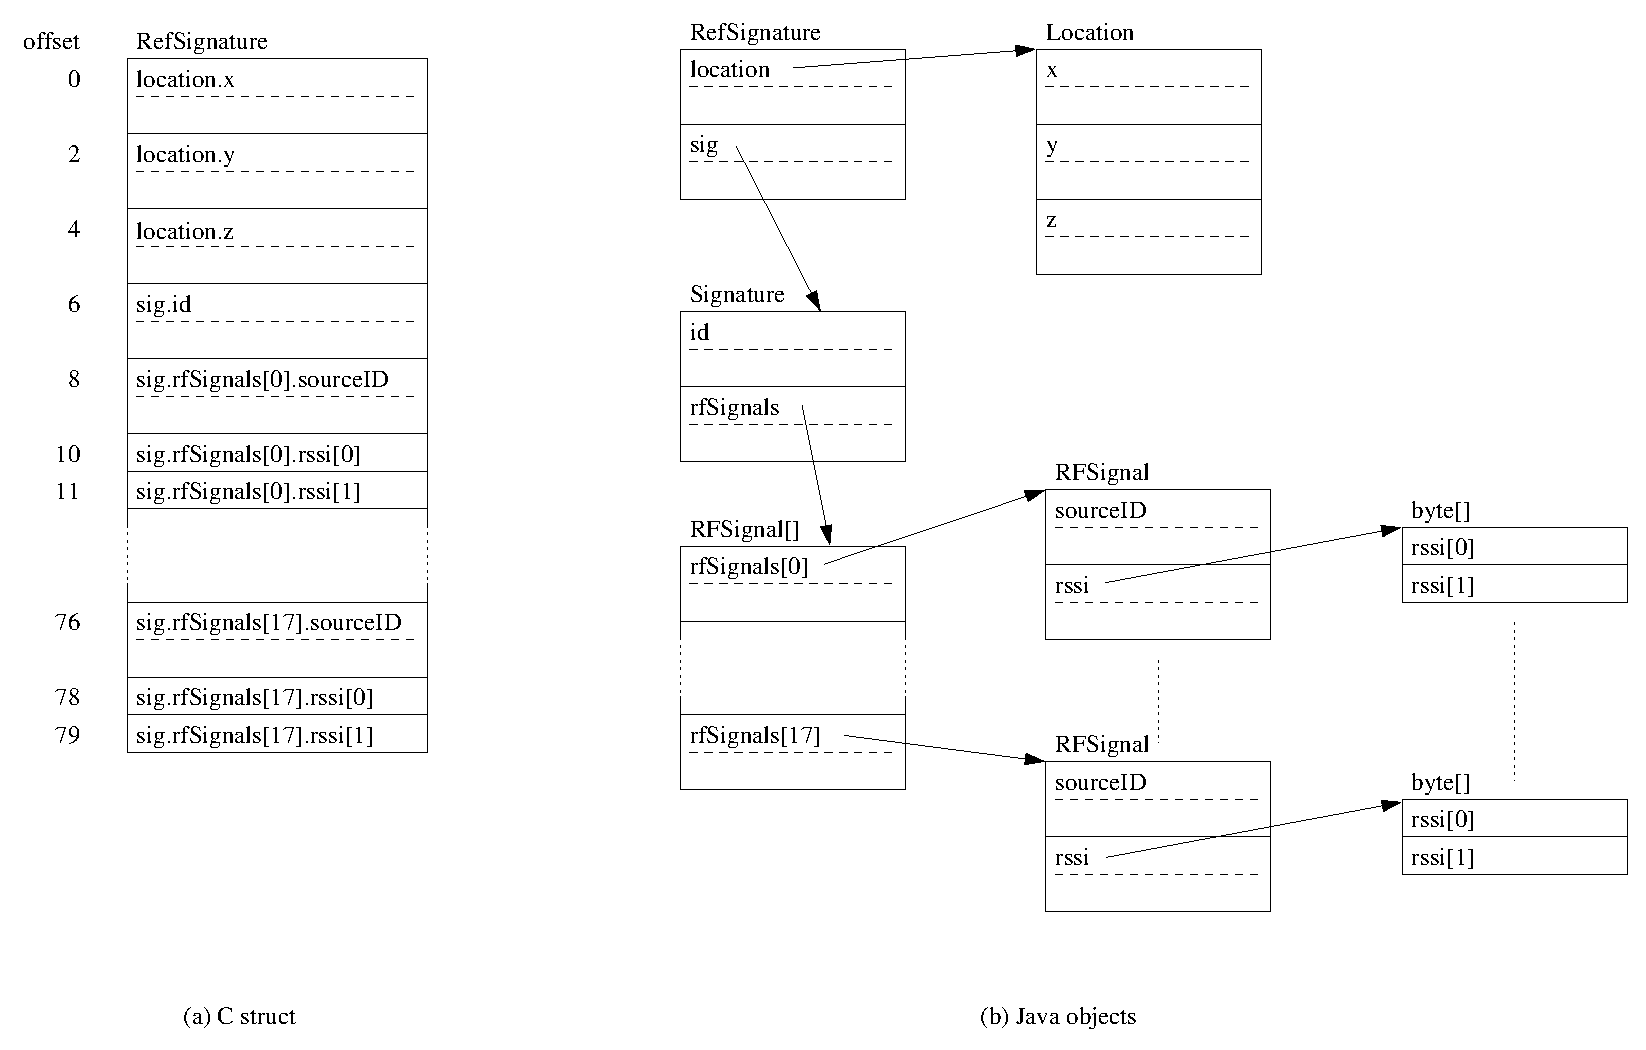
\includegraphics[width=0.9\linewidth]{motetrack-refsignature-objects}
\caption[The \mycode{RefSignature} data structure]{The \mycode{RefSignature} data structure: as a C struct, and as a collection of Java objects}
\label{fig-motetrack-refsignature-objects}
\end{figure}

Since all the arrays are of fixed length, in C the layout of the whole structure is known at compile time, shown in Figure \ref{fig-motetrack-refsignature-objects}. As described in Section \ref{sec-background-jvm-memory}, in Java every object is made up of a list of primitive values: either an int or a reference to another object. In Java we cannot have an array of objects, only an array of \emph{references to} objects. Thus, the most natural way to translate the C structures in Listing \ref{lst-motetrack-data-structure} to Java, is as a collection of objects and arrays on the heap, as shown in the right half of Figure \ref{fig-motetrack-refsignature-objects}. Note that every one of the 18 \mycode{RFSignal} structs becomes an object, which in turn has a pointer to an array of RSSI values.

There are two problems with this. First, since the location of these Java objects is not known until run time, there is a performance penalty for having to follow the chain of references. \mybench{MoteTrack} will loop over the signals in the \mycode{rfSignals} array. Starting from this array, Java needs to do 3 lookups to get to the right RSSI value: the address of the current \mycode{RFSignal} object, the address of the \mycode{rssi} array, and then the actual RSSI value. For the C version, all the offsets are known at compile time, so the compiler can generate a much more efficient loop, directly reading from the right locations.

The second problem is the added memory usage. The C struct only takes up 80 bytes, all used to store data. The Java version allocates a total of 40 objects, 36 of which are spent on the \mycode{RFSignal} objects and their arrays of RSSI values. Each of these requires a heap header, which takes up 5 bytes. In addition, the 18 byte arrays have a 3 byte header, the signal array a 4 byte header, and the whole structure contains a total of 39 references which each take up 2 bytes. In total, the collection of Java objects use $80 + 40*5 + 18*3 + 4 + 39*2 = 416$ bytes.

Combined with \mybench{MoteTrack}'s other data structures, this is too large to fit in memory, which forced us to refactor the 2 element \mycode{rssi} array into two byte variables stored directly in \mycode{RFSignal}, as explained in Section \ref{sec-evaluation-benchmark-implementation-motetrack}. This allowed us to run the benchmark, but a RefSignature still takes up 236 bytes, and reading an RSSI value still takes two lookups instead of one.

Table \ref{tbl-quantitative-results} shows the size of the main data structures used by each benchmark. For most benchmarks that operate on a handful of objects and arrays, the overhead is limited to at most tens of bytes. Besides \emph{MoteTrack}, the \emph{CoreMark} benchmark also has a significant overhead. Here the cause is the linked list of \mycode{ListHead} and \mycode{ListData} objects, each of which has a 5 byte header.

Generally, large arrays of primitive types do not suffer from this problem and can be stored with low relative overhead, but for programmes containing large numbers of small objects the overhead is significant. In some cases this can be mitigated by flattening the structure. Section \ref{sec-evaluation-coremark} described an alternative for \mybench{CoreMark} to replace the linked list with a single array, and in \mybench{MoteTrack}'s case the array of \mycode{RFSignal} objects could be replaced with three separate arrays for \mycode{sourceID}, \mycode{rssi_0} and \mycode{rssi_1}. In both cases the reduced memory overhead comes at a significant cost in readability.




\section{Better language support for shorts and bytes}
\label{sec-small-datatypes}
Because RAM is scarce, 16-bit short and single byte data types are commonly used in sensor node code. The standard JVM only has 32 and 64-bit operations, and variables and stack values are stored as 32-bit, even if the actual type is shorter. On a sensor node this wastes memory, and causes a performance overhead since most nodes have 8-bit or 16-bit architectures. Therefore, many sensor node JVMs, including Darjeeling, introduce 16-bit operations and store values in 16-bit slots.

However, this is only one half of the solution. At the language level, Java defines that an expression evaluates to 32-bits, or 64-bits if at least one operand is a \mycode{long}. Attempting to store this in a 16-bit variable will result in a `lossy conversion' error at compile time, unless explicitly cast to a \mycode{short}.

As an example, if we have 3 \mycode{short} variables, a, b, and c, and want store the sum of b and c in a, a cast is needed to avoid errors from the Java compiler:

\mycode{a=(short)(b+c);}

Passing literal integer values to a method call treats them as ints, even if they are small enough to fit in a smaller type, which results in calls like: 

\mycode{f((byte)1);}

While seemingly a small annoyance, in more complex code that frequently uses of shorts and bytes, these casts can make the code much harder to read. Table \ref{tbl-quantitative-results} shows that over 25 casts per 100 lines of code appear in some benchmarks.

\paragraph{Possible solutions}
%If we want to have an efficient sensor node VM, both from a performance and memory usage perspective, better support for data types smaller than 32-bit integers is necessary.

We argue that C-style automatic narrowing conversions would make most sensor node code more readable, but to leave the option of Java's default behaviour open, this may be implemented as new data types: declaring variable \mycode{a} as \mycode{unchecked short} would implicitly narrow to short when needed, so \mycode{a=b+c;} would not need an explicit cast, while it would if \mycode{a} is declared as a normal \mycode{short}.




\section{Simple type definitions}
\label{sec-typedef}
When developing code for a sensor node, the limited resources often result design patterns different from desktop software. In normal Java code we usually rely on objects for type safety and keeping code readable and easy to maintain. On sensor nodes, objects are expensive and we frequently make use of shorts and ints for a multitude of different tasks for which we would traditionally use objects.

In these situations we often found that our code would be much easier to maintain if there was a way to name new integer types to explicitly indicate their meaning, instead of using many of \mycode{int} or \mycode{short} variables. Having type checking on these types would add a welcome layer of safety.

\paragraph{Possible solutions}
At a minimum, there should be a way to define simple aliases for primitive types, similar to C's \mycode{typedef}. A more advanced option that fits more naturally with Java, would be to have a strict \mycode{typedef} which also does type checking, so that a value of one user defined integer type cannot be accidentally assigned to a variable of another type, without an explicit cast.




\section{Explicit and efficient inlining}
\label{sec-inlining}
Java method calls are inherently more expensive than C functions. On the desktop, JIT compilers can remove much of this overhead, but a sensor node does not have the resources for this. We often found this to be a problem for small helper functions that are frequently called. As an example, the C version of the \mybench{XXTEA} benchmark contains this macro: 

\begin{minted}{c}
    #define MX (((z>>5^y<<2) + (y>>3^z<<4)) \\
                 ^ ((sum^y) + (key[(p&3)^e] ^ z)))
\end{minted}

This macro is called in four places, and implementing it as a lightweight method still slows down the benchmark by 57\%. Tools like ProGuard \cite{proguard} can be used to inline small methods or methods that are only called from a single location, but \mycode{MX} is called from multiple places and is larger than ProGuard's size threshold. This leaves developers with two unattractive options: either leaving it as a method and accepting the performance penalty, or manually copy-pasting the code, which is error-prone and leads to code that is harder to maintain.

Inlining larger methods called from multiple locations does run the risk of increasing code size. However, the data in Table \ref{tbl-quantitative-results} shows the increase in code size is often modest. In two cases the inlined version is actually smaller. The code generated by the AOT compiler for a lightweight method call is still larger than for most other bytecode instructions, and in \emph{CoreMark}'s case inlining the \mycode{ee_isdigit} method means the code directly branches on the result of the inlined expression, instead of having to perform an additional branch on the returned boolean value.

\paragraph{Possible solutions}
Developers should be given more control over inlining, which could be achieved by an \mycode{inline} keyword to force the compiler to inline important methods.



\section{An optimising compiler}
\label{sec-optimising-javac}
As discussed in previous chapters, but listed here again for completeness, Java compilers typically do not optimise the bytecode but translate the source almost as-is. Without a clear performance model it is not always clear which option is faster, and the bytecode is expected to be run by a JIT compiler, which can make better optimisation decisions knowing the target platform and run-time behaviour. However, a sensor node does not have the resources for this and must execute the code as it is received. This leads to significant overhead, for example by repeatedly re-evaluating a constant expression in a loop.

\paragraph{Possible solutions}
Even without a clear performance model, some basic optimisations can be done. Table \ref{tbl-quantitative-results} shows the resulting performance without the manual optimisations discussed in Section \ref{sec-optimisations-manual-java-source-optimisation}. These optimisations could be further expanded, and combining the tasks of the optimiser and infuser can further improve performance as shown in Section \ref{sec-evaluation-other-platforms-word-size}.




\section{Allocating objects on stack}
\label{sec-no-gc}
In Java anything larger than a primitive value has to be allocated on the heap. This introduces a performance overhead, both for allocating the objects, and the occasional run of the garbage collector that may take several thousand cycles.

In our benchmarks we encountered a number of situations where a temporary object was needed. For example, the \mycode{encode} function in the \mybench{LEC} benchmark needs to return two values: \emph{bsi} and the number of bits in \emph{bsi}. In C this is done by passing two pointers to \mycode{encode}. In Java we can wrap both values in a class and either create and return an object from \mycode{encode}, or let the caller create it and pass it as a parameter for \mycode{encode} to fill in.

In code that frequently needs short-lived objects the overhead for allocating them can be significant, and unpredictable garbage collector runs are a problem for code with specific timing constraints. Besides \mybench{LEC}, we saw similar situations in the \mybench{CoreMark} and \mybench{MoteTrack} benchmarks. The problem is especially serious on a sensor node, where the limited amount of memory means the garbage collector is triggered frequently even if relatively few temporary objects are created.

\begin{listing}
\begin{minted}{java}
    public static short LEC(short[] numbers, Stream stream) {
        BSI bsi = new BSI();      // Allocate bsi only once
        for (...) {
            ...
            compress(ri, ri_1, stream, bsi);
            ...
        }
    }

    private static void compress(short ri, short ri_1, Stream stream, BSI bsi) {
        ...
        encode(di, bsi);          // Pass bsi to encode to return both value and length
        ...
    }

    private static void encode(short di, BSI bsi) {
        ...
        bsi.value = ...           // return value and length by setting object fields
        bsi.length = ...
    }
\end{minted}
\caption{Avoiding multiple object allocations in the LEC benchmark}
\label{lst-lec-avoiding-object-allocations}
\end{listing}

This overhead can often be reduced by allocating objects earlier and reusing the same objects in a loop. In Listing \ref{lst-lec-avoiding-object-allocations} this is implemented for the \mybench{LEC} benchmark, where the \mycode{bsi} object is used to return two values from \mycode{encode} to \mycode{compress}. Instead of creating a new object in each iteration in the \mycode{compress} method where it is needed, \mycode{bsi} is created once, outside of the main loop, and passed to \mycode{compress} multiple times.

This technique of pulling object creation up the call chain can often be used to remove this sort of overhead, and it worked in all three benchmarks mentioned before. However, it gets very cumbersome if the number of objects is more than one or two, or if they need to be passed through multiple layers. Readability is also reduced, since objects that are only needed in a specific location are now visible from a much larger scope. Table \ref{tbl-quantitative-results} shows the performance without this optimisation.

\paragraph{Possible solutions}
On desktop JVMs, escape analysis \cite{Choi:1999uw, Goetz:2005uy} is used to determine if an object can be safely allocated on the stack instead of the heap, thus saving both the cost of heap allocation, and the occasional garbage collection run triggered by it.

While the analysis of the bytecode required for this is far too complex for a sensor node, it could be done offline, similar to TakaTuka's offline garbage collector analysis \cite{Aslam:2011thesis}. The bytecode can then be extended by adding special versions of the \mycode{new} opcodes to instruct the VM to place an object in the stack frame instead of on the heap. A field should also be added to the method header to tell the VM how much extra space for stack objects needs to be reserved in the stack frame.

There is a risk to doing this automatically. In CapeVM, the split between heap and stack memory is fixed, and both are limited. If the compiler automatically puts all objects that could be on the stack in the stack frame instead of on the heap, we may end up with an empty heap, and a stack overflow. Therefore, it is better to leave this optimisation to the developer by also introducing a new keyword at the language level, so developers can explicitly indicate which objects go on the stack and which on the heap. Of course escape analysis is still necessary to check at compile time that this keyword is only used in places where it is legal for the object to be allocated on the stack.




\section{Reconsidering advanced language features}
\label{sec-advanced-features}
Finally, we conclude with some discussion on more fundamental language design choices. Many sensor node JVMs implement some of Java's more advanced features, but we are not convinced this is always a good choice on a sensor node.

While features like threads, exceptions and garbage collection are all useful, they come at a cost. The trade-off for a sensor node VM is significantly different from a desktop VM: many of Java's more advanced features are vital to large-scale software development, but the size of sensor nodes programmes is much smaller. And while VM size is not an issue on the desktop, these features are relatively expensive to implement on a sensor node with limited flash memory. We believe a VM developed from scratch, with the aim of providing platform independence, safety, and performance through AOT compilation, would end up with a design very different from the JVM.

Table \ref{tab-vm-size} shows the code size in Darjeeling for some features discussed below. This was determined by only counting the size of functions directly related to specific features. The actual cost is higher since some, especially garbage collection, also add complexity to other functions throughout the VM. Combined, the features below and the string functions mentioned in Section \ref{sec-std-lib} make up about half of the original Darjeeling VM.

Besides an increase in VM size, these features also cause a performance penalty, and features such as threads and exceptions are much harder to implement in an AOT compiler where we cannot implement them in the interpreter loop. This means that if we care about performance and the corresponding reduction in CPU energy consumption, we either have to give them up, or spend considerably more in terms of VM complexity and size.


\subsection{Threads}
As shown in Table \ref{tab-vm-size}, support for threads accounts for about 10\% of the VM size, if we exclude the string library. In addition, each thread requires a stack. If the VM allocates a fixed block, it must be large enough to avoid stack overflows, but too large a block wastes precious RAM. Darjeeling allocates each stack as a linked list of frames on the heap. This is memory efficient, but allocating on the heap is slower and will occasionally trigger the garbage collector.

A more cooperative concurrency model, where lightweight tasks voluntarily yield the CPU and share a single stack, is more appropriate for sensor nodes. This is also the approach to concurrency chosen by a number of native code systems, including \emph{t-kernel} \cite{Gu:2005un}, nesC \cite{Gay:2003up}, and more recently Amulet \cite{Hester:2016je}.


\subsection{Exceptions}
In terms of code size, exceptions are not very expensive to implement in an interpreter, but they are hard to implement in an AOT compiler. We also feel the advantage of having exceptions is much lower than the other features mentioned in this section, since they could be easily replaced with return values to signal errors.


\subsection{Virtual methods}
It is hard to quantify the overhead of implementing virtual methods since the code for handling them is integrated into several functions. In terms of size it is likely less than 2 KB, but the performance overhead is considerable. The target of a virtual method call must be resolved at run time, they cannot be made lightweight, and an AOT compiler can generate much more efficient code for calls to static methods.

In practice we seldom use virtual methods in sensor node code, but some form of indirect calls is necessary for things like signal handling. It should be possible to develop a more lightweight form of function pointers that can be implemented efficiently. However, the details will require more careful study.


\subsection{Garbage collection}
Finally, garbage collection is clearly the most intrusive aspect of the JVM to change. While the first three features could be changed with minor modifications to Java, the managed heap is at its very core.

Still, there are good reasons for considering alternatives. Table \ref{tab-vm-size} shows the garbage collector functions in Darjeeling add up to about 3.5 KB, but the actual cost is much higher as many other parts of Darjeeling are influenced by the garbage collector.

Specifically, it is the reason Darjeeling splits references and integers throughout the VM. This makes it easy for the garbage collector to find live references, but leads to significant code duplication and complexity. Using AOT compilation, the split stack adds overhead to maintain this state, and requires two extra registers as a second stack pointer that cannot be used for stack caching.




\section{Building better sensor node VMs}
In this chapter we described a number of issues we encountered over the years while using and developing sensor node VMs. They may not apply to every scenario, but the wide range of the issues presented here, and the data in Table \ref{tbl-quantitative-results}, suggest many applications will be affected by at least some.

Most sensor node VMs already modify the instruction set of the original VM and usually support only a subset of the original language. The issues described here indicate these changes do not go far enough, and we still need to refine our VMs further to make them truly useful in real-world projects.

There are two possible paths to follow: a number of issues can be solved by improving existing Java-based VMs. Staying close to Java has the advantage of being able to reuse existing knowledge and infrastructure.

However some of the issues require more invasive changes to both the source language and VM. If the goal is to run platform independent code safely and efficiently, rather than running Java, we should start from the specific requirements and constraints of sensor node software development, which would lead to more lightweight features and a more predictable memory model.

For either path, we hope the points presented in this chapter can help in the development of better future sensor node VMs.

\chapter{Conclusion}
This dissertation described the CapeVM sensor node virtual machine. CapeVM extends the state of the art by combining the desirable features of platform independent reprogramming, a safe execution environment, and acceptable performance. CapeVM was evaluated using a set of benchmarks, including small benchmarks to highlight specific behaviours, and five examples of real sensor node applications.

To come back to the research questions stated in Section \ref{sec-introduction-research-questions}, we can conclude the following:

\begin{enumerate}
	\item[a.]
	After identifying the sources of overhead in previous work on ahead-of-time compilers for sensor nodes, CapeVM introduced a number of optimisations to reduce the performance overhead by over 79\%, and the code size overhead by 60\%, resulting in an average performance overhead of 70\%, and the code size overhead of 79\% compared to native C.

	The optimisations introduced by CapeVM do increase the size of the VM, but the break-even point at which this is compensated for by the smaller code it generates, is well within the range of programme memory typically available on a sensor node.

	The price to pay for platform independence and a safe execution environment comes in three forms. There is still a performance overhead, but it is at a level that will be acceptable for many applications. The increase in code size however, and the space taken by the VM, do limit the size of applications we can load onto a device. Finally, the overhead in memory usage is a problem for programmes allocating many small objects.

	\item[b.]
	CapeVM's second contribution is providing a safe execution environment. Compared to native binary code, the higher level of abstraction of CapeVM's bytecode allowed us to develop a relatively simple set of safety checks.
	
	This results in a modest overhead in terms of VM size, and because most checks are performed at translation time, the overhead for providing safety is limited to a slowdown of 22\% and a 2\% increase in code size, compared to the unsafe version.
	
	Since to the best of our knowledge only two native code approaches exist that provide safety independent of the host, we cannot exclude the possibility that these could be further optimised. Currently however, CapeVM is on-par with or faster than existing systems, and provides platform independence at the same time.

	\item[c.]
	Regarding the question of whether Java is a suitable language for a sensor node VM, we can conclude some aspects of it are a good match. An advantage of its simple stack-based instruction set is that it can be implemented in a small VM, and while we showed the stack-based architecture introduces significant overhead, most of this overhead is eliminated by our optimisations.
	
	However, our benchmarks also exposed several problems that ultimately make standard Java a poor choice. Specifically, the lack of support for constant data, and the inefficient use of memory for programmes containing many small objects meant some benchmarks could not be ported directly from C to Java. We proposed several improvements, and developed an extension to allow constant data to be put in flash memory, but conclude that more work is necessary to come to a more sensor node specific language and make sensor node VMs truly useful in a wide range of real-world projects.
\end{enumerate}

\begin{table}
\caption{Comparison of CapeVM to related work}
\label{tbl-contribution-comparison}
    \begin{threeparttable}
    \begin{tabular}{lrrrrrrrr} % UPDATED 20180327
    \toprule
    Approach          & Platform    & Safe               & Performance           & Code size                  \\
                      & indep.      &                    &                       &                            \\
    \midrule
    \midrule
    Native code       & No          & No                 & 1x                    & 1x                         \\
    Interpreters      & Yes         & Mostly no          & 300-55400\% slower    & ~50\% smaller \tnote{b}    \\ 
    % Most interpreters & Yes         & No                 & 1300-22900\% slower   & ~50\% smaller \tnote{b}    \\
    % SensorScheme      & Yes         & Yes                & 300-10400\% slower    & unknown \tnote{b}          \\
    Ellul's AOT       & Yes         & No                 & 204-1927\% slower     & 26-449\% larger \tnote{b}  \\
    Safe TinyOS       & No          & Yes \tnote{a}      & 17\% slower           & 27\% larger                \\
    Harbor            & No          & Yes                & 380 to 1230\% slower  & 30 to 65\% larger          \\
    \emph{t-kernel}   & No          & Yes                & 50 to 200\% slower    & 500 to 750\% larger        \\
    CapeVM (unsafe)   & Yes         & No                 & 67\% slower           & 77\% larger                \\ % avg
    CapeVM (safe)     & Yes         & Yes                & 105\% slower          & 82\% larger                \\ % avg
    \bottomrule
    \end{tabular}
    \begin{tablenotes}
        \item[a] requires a trusted host
        \item[b] no support for constant data
    \end{tablenotes}
    \end{threeparttable}
\end{table}


Finally, we conclude by comparing our approach to existing work on improving sensor node VM performance, and on safe execution environments in Table \ref{tbl-contribution-comparison}.

Taking unsafe and platform specific native C as a baseline, we first note that existing interpreting sensor node VM's are typically not safe, and suffer from a 1 to 2 orders of magnitude slowdown. The performance overhead was reduced drastically by Ellul's work on Ahead-of-Time compilation, but still a significant overhead remains and this approach increases code size, reducing the size of programmes we can load onto a device.

On the safety side, Safe TinyOS achieves safety with relatively little overhead, but this depends on a trusted host. Harbor and \emph{T-kernel} provide safety independent of the host, but at the cost of a significant performance overhead, or increase in code size respectively. Non of these approaches provide platform independence.

Finally, we see CapeVM provides both platform independence and safety, at a cost in terms of code size and performance that is lower than or comparable to previous work.

%TODO: discuss with prof. Shih whether to include SensorScheme in Table 9.1

%TODO: check for consistent use of WSN/IoT/wireless sensor networks/sensor networks/Internet-of-Things
%TODO: check for 'we', 'our', etc
%TODO: check for VM and replace with virtual machine?
%TODO: consistent use of AVR or ATmega.
%TODO: consistent use of (sensor) node and device

%TODO: discuss with prof Shih (1) include SensorScheme in conclusion table?


\appendix
\chapter{LEC benchmark source code}
\label{app-lec-source}
\inputminted[breaklines=true]{java}{A01-code-lec.java}
\captionof{listing}{LEC benchmark source code}

\chapter{Outlier detection benchmark source code}
\label{app-outlier-detection-source}
\inputminted[breaklines=true]{java}{B01-code-outlier.java}
\captionof{listing}{Outlier detection benchmark source code}

\chapter{Heat detection benchmark source code}
\label{app-heat-detection-source}

\section{Calibration}
\inputminted[breaklines=true]{java}{C01-code-heat-calib.java}
\captionof{listing}{Heat detection benchmark source code (calibration phase)}

\section{Detection}
\inputminted[breaklines=true]{java}{C02-code-heat-detect.java}
\captionof{listing}{Heat detection benchmark source code (detection phase)}


\backmatter

\addcontentsline{toc}{chapter}{\bibname}
\bibliographystyle{abbrv}

% Your bibliography goes here
\bibliography{references}

\end{document}
